\documentclass[UTF8]{article}
\usepackage{geometry}                % See geometry.pdf to learn the layout options. There are lots.
\geometry{a4paper}                   % ... or a4paper or a5paper or ... 

%\geometry{landscape}                % Activate for for rotated page geometry
\usepackage{graphicx}
\usepackage{graphbox}
\usepackage{hyperref}
\usepackage{amssymb}
\usepackage{epstopdf}
\usepackage{algorithm}
\usepackage[noend]{algpseudocode}
\usepackage{enumitem}
\usepackage[acronym]{glossaries}
\usepackage[hang,footnotesize,bf]{caption}
\DeclareGraphicsRule{.tif}{png}{.png}{`convert #1 `dirname #1`/`basename #1 .tif`.png}


% Copied from Stack Exchange for ToDo items
% -----------------------------------------------------------
\usepackage{xargs} 
\usepackage[pdftex,dvipsnames]{xcolor}  % Coloured text etc.
% 
\usepackage[colorinlistoftodos,prependcaption,textsize=tiny]{todonotes}
\newcommandx{\unsure}[2][1=]{\todo[linecolor=red,backgroundcolor=red!25,bordercolor=red,#1]{#2}}
\newcommandx{\change}[2][1=]{\todo[linecolor=blue,backgroundcolor=blue!25,bordercolor=blue,#1]{#2}}
\newcommandx{\info}[2][1=]{\todo[linecolor=OliveGreen,backgroundcolor=OliveGreen!25,bordercolor=OliveGreen,#1]{#2}}
\newcommandx{\improvement}[2][1=]{\todo[linecolor=Plum,backgroundcolor=Plum!25,bordercolor=Plum,#1]{#2}}
\newcommandx{\thiswillnotshow}[2][1=]{\todo[disable,#1]{#2}}


\title{Validator Economics: Variable min validator deposit size\\
\vspace{4pt}
\large EF Academic Grant ID: FY23-1030\\
\vspace{16pt}
DATA SOURCES \& GATHERING}
\vspace{16pt}
\author{Sandra Johnson\\
ConsenSys Software R\&D}
\date{\today}                                           % Activate to display a given date or no date

\begin{document}
\maketitle


% Acronym definitions
\newacronym{apr}{APR}{annual percentage rate}
\newacronym{ef}{EF}{Ethereum Foundation}
\newacronym{mev}{MEV}{maximal extractable value}
\newacronym{rig}{RIG}{Rigorous Incentives Group}
\newacronym{ssf}{SSF}{single slot finality}

% ------------------------------------------------------------------------------
\section{Overview}
% ------------------------------------------------------------------------------
This document is joint work with Kerrie Mengersen and Patrick O'Callaghan, and details available information, data sources, and proposed visualisations that will provide relevant data insights to gain a deeper understanding of current validator economics and any intuitions or assumptions used in formulating proposed solutions to capping the number of validators. 

The information gathering is targeted towards the proposal being evaluated, viz. a variable minimum validator balance, which is one of the proposals that Vitalik articulated in his blog post regarding \gls{ssf} 

As the project progresses and additional data requirements are identified, this document will be updated accordingly.

Many people have generously contributed time and data, and made helpful suggestions, which has been incredibly helpful in compiling the resources listed in this document. They include, but are not limited to Barnabé Monnot and the \gls{rig} team, Justin Drake, Alexander Tesfamichael, Ben Edgington, Paul Harris and Josh Fernandez.

\section{Data Sources}
% ==================
\label{sec:sources}
% ---------------------------------------------------------------
\subsection{Key data points}
% --------------------------------------------------------------
\begin{itemize}
\item The beacon chain \textbf{deposit contract address} is: 0x00000000219ab540356cBB839Cbe05303d7705Fa 
\item The beacon chain \textbf{genesis block number} is 11182202
\end{itemize}

% ----------------------------------------------------------
\subsection{Client and staking pool diversity}
% ---------------------------------------------------------
\label{sec:diversity}
\begin{itemize}
	\item \textit{\href{https://clientdiversity.org/}{Diversify Now}} dashboard by \textit{\href{https://etheralpha.org/}{Ether alpha}} displays the current client distribution in the Consensus and Execution layers. (Figure~\ref{fig:CLELdiversity}, page~\pageref{fig:CLELdiversity}).
	\item \textit{\href{https://migalabs.es/beaconnodes}{Beacon Chain Network Public Dashboard}} by \textit{\href{https://migalabs.es/}{Miga Labs}} has several visualisations: 
	\begin{itemize}
		\item Client diversity  (Figure~\ref{fig:diversity}(a), page~\pageref{fig:diversity})
		\item Client diversity evolution (Beacon chain client distribution over time) (Figure~\ref{fig:diversity}(b), page~\pageref{fig:diversity})
		\item OS distribution of active nodes (Figure~\ref{fig:active}(a), page~\pageref{fig:active})
		\item Geographical representation of client evolution over time  (Figure~\ref{fig:active}(b), page~\pageref{fig:active})
		\item Active nodes round trip time distribution (RTT) (Figure~\ref{fig:rtt}(a), page~\pageref{fig:rtt})
		\item Graphical distribution (Beacon chain node distribution)  (Figure~\ref{fig:rtt}(b), page~\pageref{fig:rtt})
		\item RTT distribution (Figure~\ref{fig:aass}(a), page~\pageref{fig:aass})
		\item Advertised attestation subnets subscription (Figure~\ref{fig:aass}(b), page~\pageref{fig:aass})
		\item Number of beach nodes per IP (Figure~\ref{fig:ipdist}), page~\pageref{fig:ipdist})
	\end{itemize}
However, it is important to note that it is challenging to measure peer types in the network, and therefore the figures are at best approximations based on the information at hand. 

\end{itemize}	
% ---------------------------------------------------------
 \subsection{Total ETH Supply}
 % ---------------------------------------------------------
\label{sec:ethsupply} 
        The total supply of ETH used to be fairly simple to work out, but it is now more complicated for two main reasons:  implementation of EIP-1559 and the Merge.
Currently we are ``(a) burning ETH via the base fee and (b) the issuance is variable depending on the number of validators.'' (Ben Edgington 2023). 
\begin{itemize}
	\item Ultrasound is considered a credible source for total ETH supply projections. \\\textit{\href{https://ultrasound.money/}{Ultra sound money}} visualises various aspects of Ether supply since the Merge, gas, supply projections, the burn, total value secured - TVS and monetary premium. See figures~\ref{fig:ethsupply}~-~\ref{fig:monetary}, on pages~\pageref{fig:ethsupply}~-~\pageref{fig:monetary}.  

\begin{itemize}
	\item Ultrasound supplied two datasets for our analysis - the first had total supply at a more accurate and finer grained level, but shorter time period and the second dataset had data points roughly every 1,000 epochs covering from soon after Beacon chain genesis. The latter dataset is from Glassnode and would not be as accurate as the initial data provided by Alex Tesfamichael from Ultrasound.
\end{itemize}
	\item \textit{\href{https://etherscan.io/chart/ethersupplygrowth}{Etherscan}} is a good source of historic data for the growth in Ether supply since 2015. There are several pages of detailed information and the \textit{Charts \& Statistics} webpage has several visualisations, often with the ability to select different time ranges and a link to download the raw data as csv files, providing that Etherscan is acknowledged when these datasets are used.\\
	Figures~\ref{fig:ethscan}~to~\ref{fig:ethgrowth} on pages~\pageref{fig:ethscan}~to~\pageref{fig:ethgrowth} show the visualisations that are currently available.
\end{itemize}
% ---------------------------------------------------------	
\subsection{Multiple datasets}
% ---------------------------------------------------------
There are several resources that contain lists and visualisations of a variety of data from Ethereum Mainnet. Obtaining the raw data used on the websites and dashboards are not always easily accessible.
\label{sec:multiple}
\begin{itemize}
	\item \textit{\href{https://beaconcha.in/}{beaconcha.in}}, an open source Ethereum explorer, is a rich and informative resource providing visualisations and summary statistics of various aspects of the chain. It is not clear if it is possible to gain access to the data used to generate the many graphs and summary statistics. The website currently contains the following:
	\begin{itemize}
		\item On the home page, there is a \textbf{progress line} at the top of the page showing the \textit{number of slots left in the current epoch}. (Figure~\ref{fig:bhomepg}, page~\pageref{fig:bhomepg})
		\item Immediately below the progress line, there is a \textbf{summary line} showing the \textit{current epoch number}, the \textit{last finalised epoch}, the \textit{current slot number}, the \textit{number of active and pending validators}, the \textit{total staked ETH} and the \textit{average validator balance}. (Figure~\ref{fig:bhomepg})
		\item Below this summary there is a \textbf{graph} of the \textit{number of active validators} and \textit{staked ETH} for the last week (Figure~\ref{fig:bhomepg})
		\item Then there are two side by side tables. The \textbf{left table} has information about the most recent epochs: \textit{epoch number, time, whether it is final, the eligible ETH, the number of percentage of votes}. The \textbf{right table} has information about the most recent blocks: \textit{epoch number, slot number, blockfigu number, status of the block (proposed or missed), time} and the \textit{proposer id}. These two tables are shown in Figure~\ref{fig:bhomepg2}, page~\pageref{fig:bhomepg2}).\\
		\item Moreover, one can click on the epoch, slot and block numbers in the tables to obtain a detailed view of the epoch, slot or block number. 
		\item There is also a link to the validator ID in the right table that provides a detailed view of that validator.
		\item Figures~\ref{fig:bepochs}~-~\ref{fig:bmempool} on pages~\pageref{fig:bepochs}~-~\pageref{fig:bmempool} gives detailed blockchain data.
		\item Figures~\ref{fig:bvalidators}~-~\ref{fig:bblschgs} on pages~\pageref{fig:bvalidators}~-~\pageref{fig:bblschgs} gives detailed validator data.
		\item Beaconcha.in provide additional visualisations and tools. For example, the ability to generate graphs to show the correlation between two variables (Figure~\ref{fig:bcorrelations} on page~\pageref{fig:bcorrelations}.
	\end{itemize}

	\item \textit{\href{https://mevboost.pics/data.html}{Mevboost.pics - Open Data}} will eventually provide links to download several datasets: 
		\begin{itemize}
			\item \textit{eth\_data} - Slots since Merge with additional MEV-Boost and validator info such as: date, slot, block number, relay, builder pubkey, proposer pubkey, mevboost value, builder, validator \textit{(Available now)}
			\item \textit{pubkey\_mapping} - Validator public keys mapped to known entities such as Lido, Kraken ect. \textit{(Not available)}
			\item \textit{tc\_txs} - Tornado Cash related transactions \textit{(Not available)}
			\item \textit{staking\_txs} - Deposit transactions to the ETH2 Deposit contract \textit{(Not available)}
			\item \textit{relays\_over\_time} - Number of successfully relayed blocks per day \textit{(Not available)}
			\item \textit{builders\_over\_time} - Number of successfully built blocks per day \textit{(Not available)}
		\end{itemize}
\end{itemize}
% ---------------------------------------------------------
\subsection{Stakers and Staking pools}
% ---------------------------------------------------------
\label{sec:stakers}
\begin{itemize}
	\item \textbf{Data from an archive node} \\
	We had access to a teku-besu archive node, \texttt{teku-besu-ohio-mainnet-archive-01},  against which we were able to run many API queries to provide some rich data.\\
	 We ran API calls from those listed in GitHub: \href{https://ethereum.github.io/beacon-APIs/?urls.primaryName=dev}{Eth Beacon Node API}
\end{itemize}
\clearpage
% ---------------------------------------------------------------
\subsection{Existing visualisations}
% --------------------------------------------------------------
\subsubsection*{Diversify Now}
% --------------------------------------

\begin{figure}[htbp]
\begin{center}
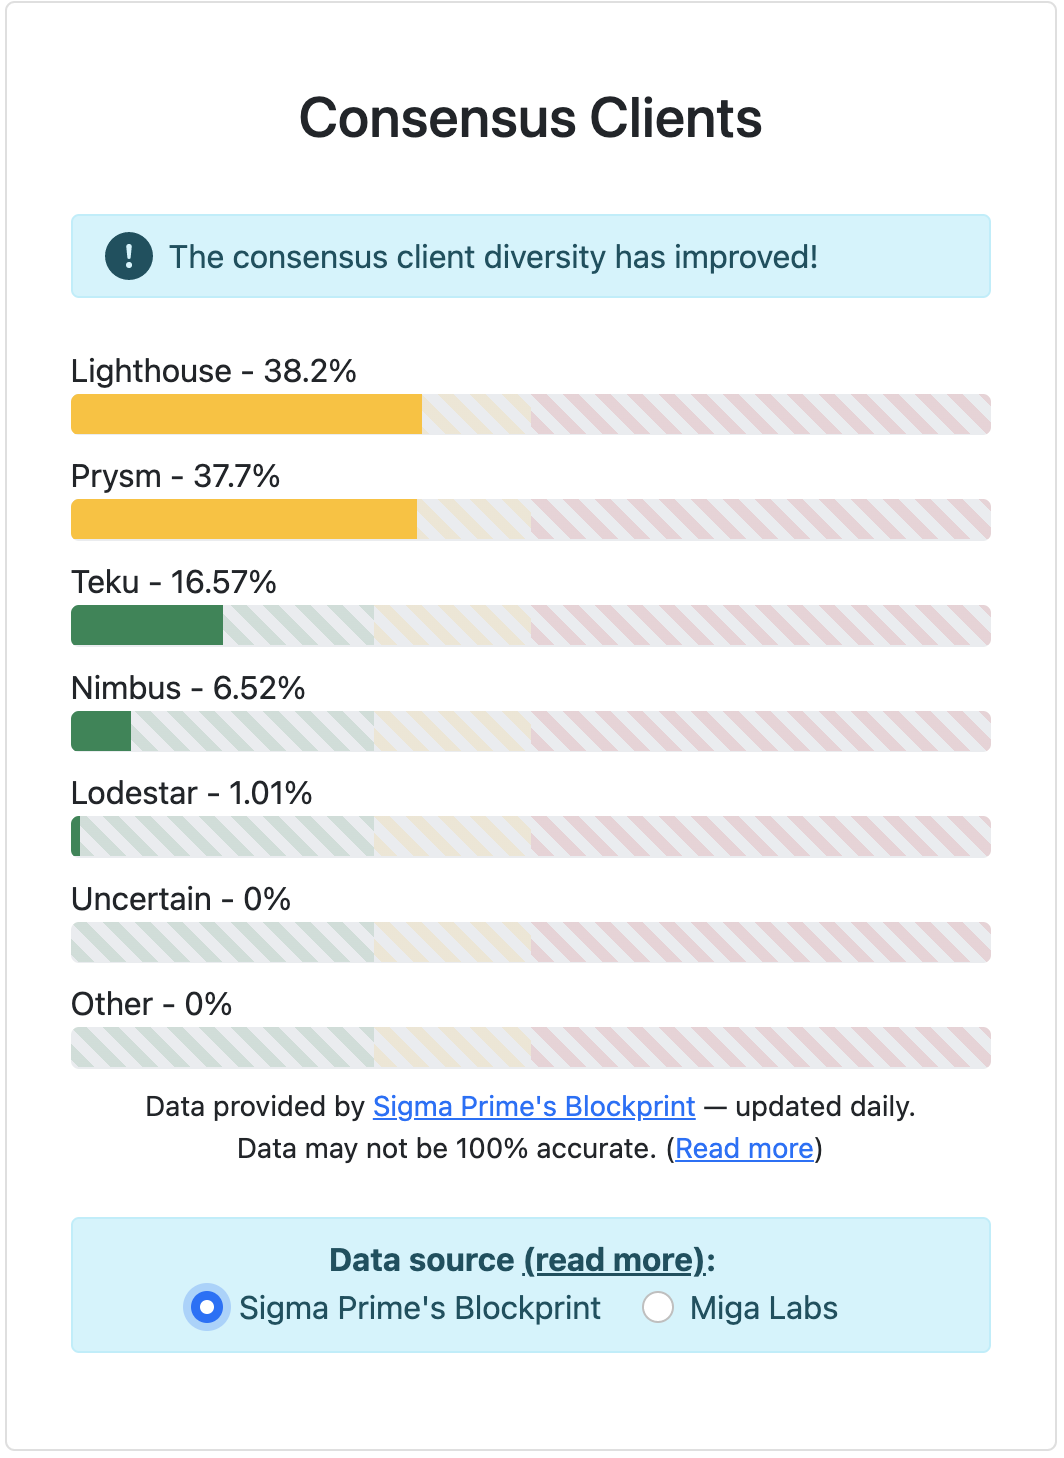
\includegraphics[width=0.3\linewidth, align=c]{images/CL-sigma}
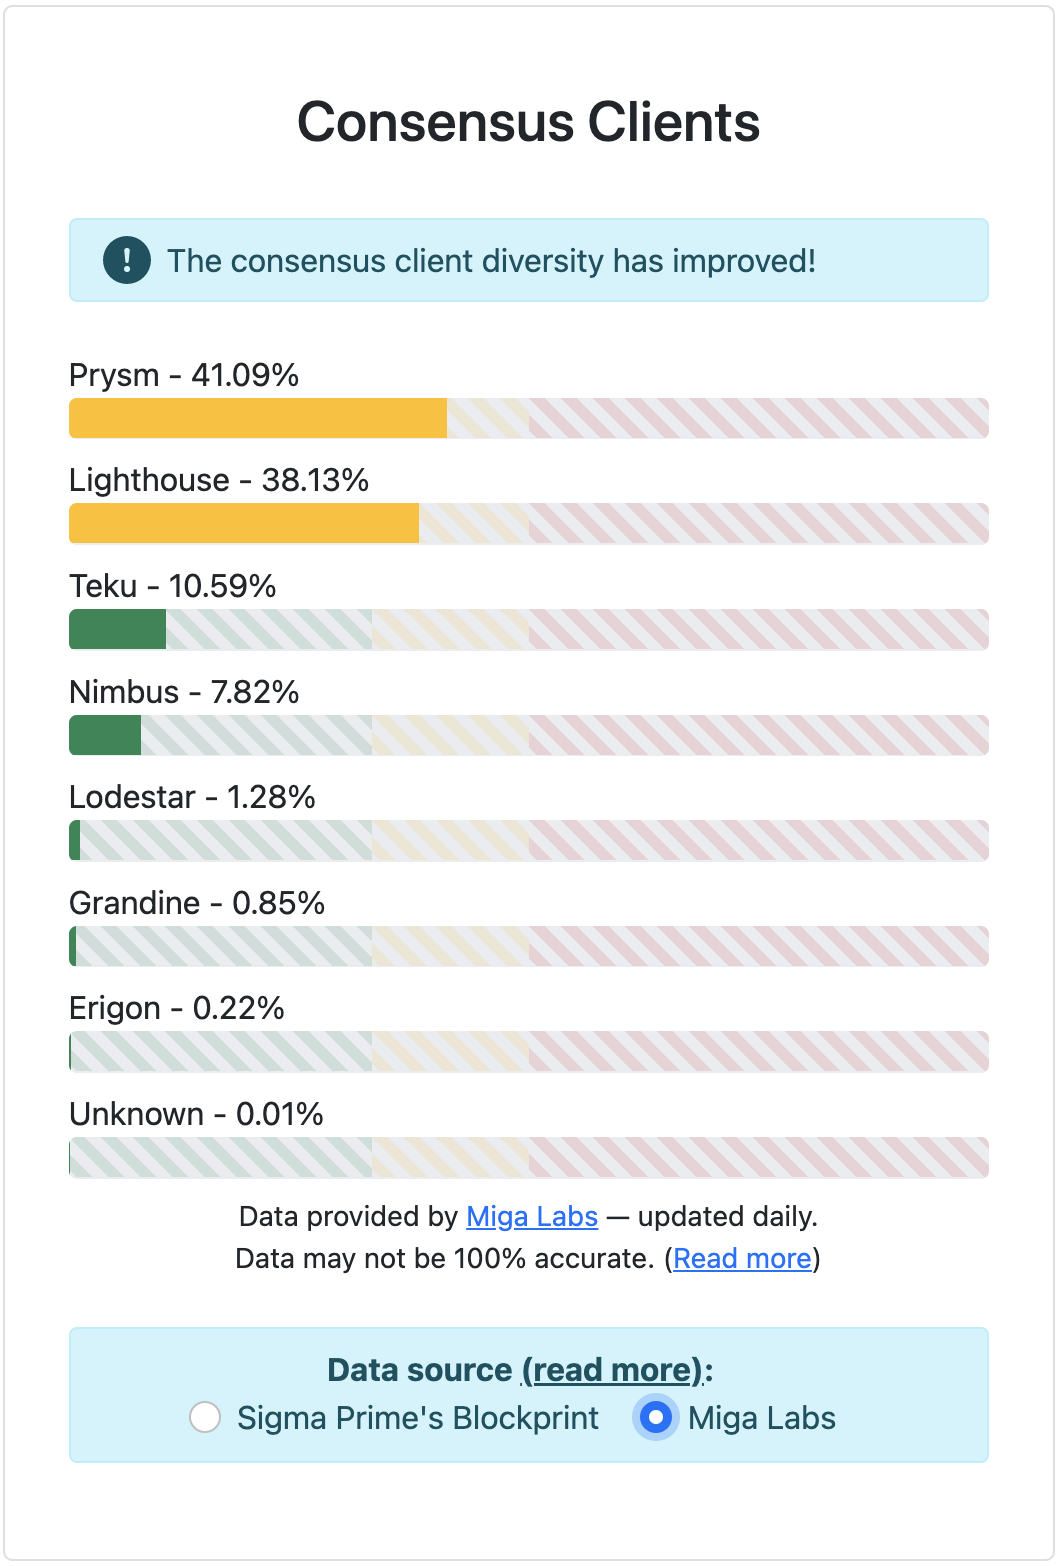
\includegraphics[width=0.3\linewidth, align=c]{images/CL-migalabs}
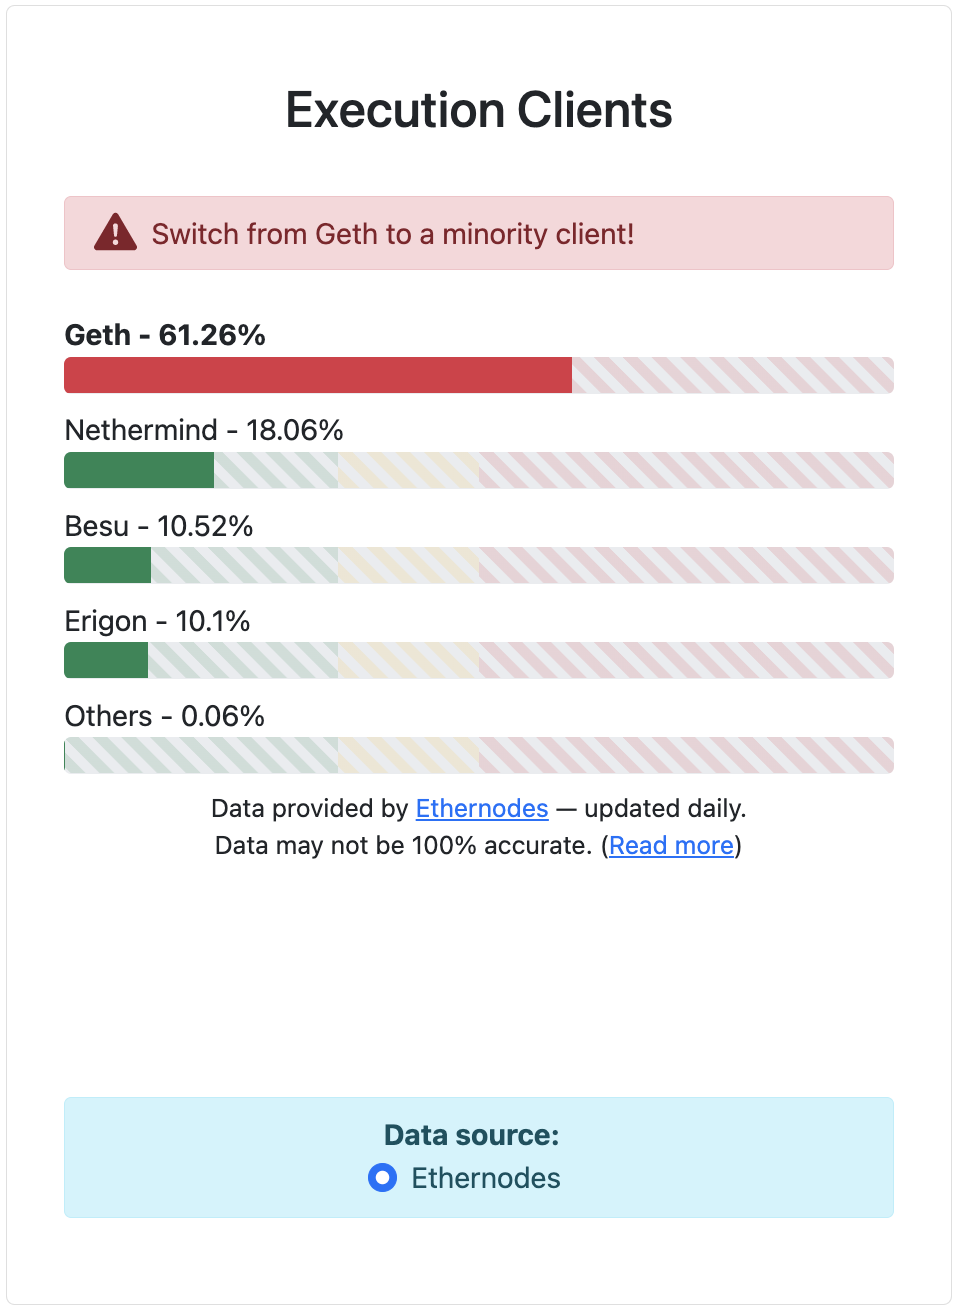
\includegraphics[width=0.3\linewidth, align=c]{images/EL-diversity}\\
(a)\hspace{110pt}        (b)\hspace{110pt} (c)\\
\caption{Consensus layer client diversity using Sigma Prime's Blockprint data (a) and using Migalabs data (b). Execution layer client diversity using Ethernodes data (19 May 2023)}
\label{fig:CLELdiversity}
\end{center}
\end{figure}
\clearpage
% --------------------------------------
\subsubsection*{Migalabs}
% --------------------------------------
 \begin{figure}[htbp]
\begin{center}
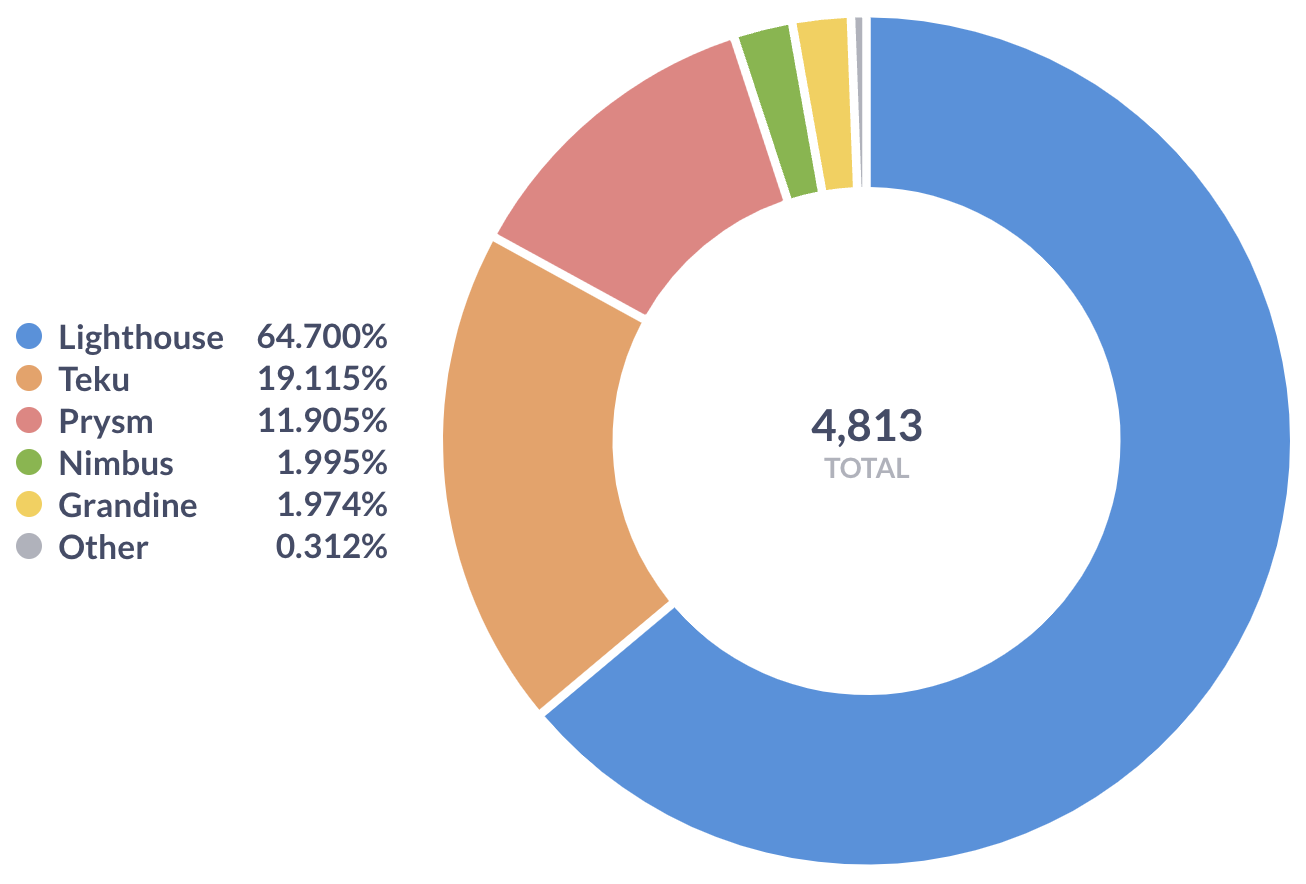
\includegraphics[width=0.48\linewidth]{images/clientdiversity}
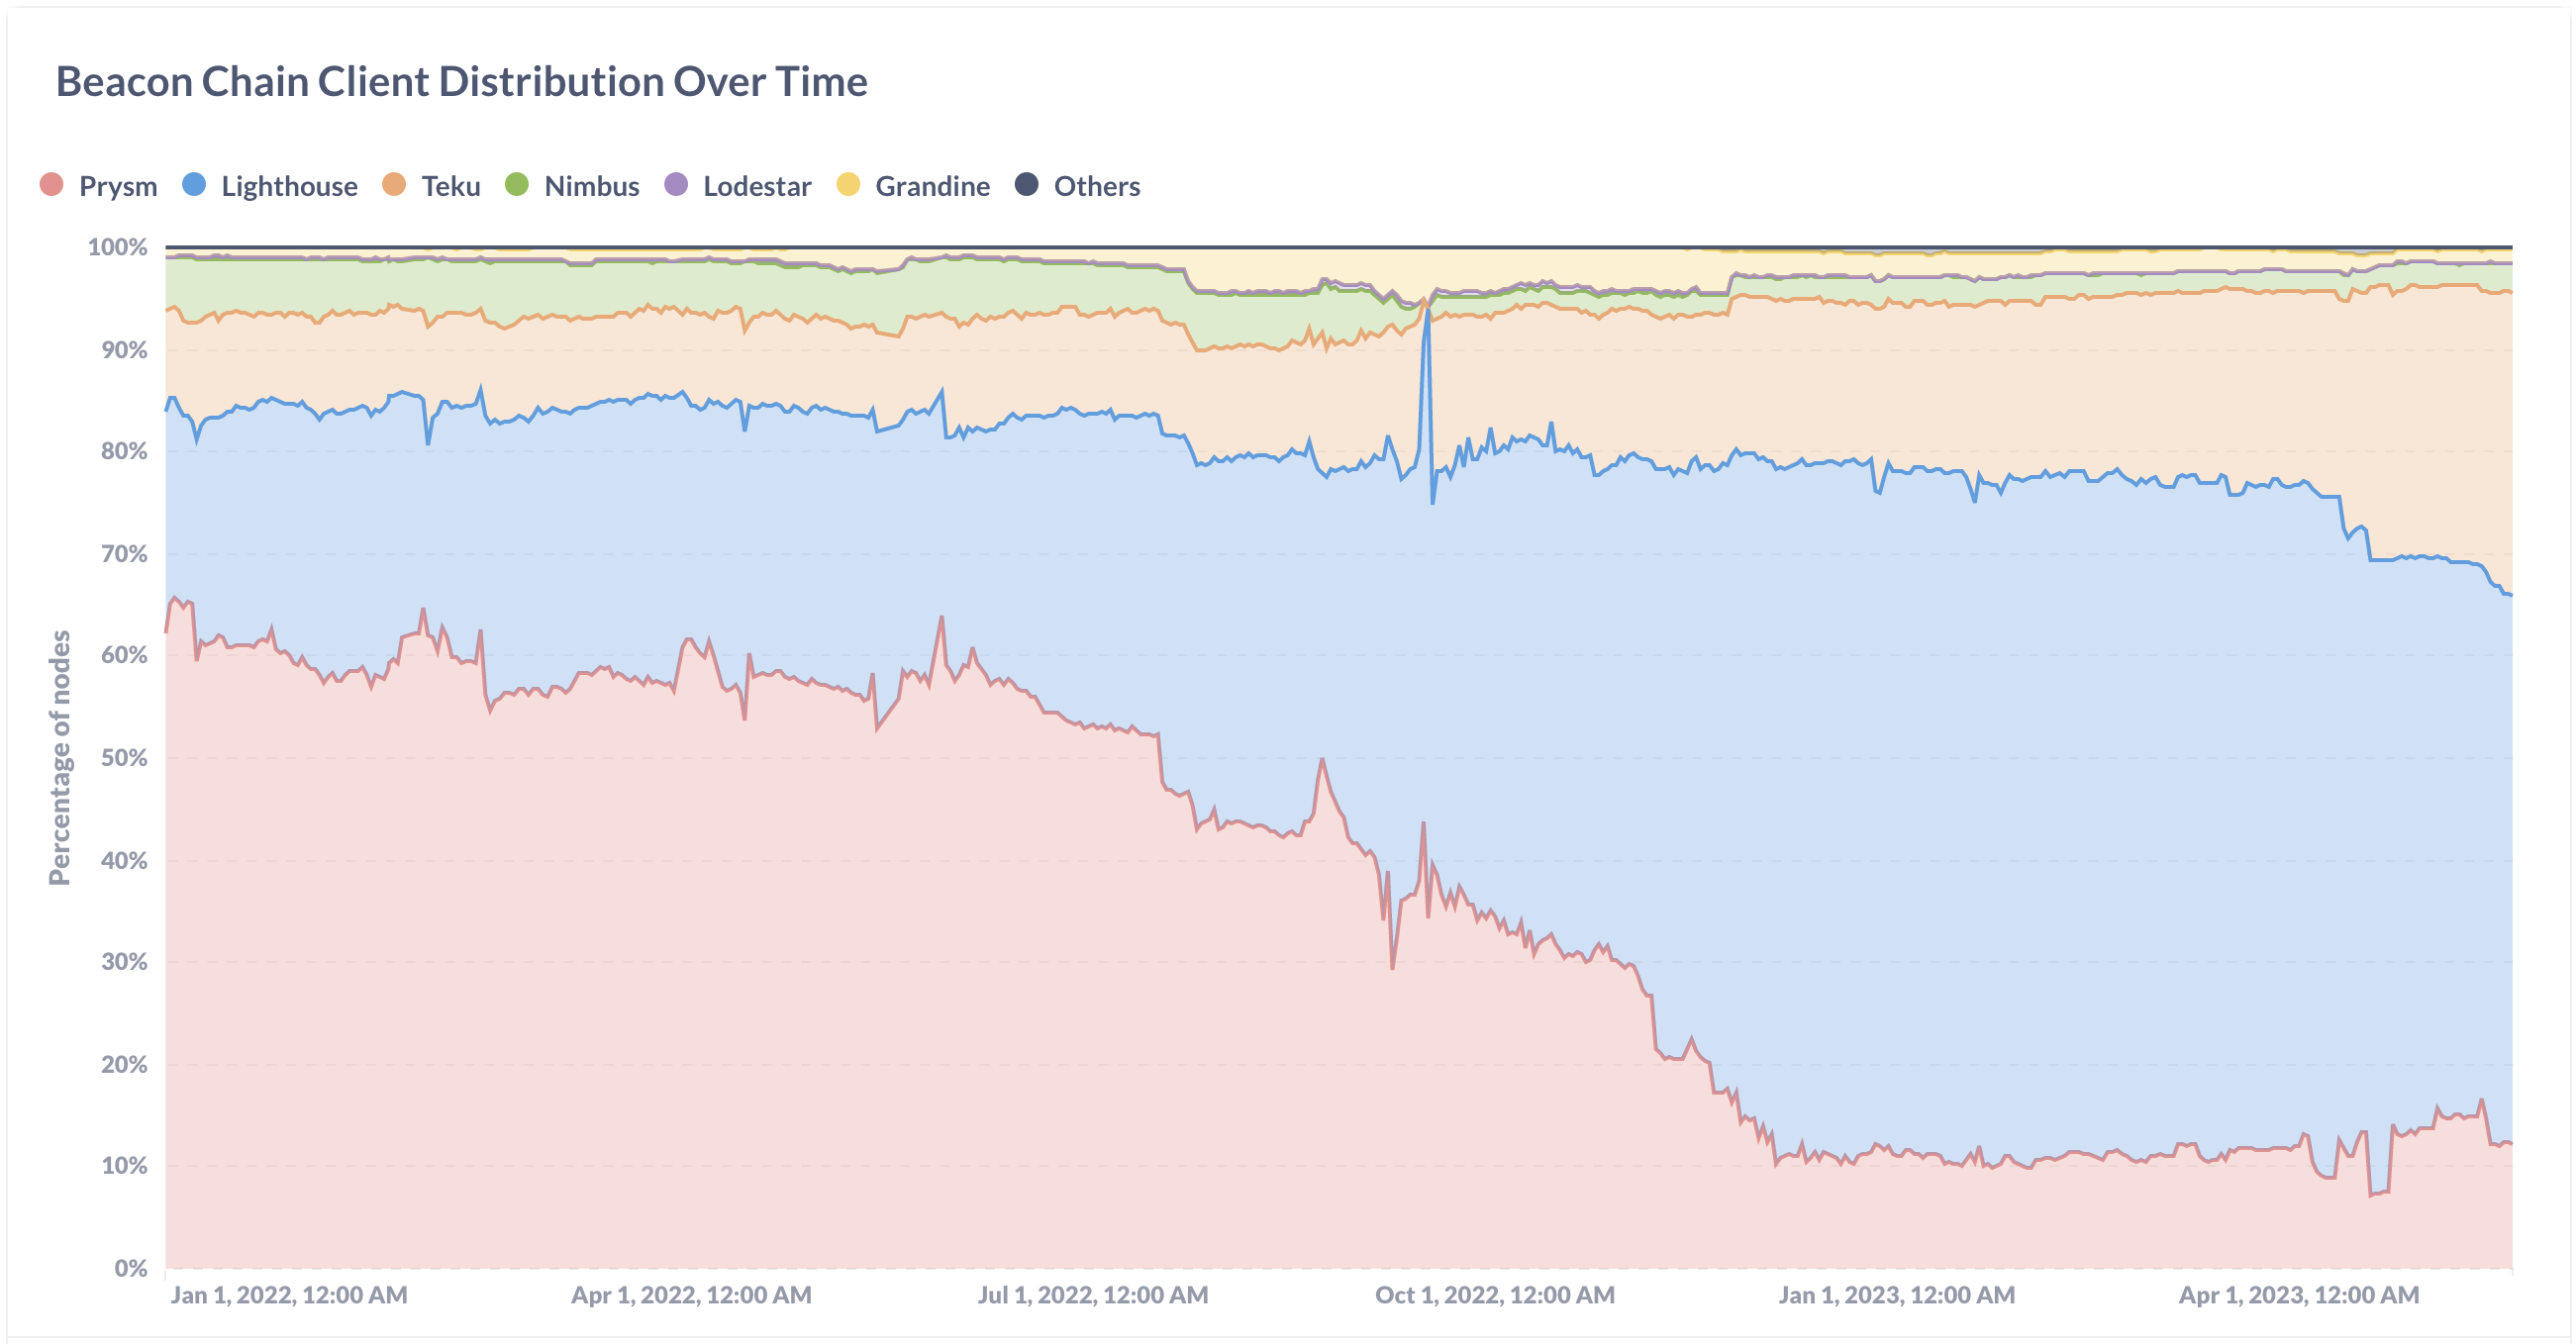
\includegraphics[width=0.48\linewidth]{images/architecture} \\
(a)\hspace{160pt}        (b)\\
\caption{Beacon chain client diversity from Migalabs (a) and client distribution over time (b) (9 May 2023)}
\label{fig:diversity}
\end{center}
\end{figure}

\begin{figure}[htbp]
\begin{center}
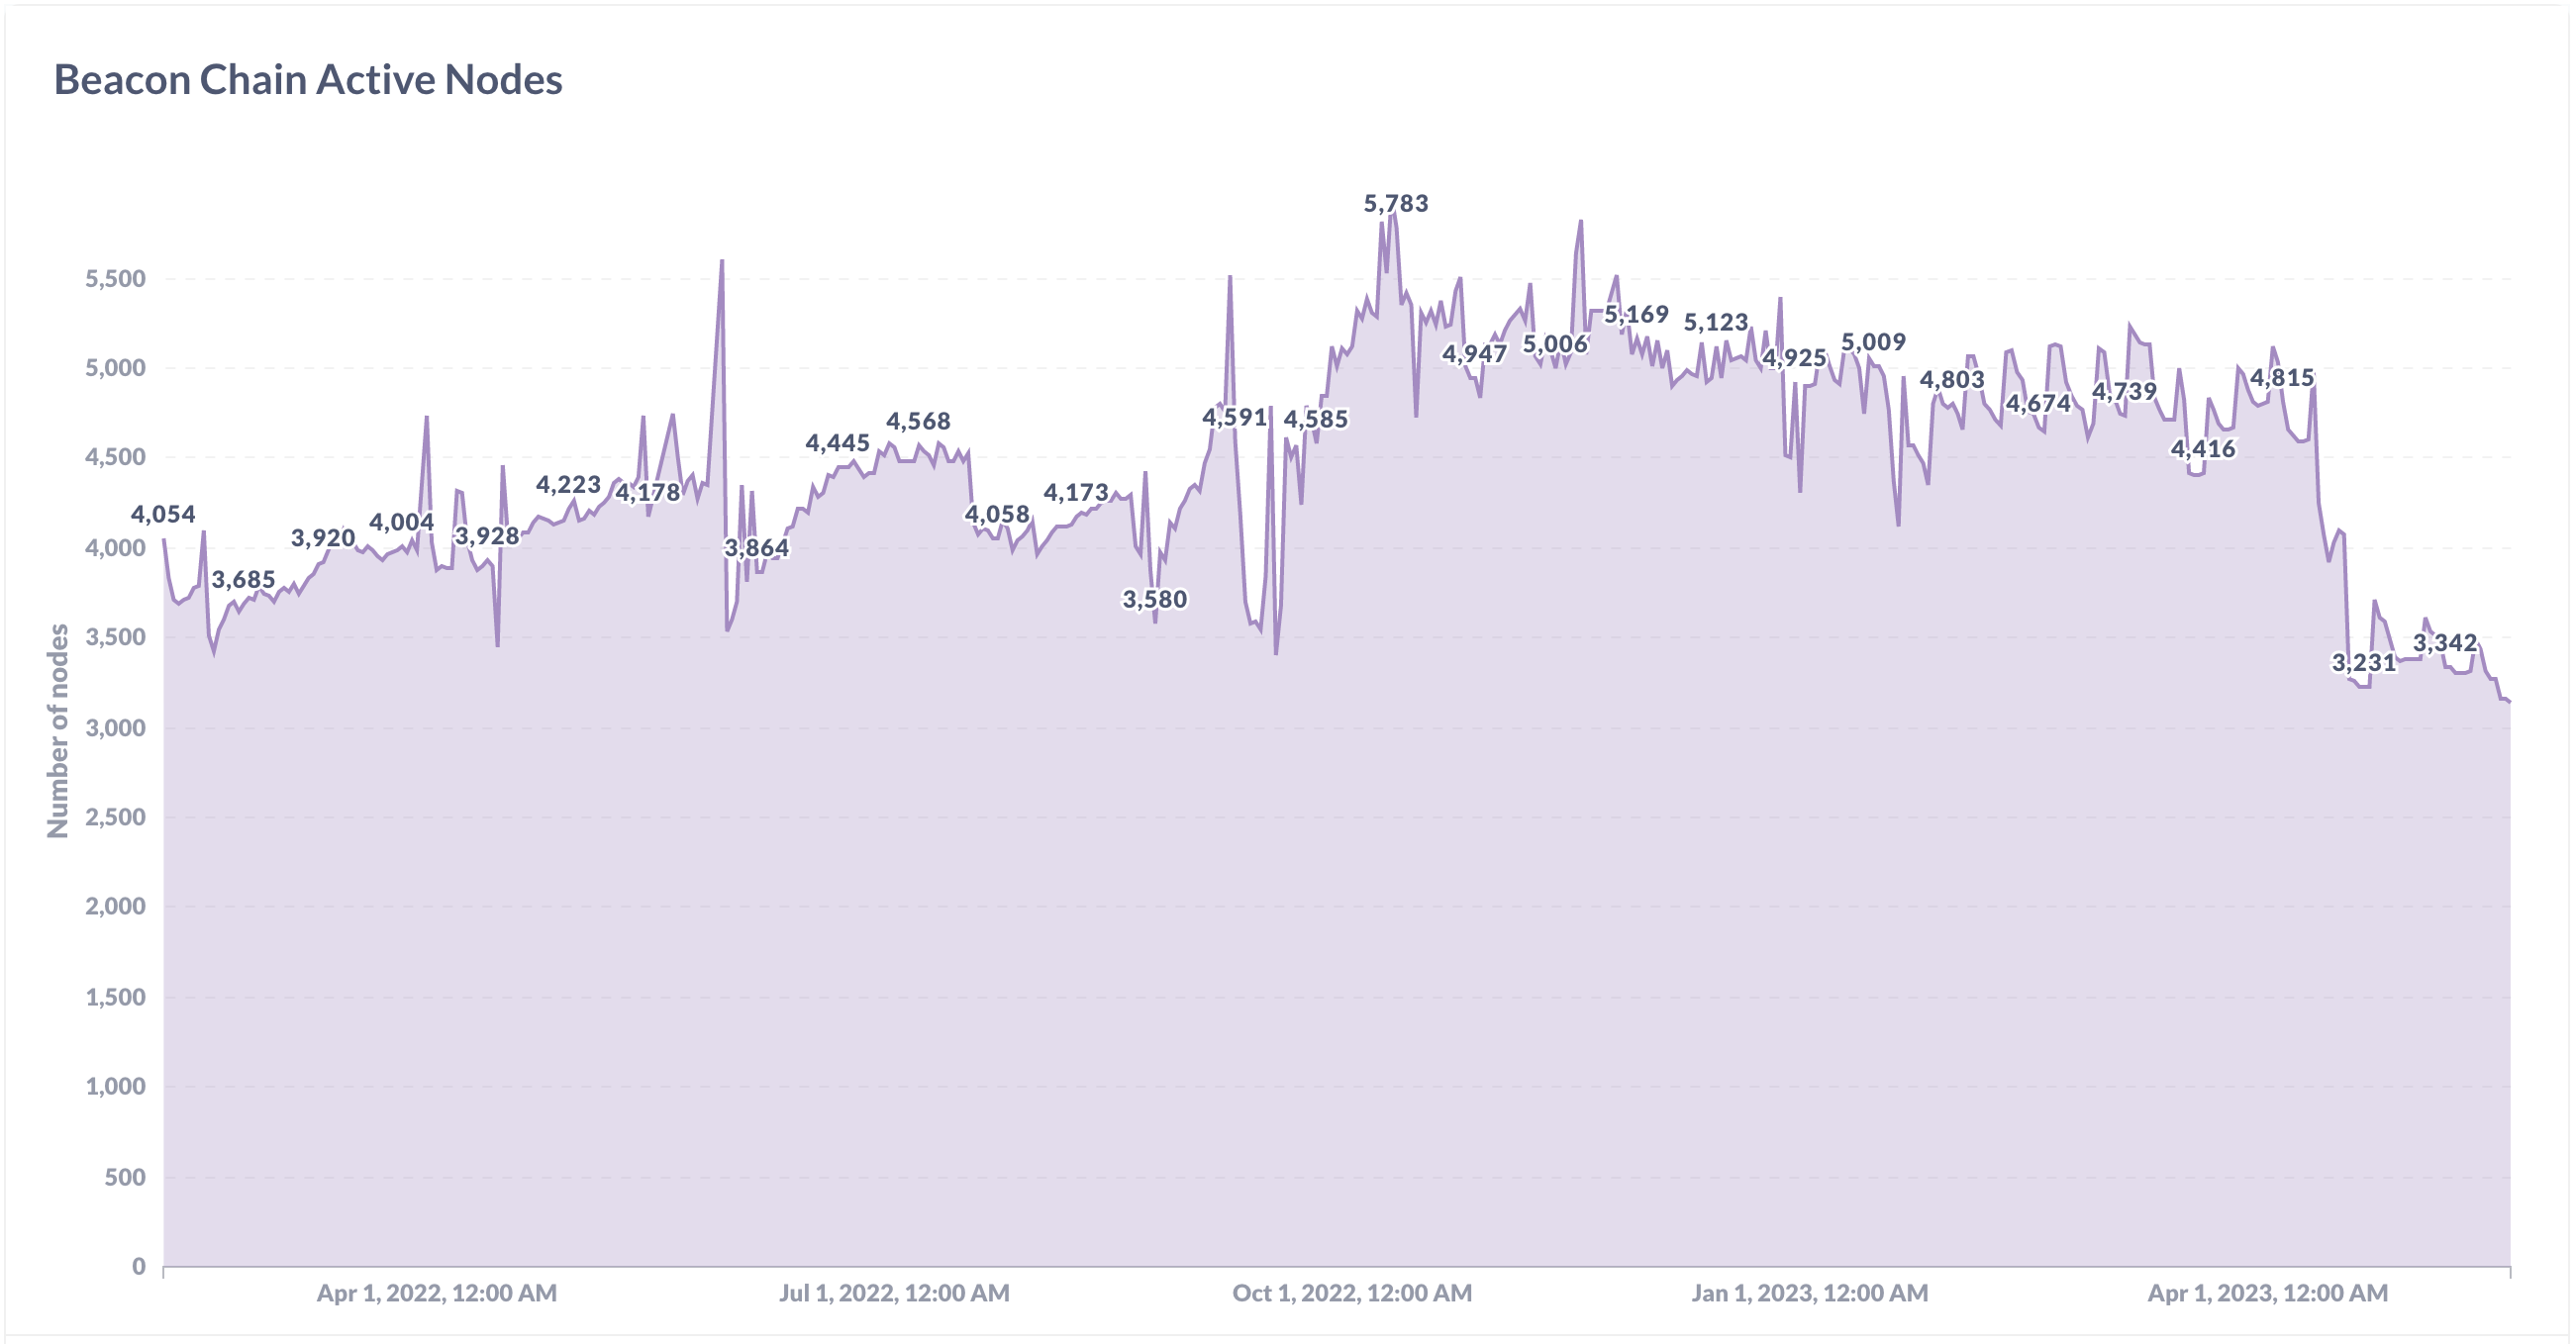
\includegraphics[width=0.48\linewidth]{images/activenodes}
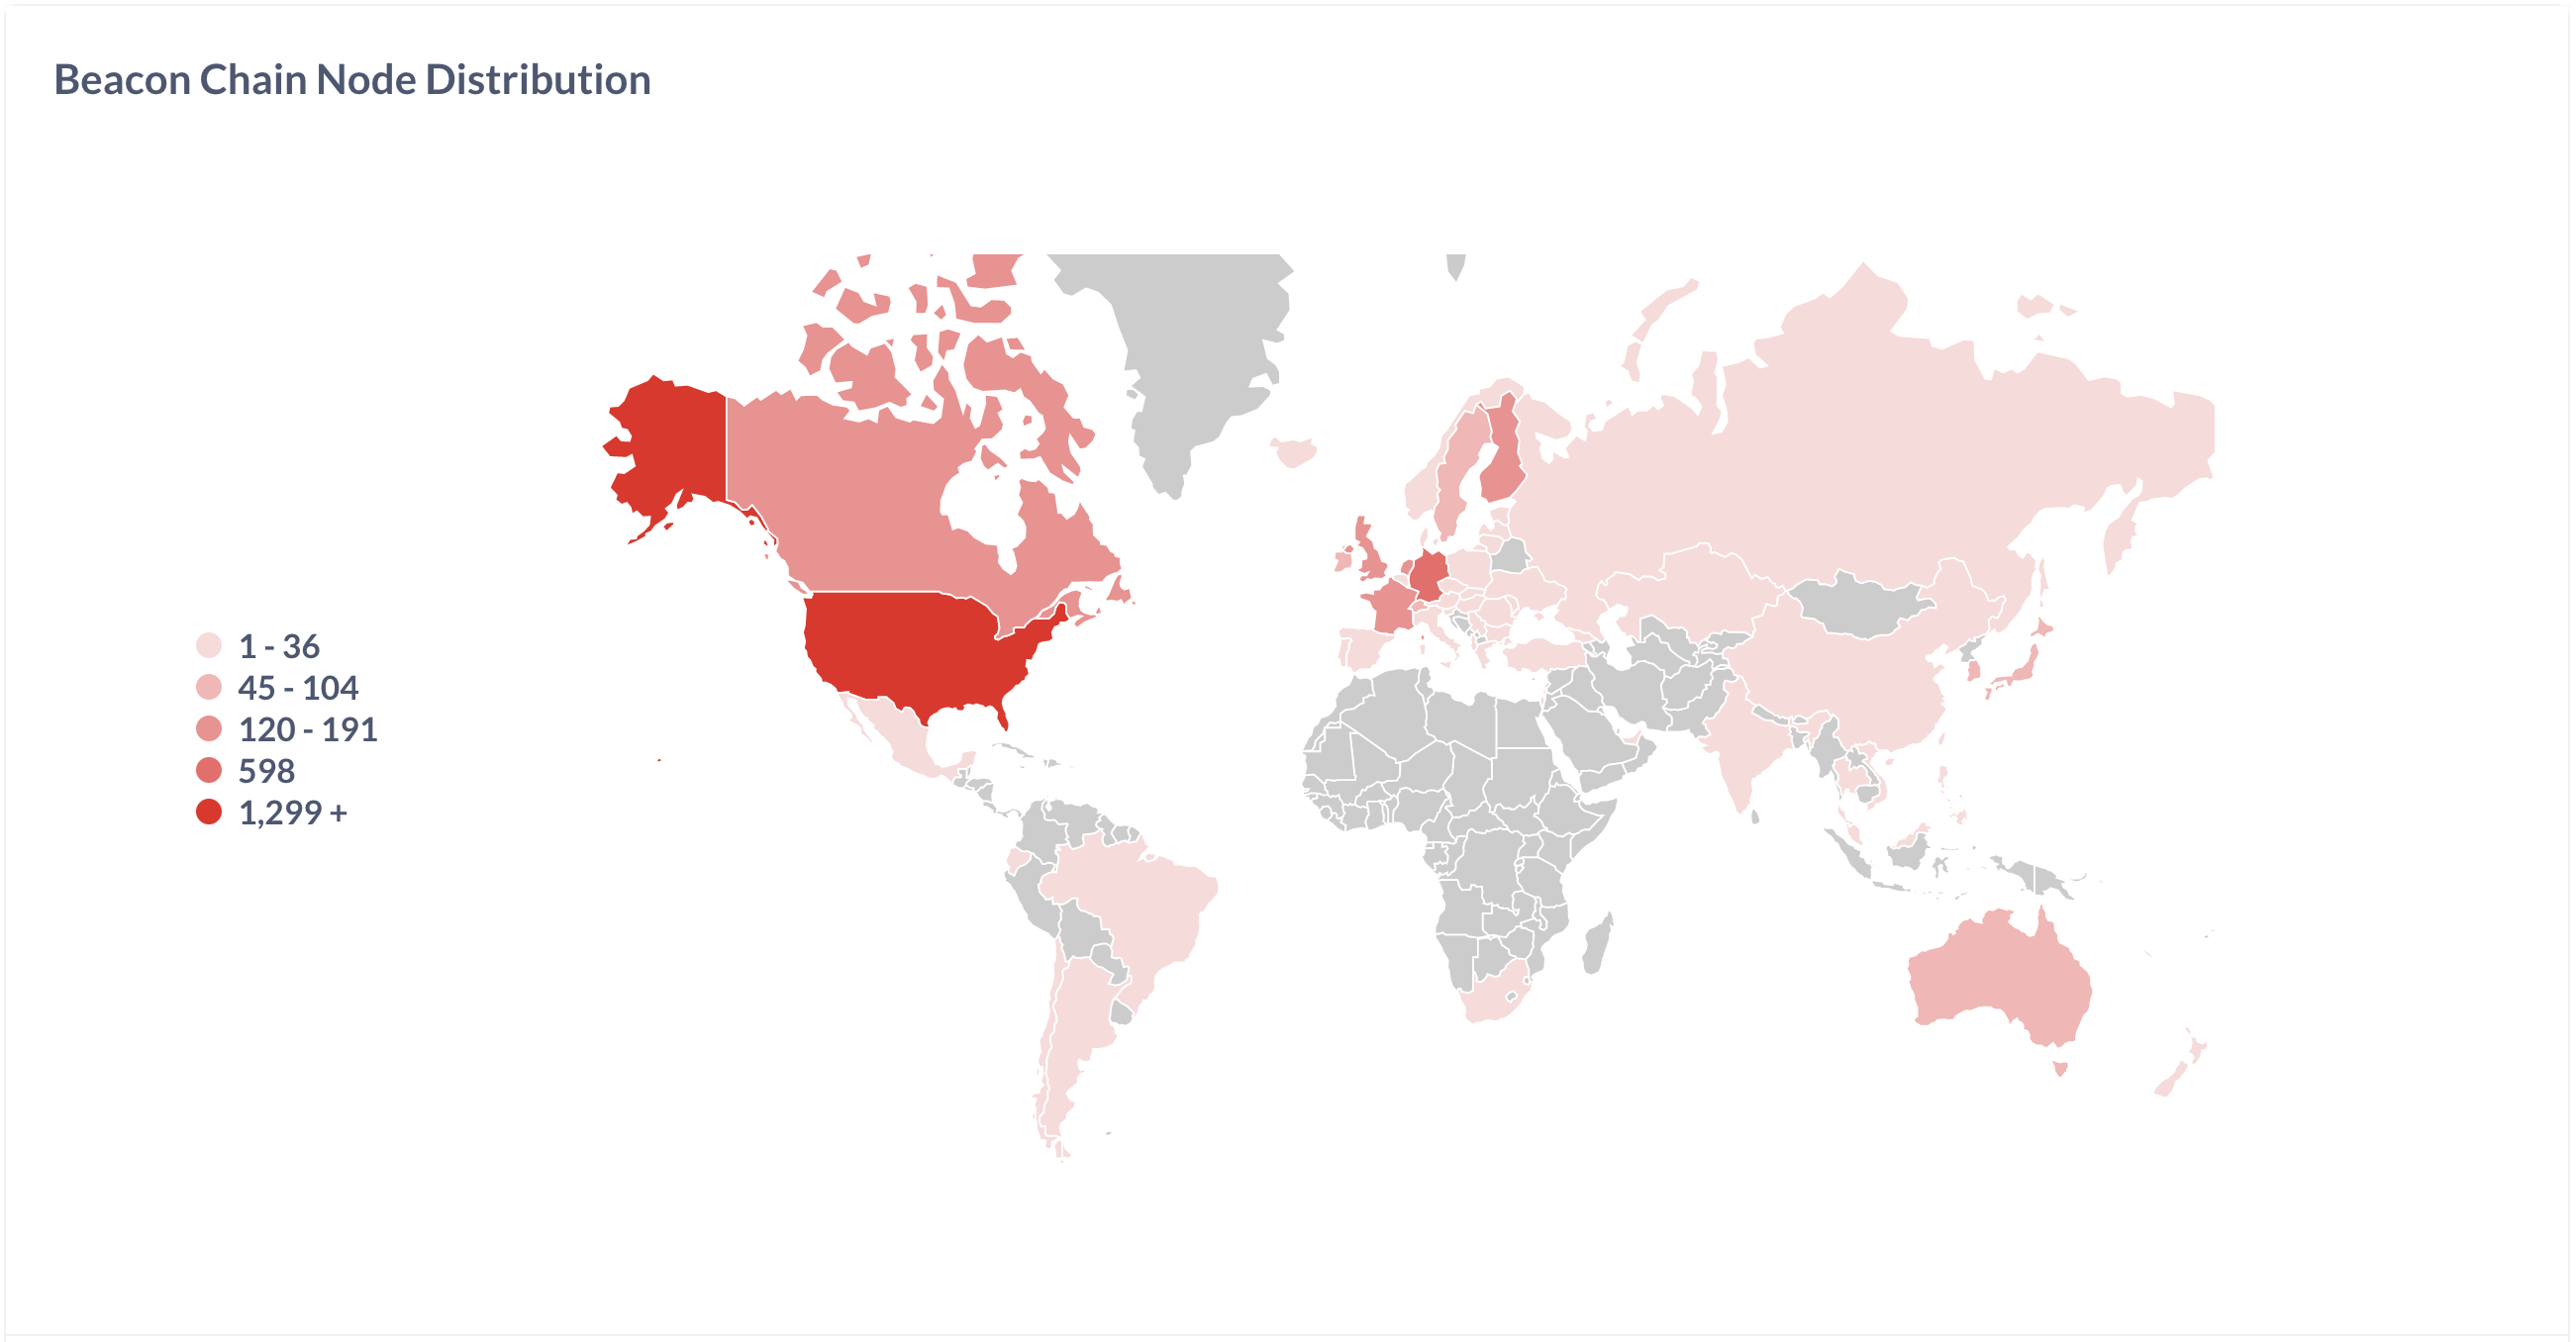
\includegraphics[width=0.48\linewidth]{images/evolution} \\
(a)\hspace{160pt}        (b)\\
\caption{Operating system distribution of active beacon chain nodes from Migalabs (a) and client diversity evolution of beacon chain nodes (b) (9 May 2023)}
\label{fig:active}
\end{center}
\end{figure}

\begin{figure}[htbp]
\begin{center}
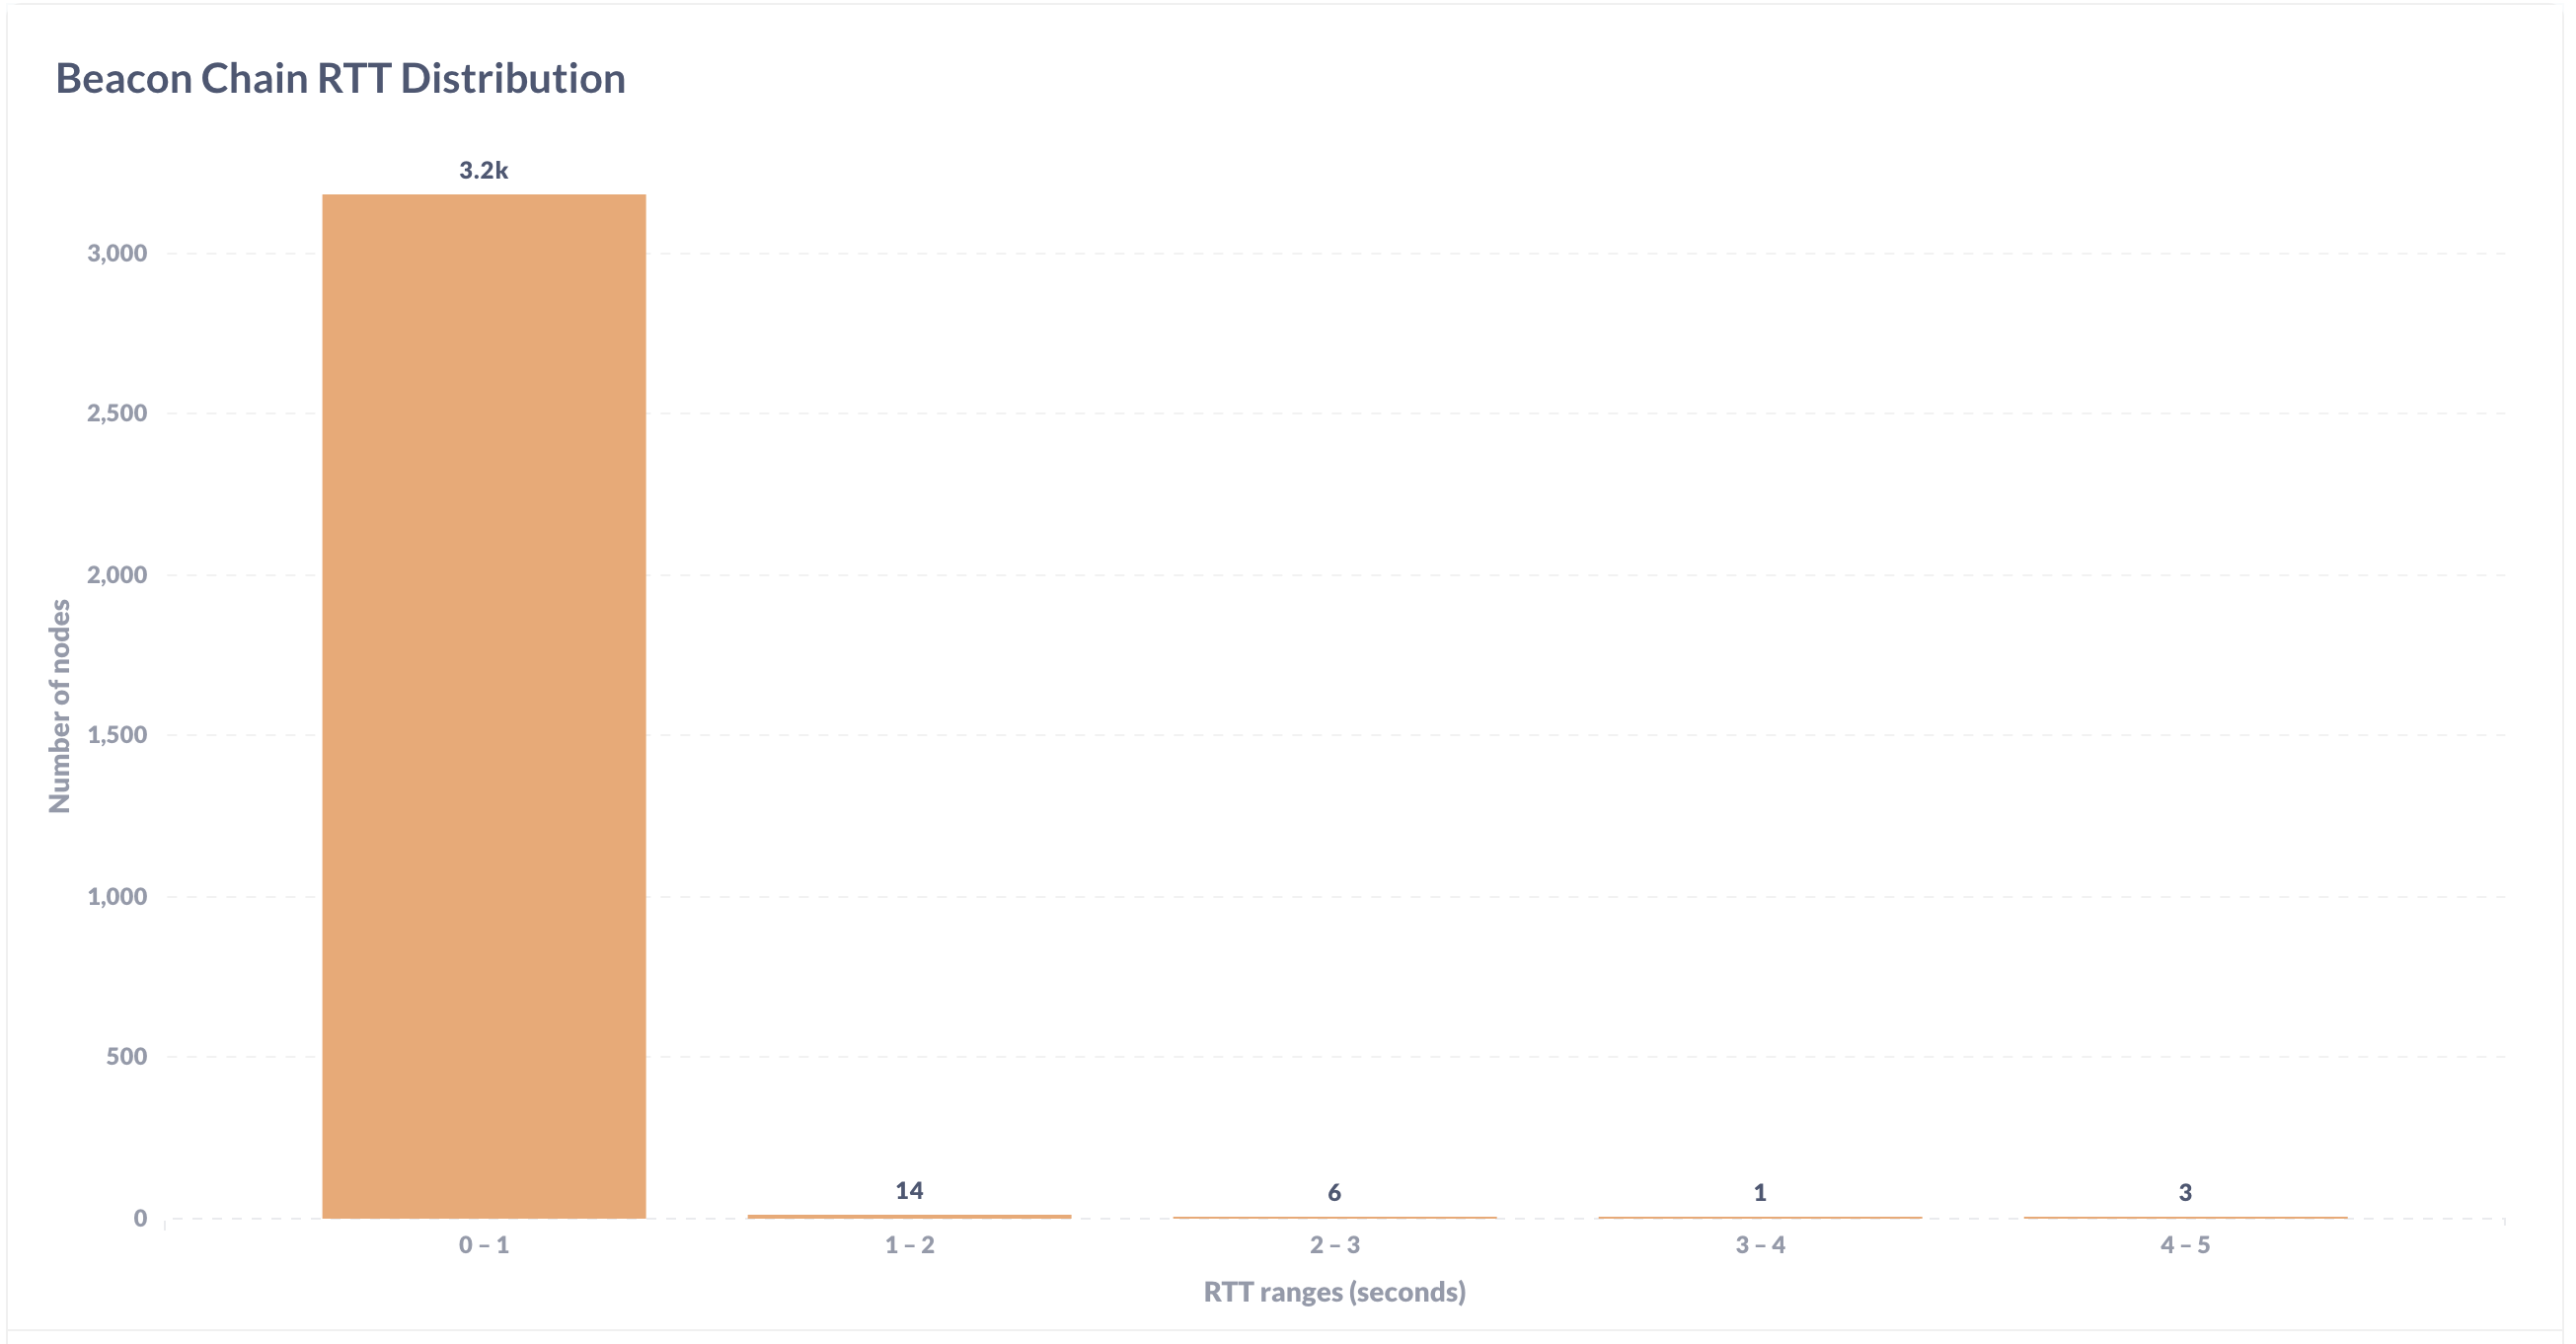
\includegraphics[width=0.48\linewidth]{images/activertt}
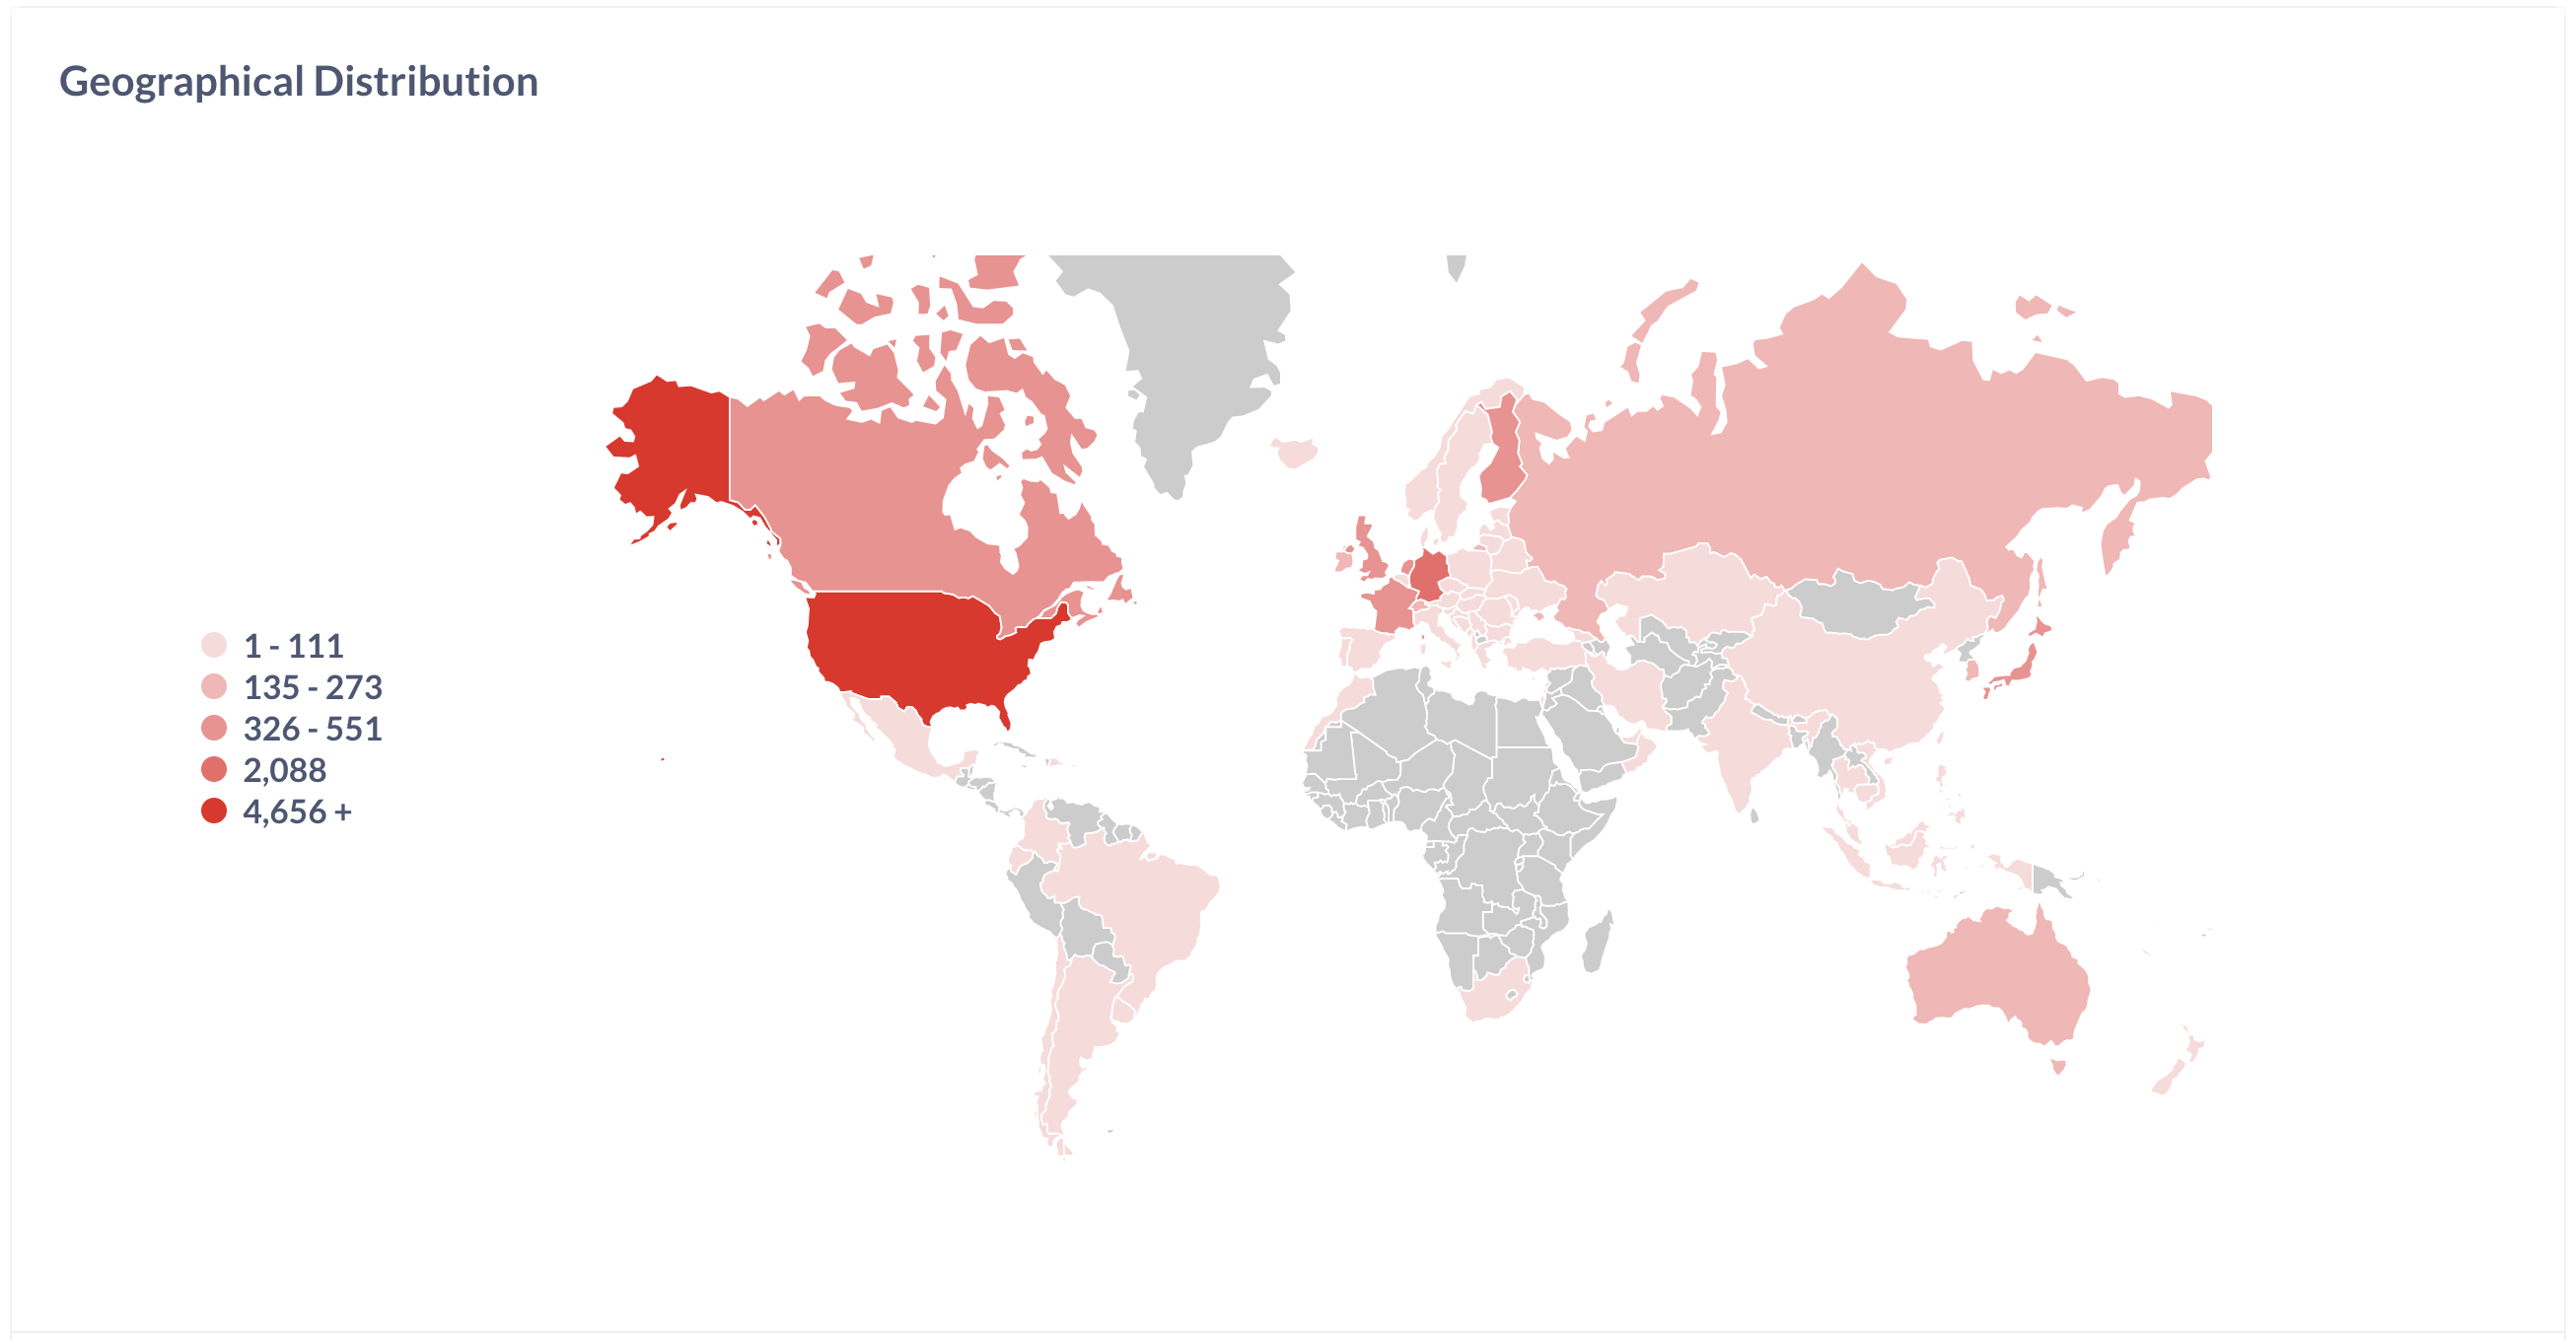
\includegraphics[width=0.48\linewidth]{images/geographical} \\
(a)\hspace{160pt}        (b)\\
\caption{Distribution of active beacon chain nodes round trip time (RTT) from Migalabs (a) and geographical distribution (b) (9 May 2023)}
\label{fig:rtt}
\end{center}
\end{figure}

\begin{figure}[htbp]
\begin{center}
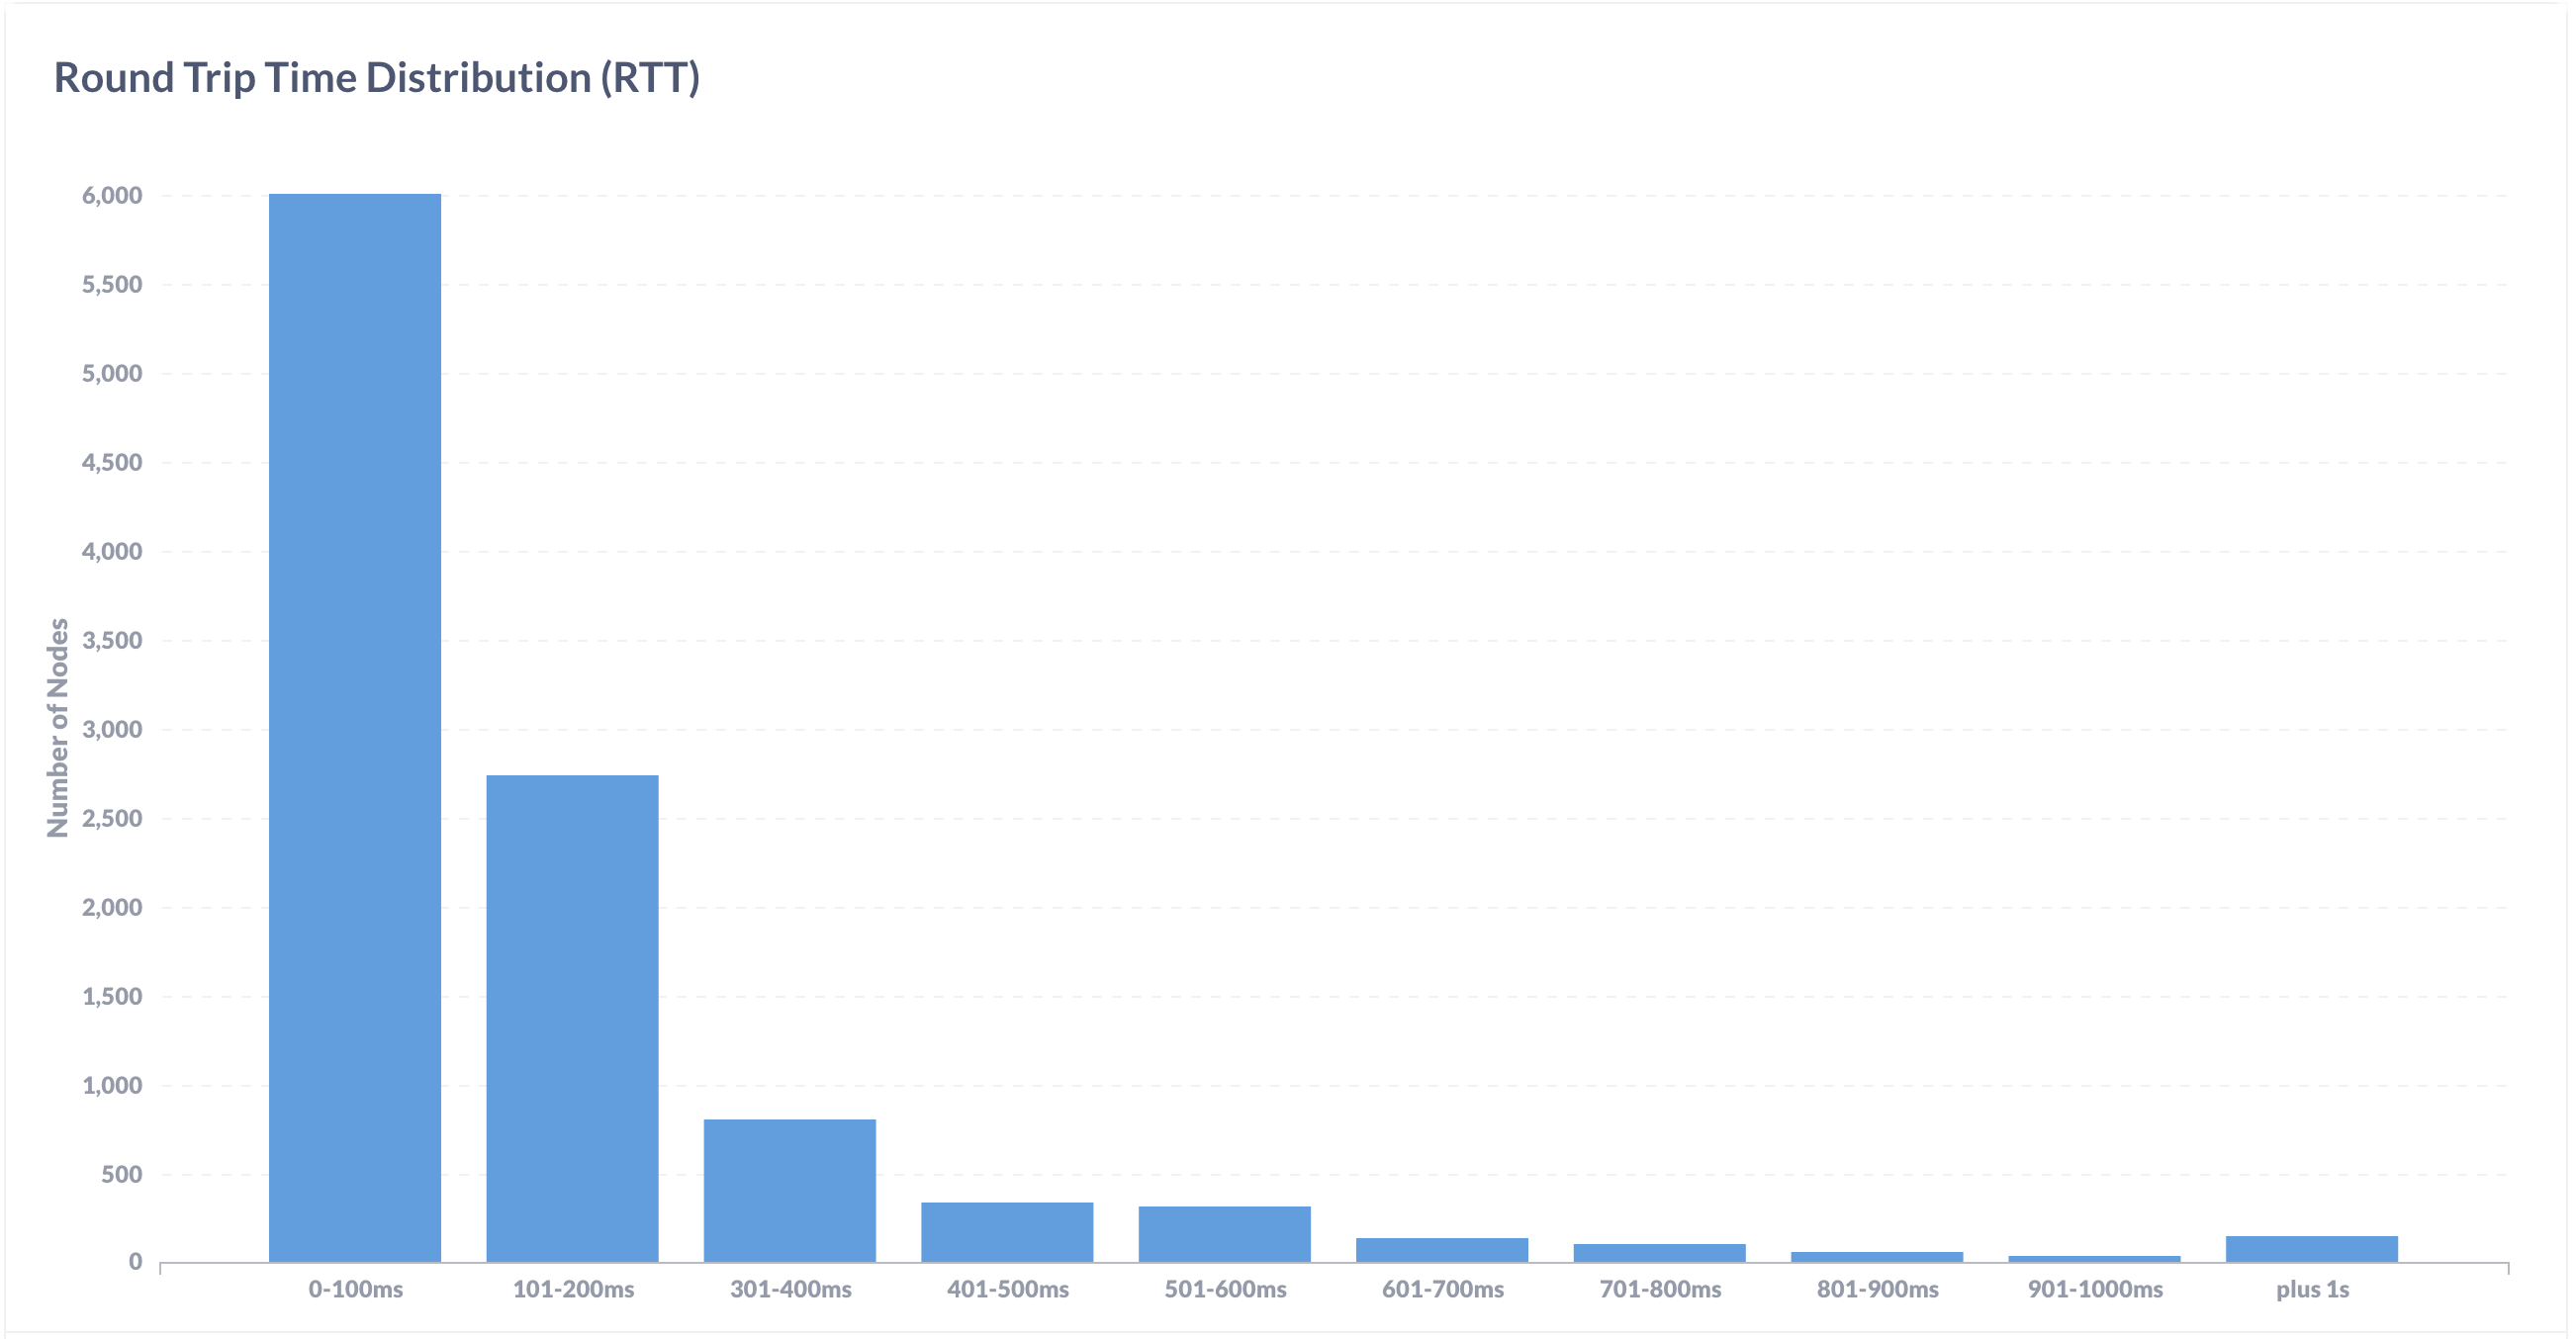
\includegraphics[width=0.48\linewidth]{images/rttdist}
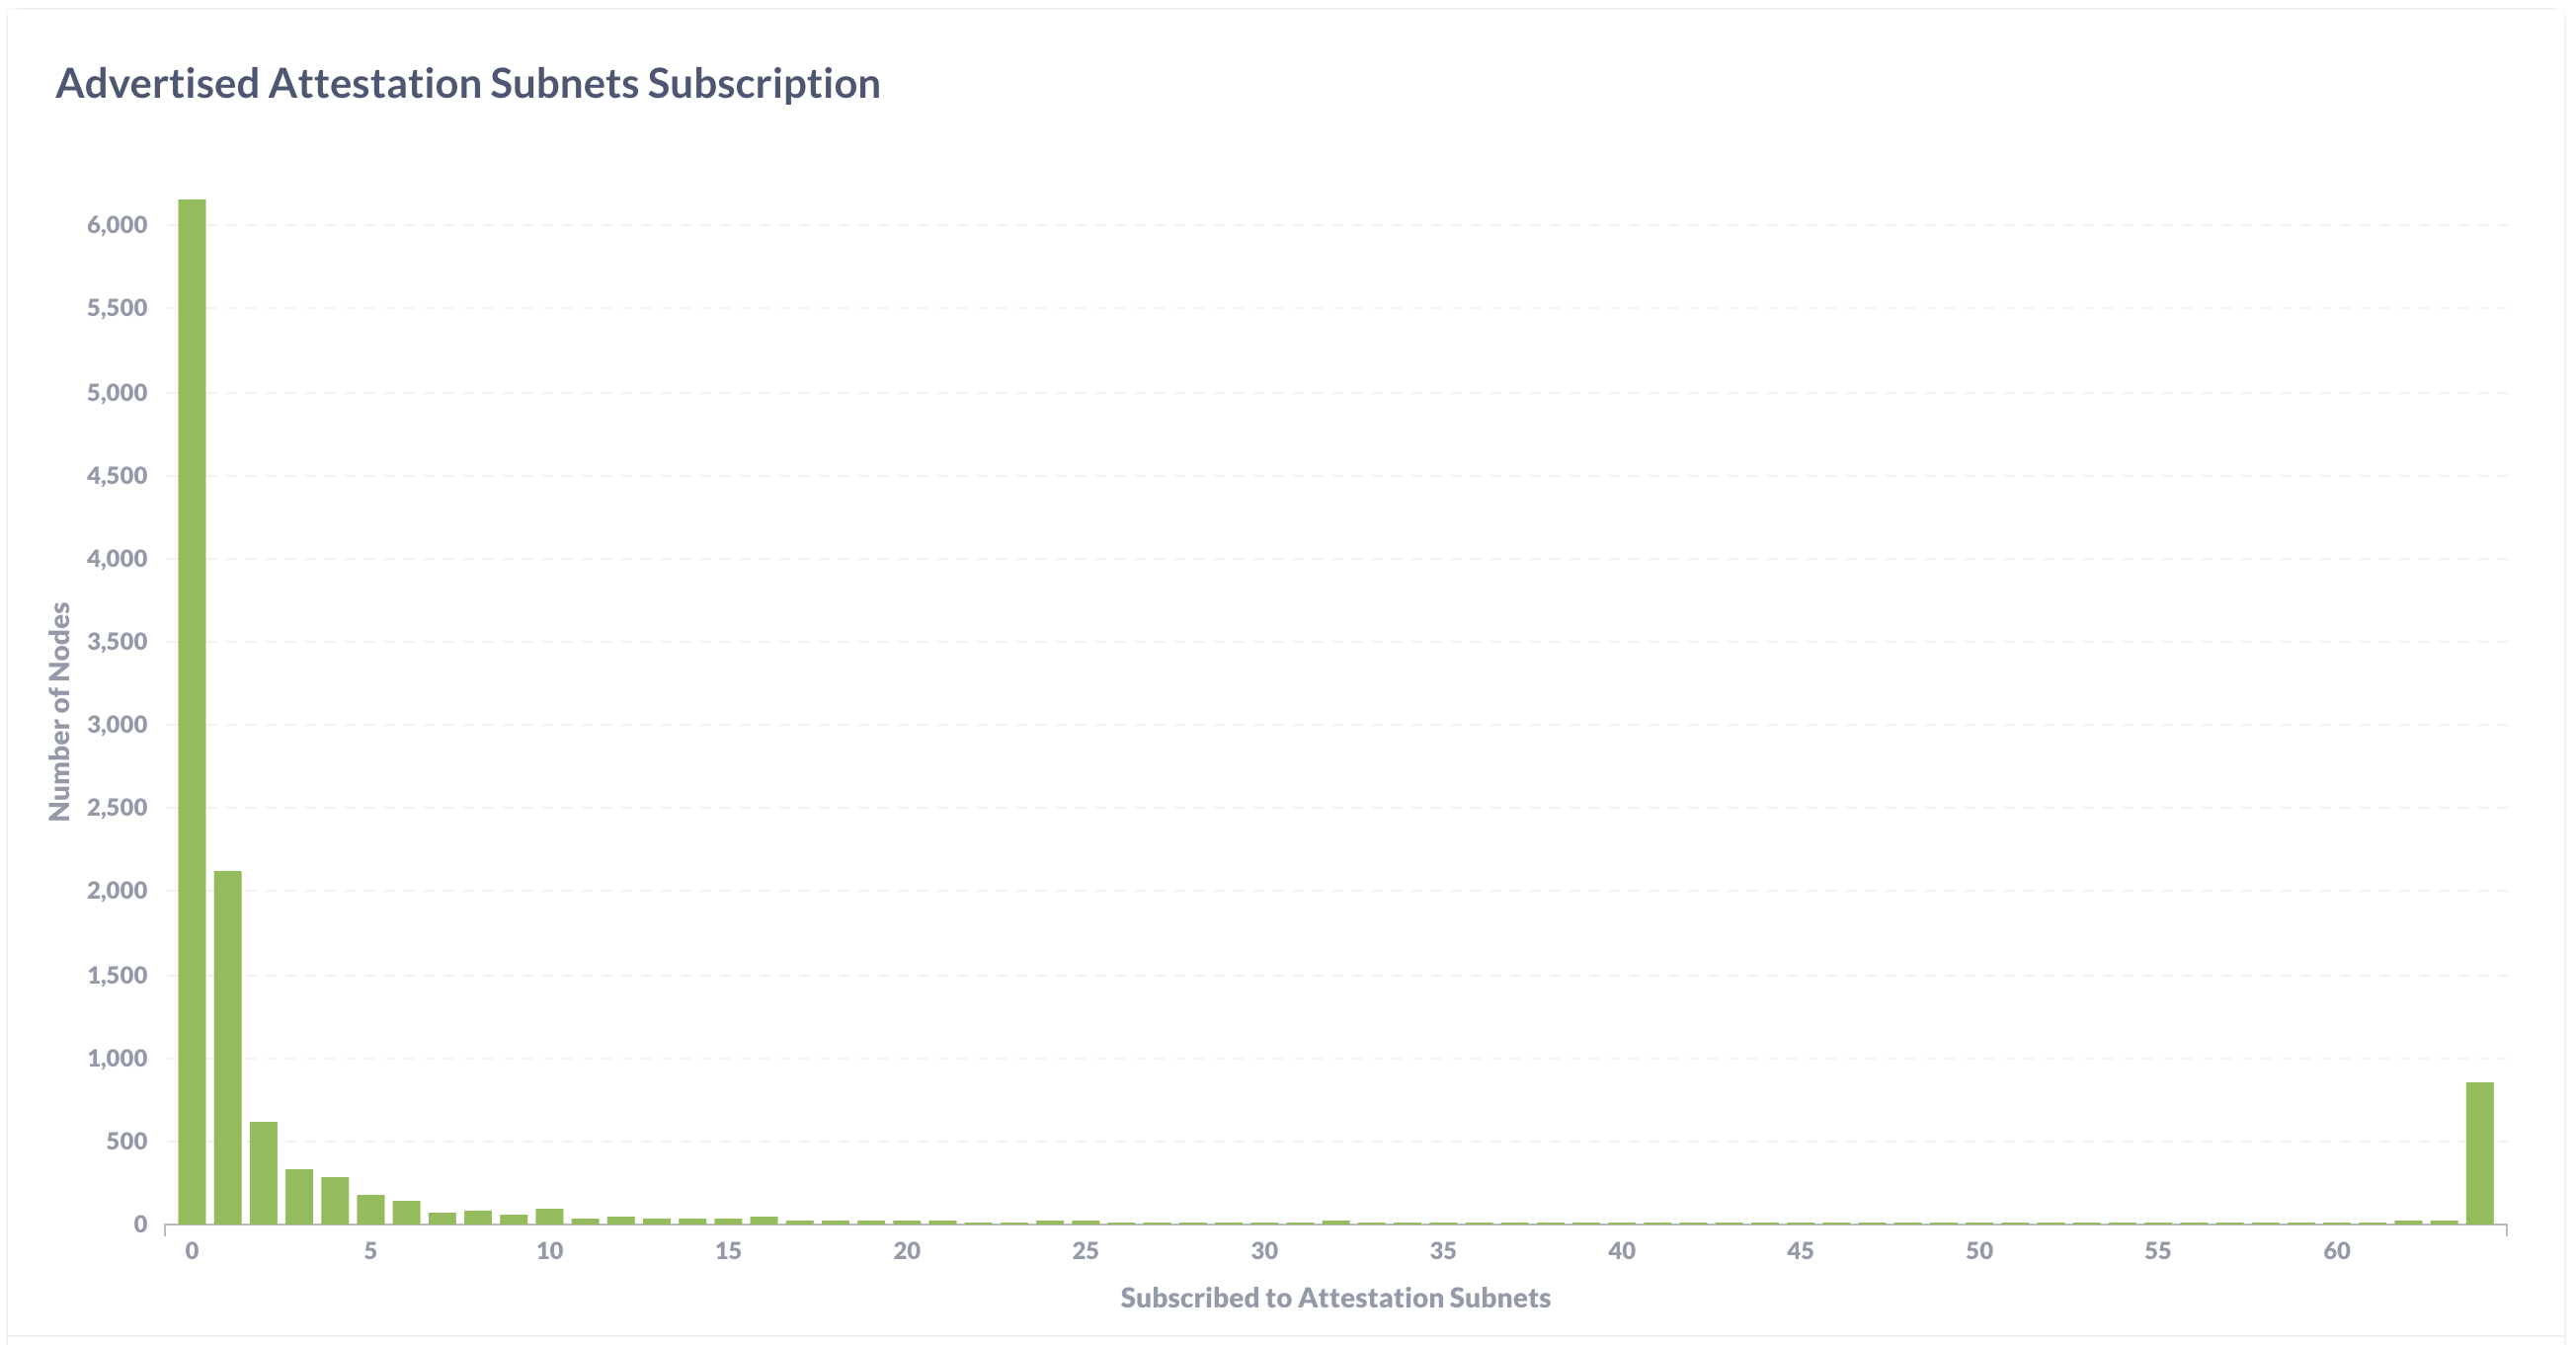
\includegraphics[width=0.48\linewidth]{images/aass} \\
(a)\hspace{160pt}        (b)\\
\caption{Distribution of active beacon chain nodes round trip time distribution (RTT) from Migalabs (a) and advertised attestation subnets subscription (b) (9 May 2023)}
\label{fig:aass}
\end{center}
\end{figure}

\begin{figure}[htbp]
\begin{center}
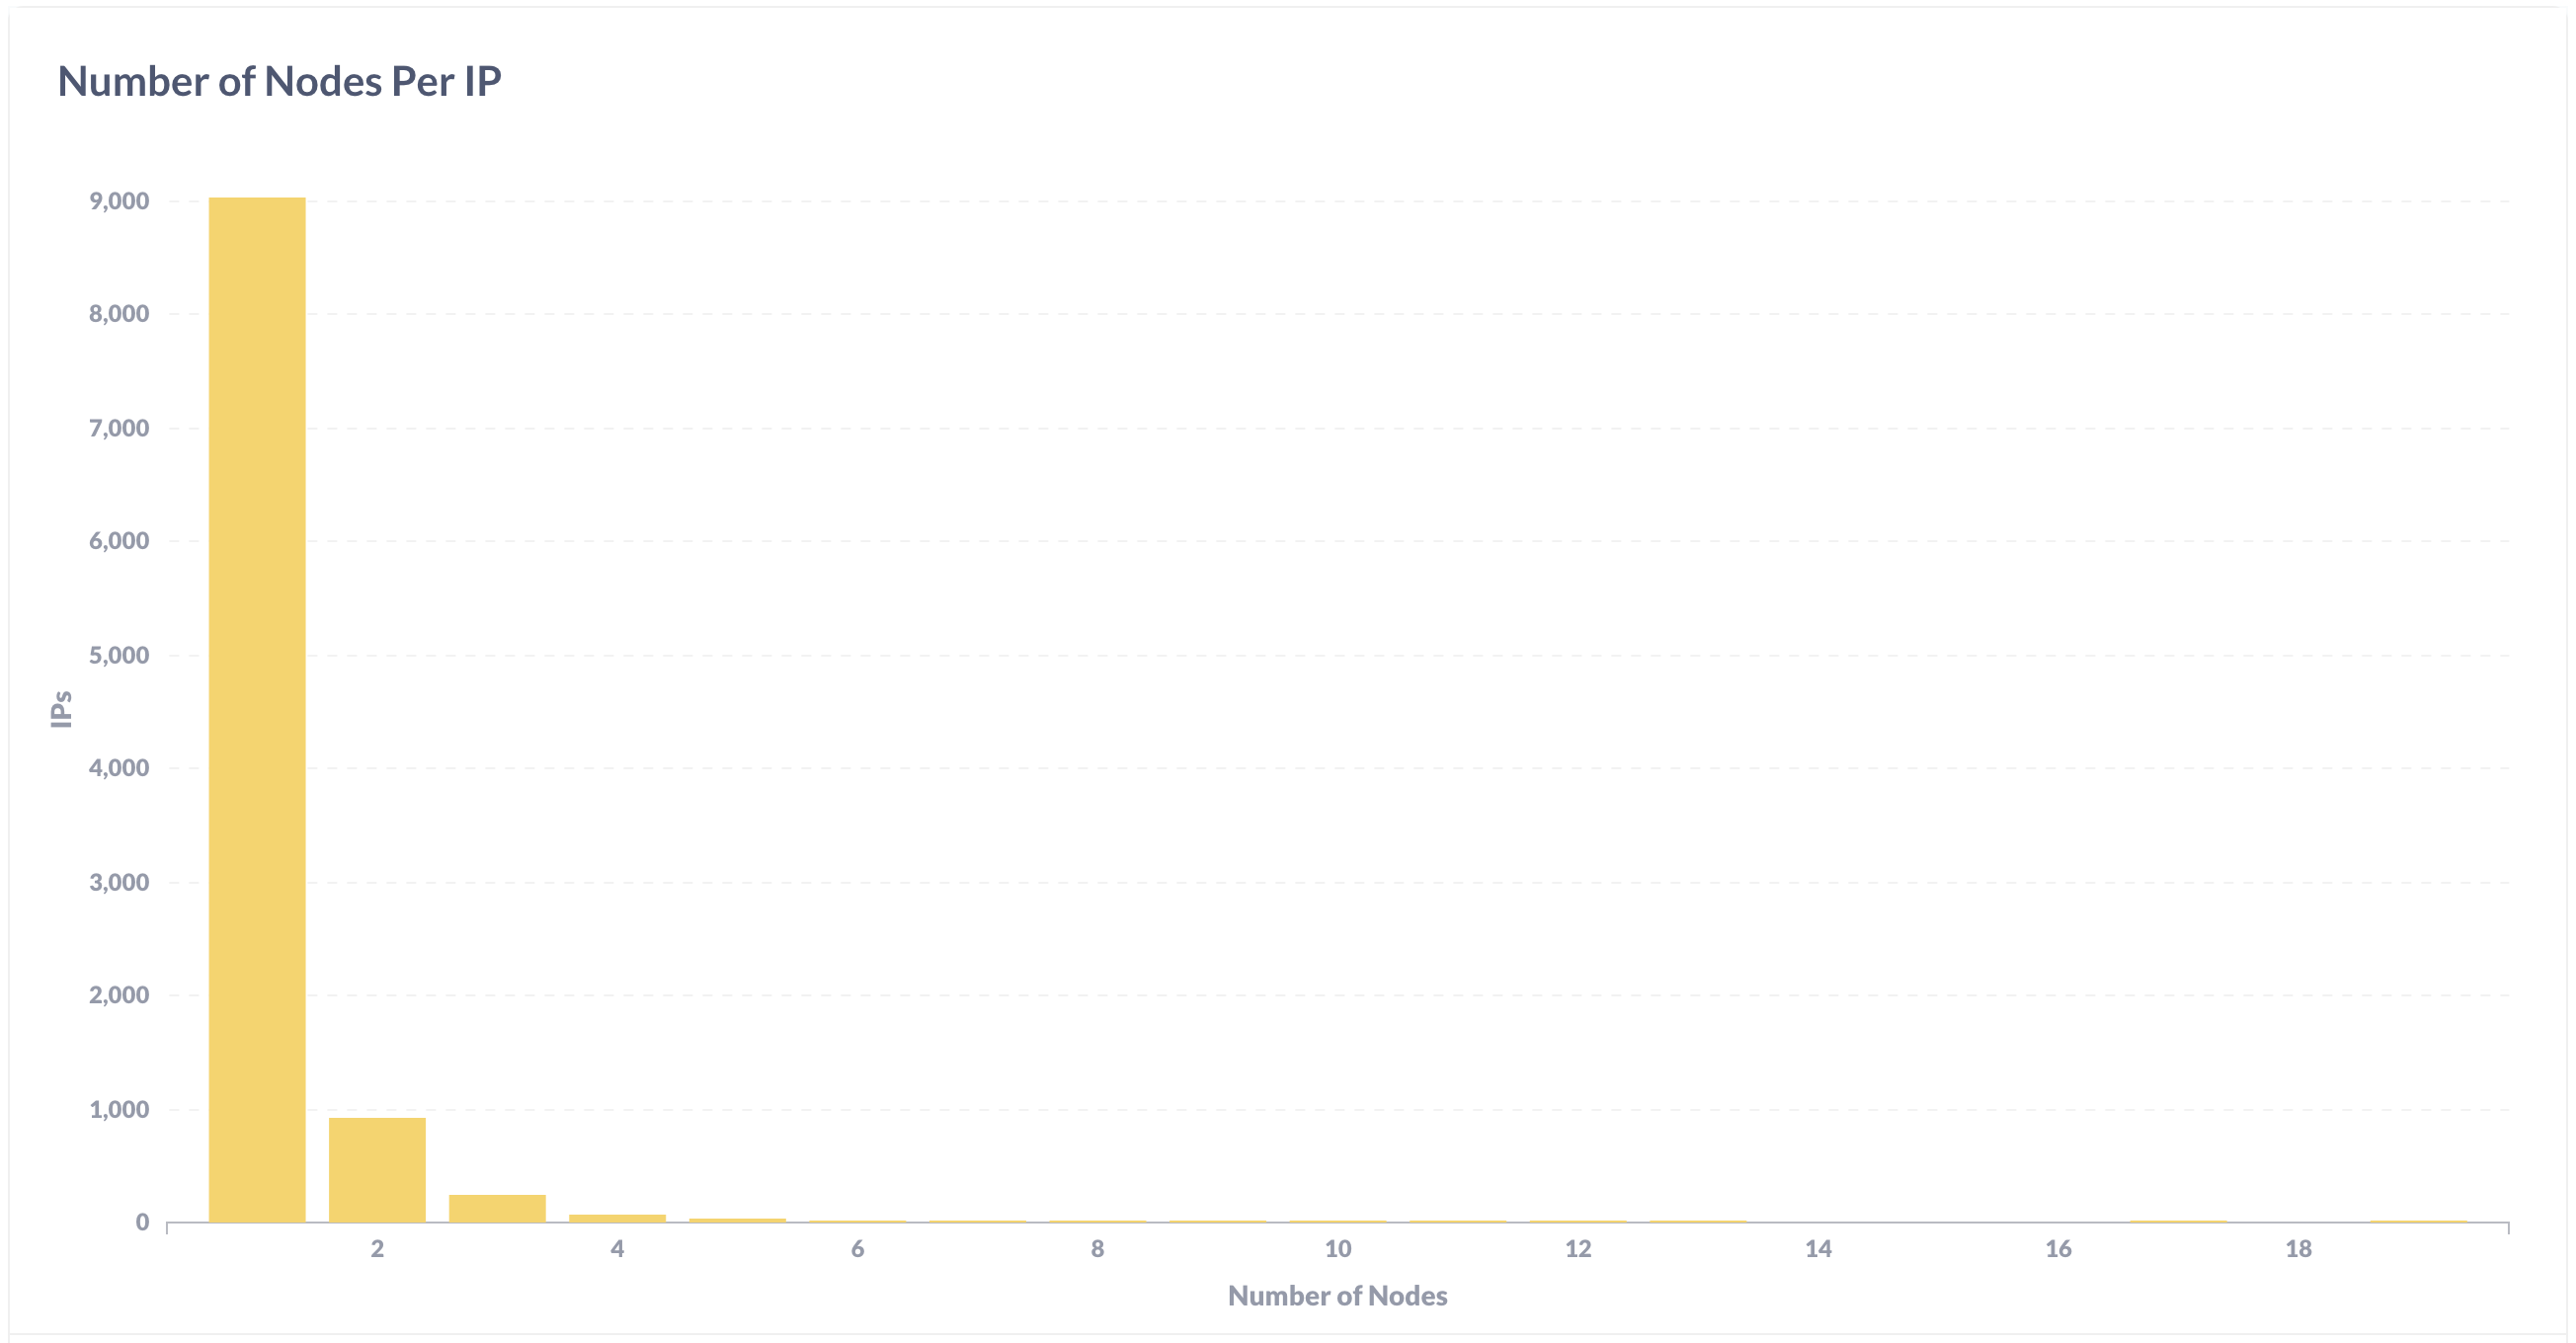
\includegraphics[width=0.48\linewidth]{images/ipdist}
\caption{Number of beacon nodes per IP from Migalabs }
\label{fig:ipdist}
\end{center}
\end{figure}
\clearpage
% --------------------------------------
\subsubsection*{Ultrasound money}
% --------------------------------------

\begin{figure}[htbp]
\begin{center}
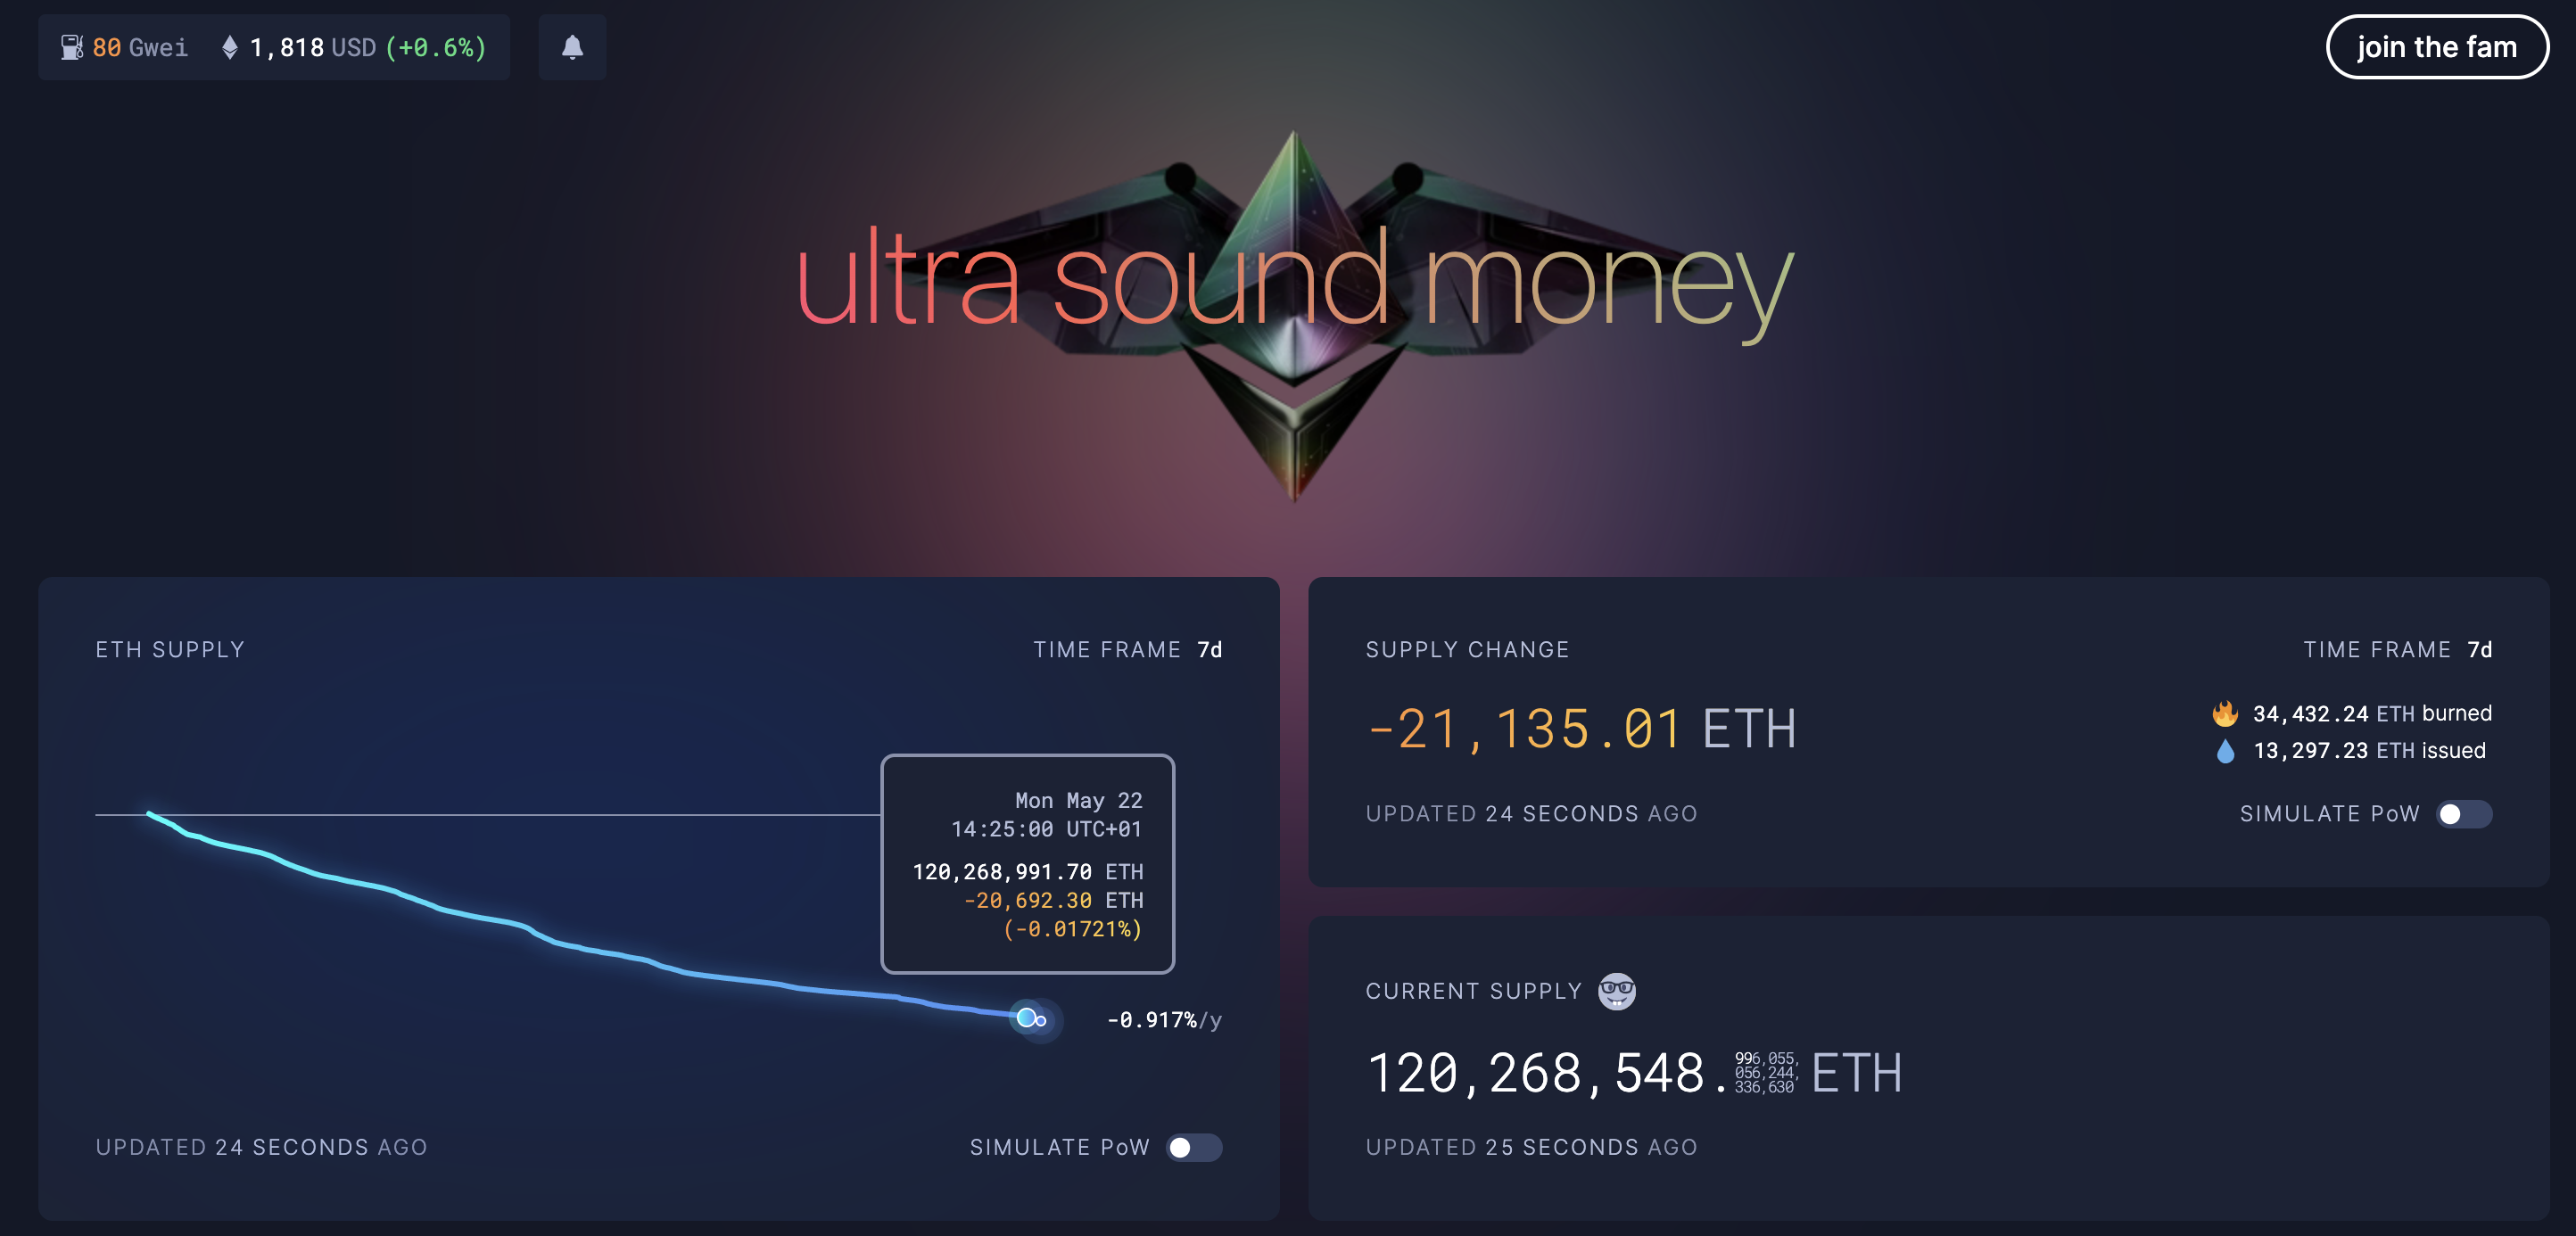
\includegraphics[width=0.9\linewidth]{images/ethsupply}
\caption{ETH supply over time, current supply and change, 22 May 2023}
\label{fig:ethsupply}
\end{center}
\end{figure}

\begin{figure}[htbp]
\begin{center}
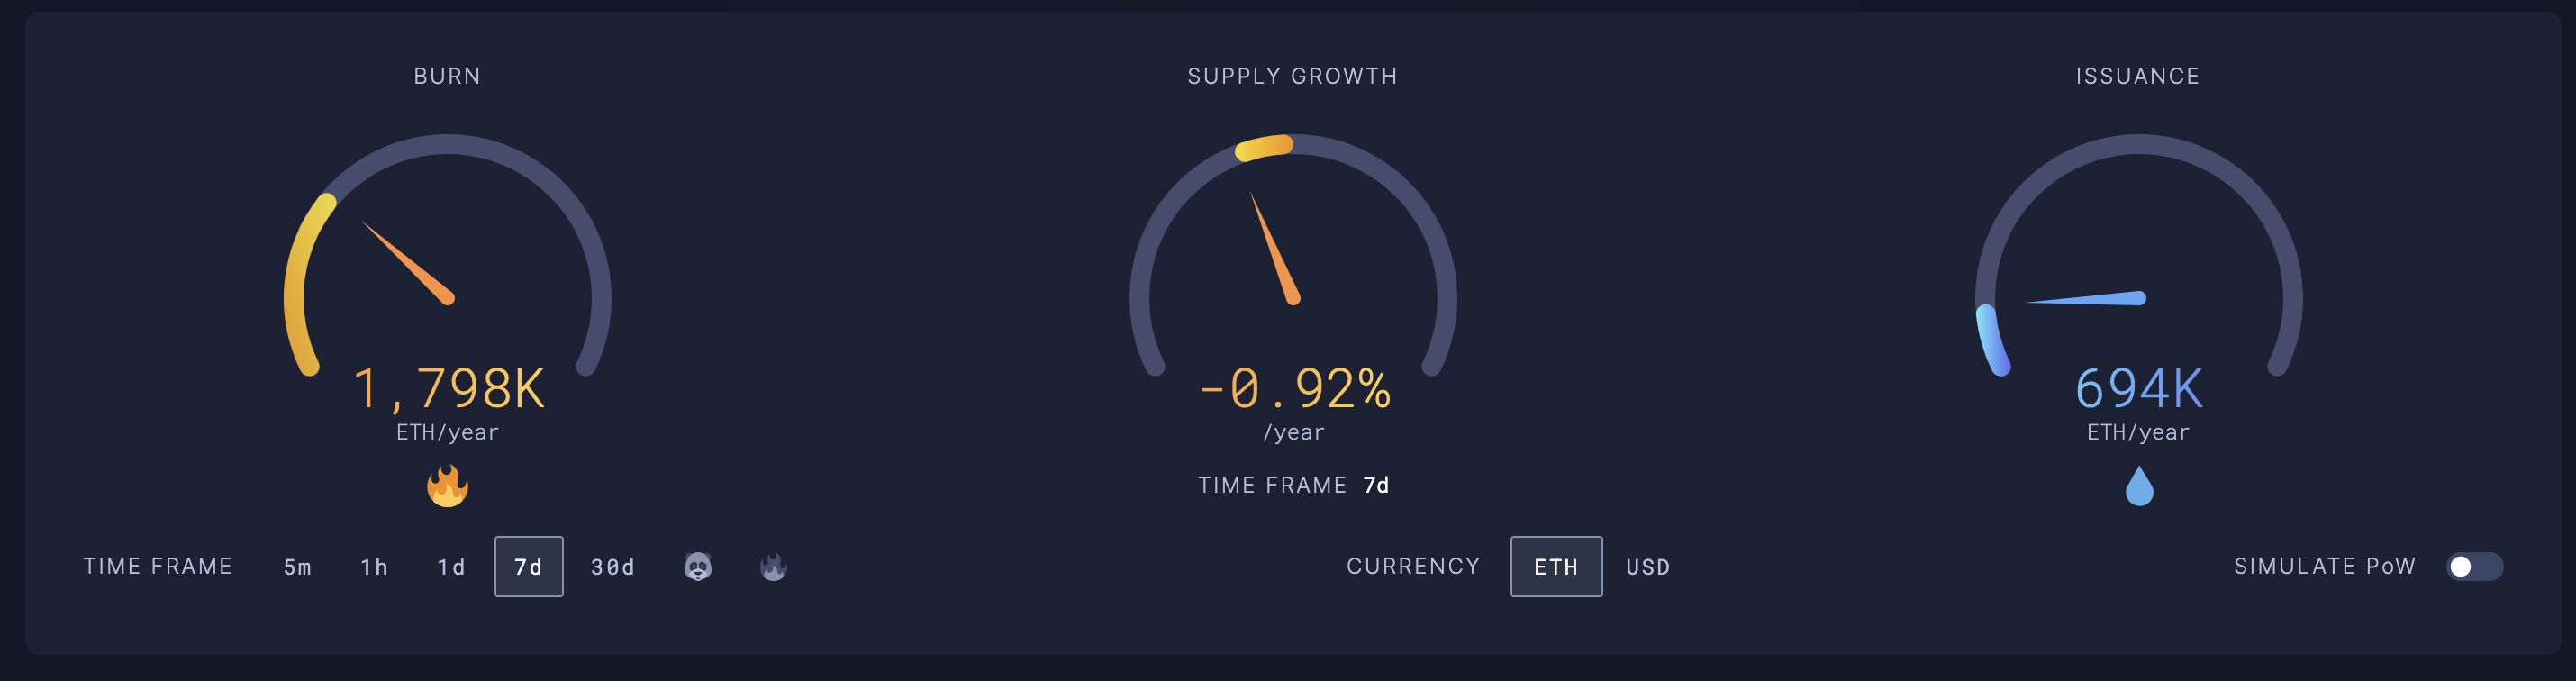
\includegraphics[width=0.9\linewidth]{images/burn}
\caption{Burn, supply growth, and issuance, 22 May 2023}
\label{fig:burn}
\end{center}
\end{figure}

\begin{figure}[htbp]
\begin{center}
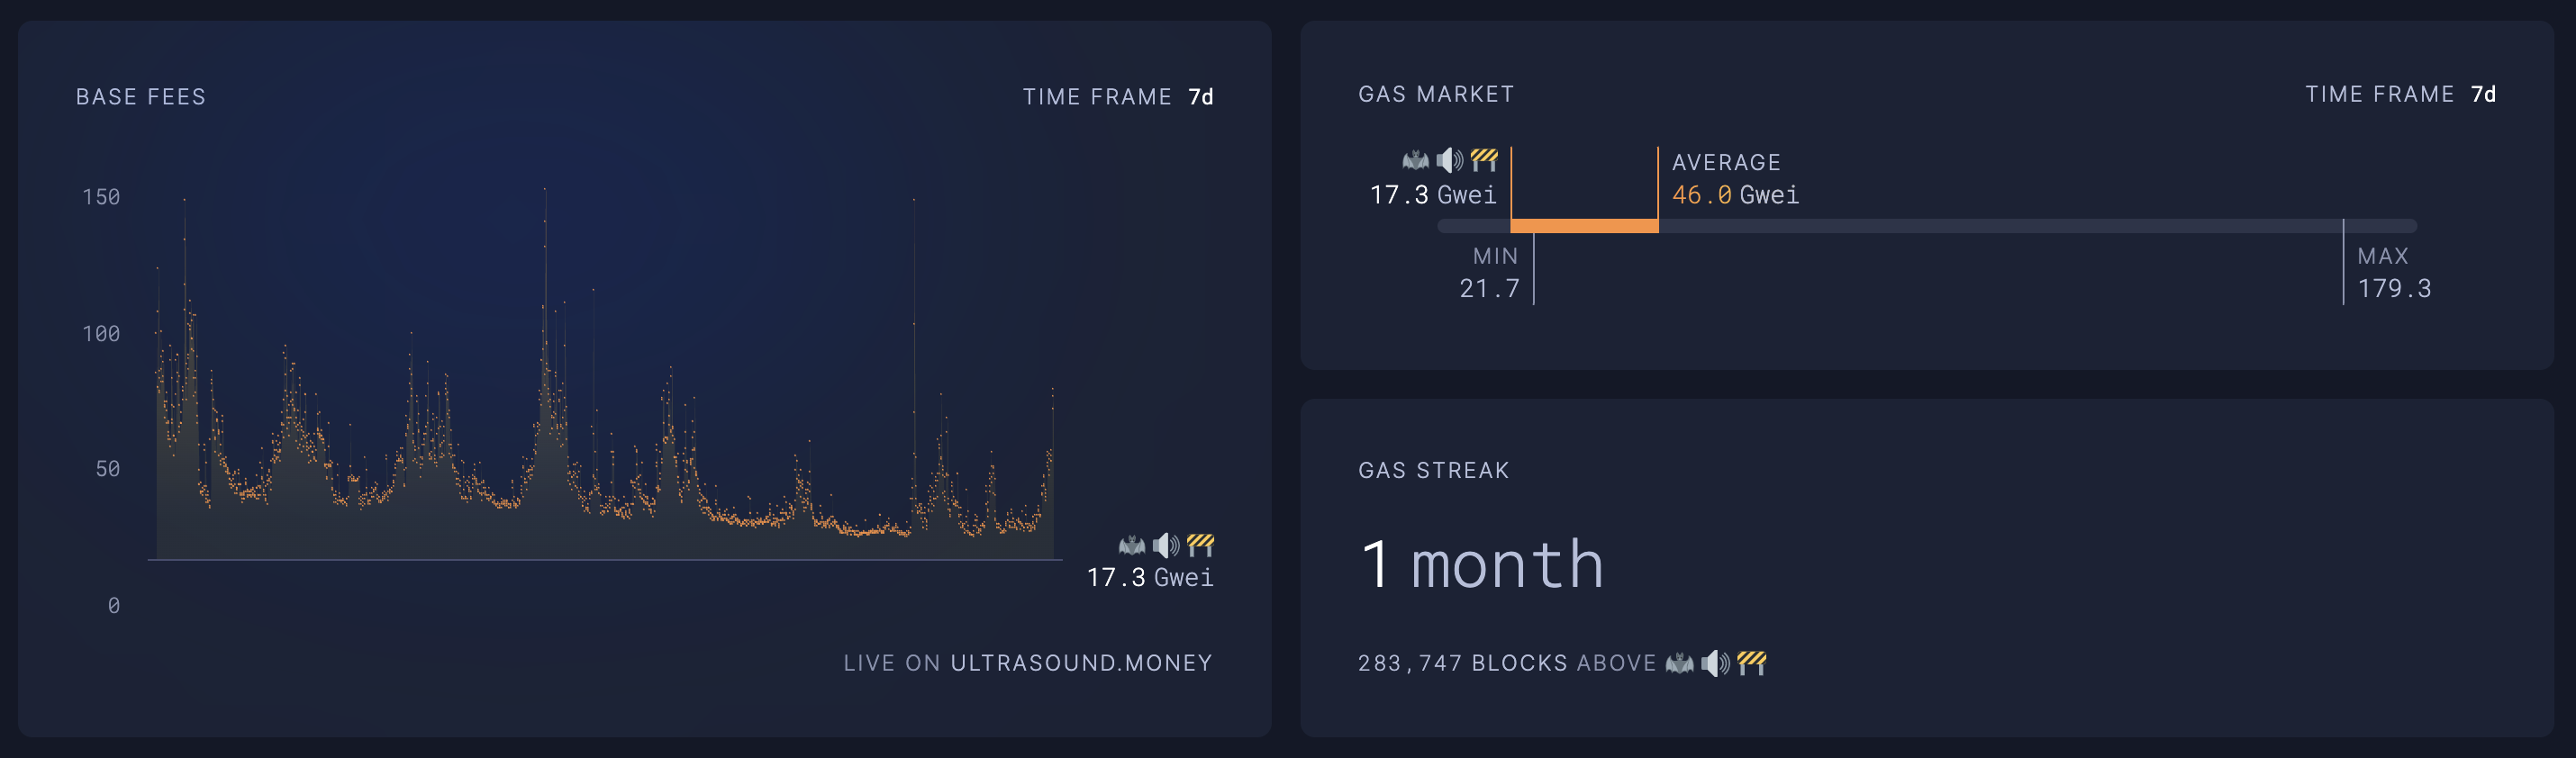
\includegraphics[width=0.9\linewidth]{images/gasmarket}
\caption{Gas market, 22 May 2023}
\label{fig:gas}
\end{center}
\end{figure}

\begin{figure}[htbp]
\begin{center}
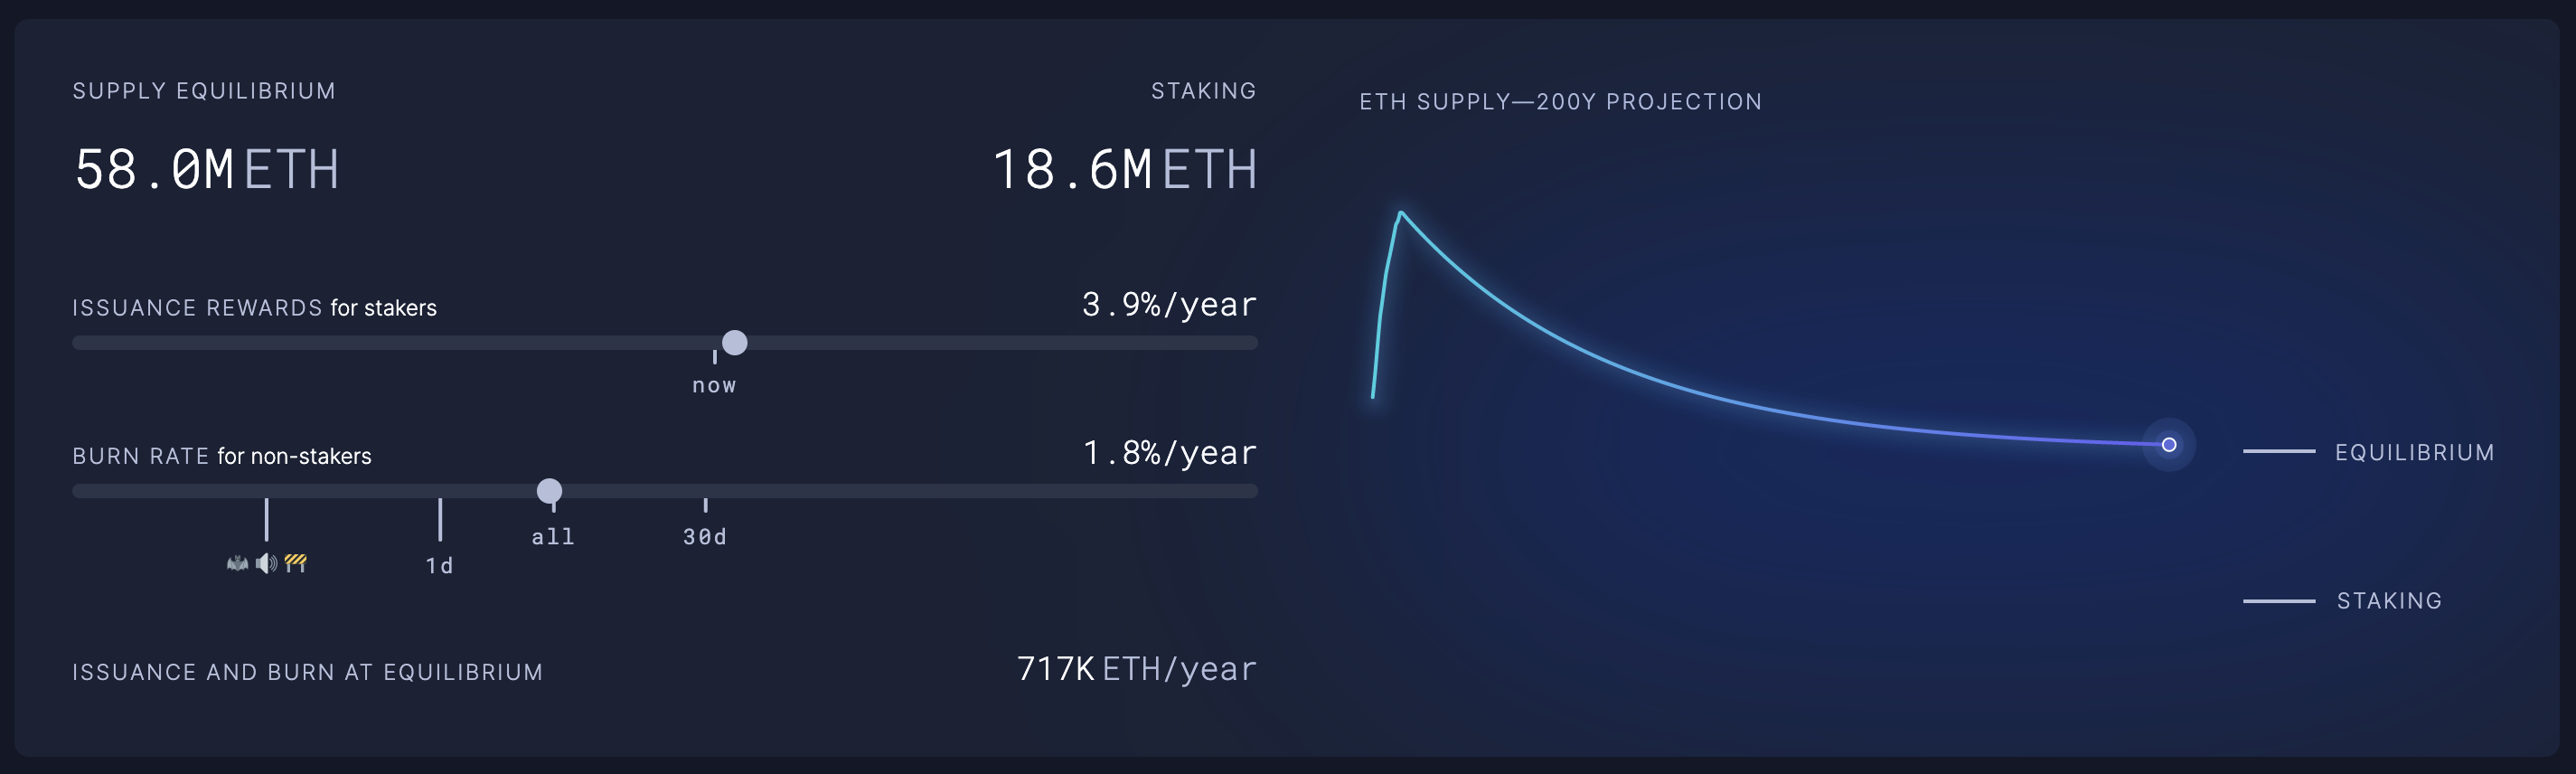
\includegraphics[width=0.9\linewidth]{images/projection}
\caption{Interactive ETH supply projections - sliders provided for issuance rewards and burn rate , 22 May 2023}
\label{fig:projection}
\end{center}
\end{figure}

\begin{figure}[htbp]
\begin{center}
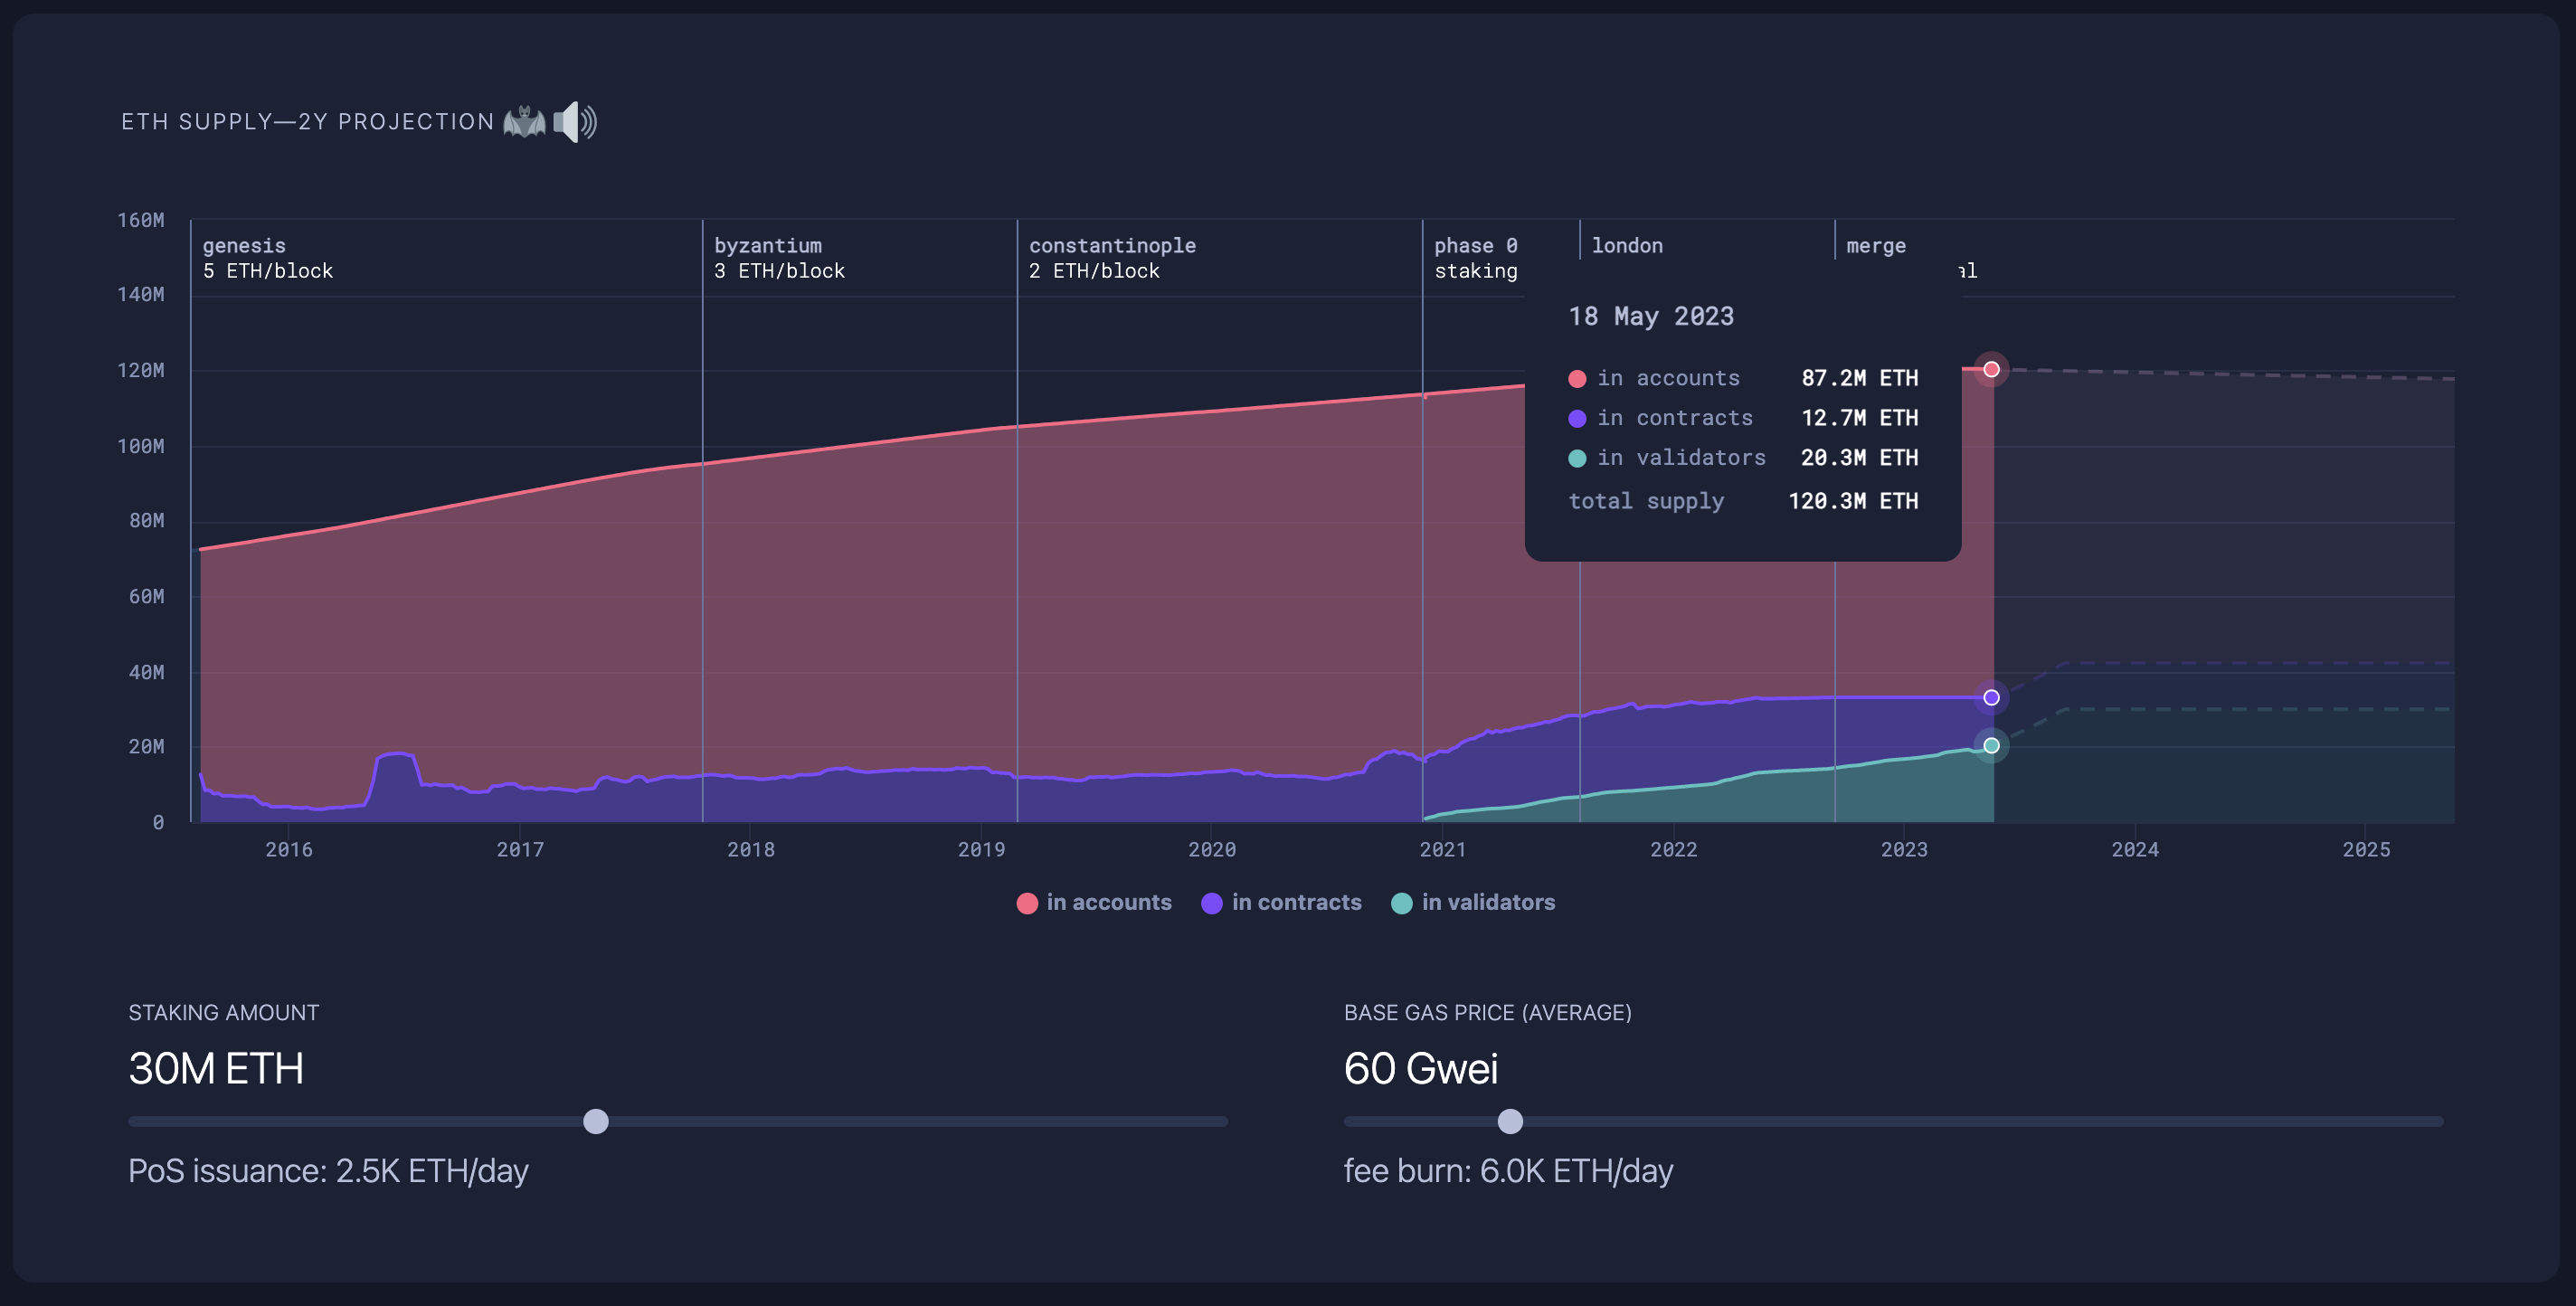
\includegraphics[width=0.9\linewidth]{images/2yprojection}
\caption{2YETH supply projection, 22 May 2023}
\label{fig:2yprojection}
\end{center}
\end{figure}

\begin{figure}[htbp]
\begin{center}
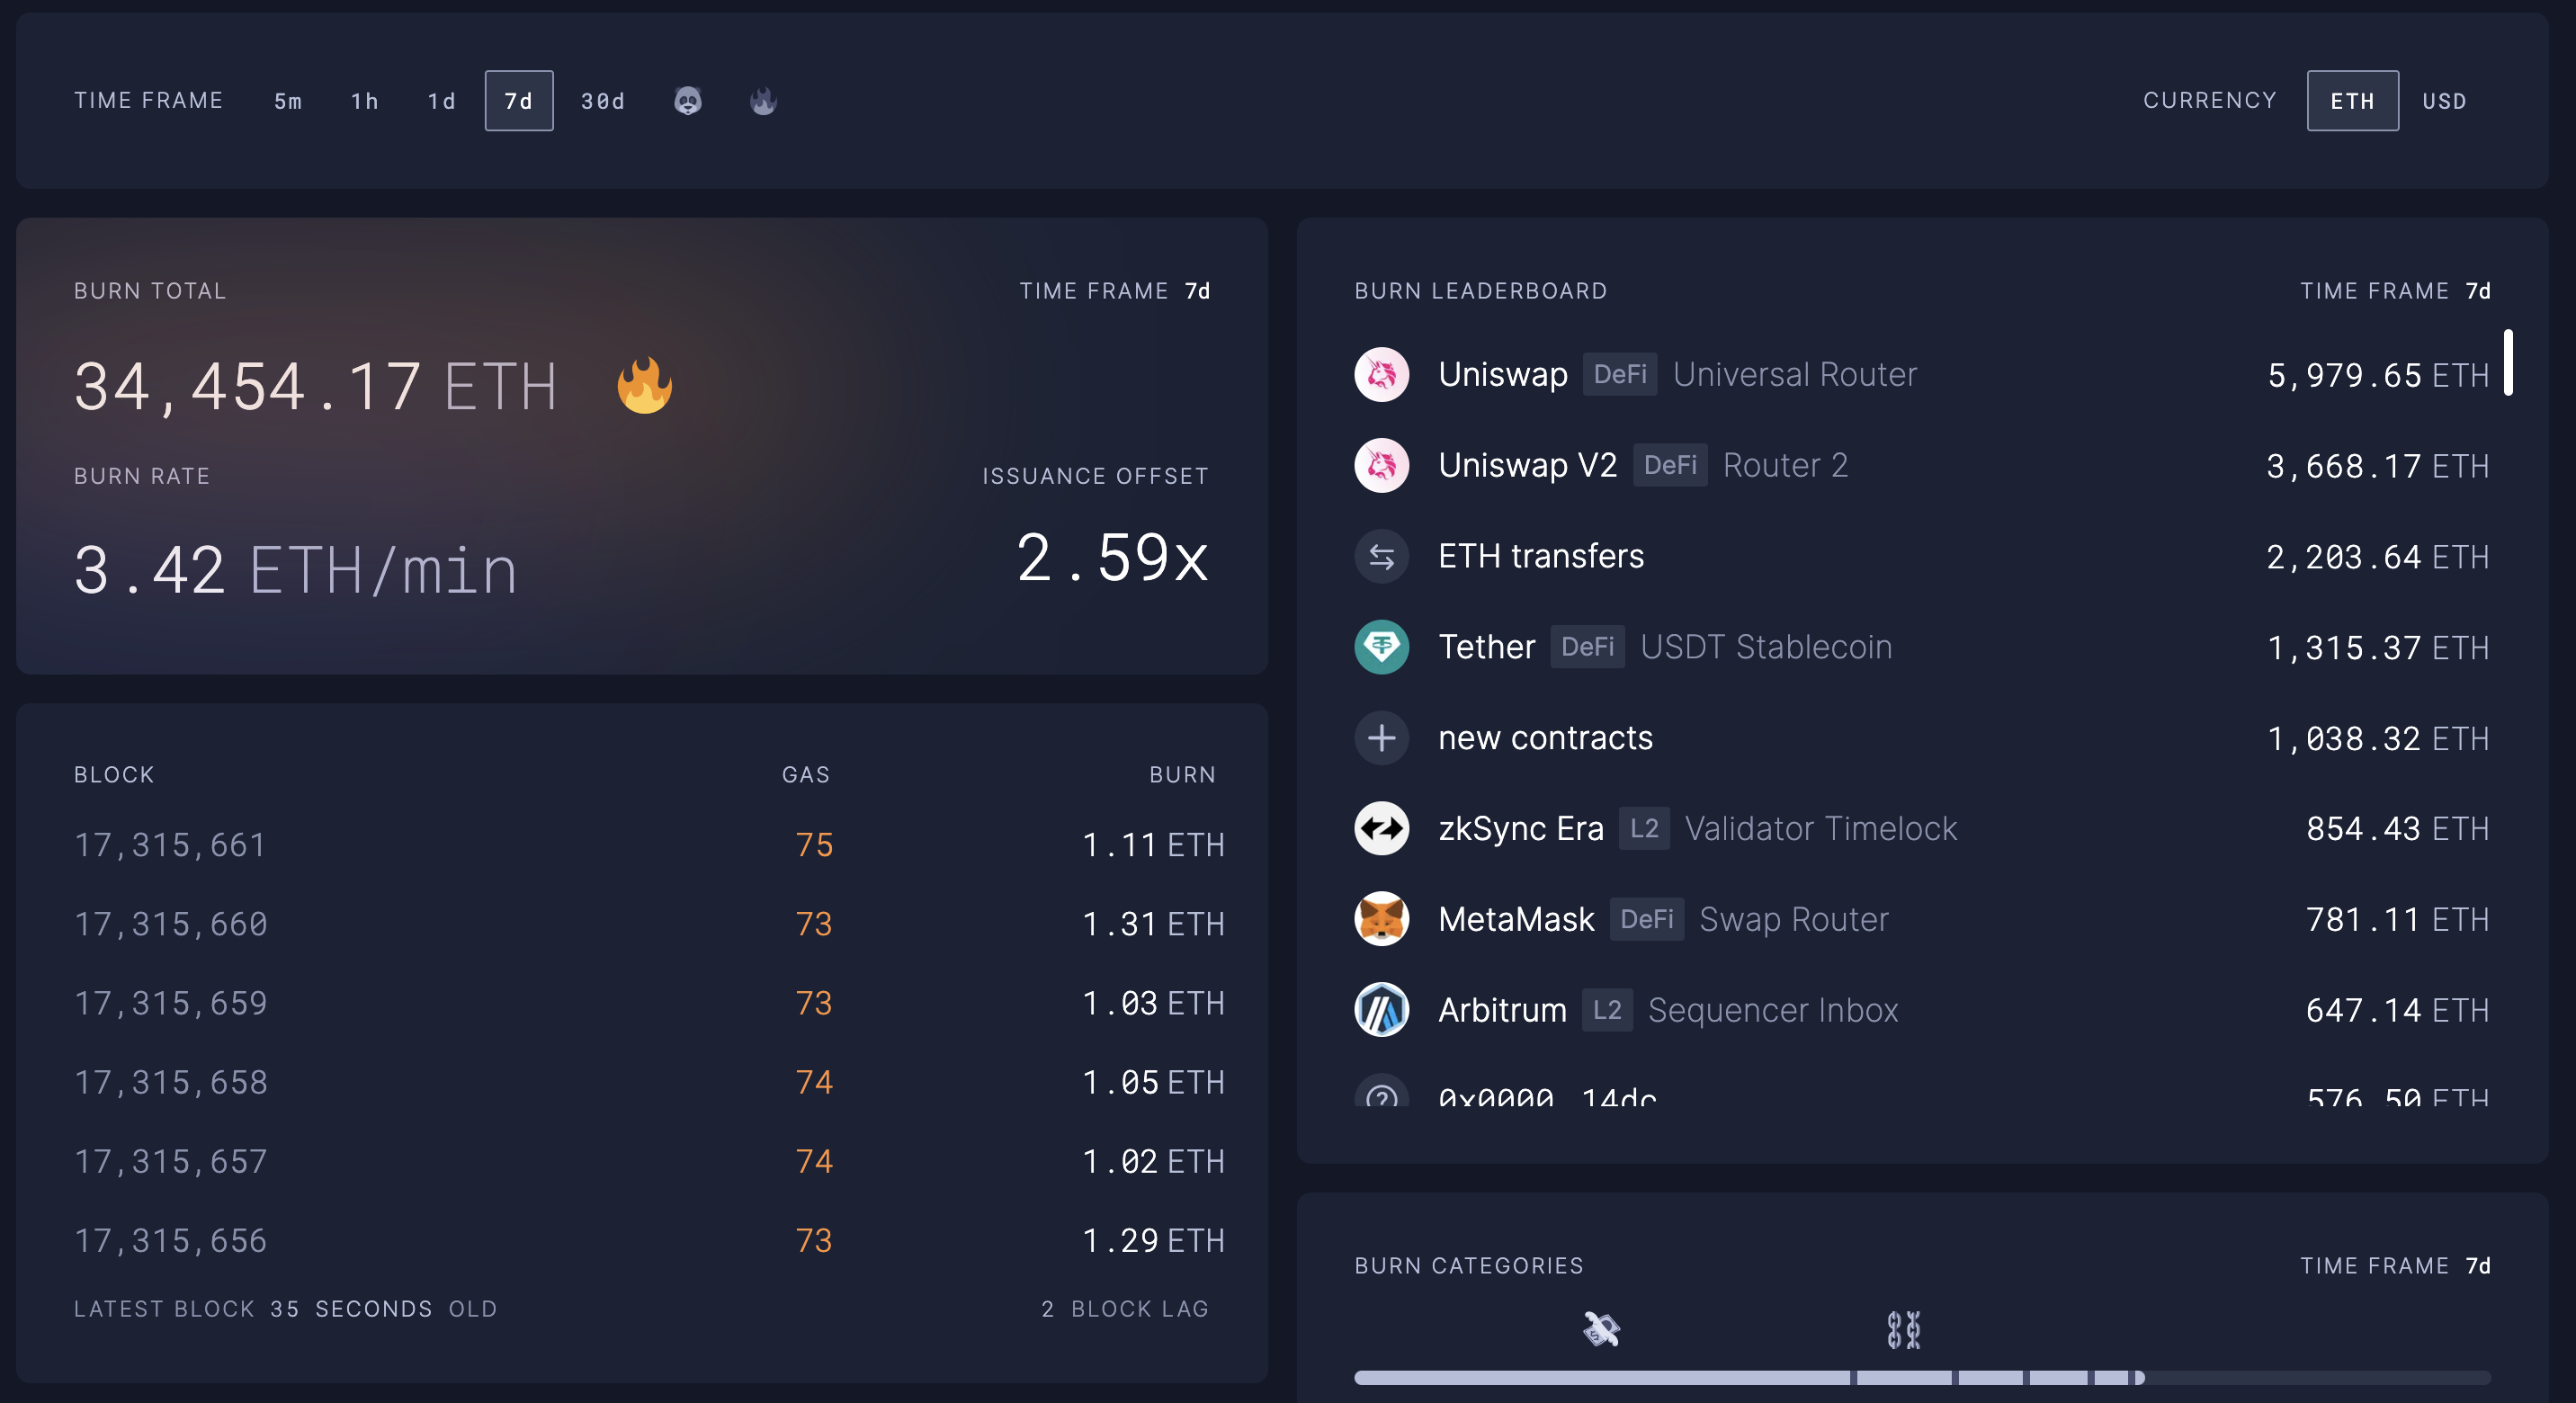
\includegraphics[width=0.9\linewidth]{images/totalburn}
\caption{Total burn and rate for selected time interval; latest block gas and burn leaderboard, 22 May 2023}
\label{fig:totalburn}
\end{center}
\end{figure}

\begin{figure}[htbp]
\begin{center}
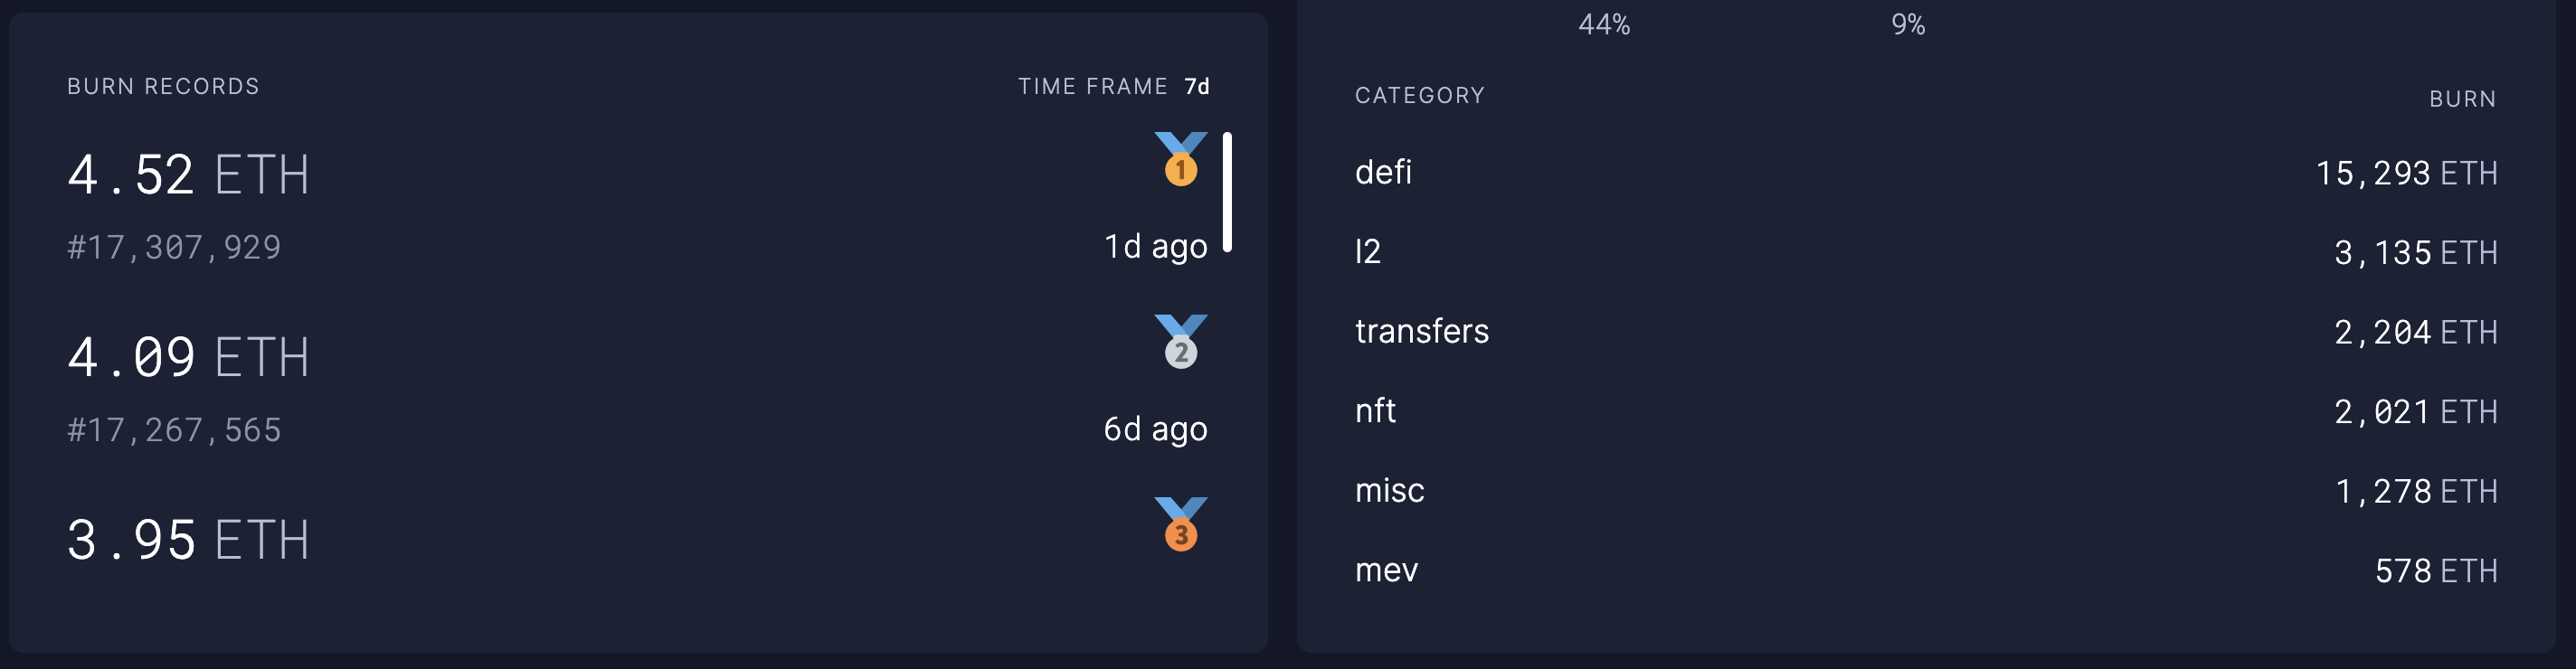
\includegraphics[width=0.9\linewidth]{images/records}
\caption{Burn records (top 3) and top 5 categories for most ETH burnt, 22 May 2023}
\label{fig:records}
\end{center}
\end{figure}

\begin{figure}[htbp]
\begin{center}
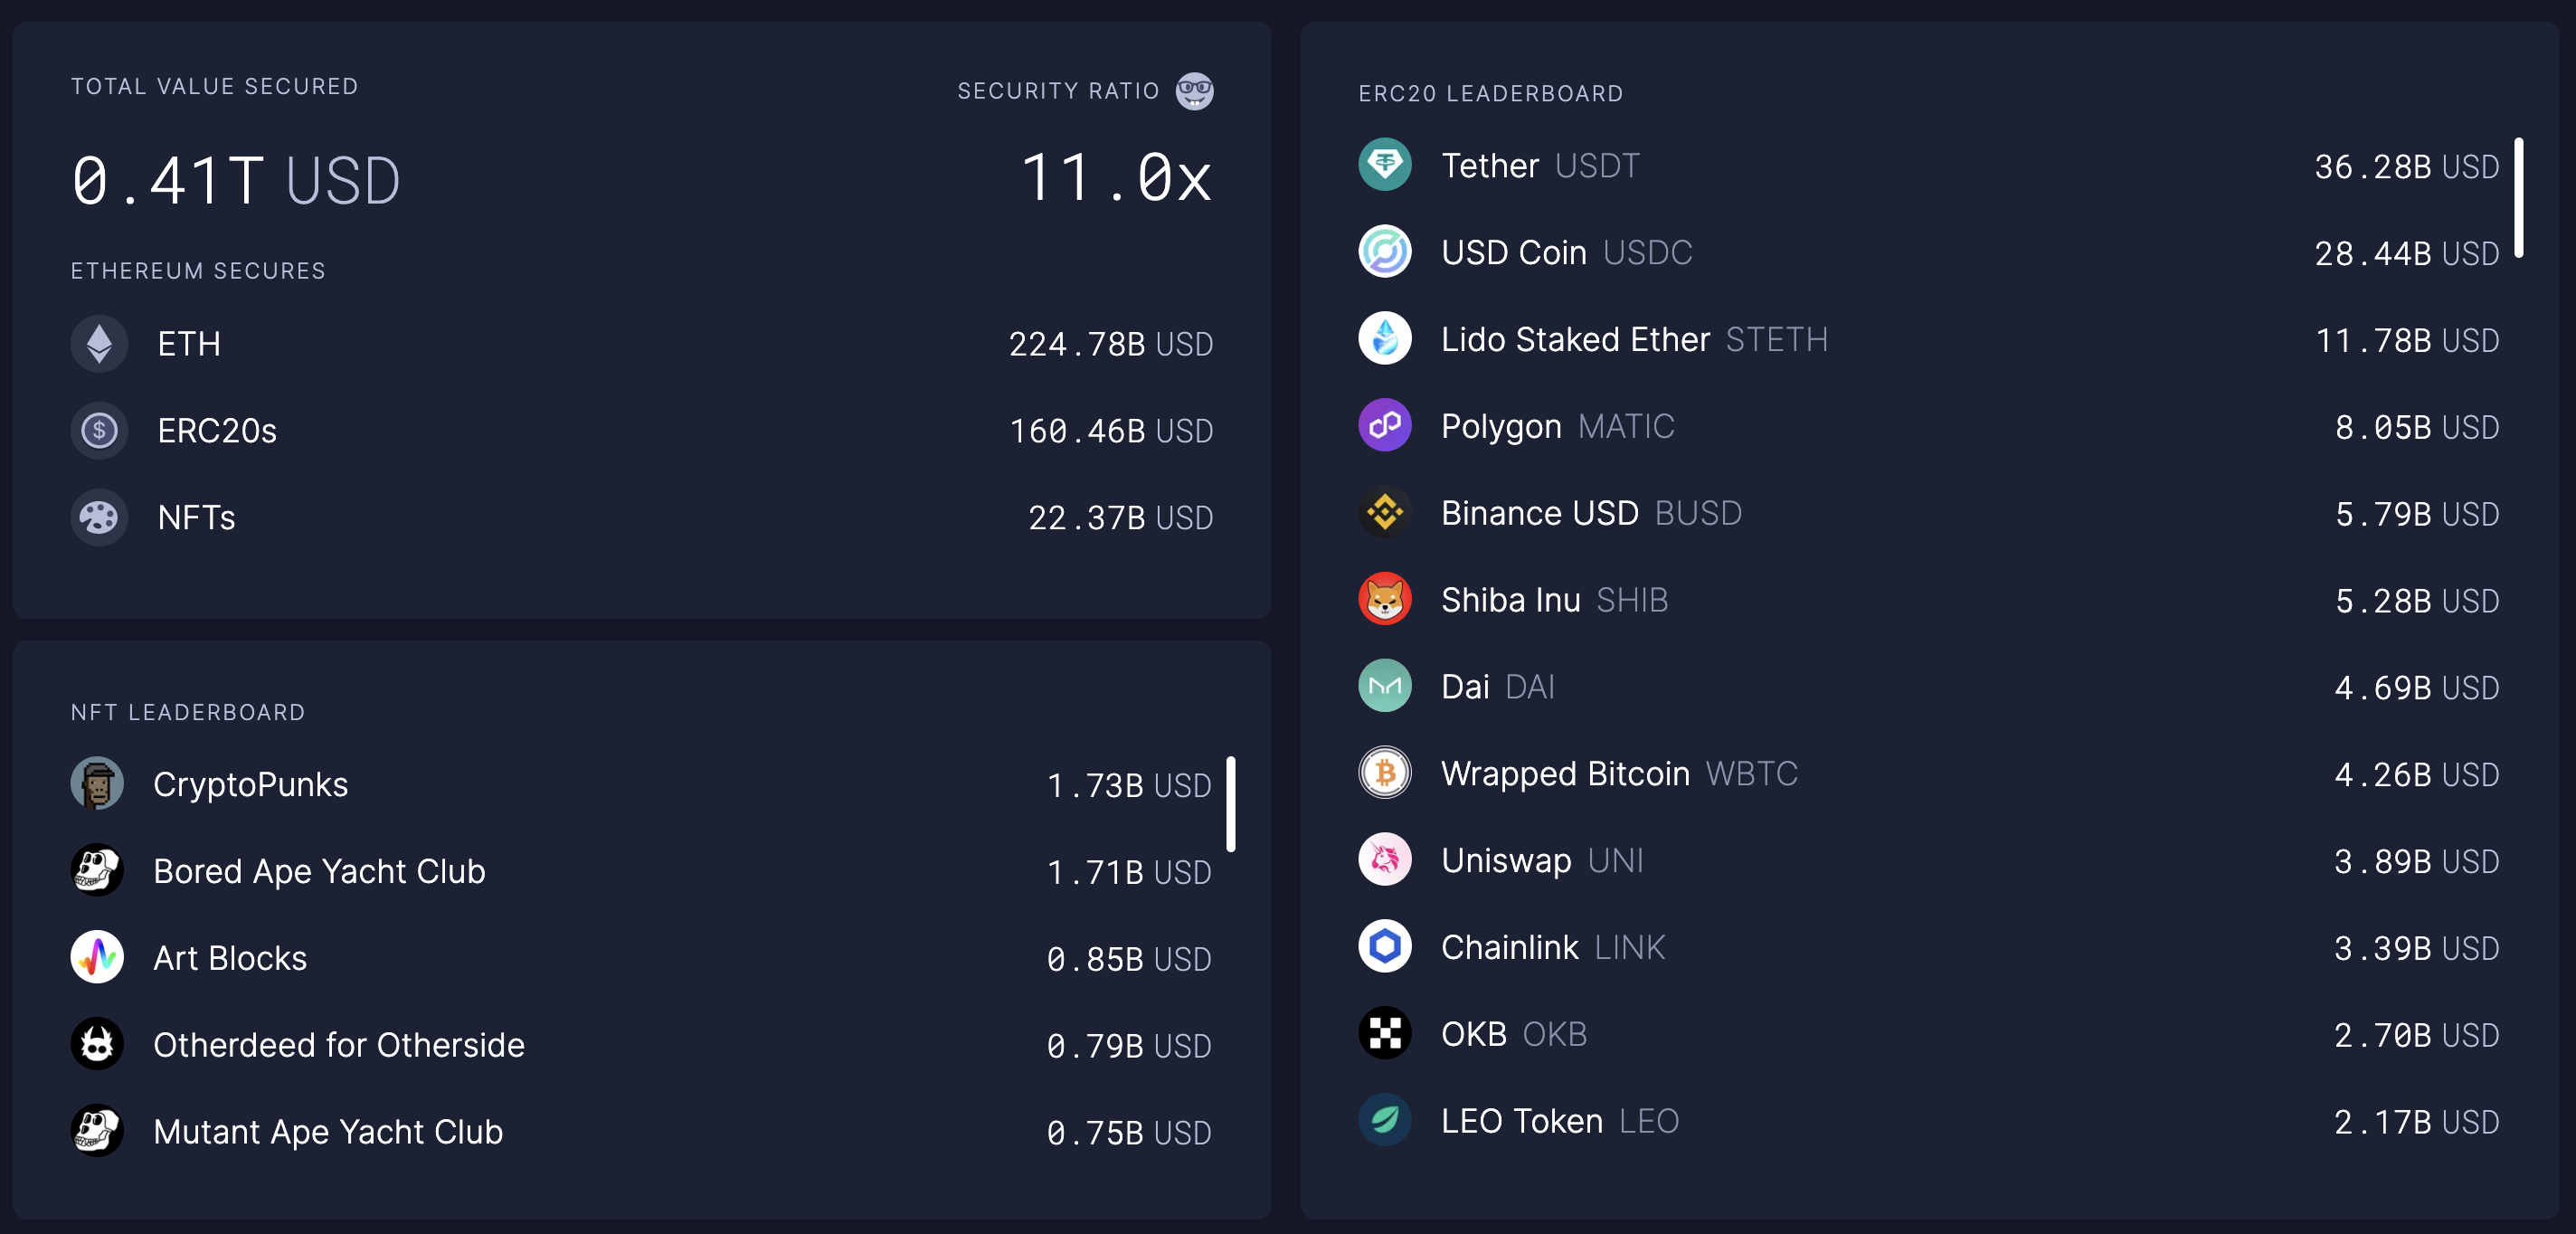
\includegraphics[width=0.9\linewidth]{images/tvs}
\caption{Statistics for total value secured (TVS), including NFT and ERC20 leaderboards, 22 May 2023}
\label{fig:tvs}
\end{center}
\end{figure}

\begin{figure}[htbp]
\begin{center}
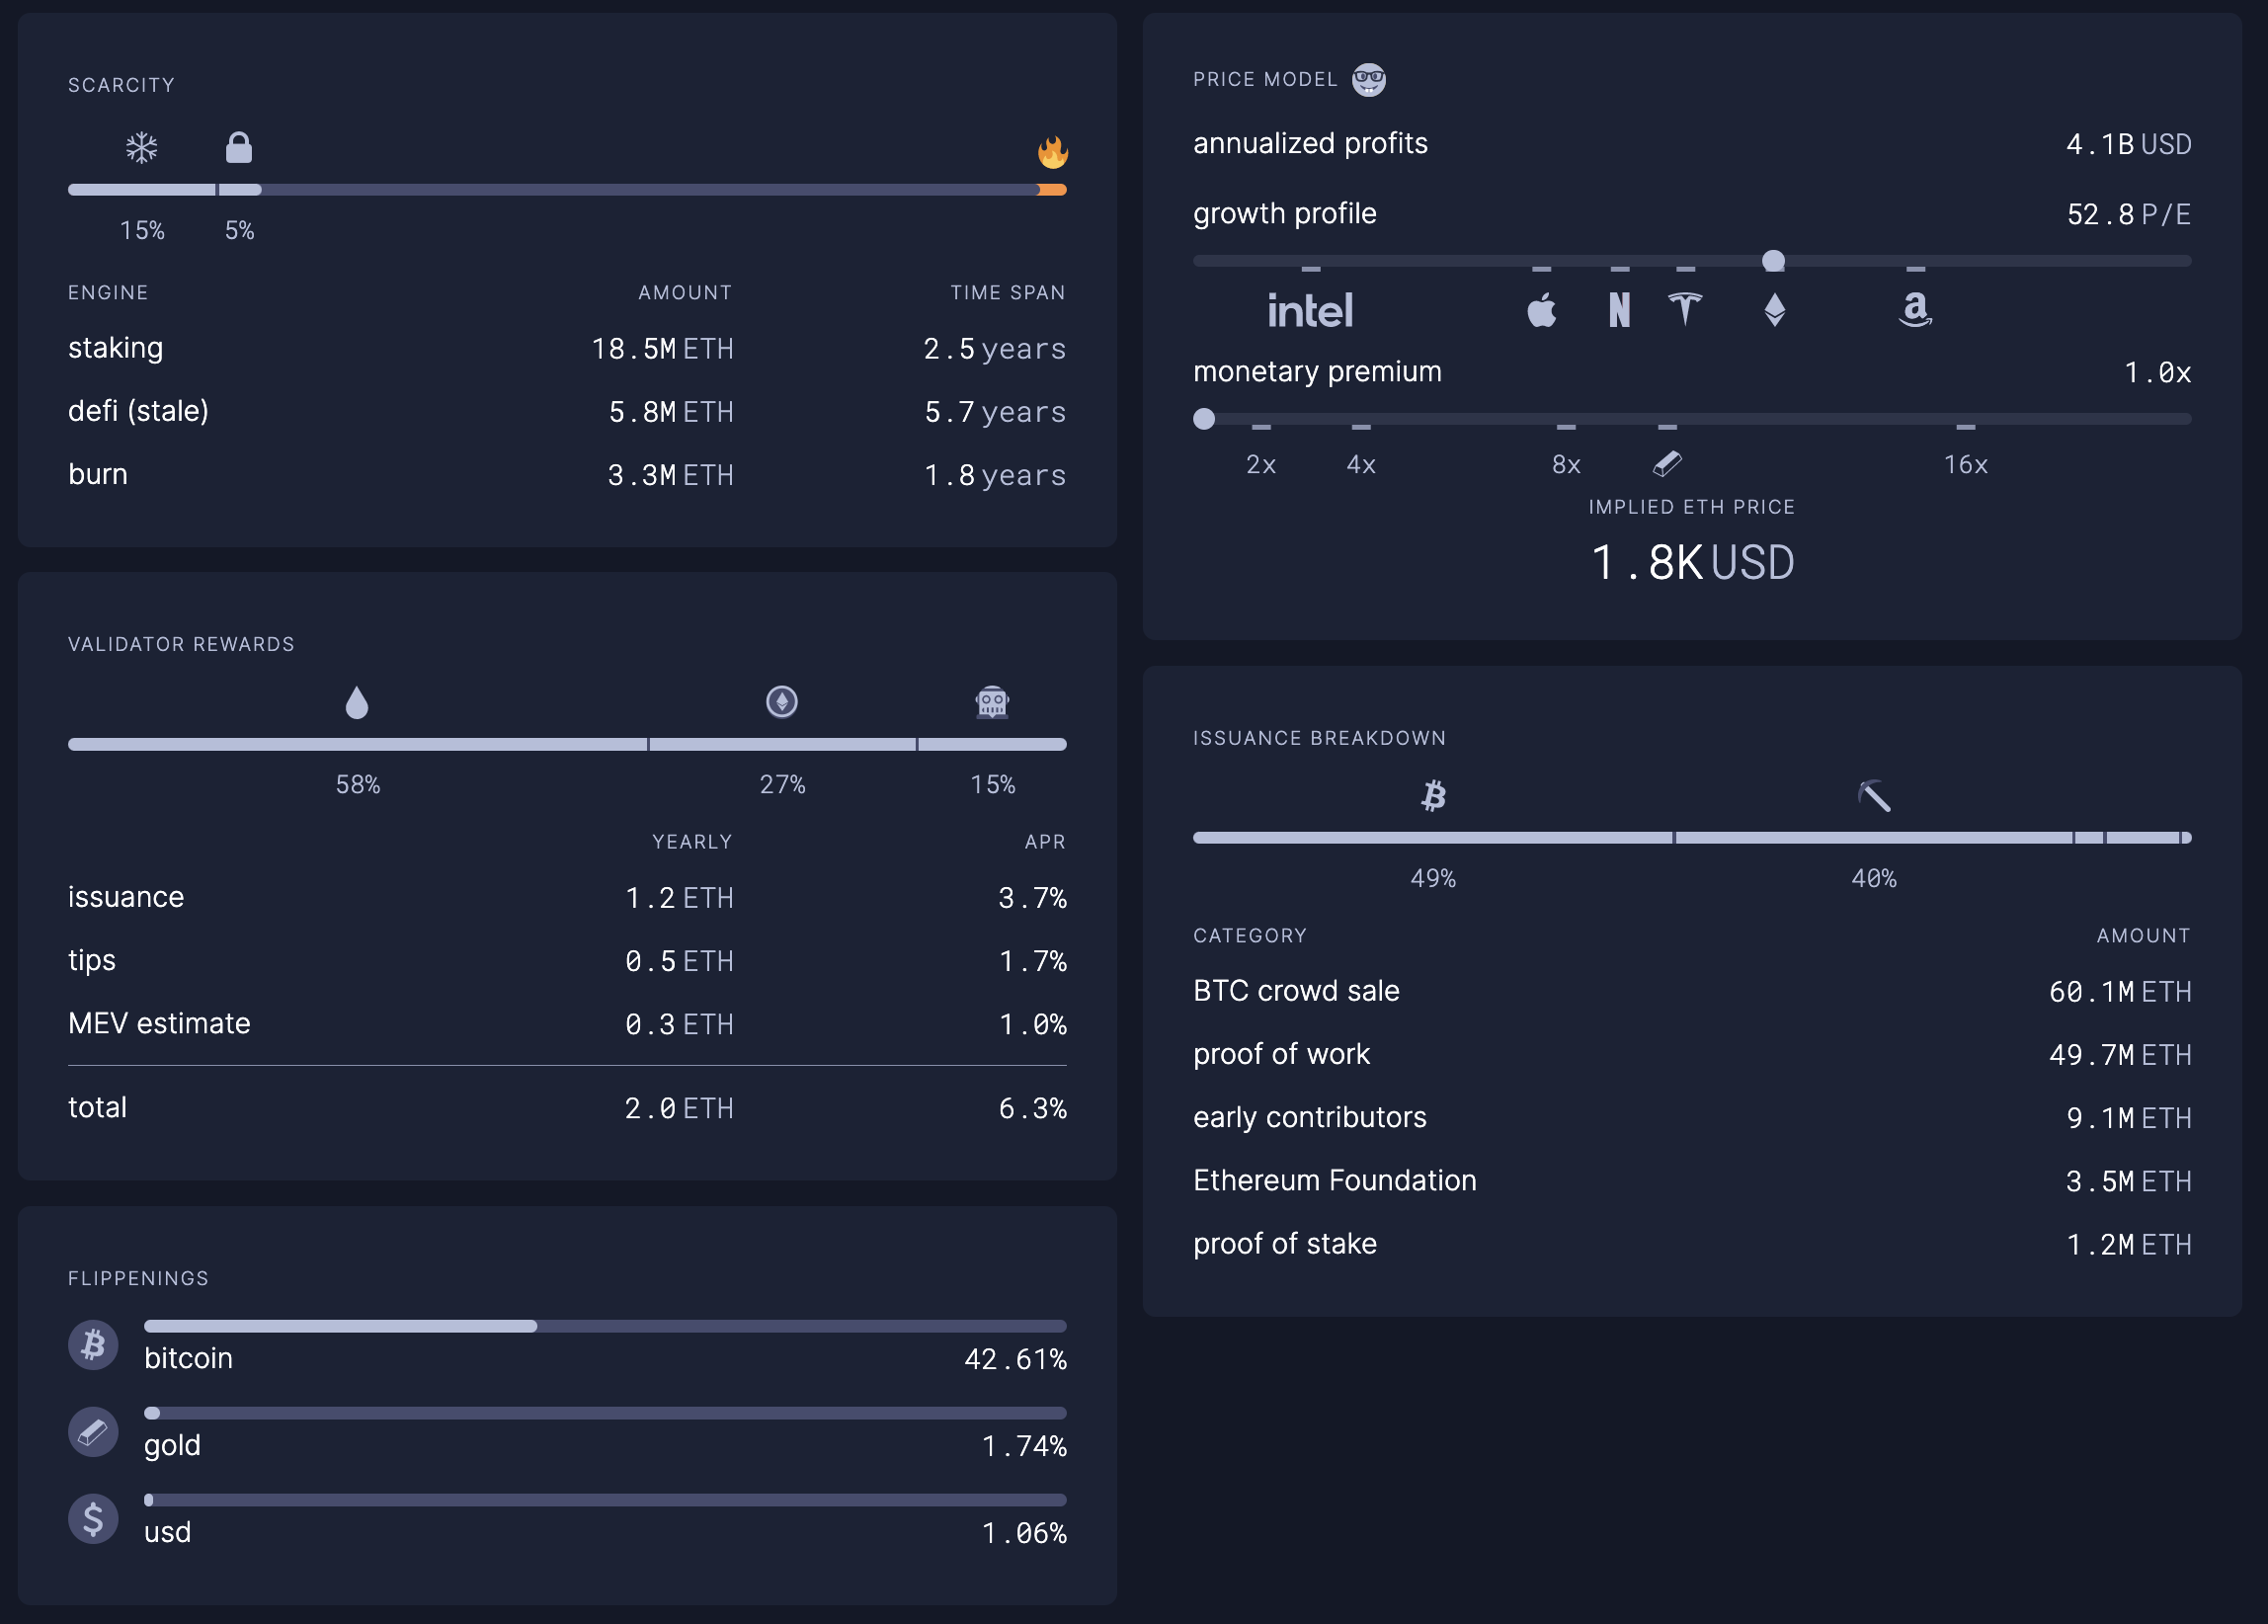
\includegraphics[width=0.9\linewidth]{images/monetary}
\caption{Monetary premium shows Scarcity (staking, defi, burn), Validator rewards (issuance, tips, mev, Flippenings (bitcoin, gold and usd), Issuance breakdown by category and an interactive price model based on selected growth profile and monetary premium, 22 May 2023}
\label{fig:monetary}
\end{center}
\end{figure}

\clearpage
% --------------------------------------
\subsubsection*{Etherscan}
% --------------------------------------
There are several webpages with detailed information on transactions, blocks, accounts and tokens. In the screenshots below, figures~\ref{fig:txns}-~\ref{fig:erc20} on pages~\pageref{fig:txns}-~\pageref{fig:erc20}), are a few extracts from the detailed information on Etherscan and the data visualisations provided by them. Many of the dashboards allow the user to interact with the data being displayed by entering specific validators, blocks etc, that are of interest, or selecting one of the different time periods available. 

Moreover, there are several summary graphs and visualisations that have been created and are displayed in the \textit{Charts \& Statistics} section of the website. These visualisations are shown in figures~\ref{fig:ethdaily}-~\ref{fig:ethgrowth} on pages~\pageref{fig:ethdaily}~-~\pageref{fig:ethgrowth}. There is some degree of interactivity in these charts and diagrams, which includes the ability to zoom in on a section of a graph in several instances.\\

\begin{figure}[htbp]
\begin{center}
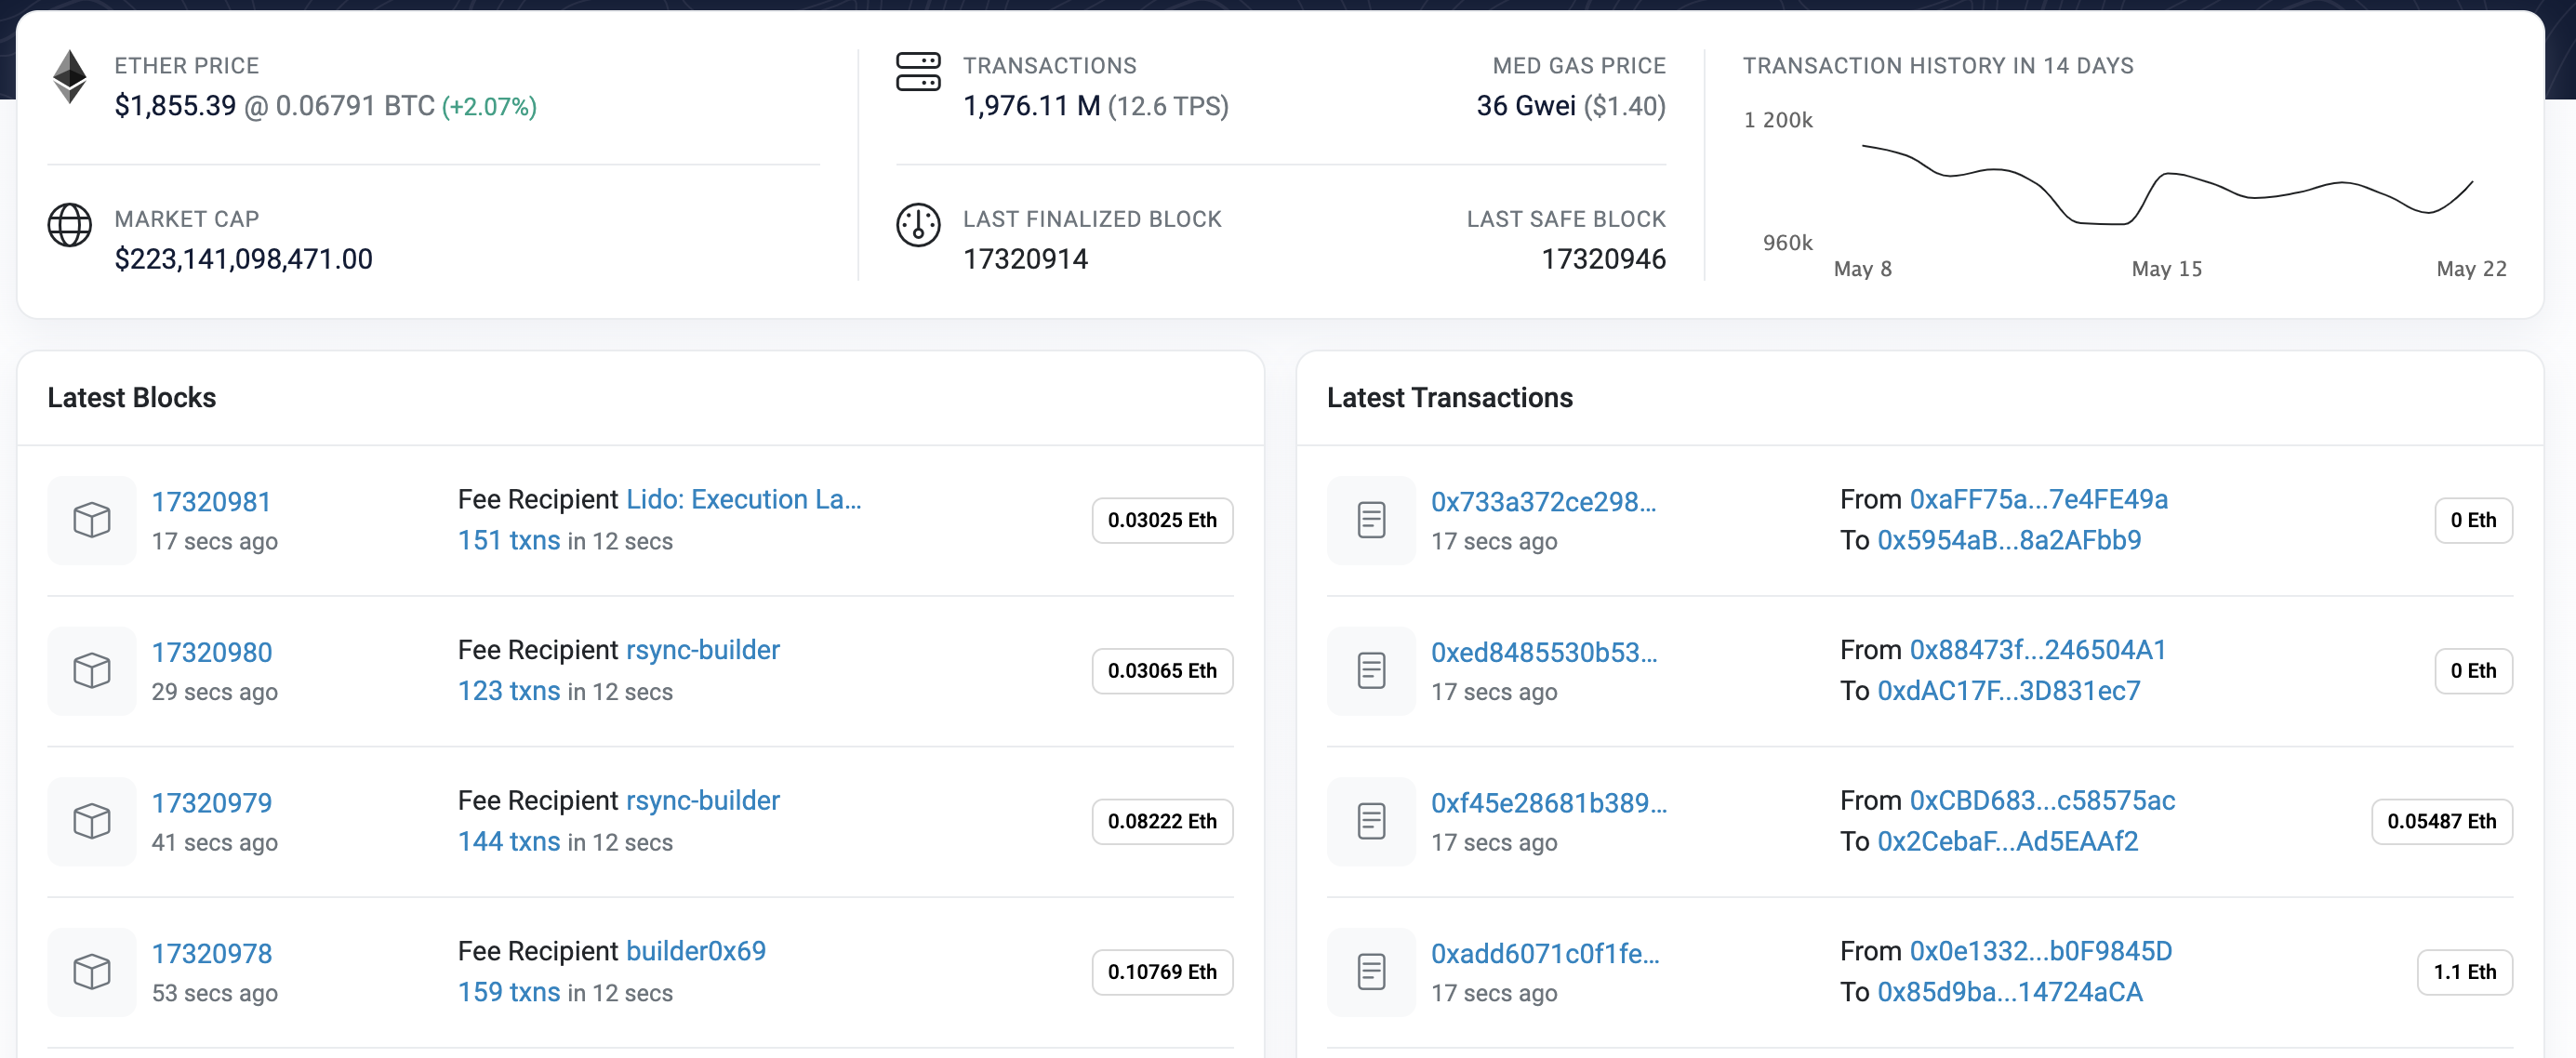
\includegraphics[width=\linewidth]{images/etherscan}
\caption{Etherscan home page, 23 May 2023}
\label{fig:ethscan}
\end{center}
\end{figure}
\clearpage
\textbf{Detailed blockchain data}\\
% ------------------------------------------
\begin{figure}[htbp]
\begin{center}
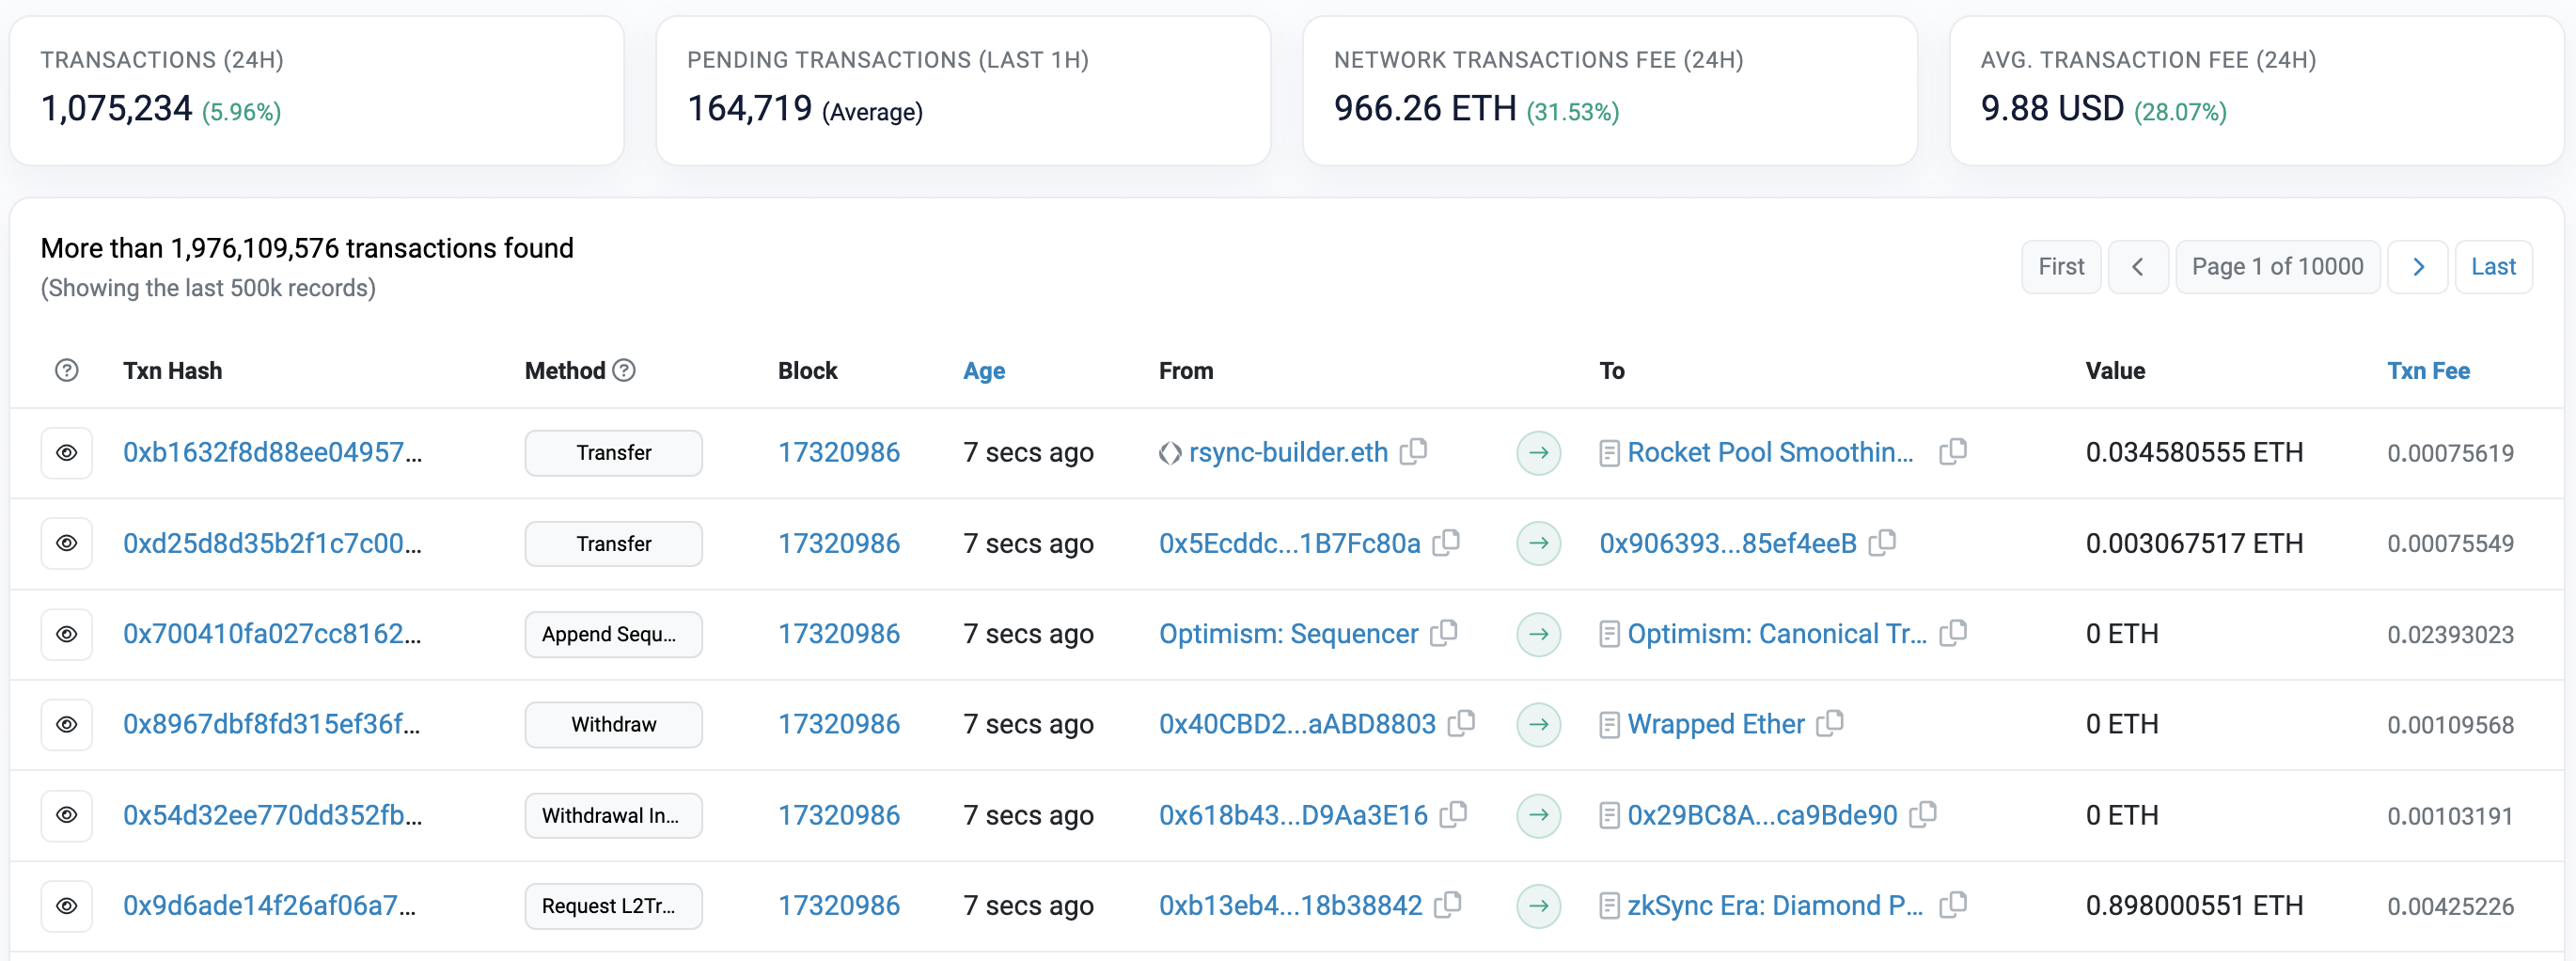
\includegraphics[width=0.48\linewidth]{images/txns}
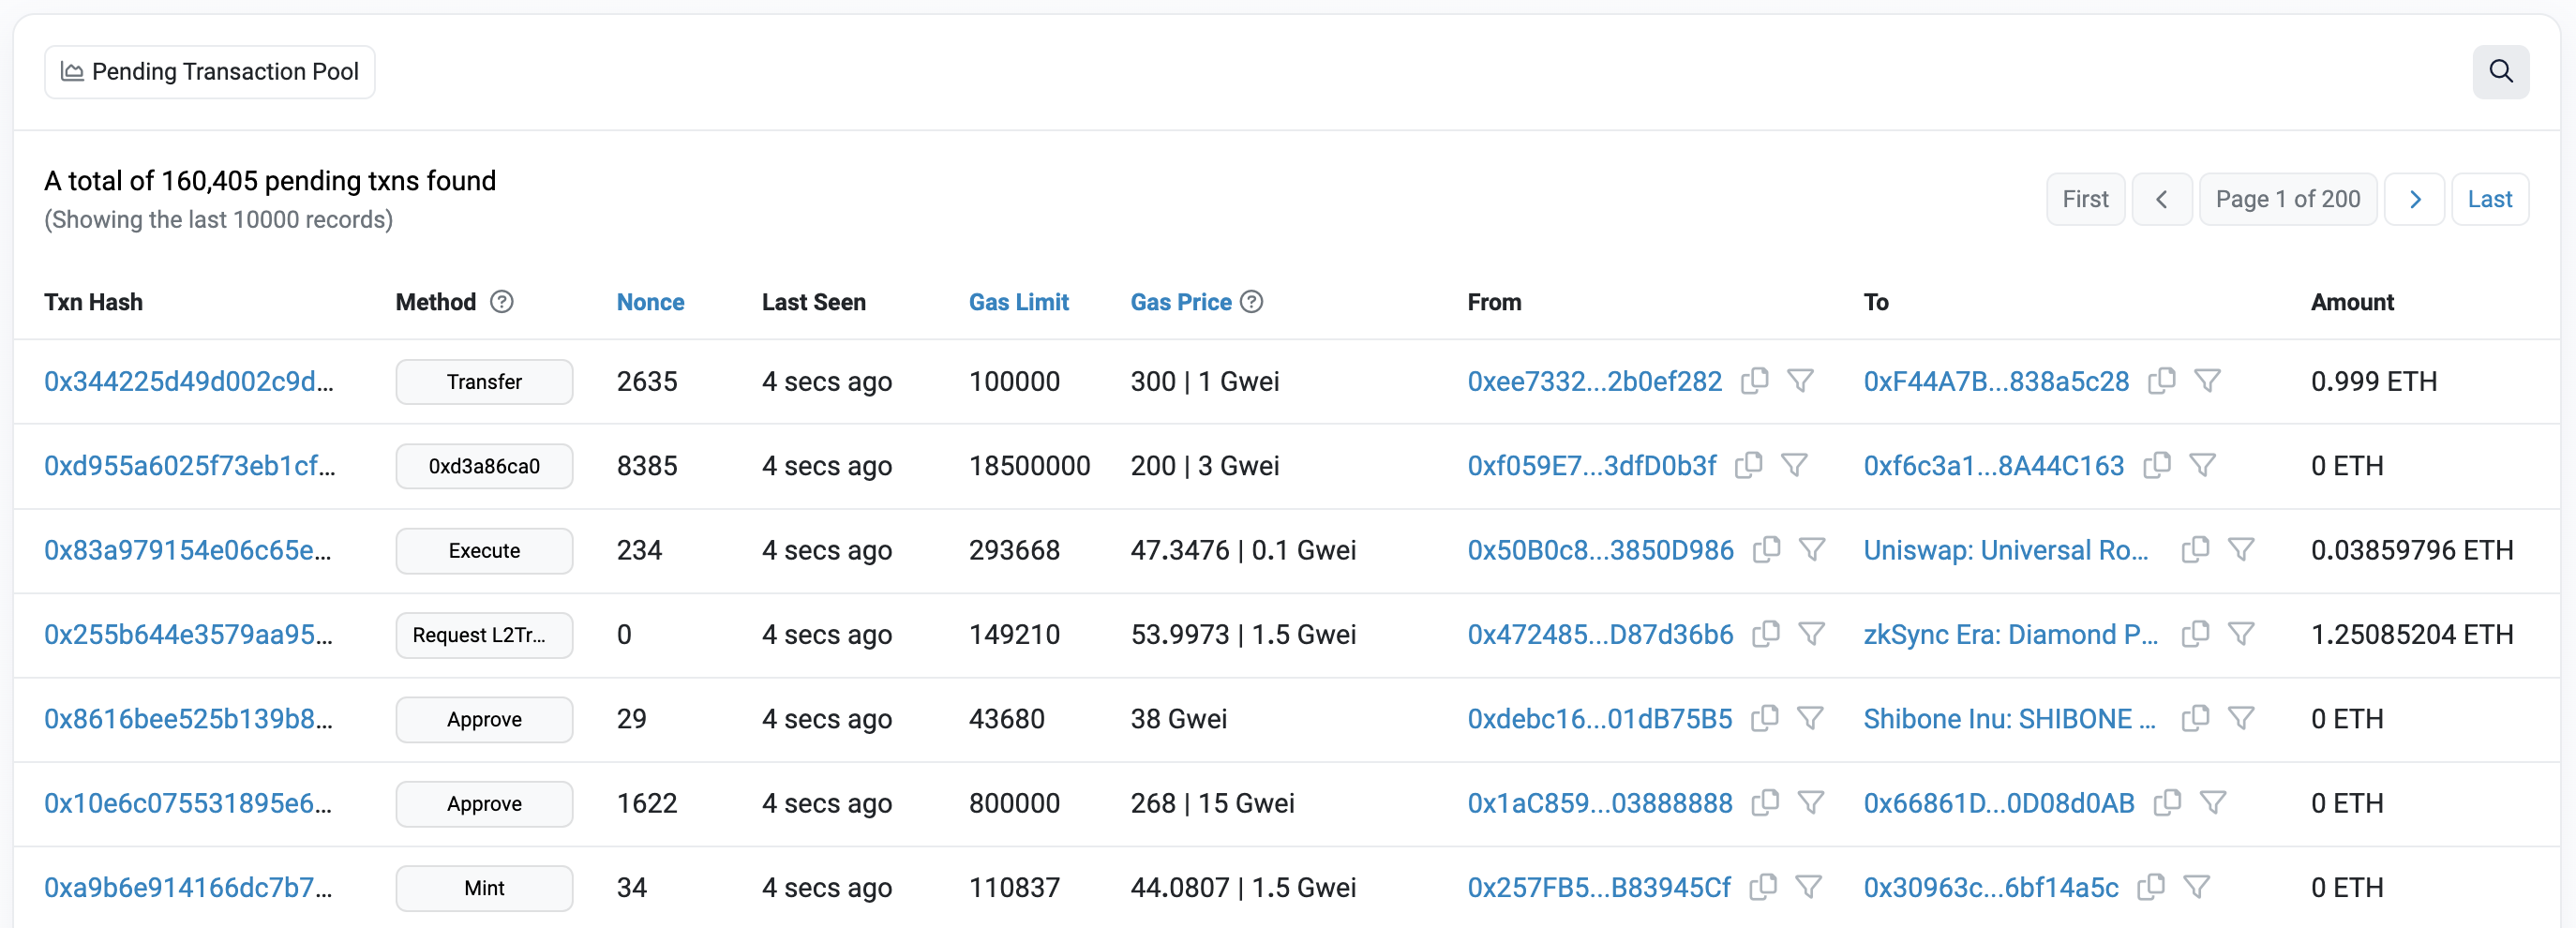
\includegraphics[width=0.48\linewidth]{images/pendtxns} \\
(a)\hspace{160pt}        (b)\\
\caption{Transactions (a) and pending transactions (b) from Etherscan (23 May 2023)}
\label{fig:txns}
\end{center}
\end{figure}


\begin{figure}[htbp]
\begin{center}
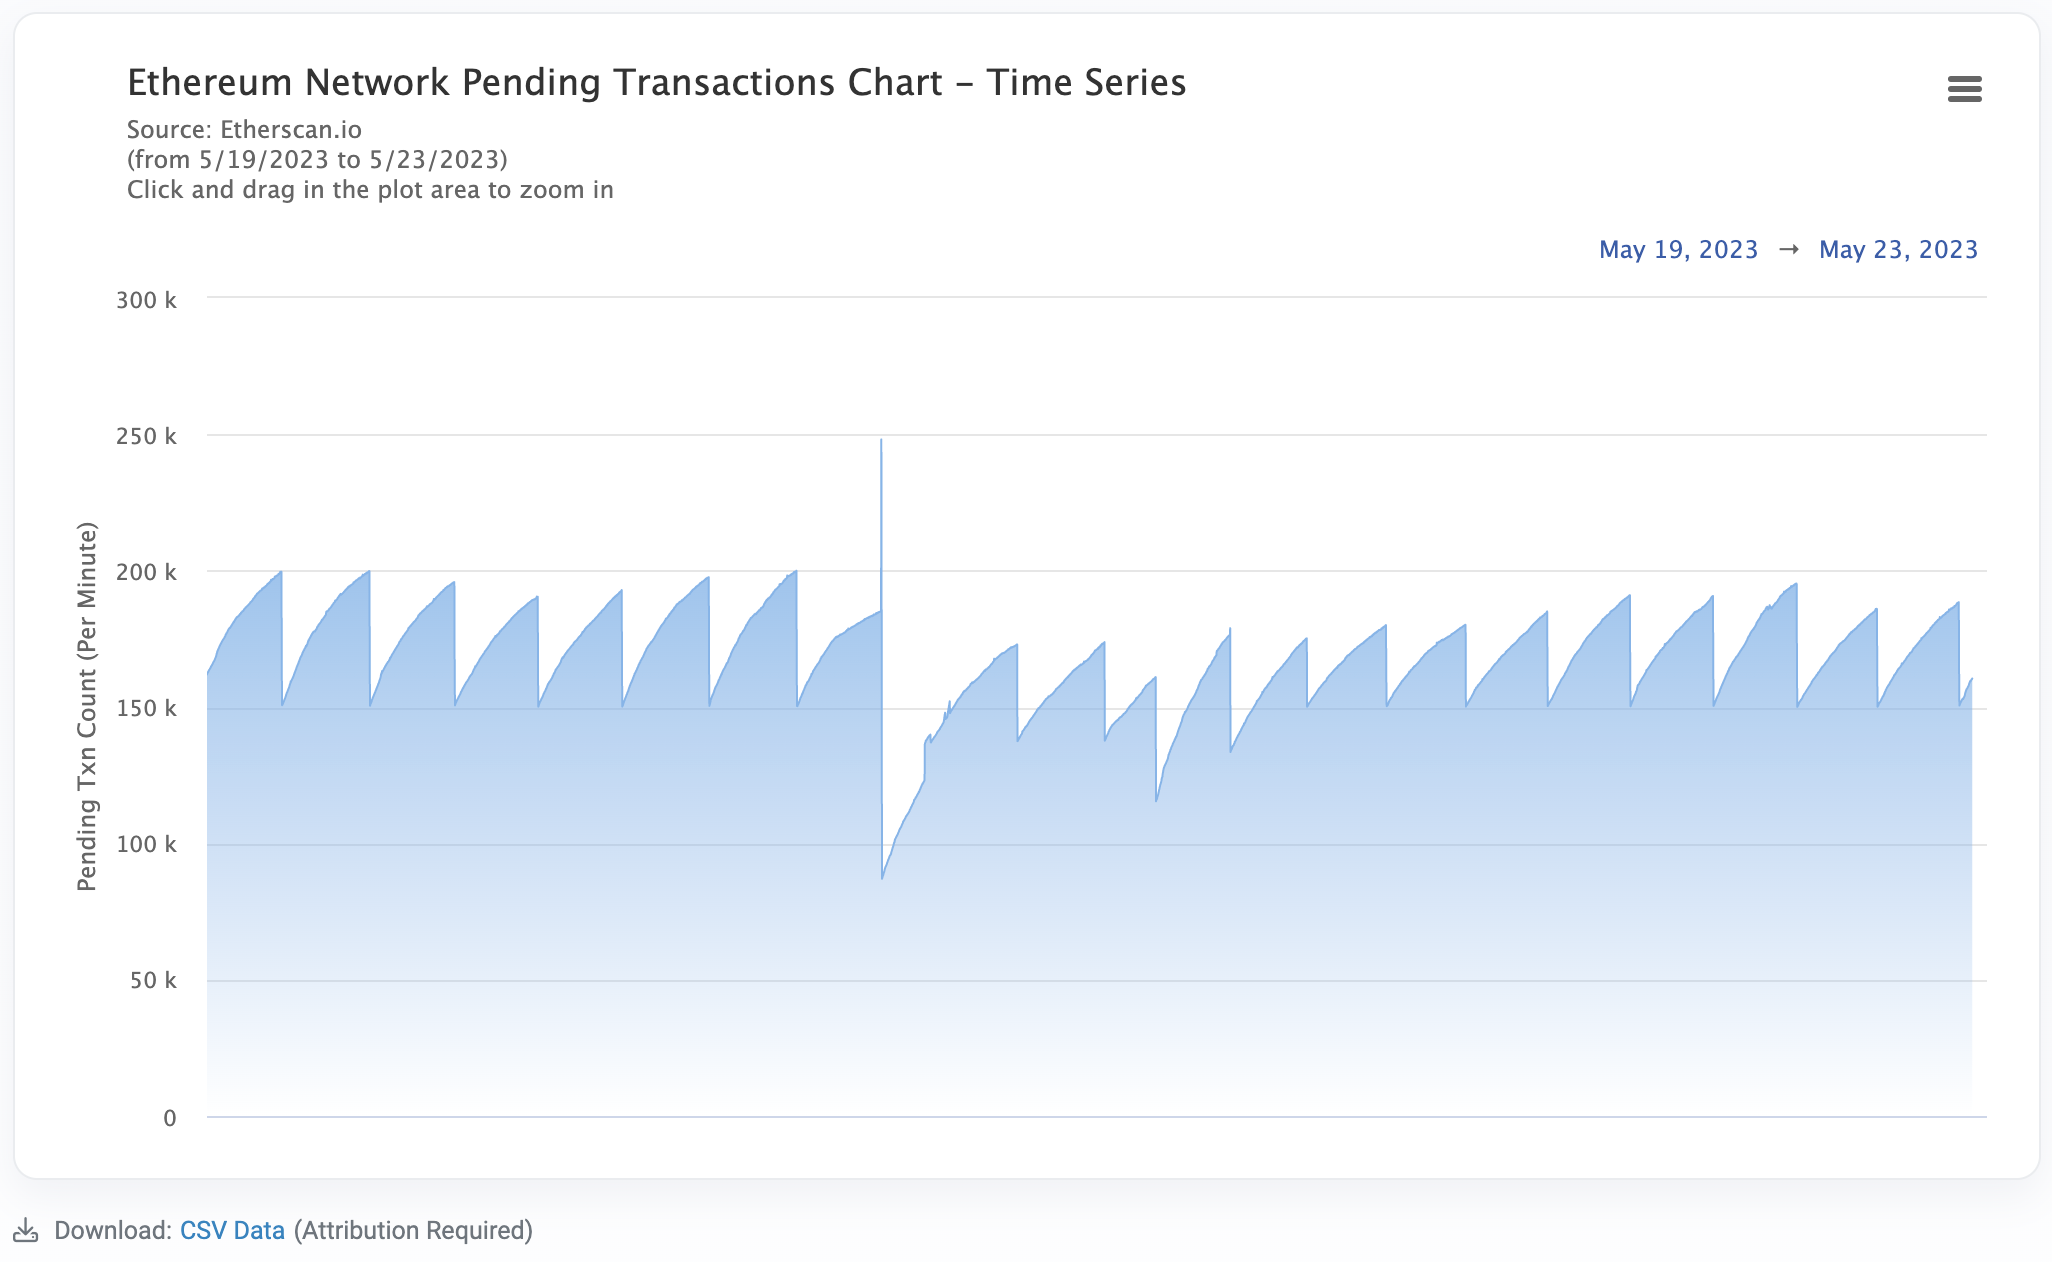
\includegraphics[width=0.48\linewidth]{images/pendchart}
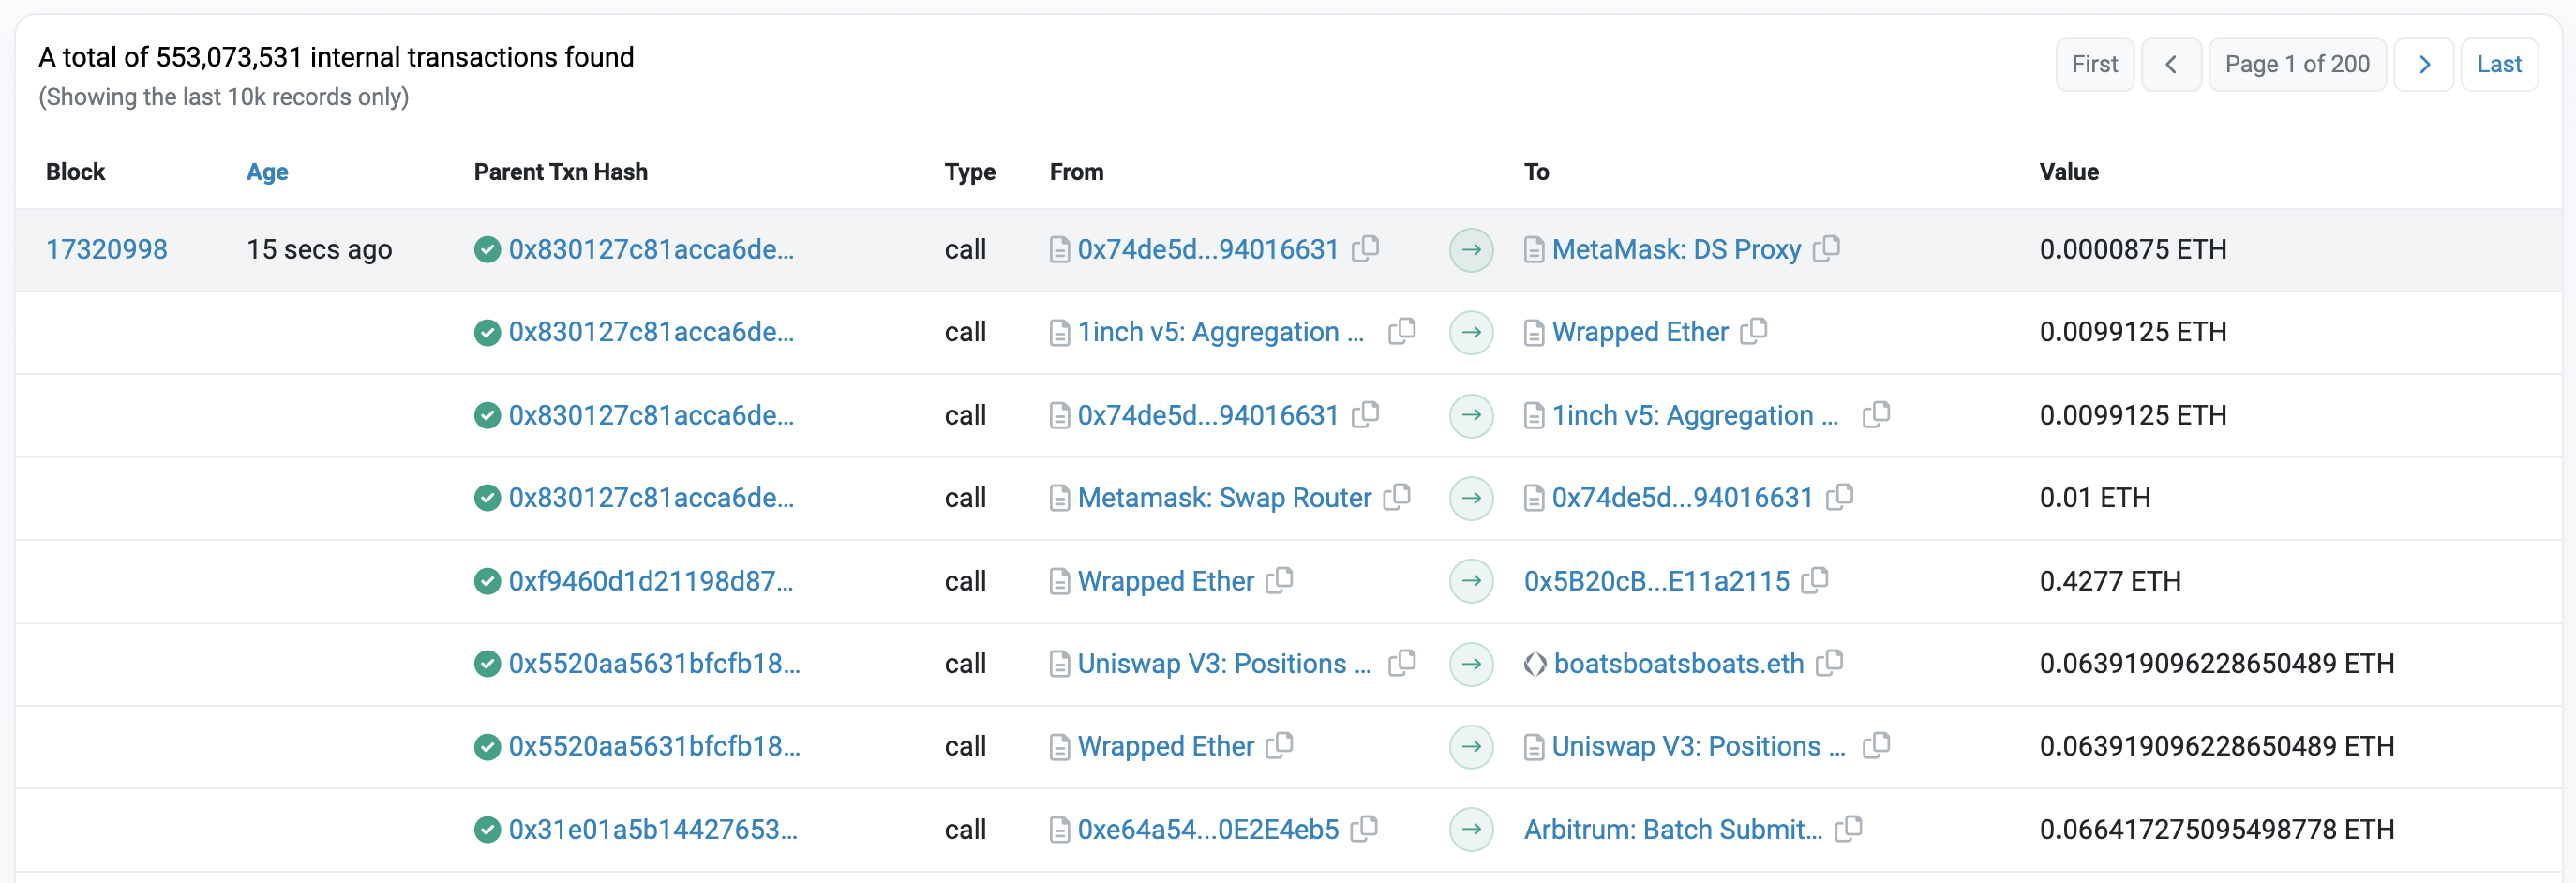
\includegraphics[width=0.48\linewidth]{images/internal} \\
(a)\hspace{160pt}        (b)\\
\caption{Chart of pending transactions (a) and contract internal transactions (b) from Etherscan (23 May 2023)}
\label{fig:pendchart}
\end{center}
\end{figure}

\begin{figure}[htbp]
\begin{center}
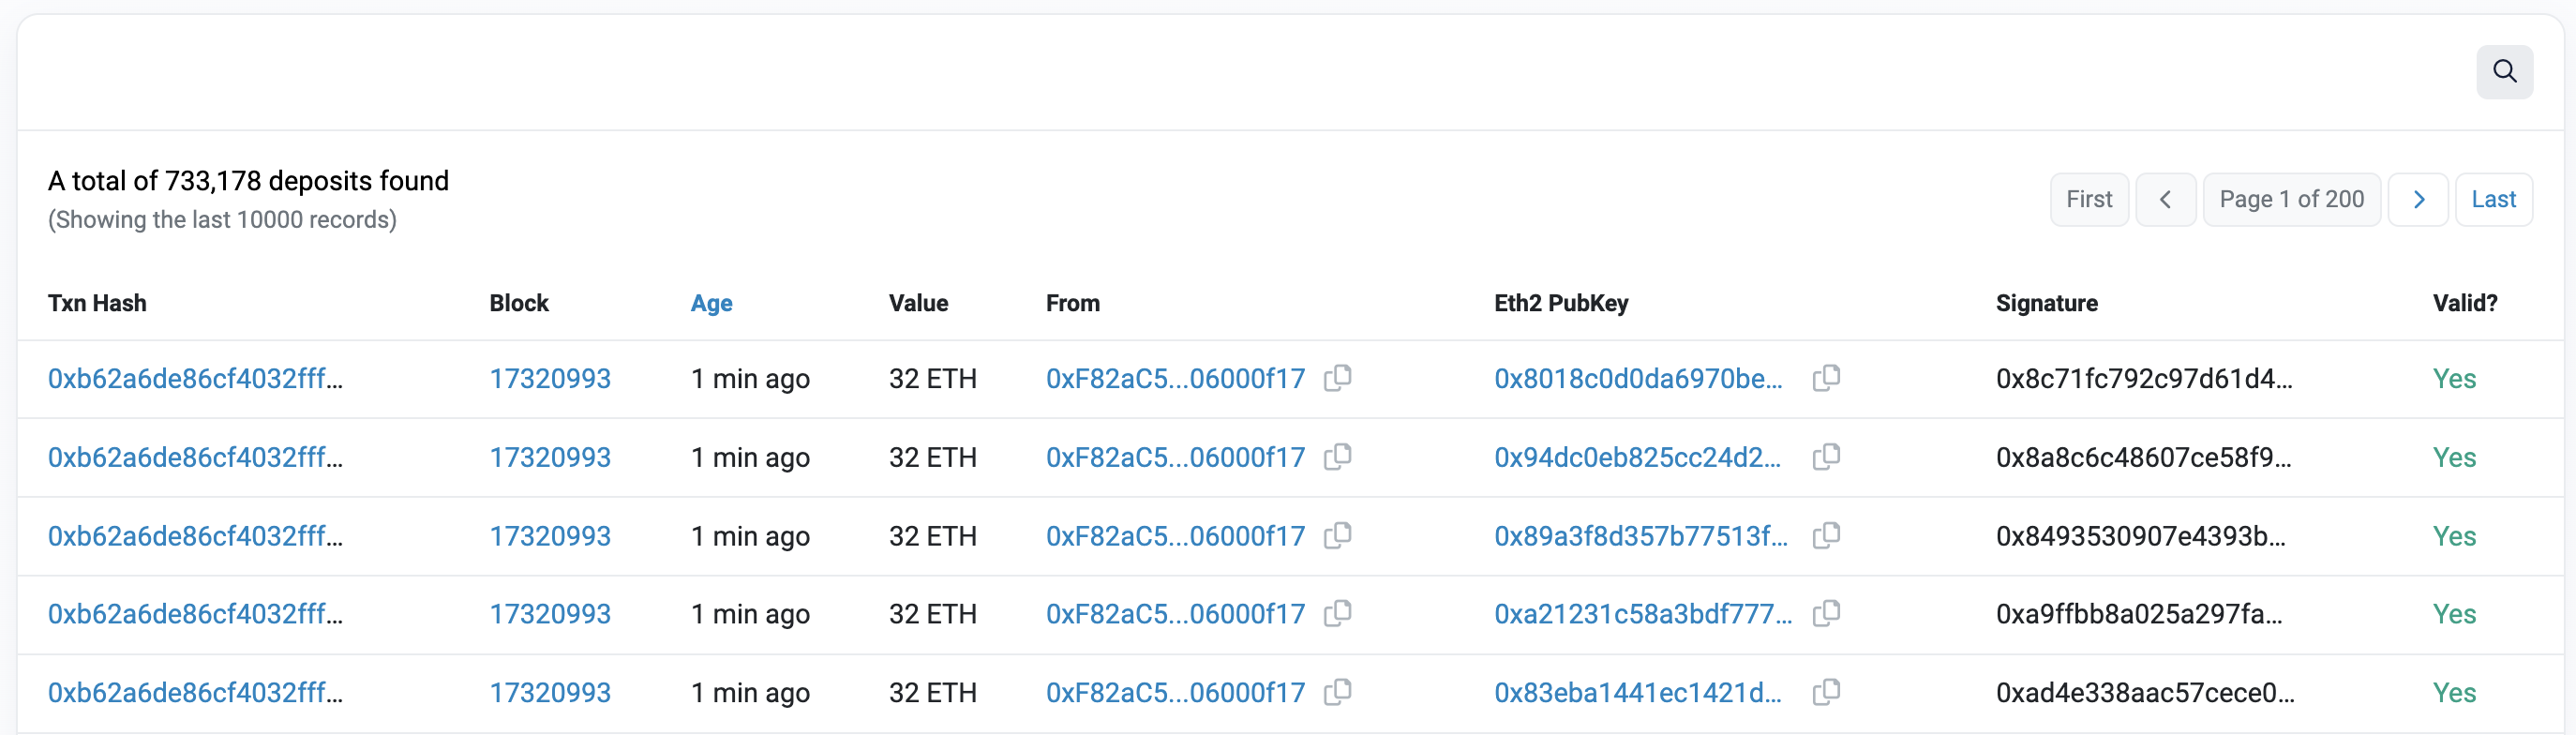
\includegraphics[width=0.48\linewidth]{images/deposits}
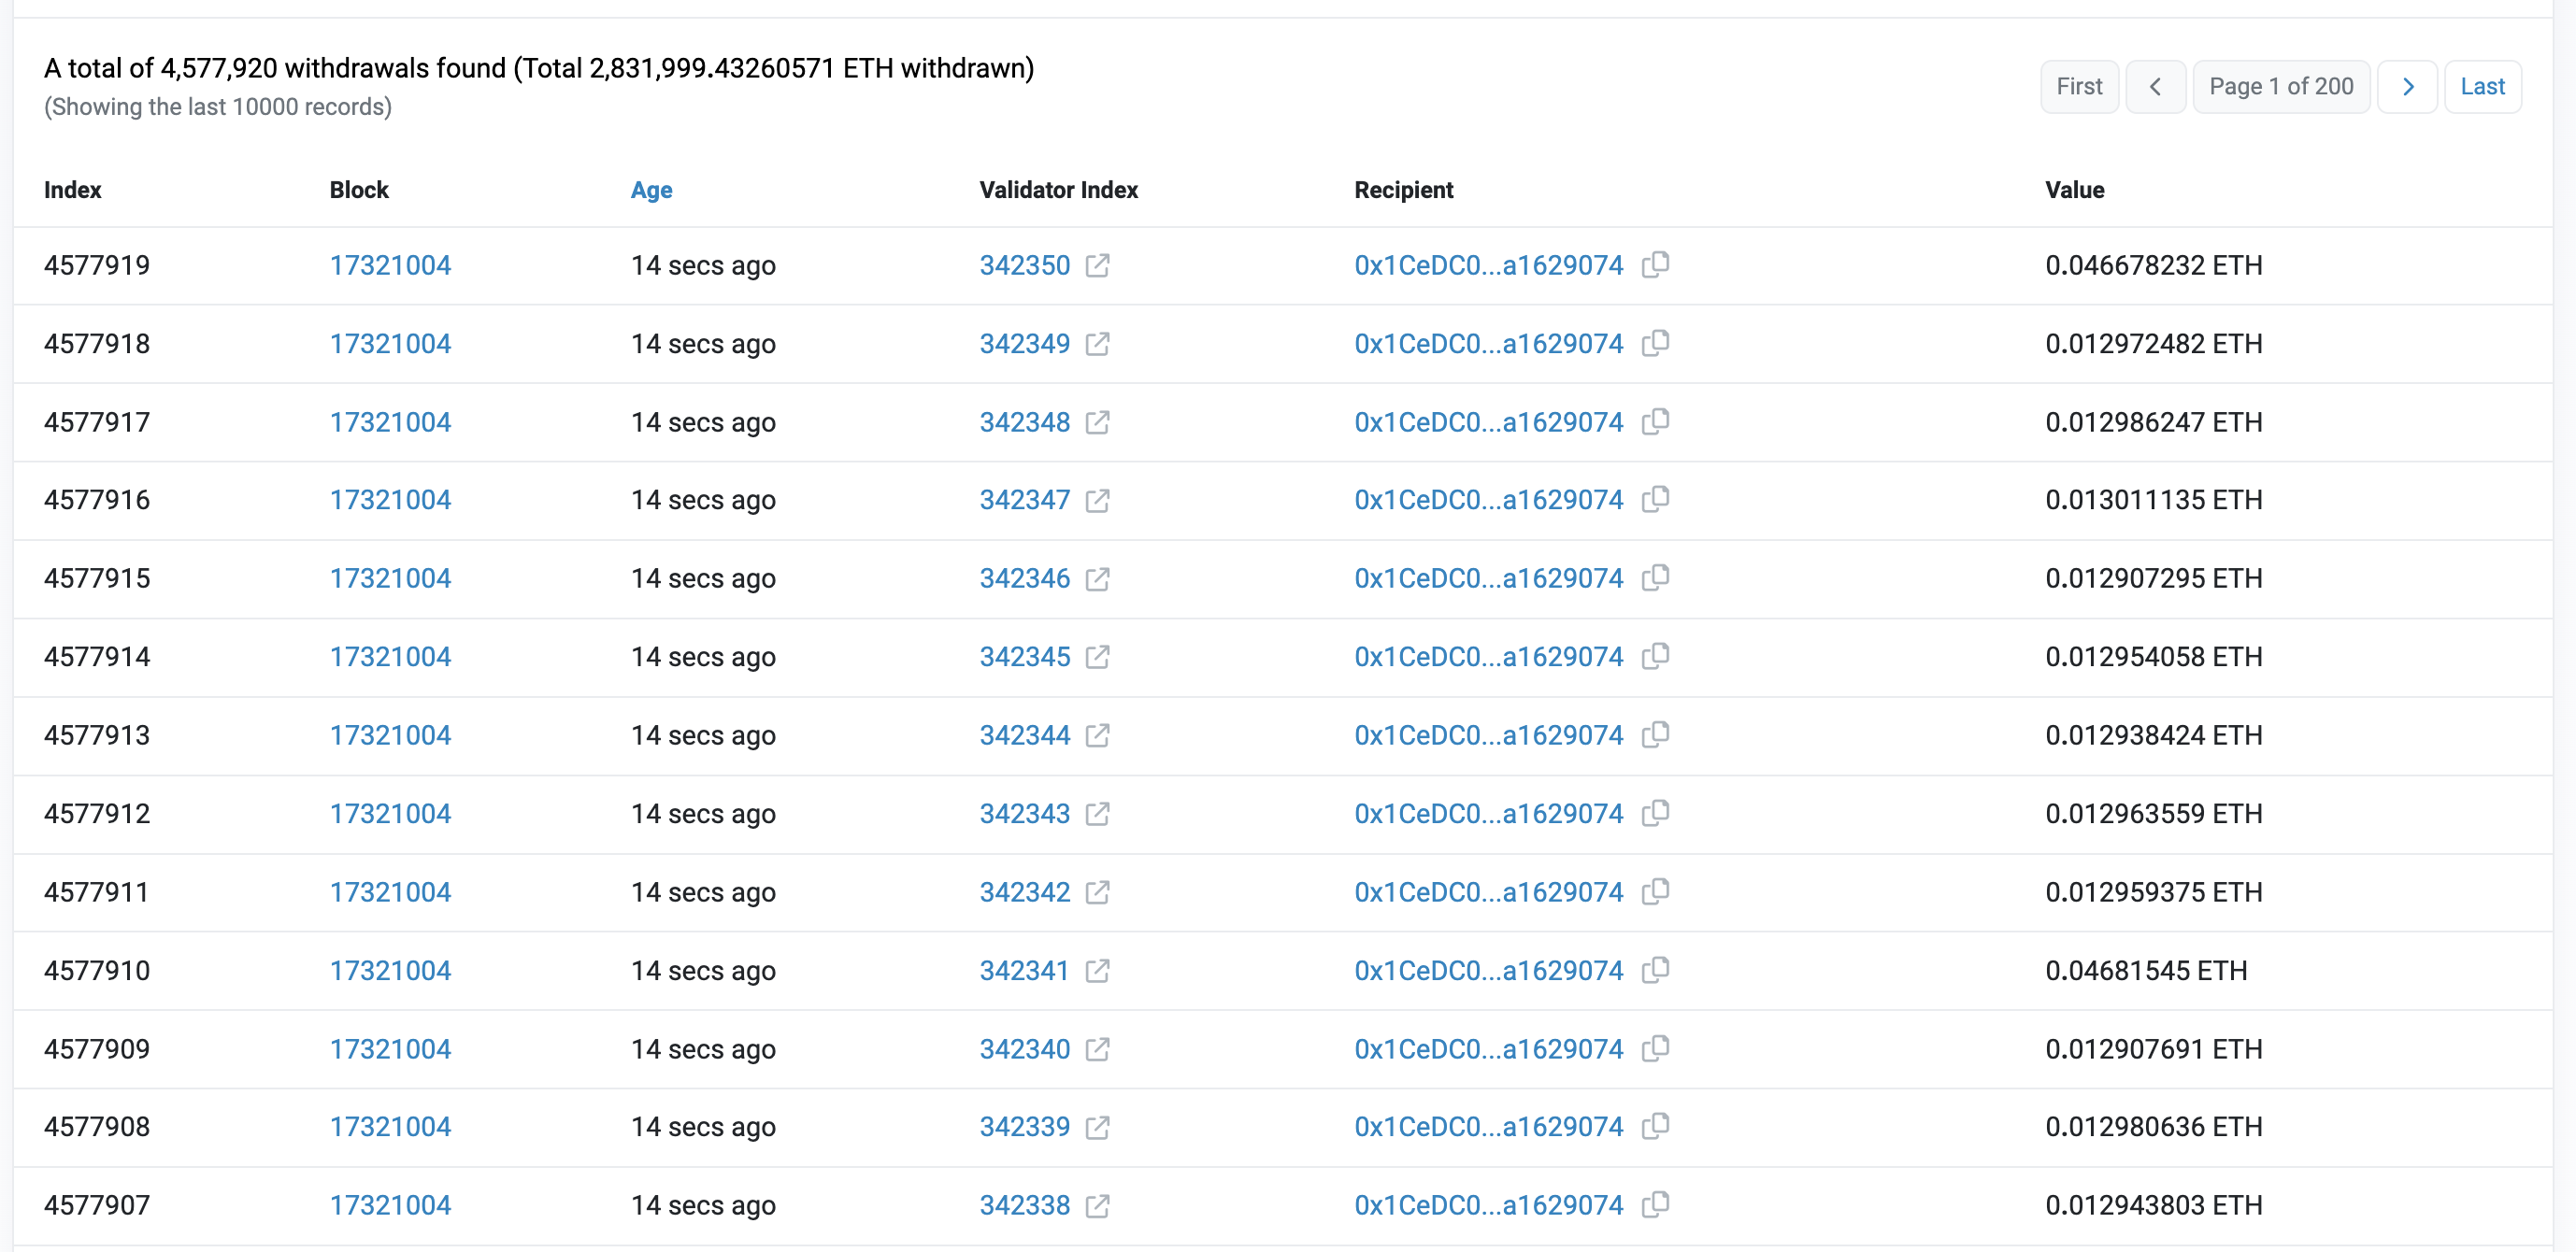
\includegraphics[width=0.48\linewidth]{images/withdrawals} \\
(a)\hspace{160pt}        (b)\\
\caption{Beacon chain deposits (a) and withdrawals (b) from Etherscan (23 May 2023)}
\label{fig:deposits}
\end{center}
\end{figure}

\begin{figure}[htbp]
\begin{center}
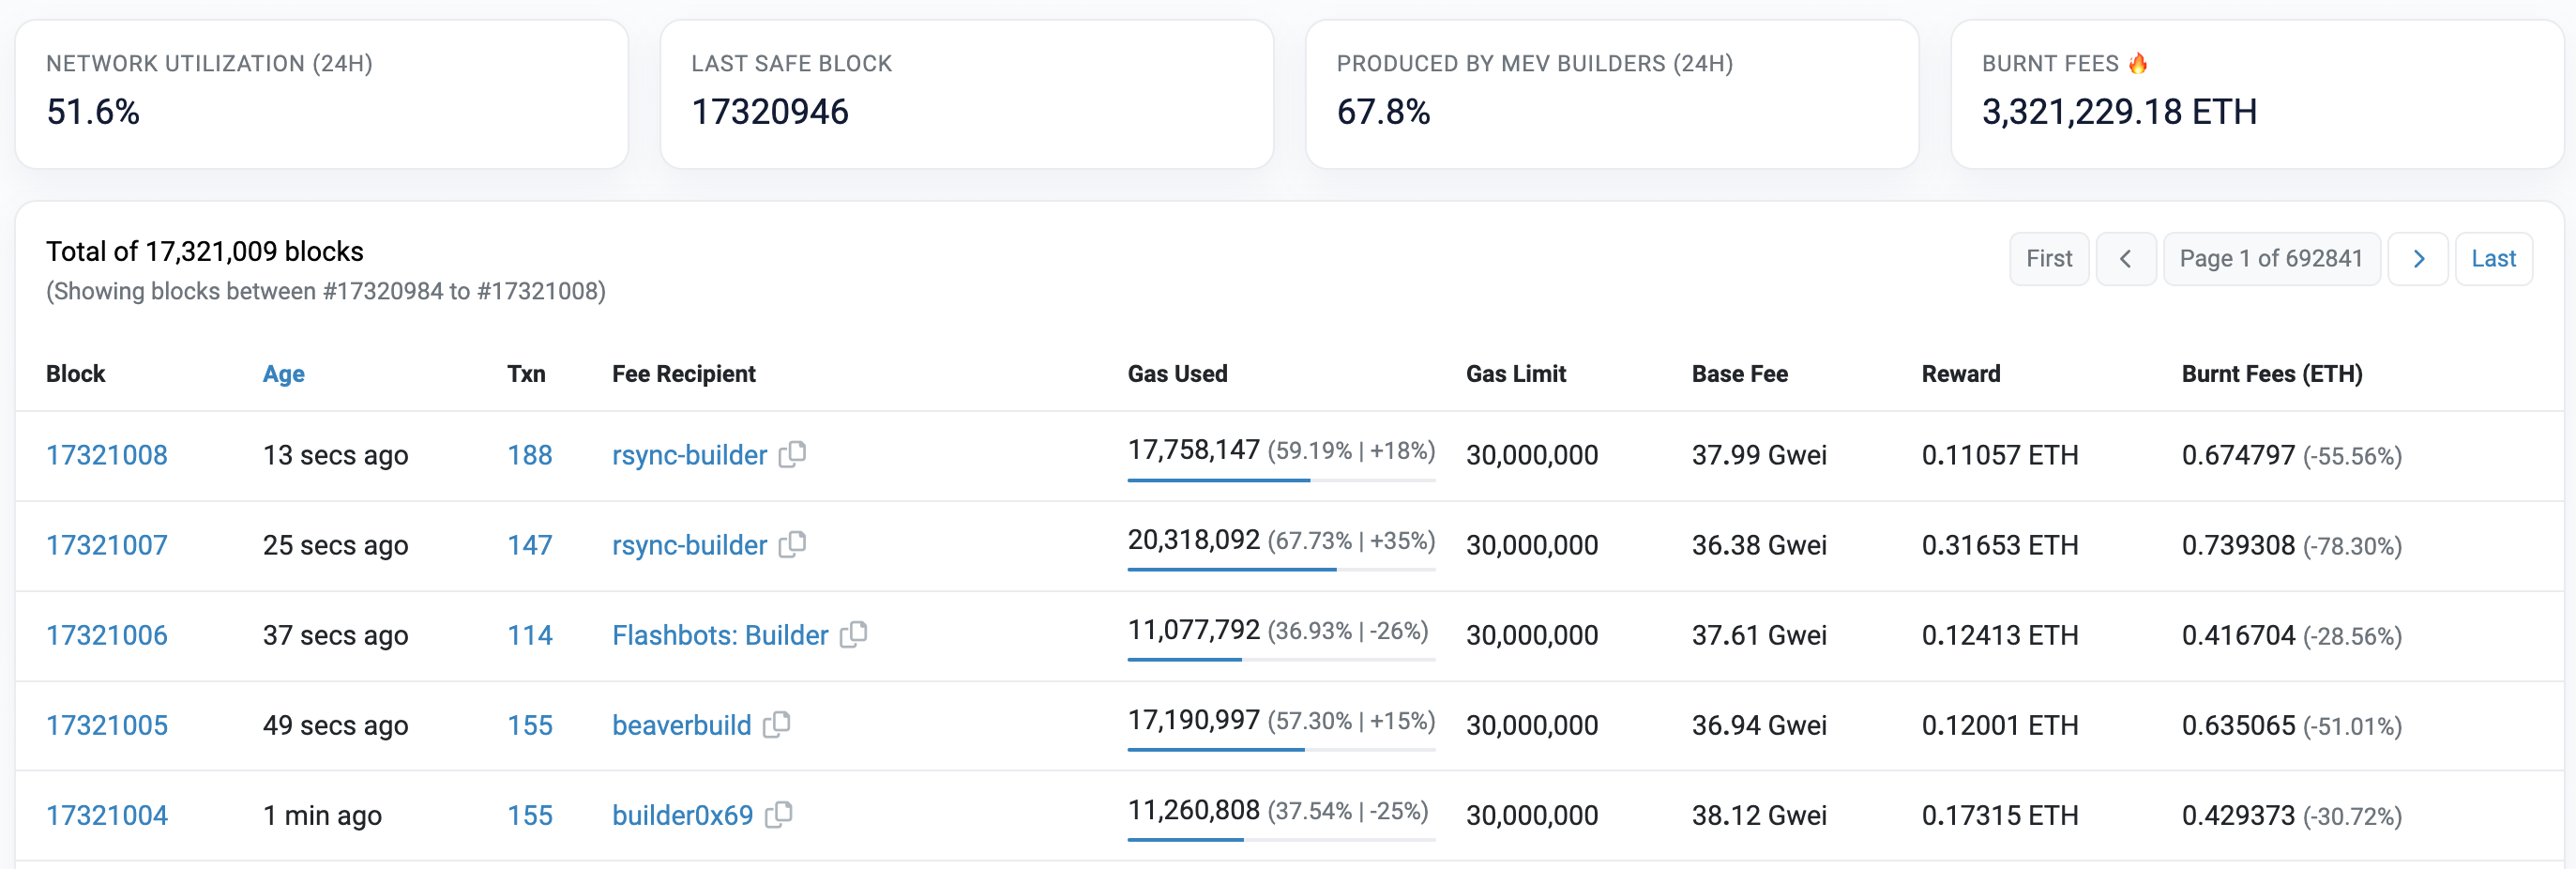
\includegraphics[width=0.48\linewidth]{images/blocks}
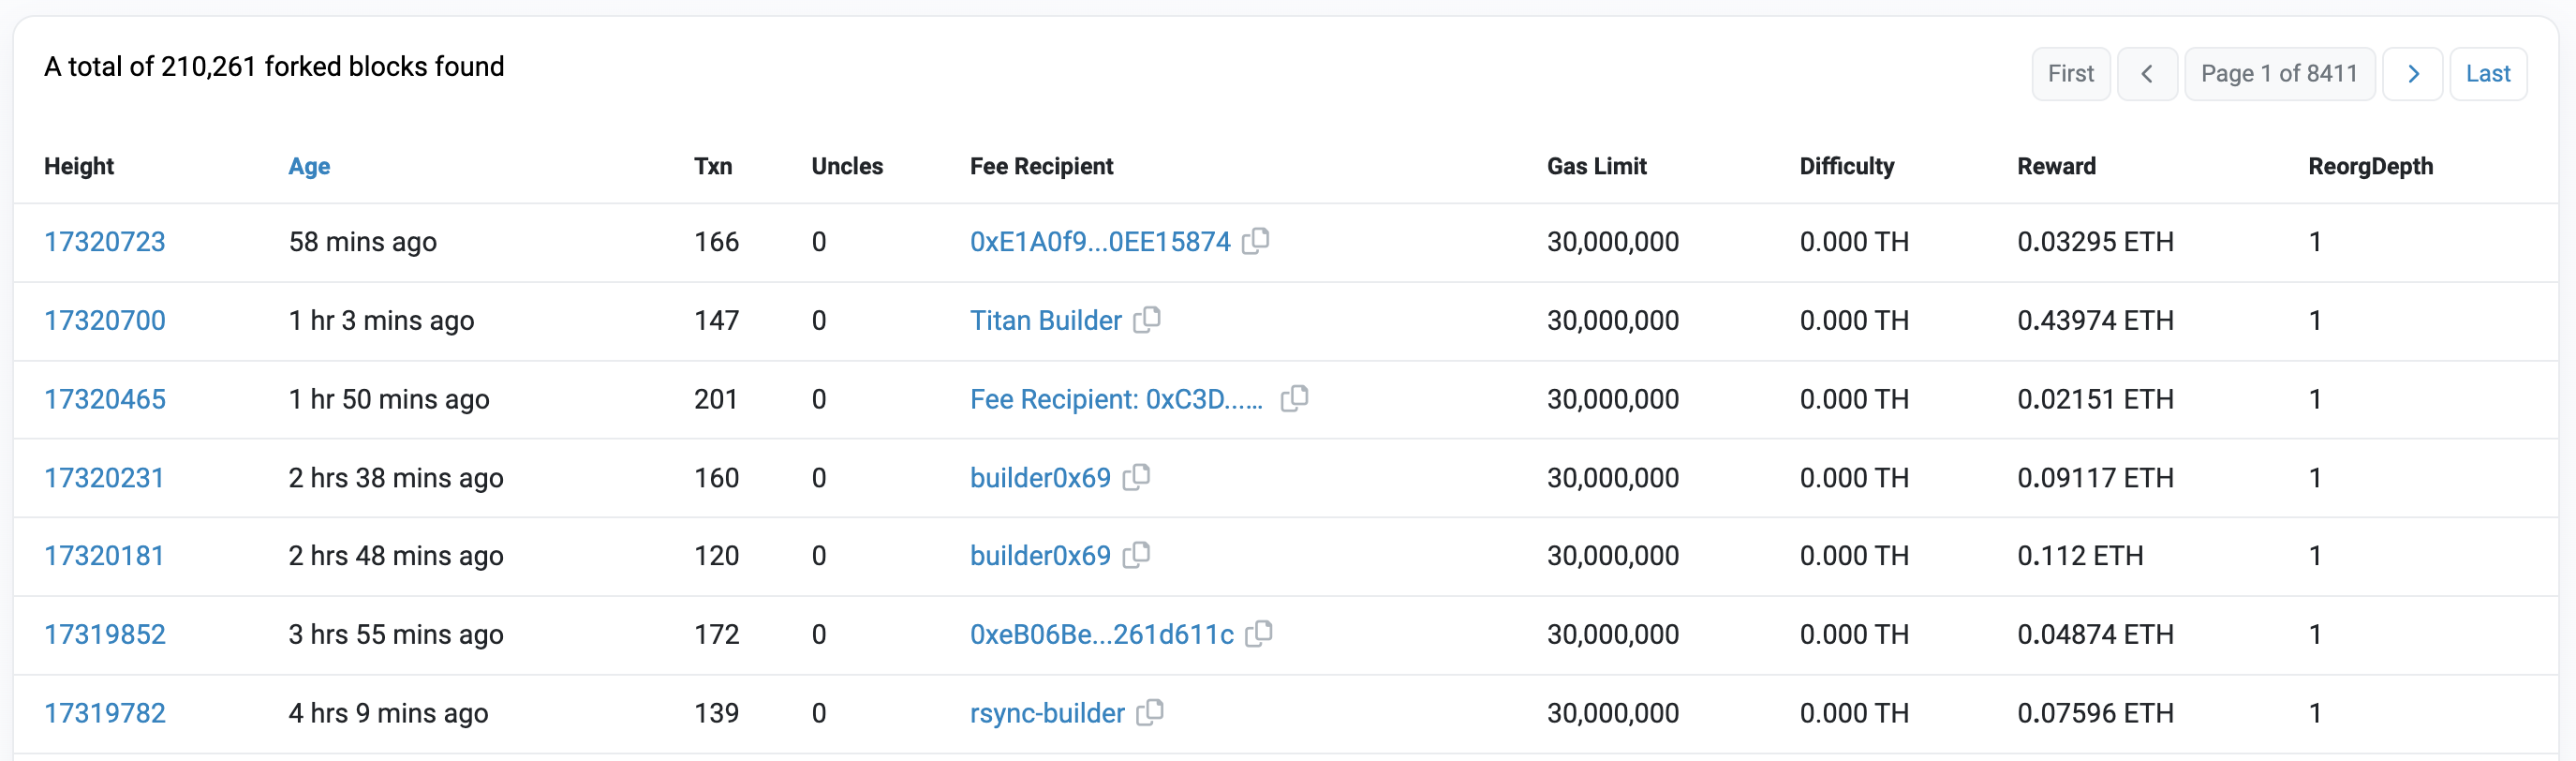
\includegraphics[width=0.48\linewidth]{images/forked} \\
(a)\hspace{160pt}        (b)\\
\caption{Details of beacon chain blocks (a) and forked blocks (b) from Etherscan (23 May 2023)}
\label{fig:blocks}
\end{center}
\end{figure}

\begin{figure}[htbp]
\begin{center}
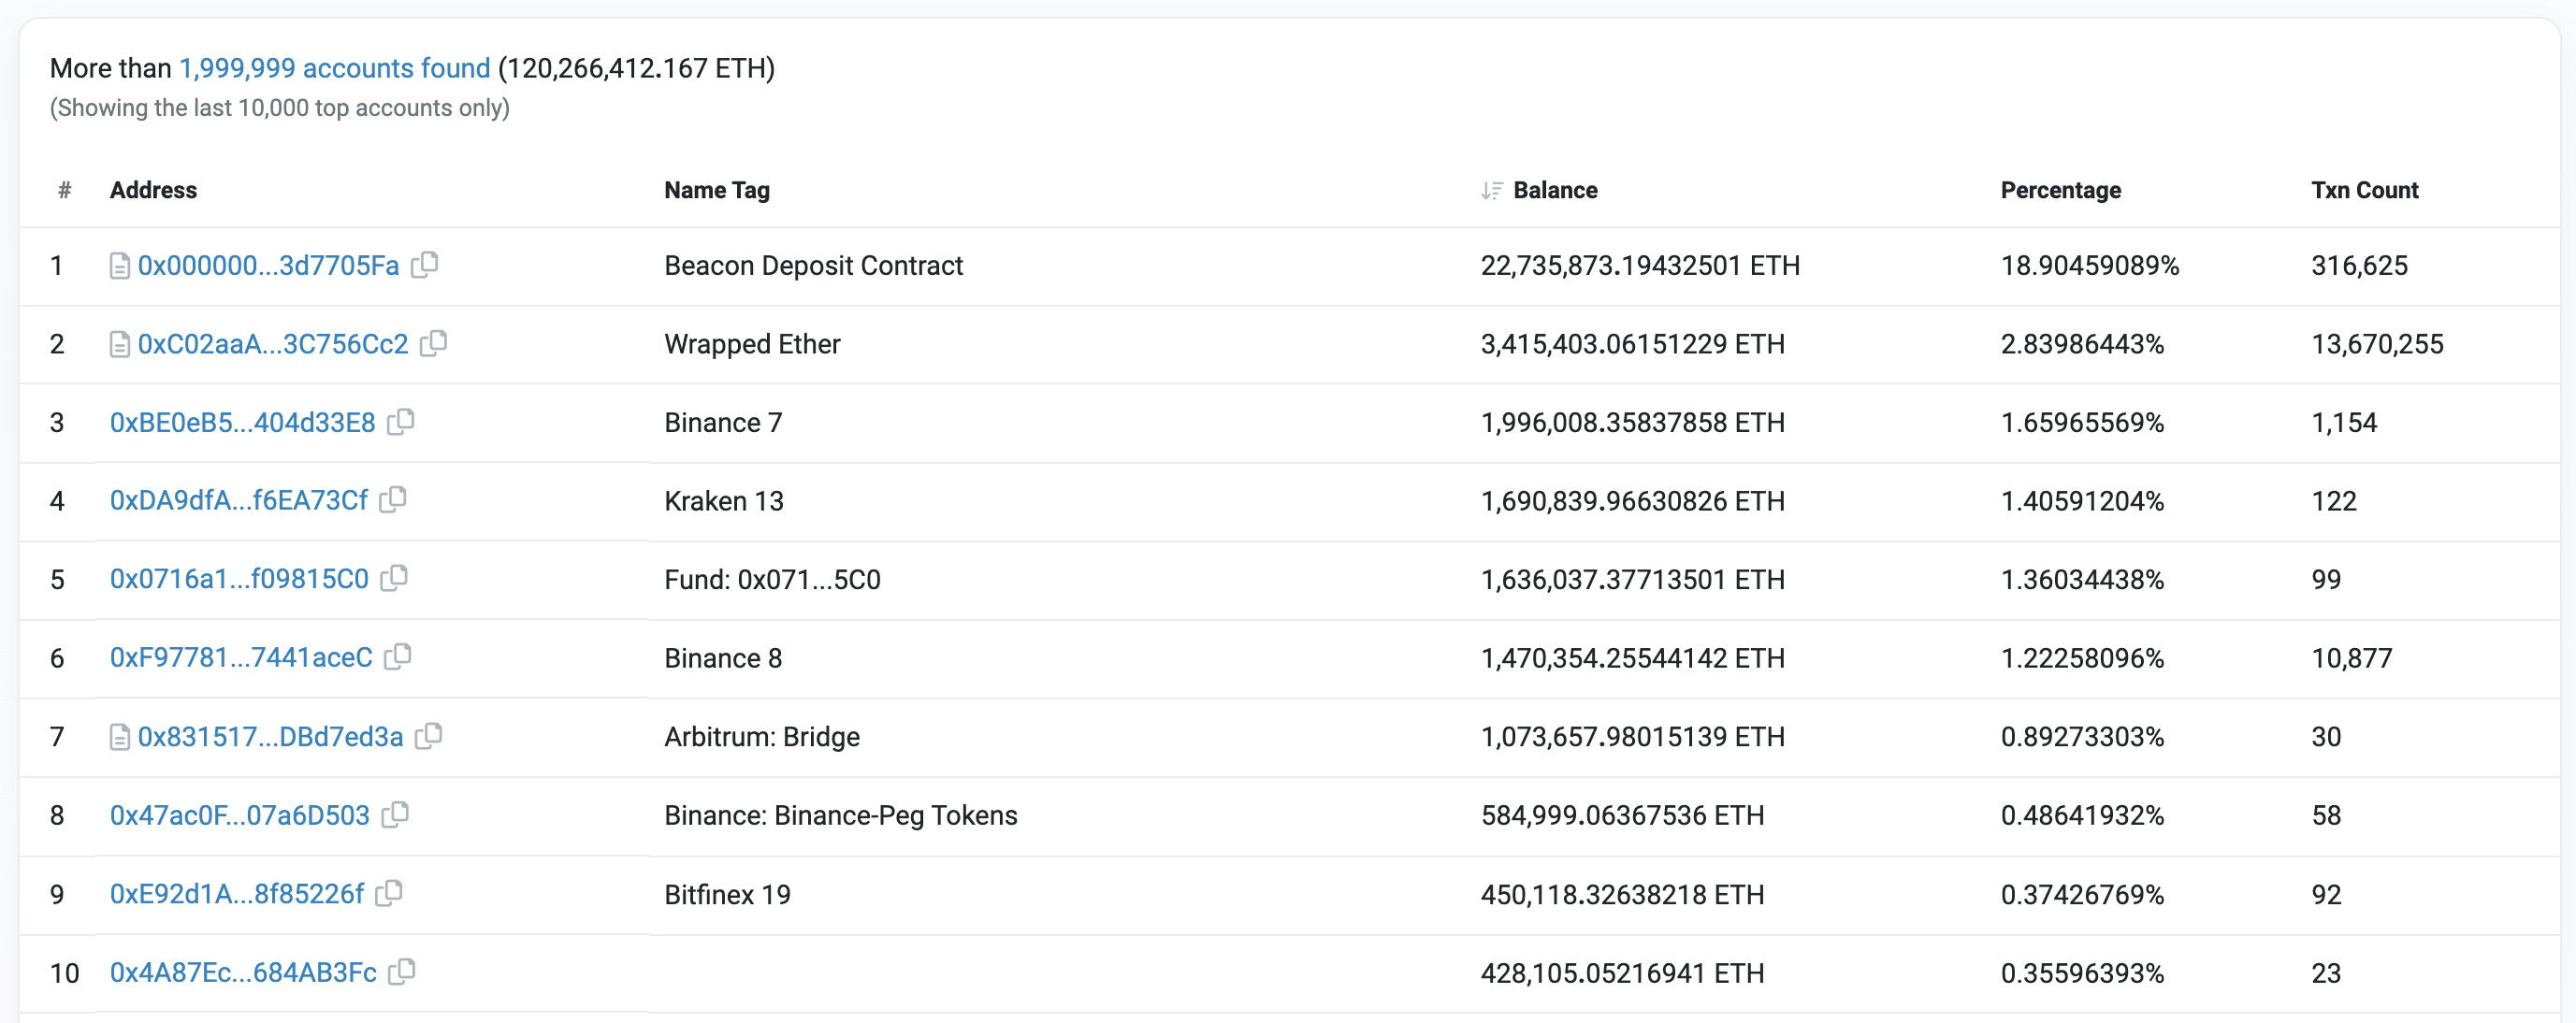
\includegraphics[width=0.48\linewidth]{images/accounts}
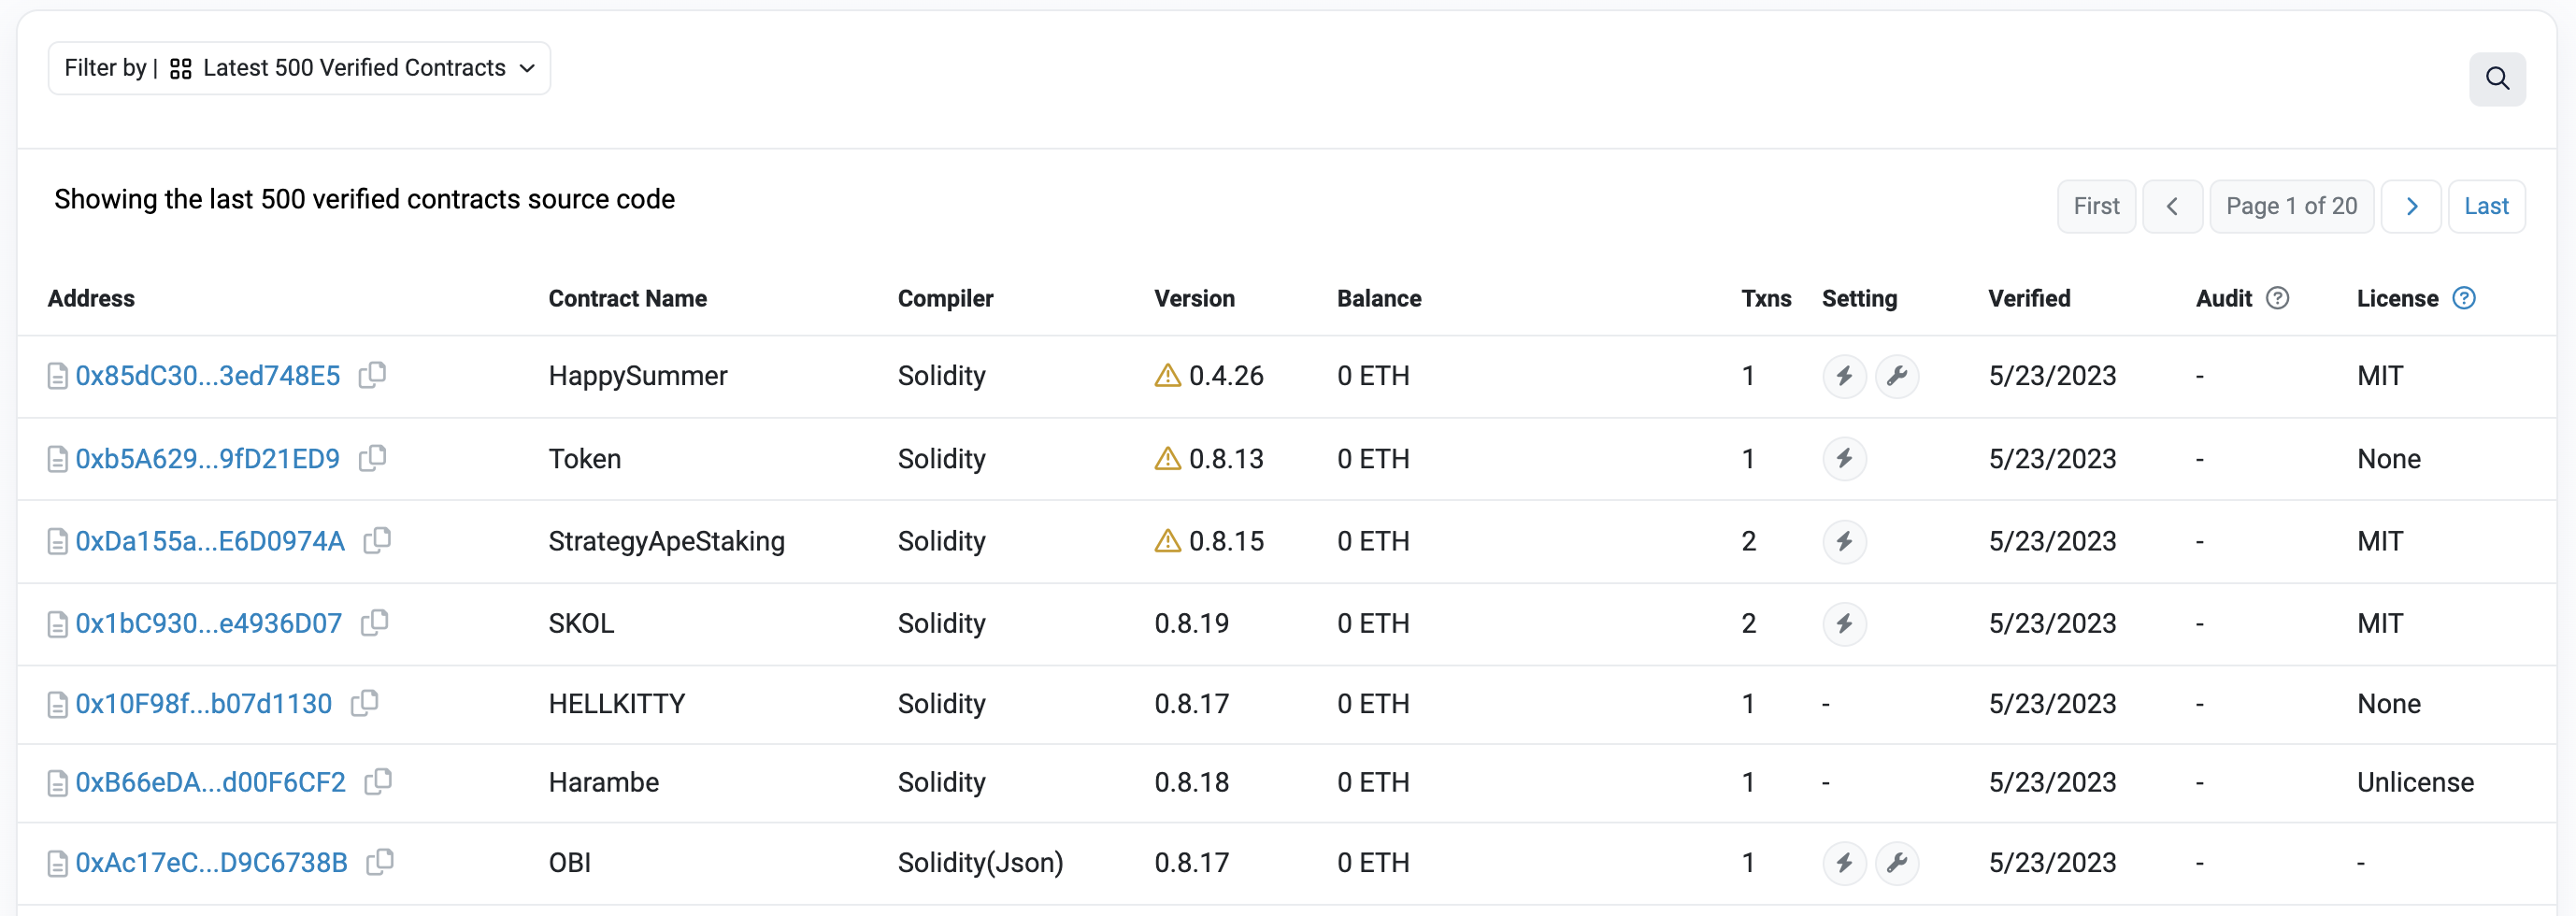
\includegraphics[width=0.48\linewidth]{images/contracts} \\
(a)\hspace{160pt}        (b)\\
\caption{Top accounts by ETH balance (a) and verified contract source code (b) from Etherscan (23 May 2023)}
\label{fig:accounts}
\end{center}
\end{figure}

\begin{figure}[htbp]
\begin{center}
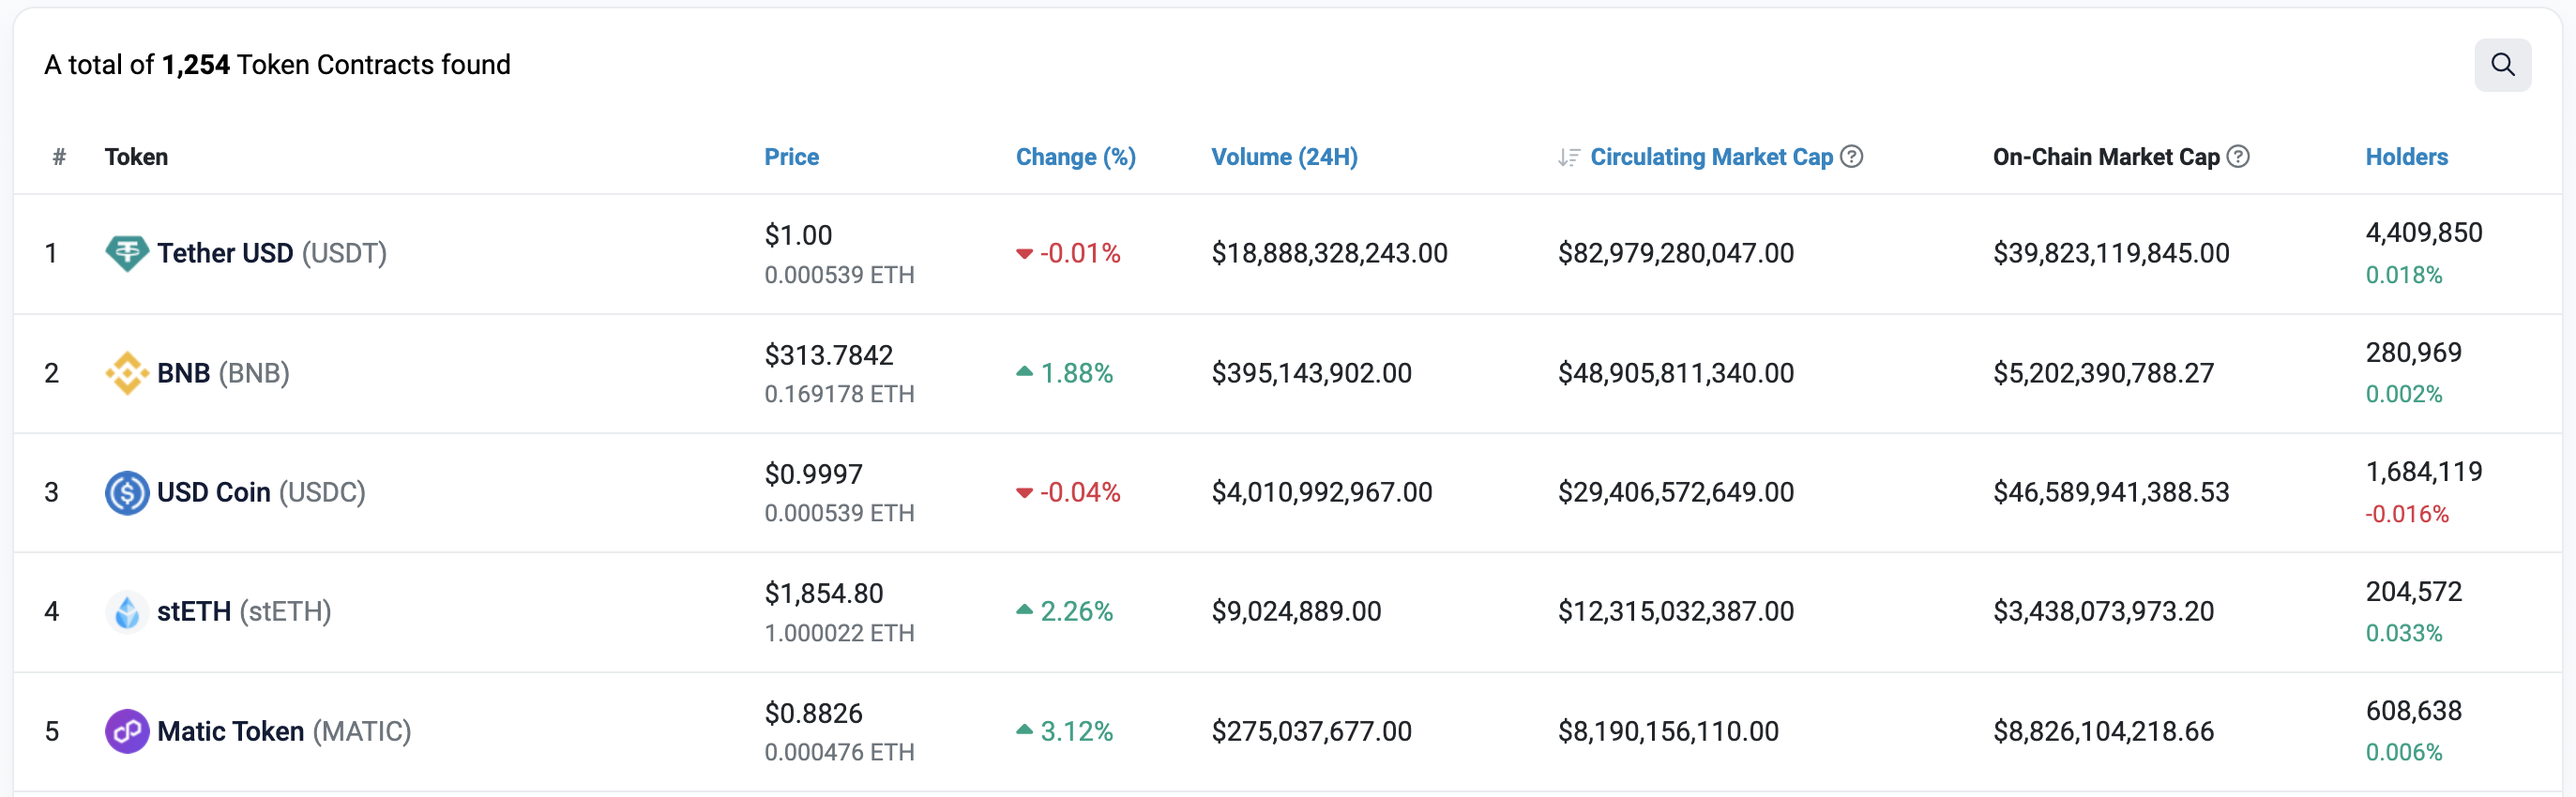
\includegraphics[width=0.48\linewidth]{images/erc20}
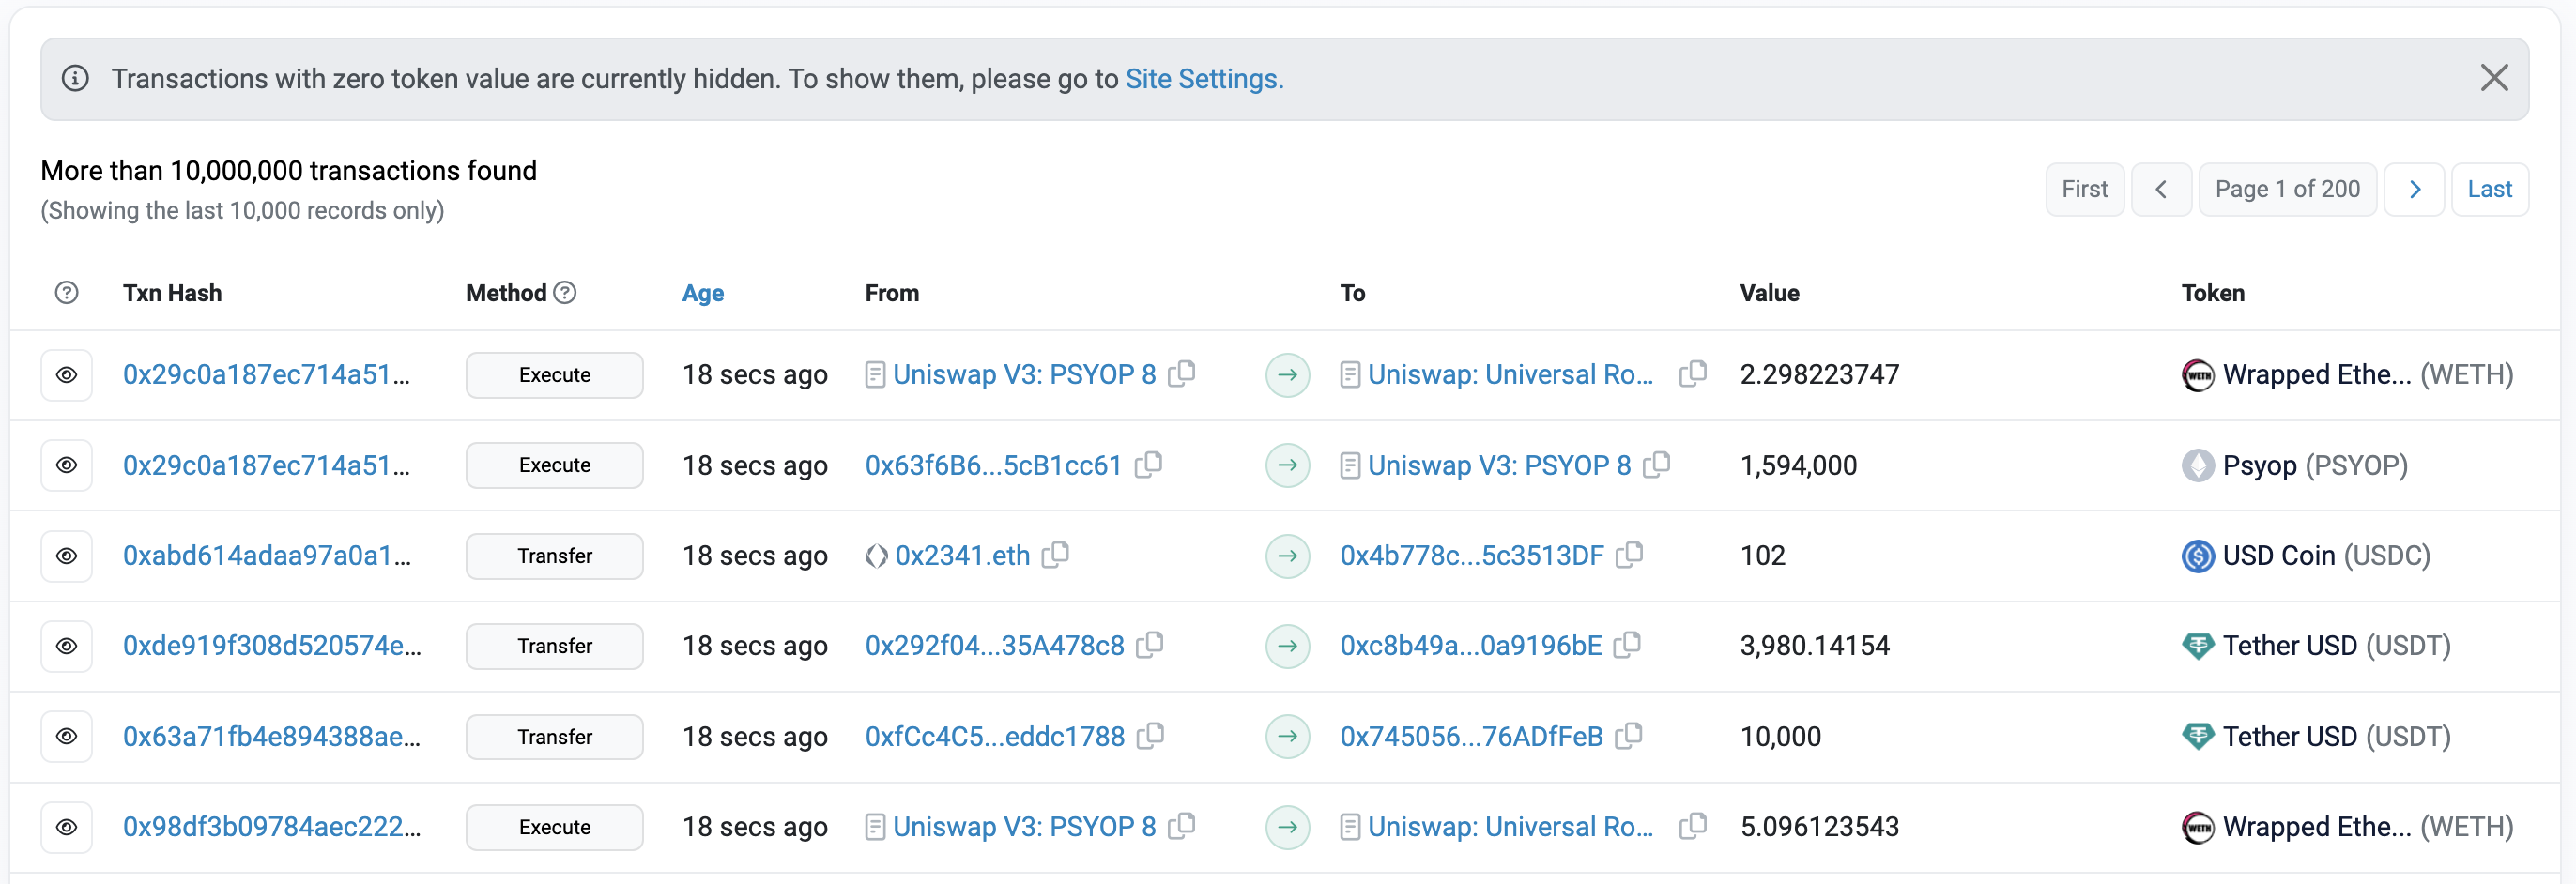
\includegraphics[width=0.48\linewidth]{images/xfrs} \\
(a)\hspace{160pt}        (b)\\
\caption{Top ERC20 tokens (a) and ERC20 token transfers (b) from Etherscan (23 May 2023)}
\label{fig:erc20}
\end{center}
\end{figure}

\clearpage
\textbf{Charts and Statistics}\\
% -------------------------------------

\begin{figure}[htbp]
\begin{center}
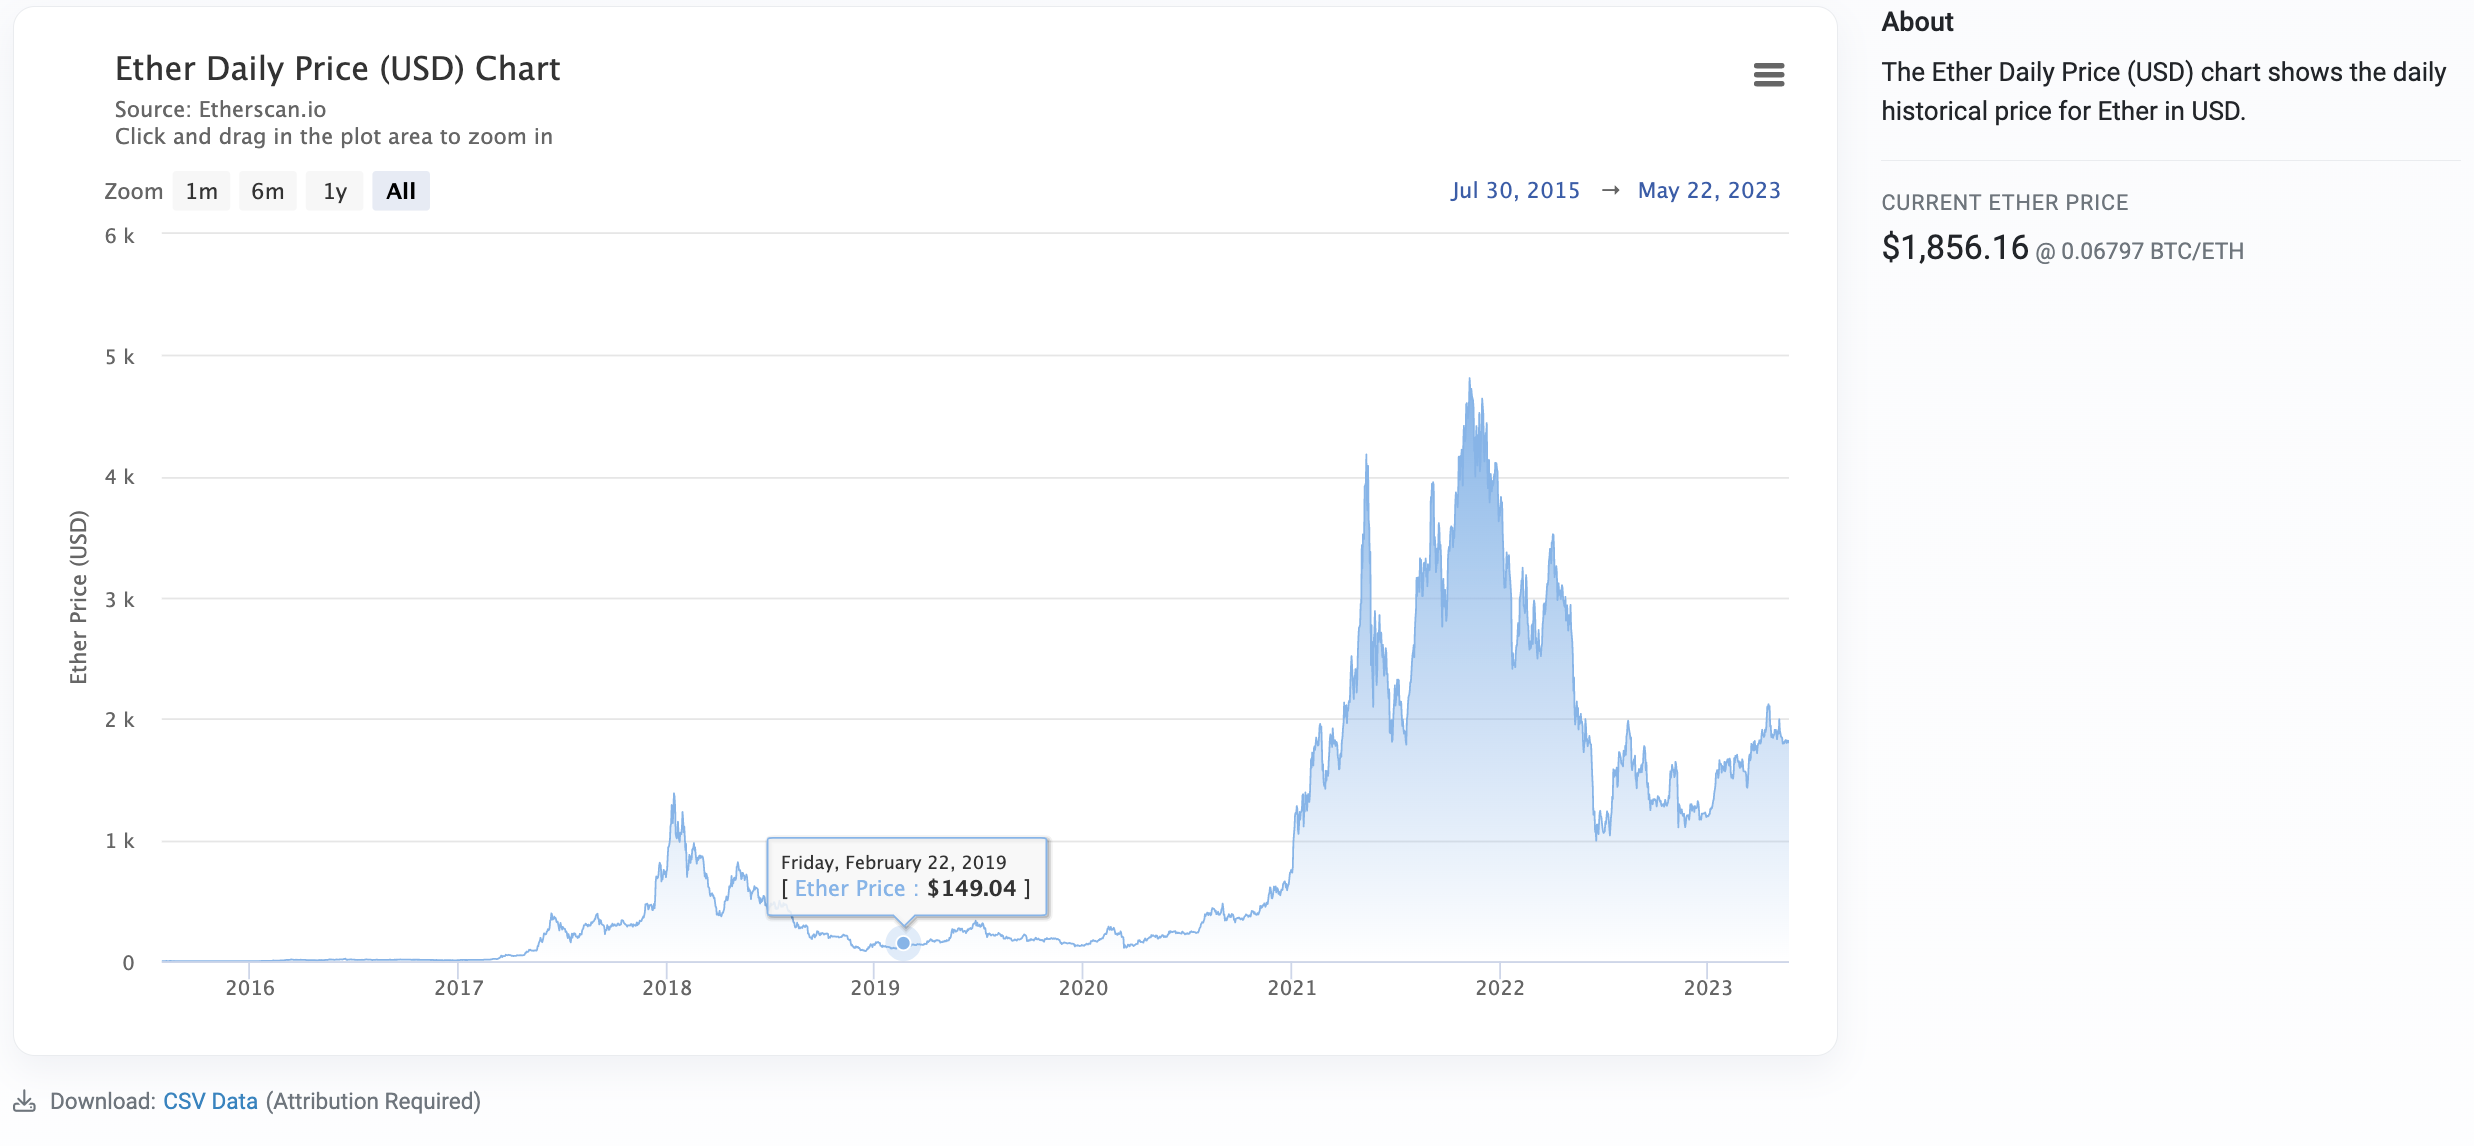
\includegraphics[width=0.9\linewidth]{images/ethdaily}
\caption{Ether daily price (USD) from Etherscan, 23 May 2023}
\label{fig:ethdaily}
\end{center}
\end{figure}

\begin{figure}[htbp]
\begin{center}
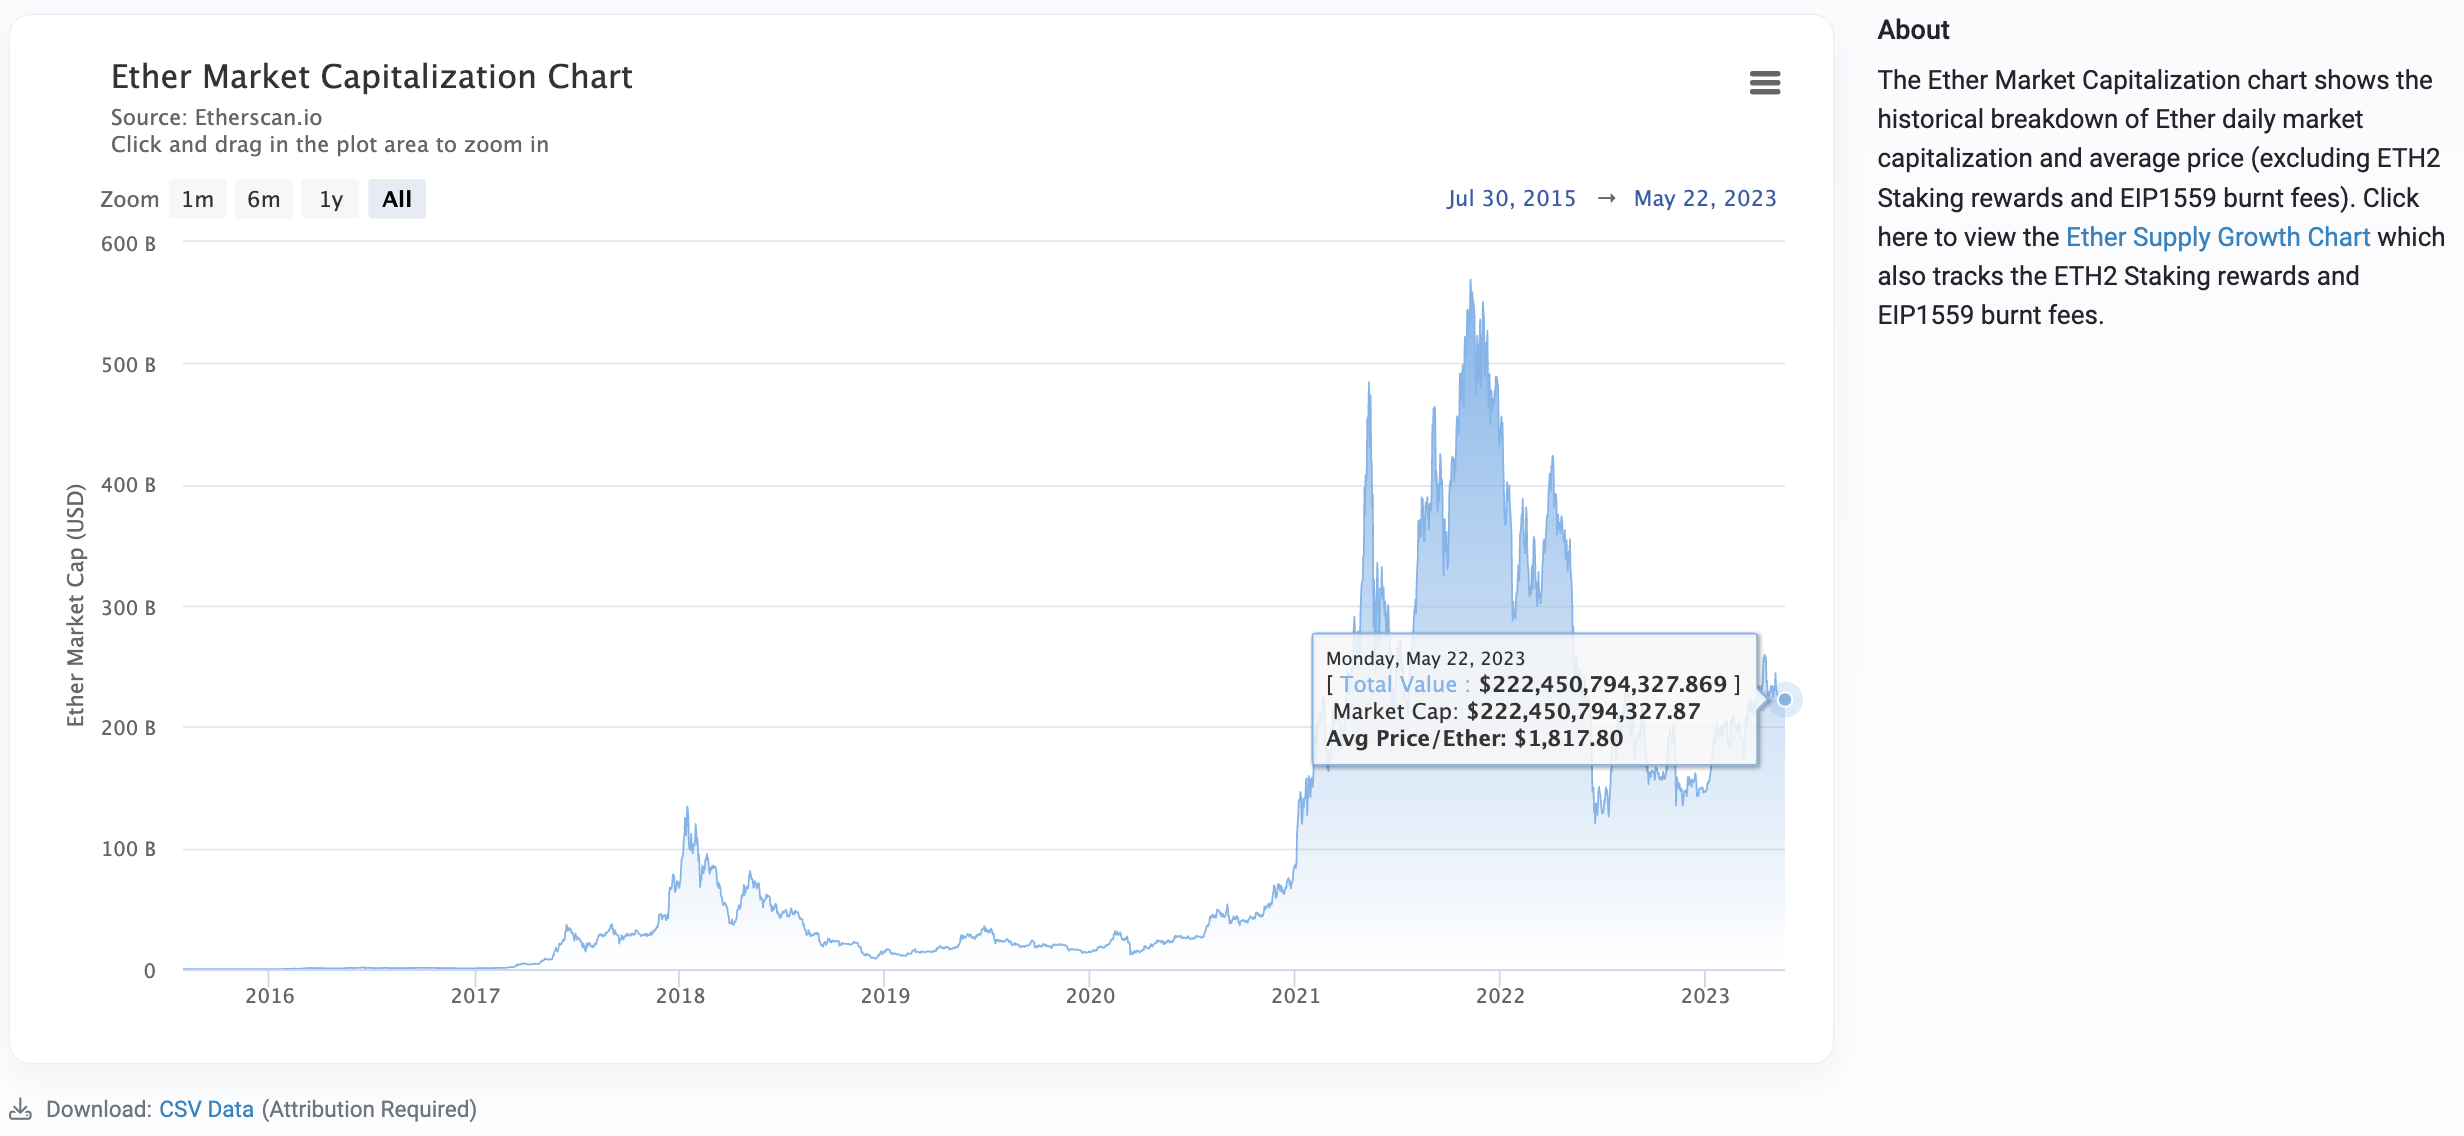
\includegraphics[width=0.9\linewidth]{images/marketcap}
\caption{Ether market capitalisation from Etherscan  - select time range or zoom in on selected part of graph, hover mouse for details (as shown), 23 May 2023}
\label{fig:marketcap}
\end{center}
\end{figure}

\begin{figure}[htbp]
\begin{center}
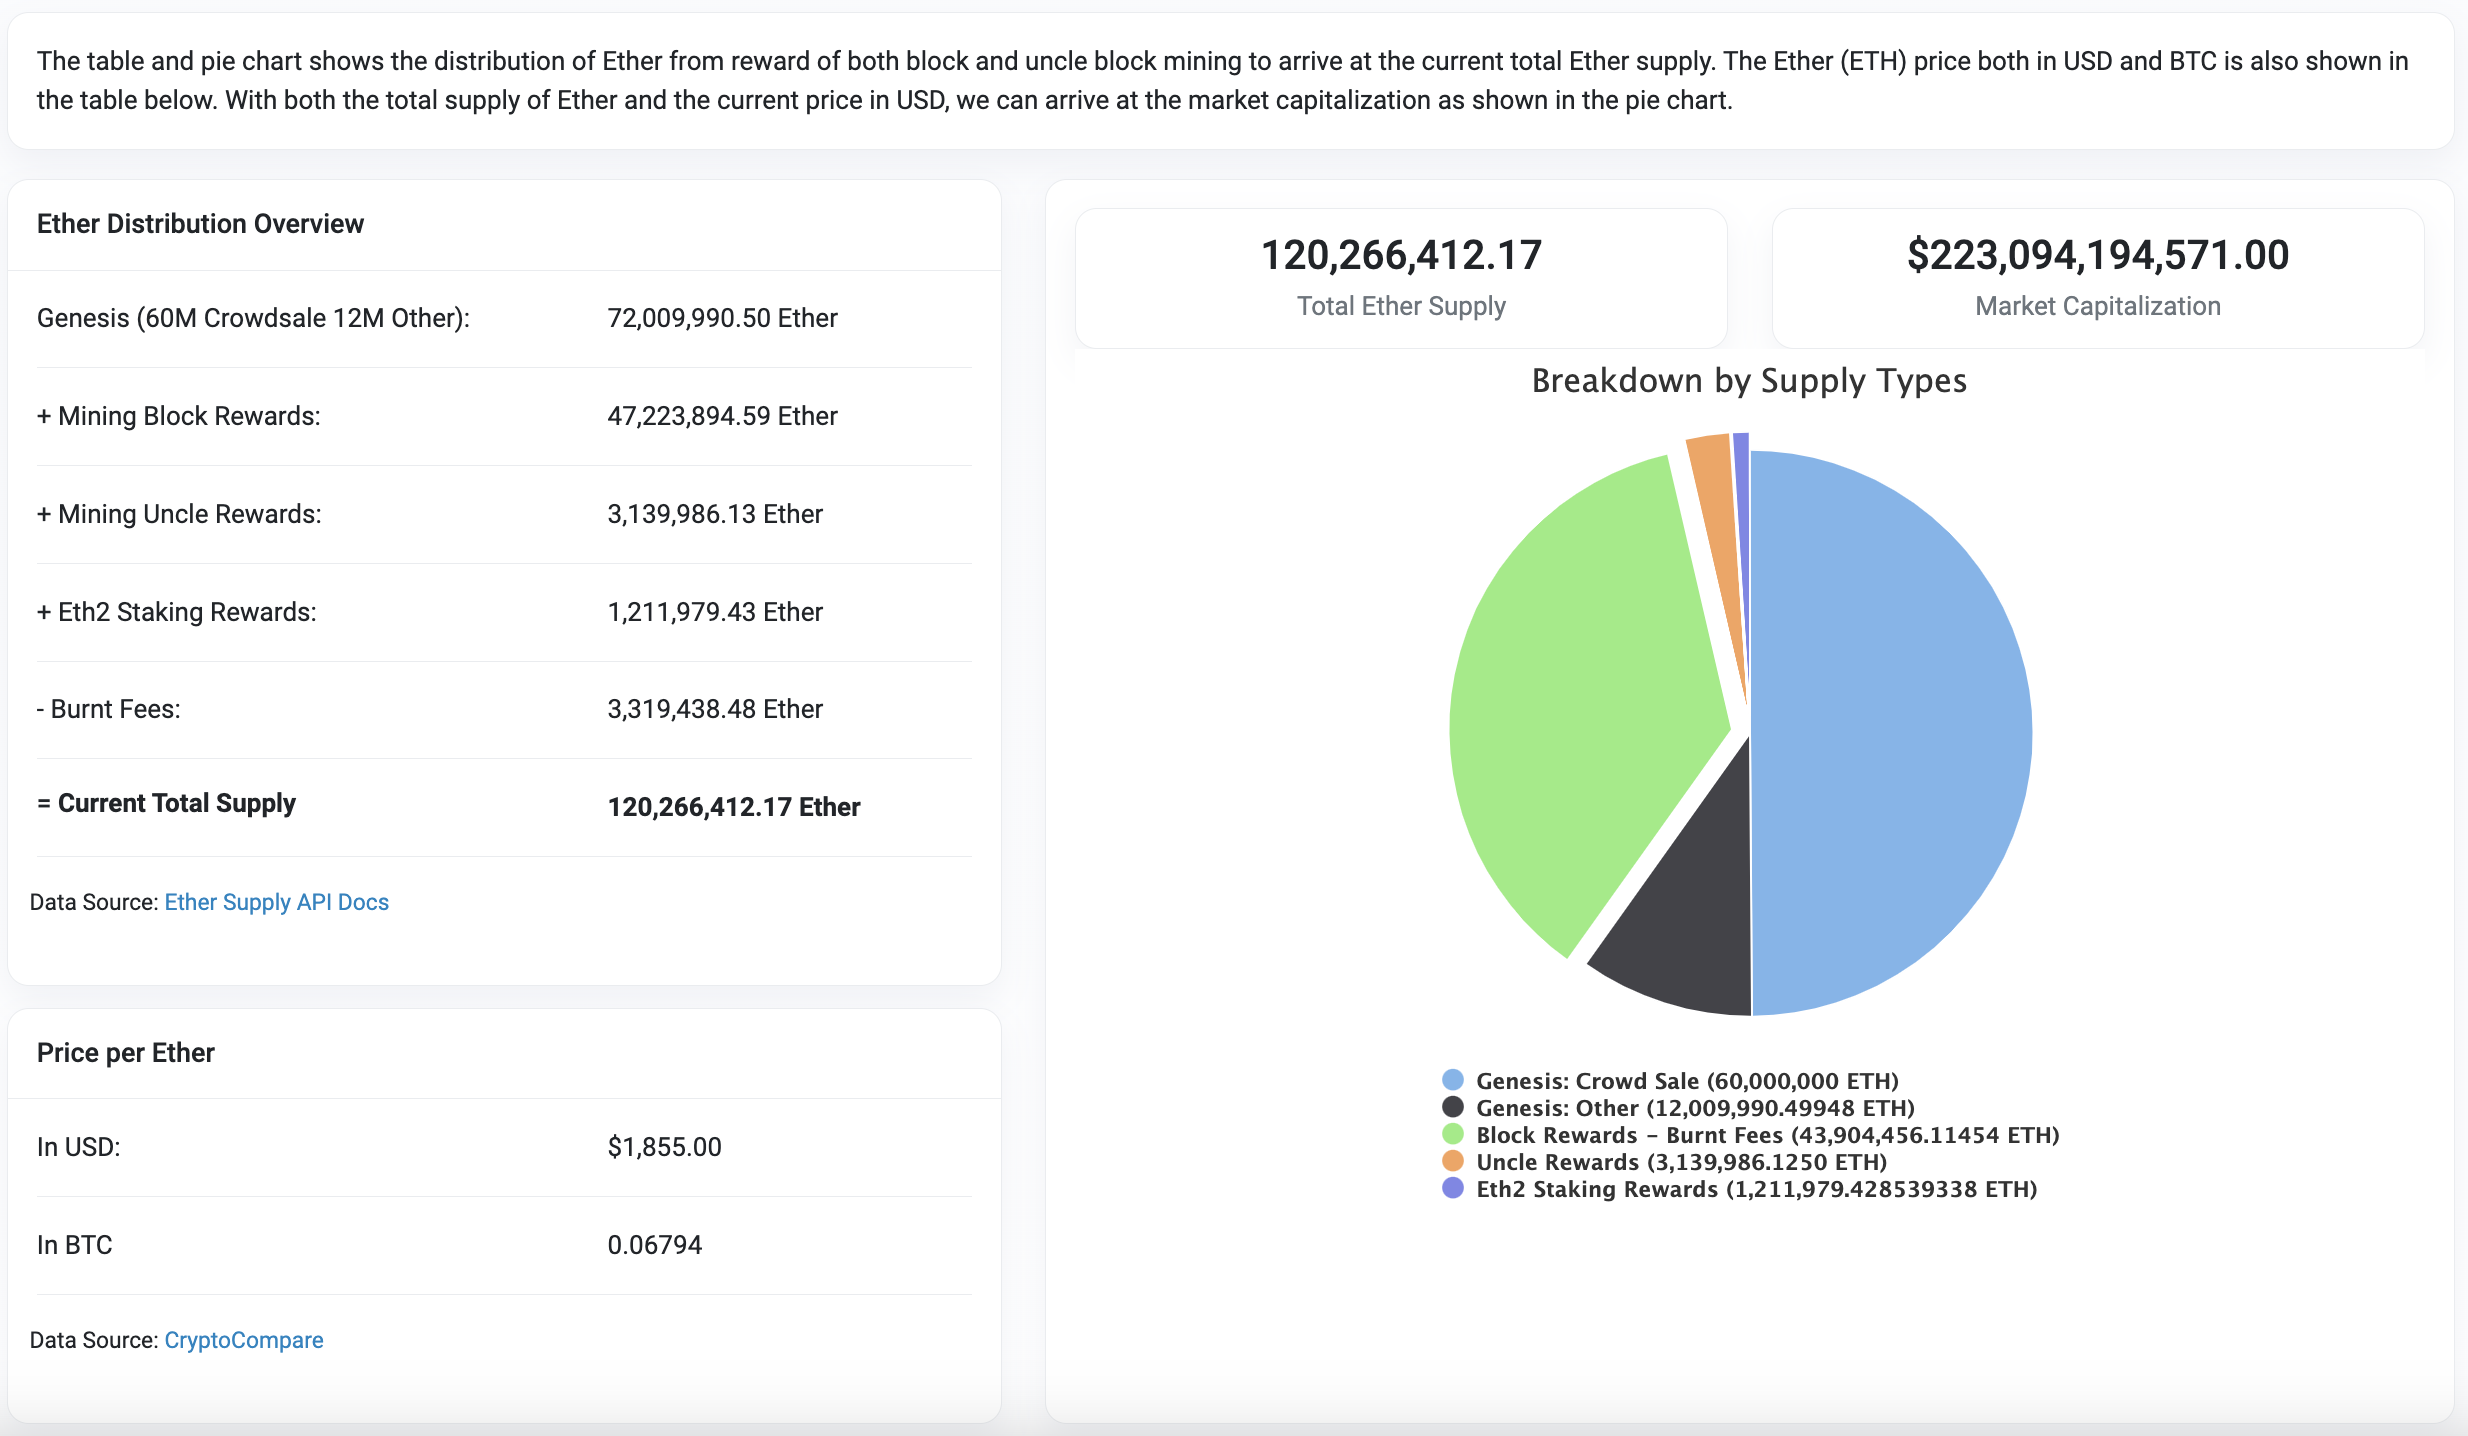
\includegraphics[width=0.9\linewidth]{images/totcap}
\caption{Ether total supply and market capitalisation from Etherscan, 23 May 2023}
\label{fig:totcap}
\end{center}
\end{figure}

\begin{figure}[htbp]
\begin{center}
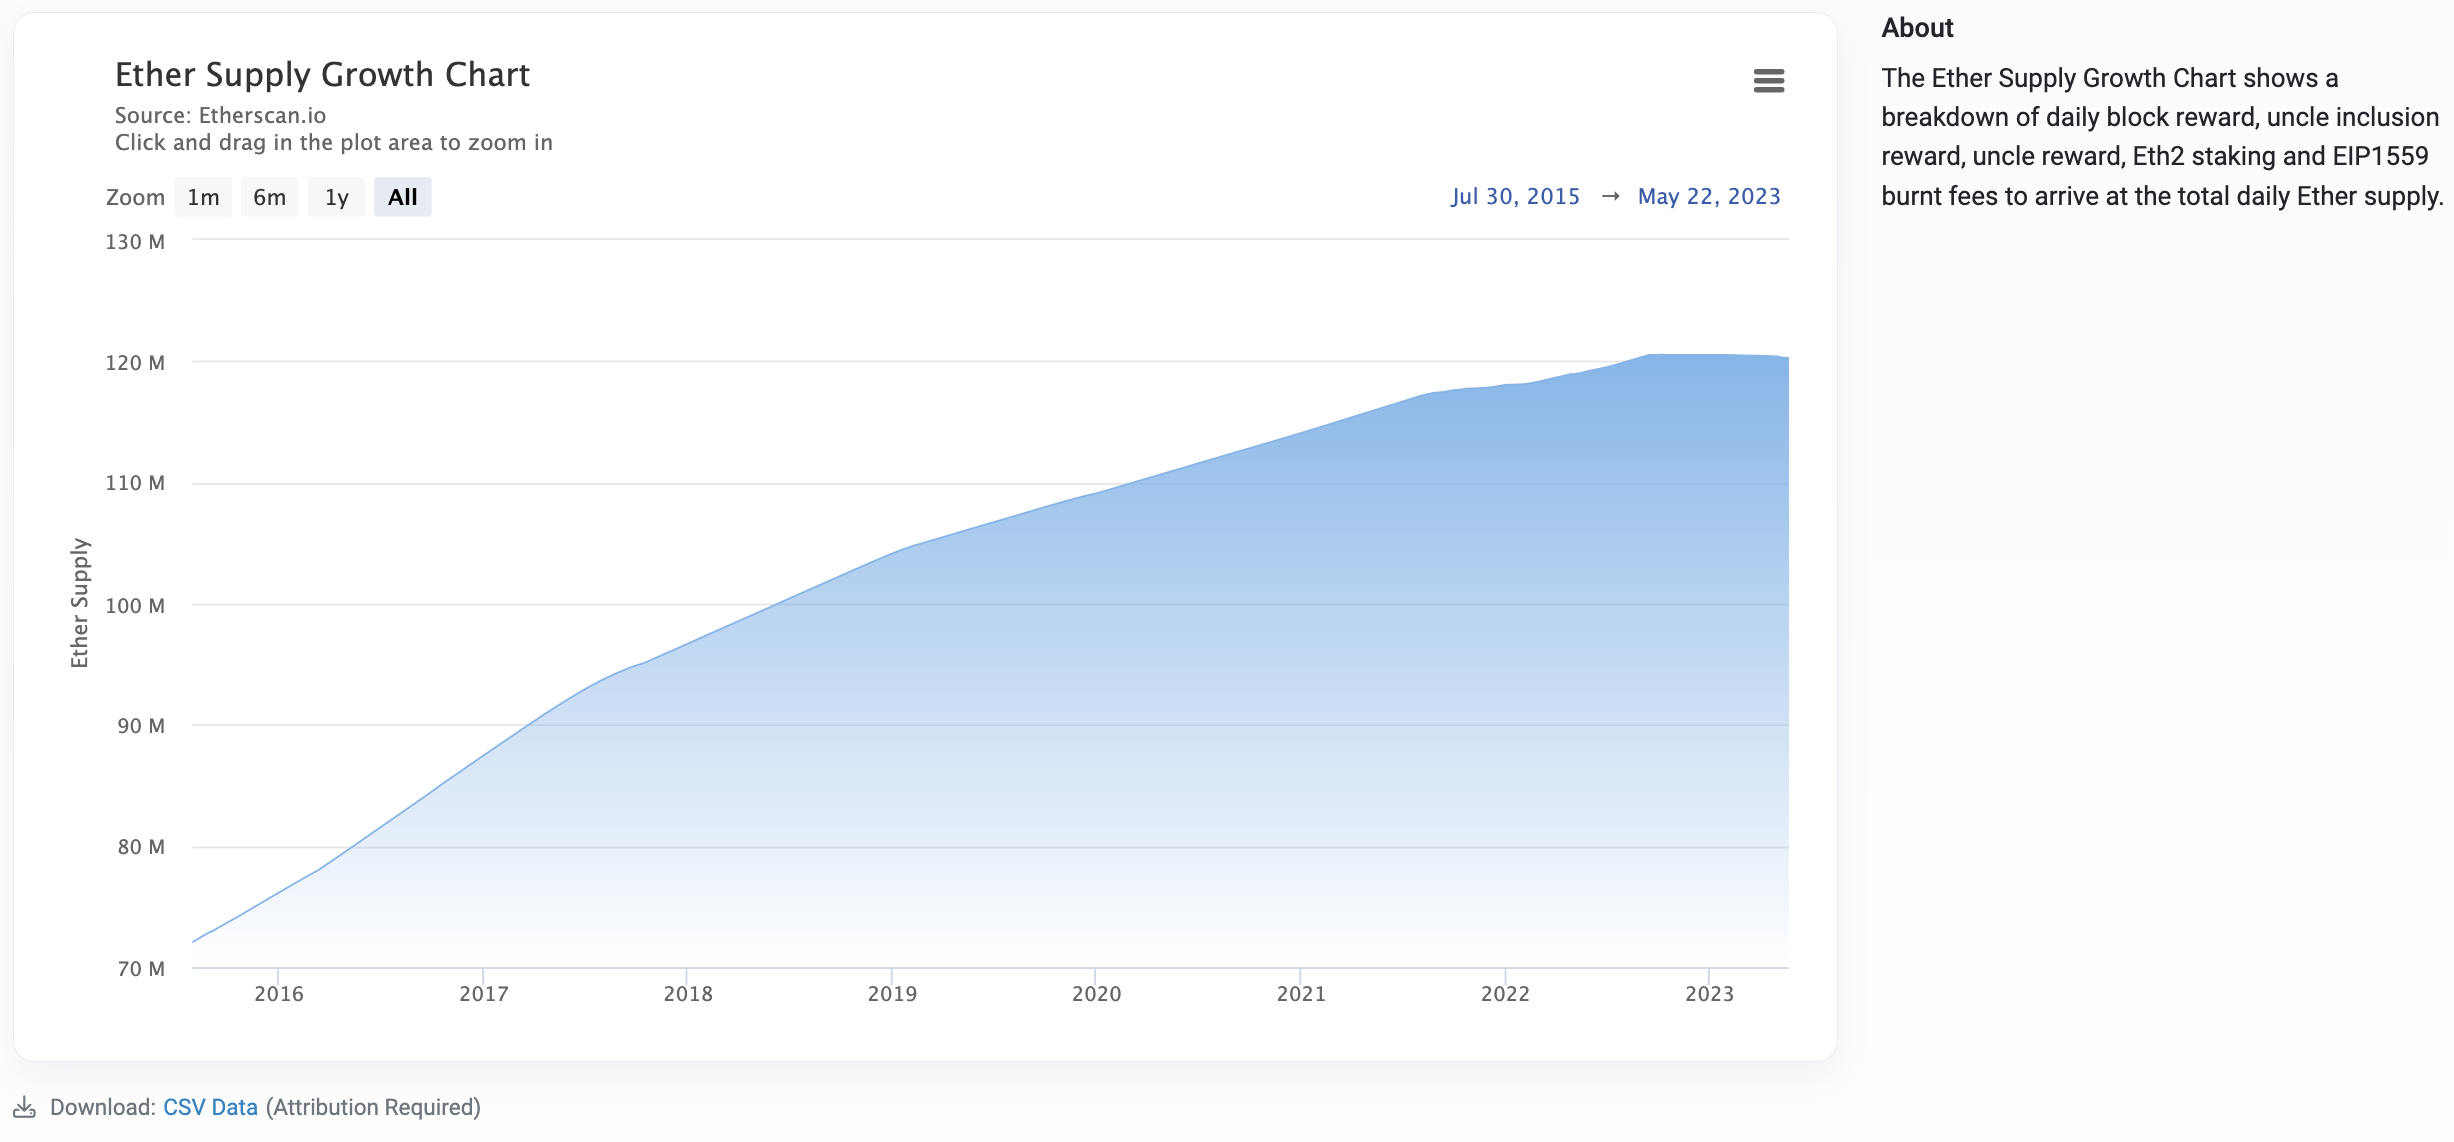
\includegraphics[width=0.9\linewidth]{images/ethgrowth}
\caption{Ether supply growth chart from Etherscan - select time range or zoom in on selected part of graph, 23 May 2023}
\label{fig:ethgrowth}
\end{center}
\end{figure}

\clearpage
% --------------------------------------
\subsubsection*{Beaconcha.in}
% --------------------------------------
The website provides the ability to search using a variety of fields, including a public key, block number, block graffiti, proposer, slot, and epoch. Apart from the extensive information and visualisations shown here, there are several other 

\begin{figure}[htbp]
\begin{center}
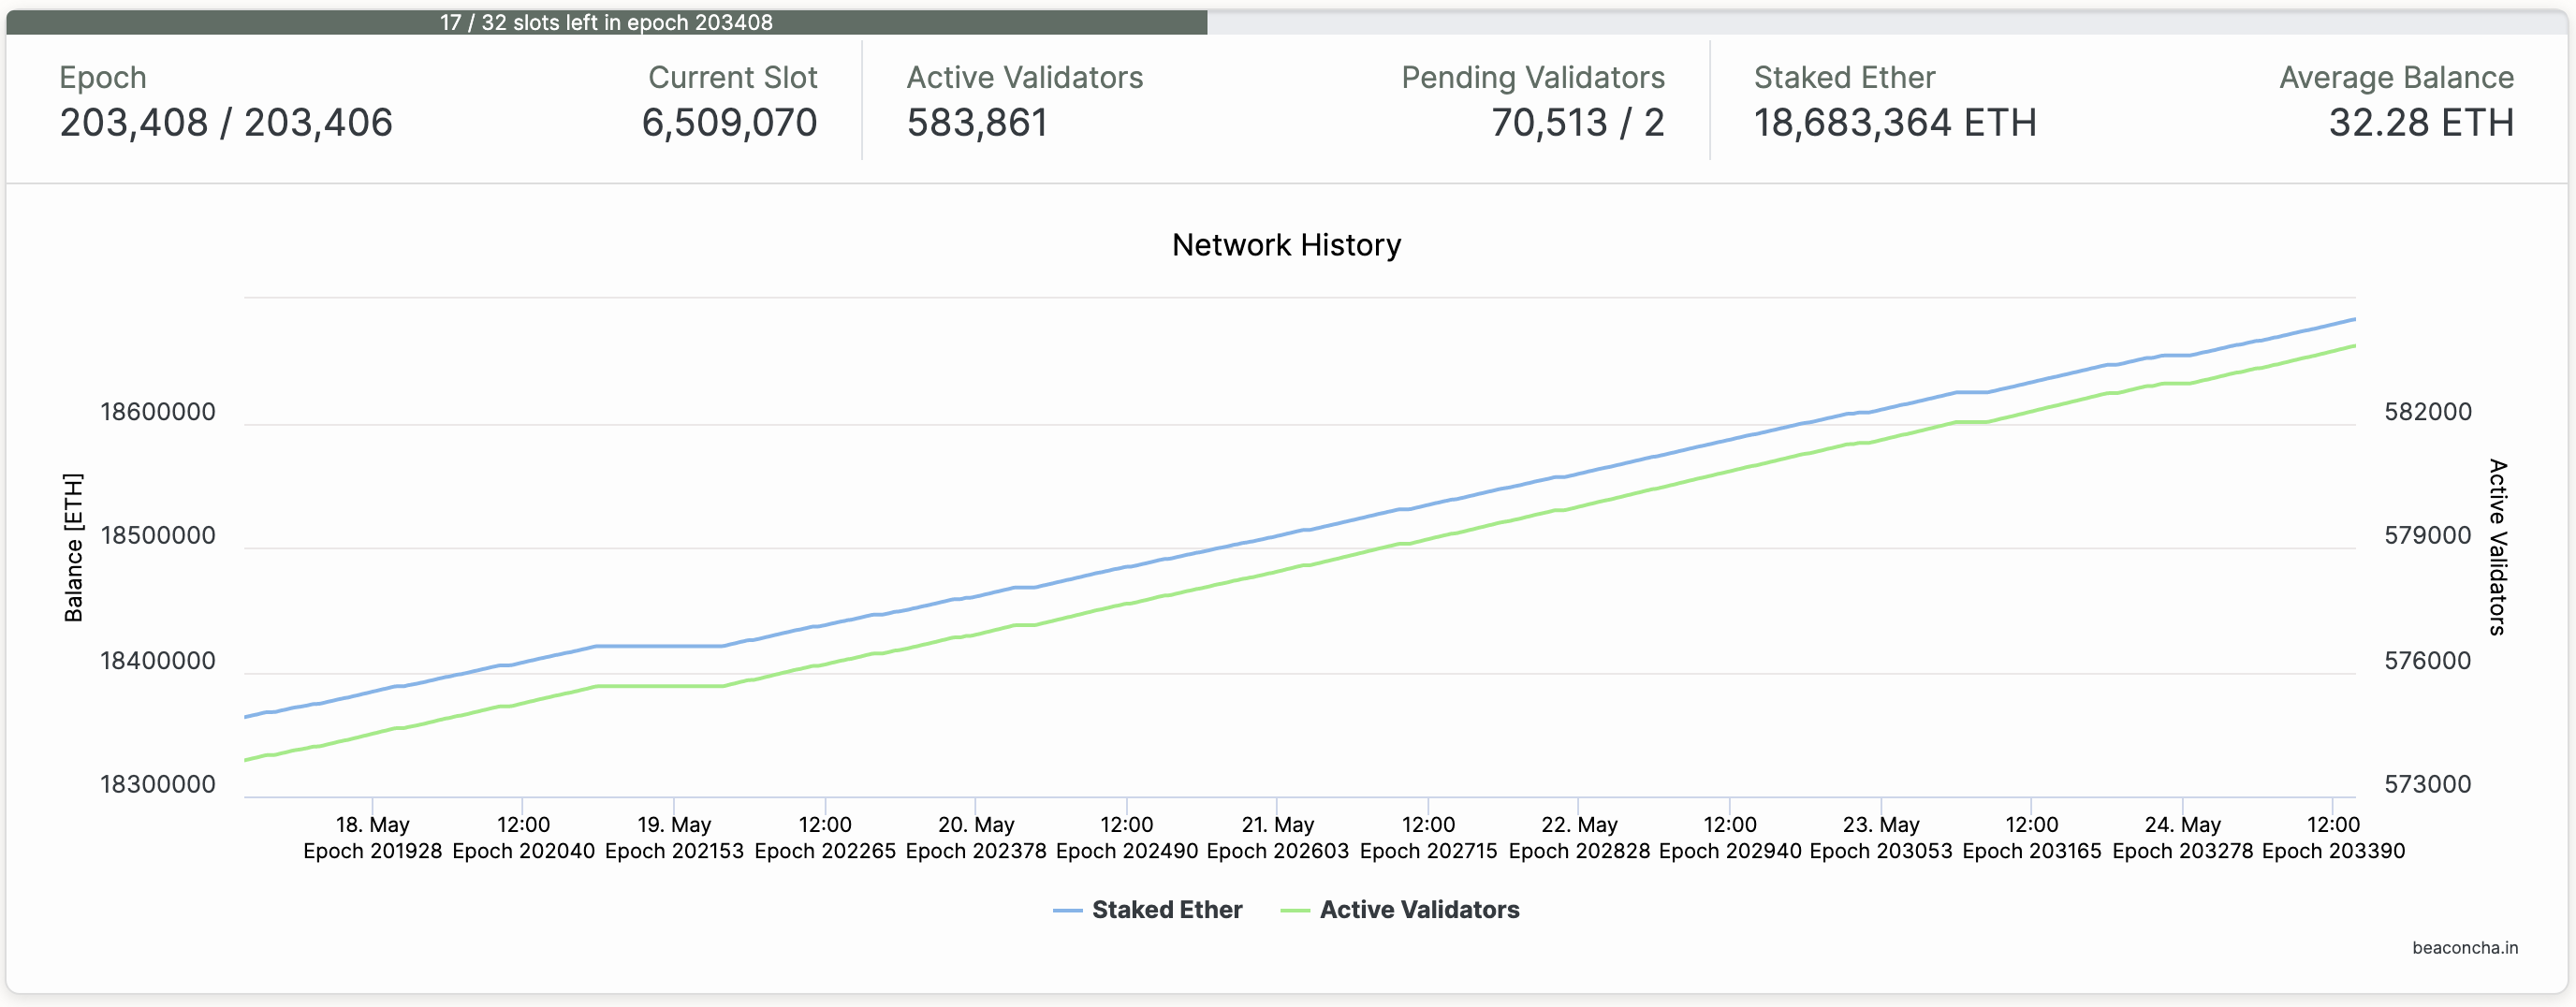
\includegraphics[width=0.9\linewidth]{images/bhomepg}
\caption{Homepage of beaconcha.in showing a progress line of the slots in the current epoch with a graph of total staked Ether and active validators over the last week, from Beaconcha.in (24 May 2023)}
\label{fig:bhomepg}
\end{center}
\end{figure}

\begin{figure}[htbp]
\begin{center}
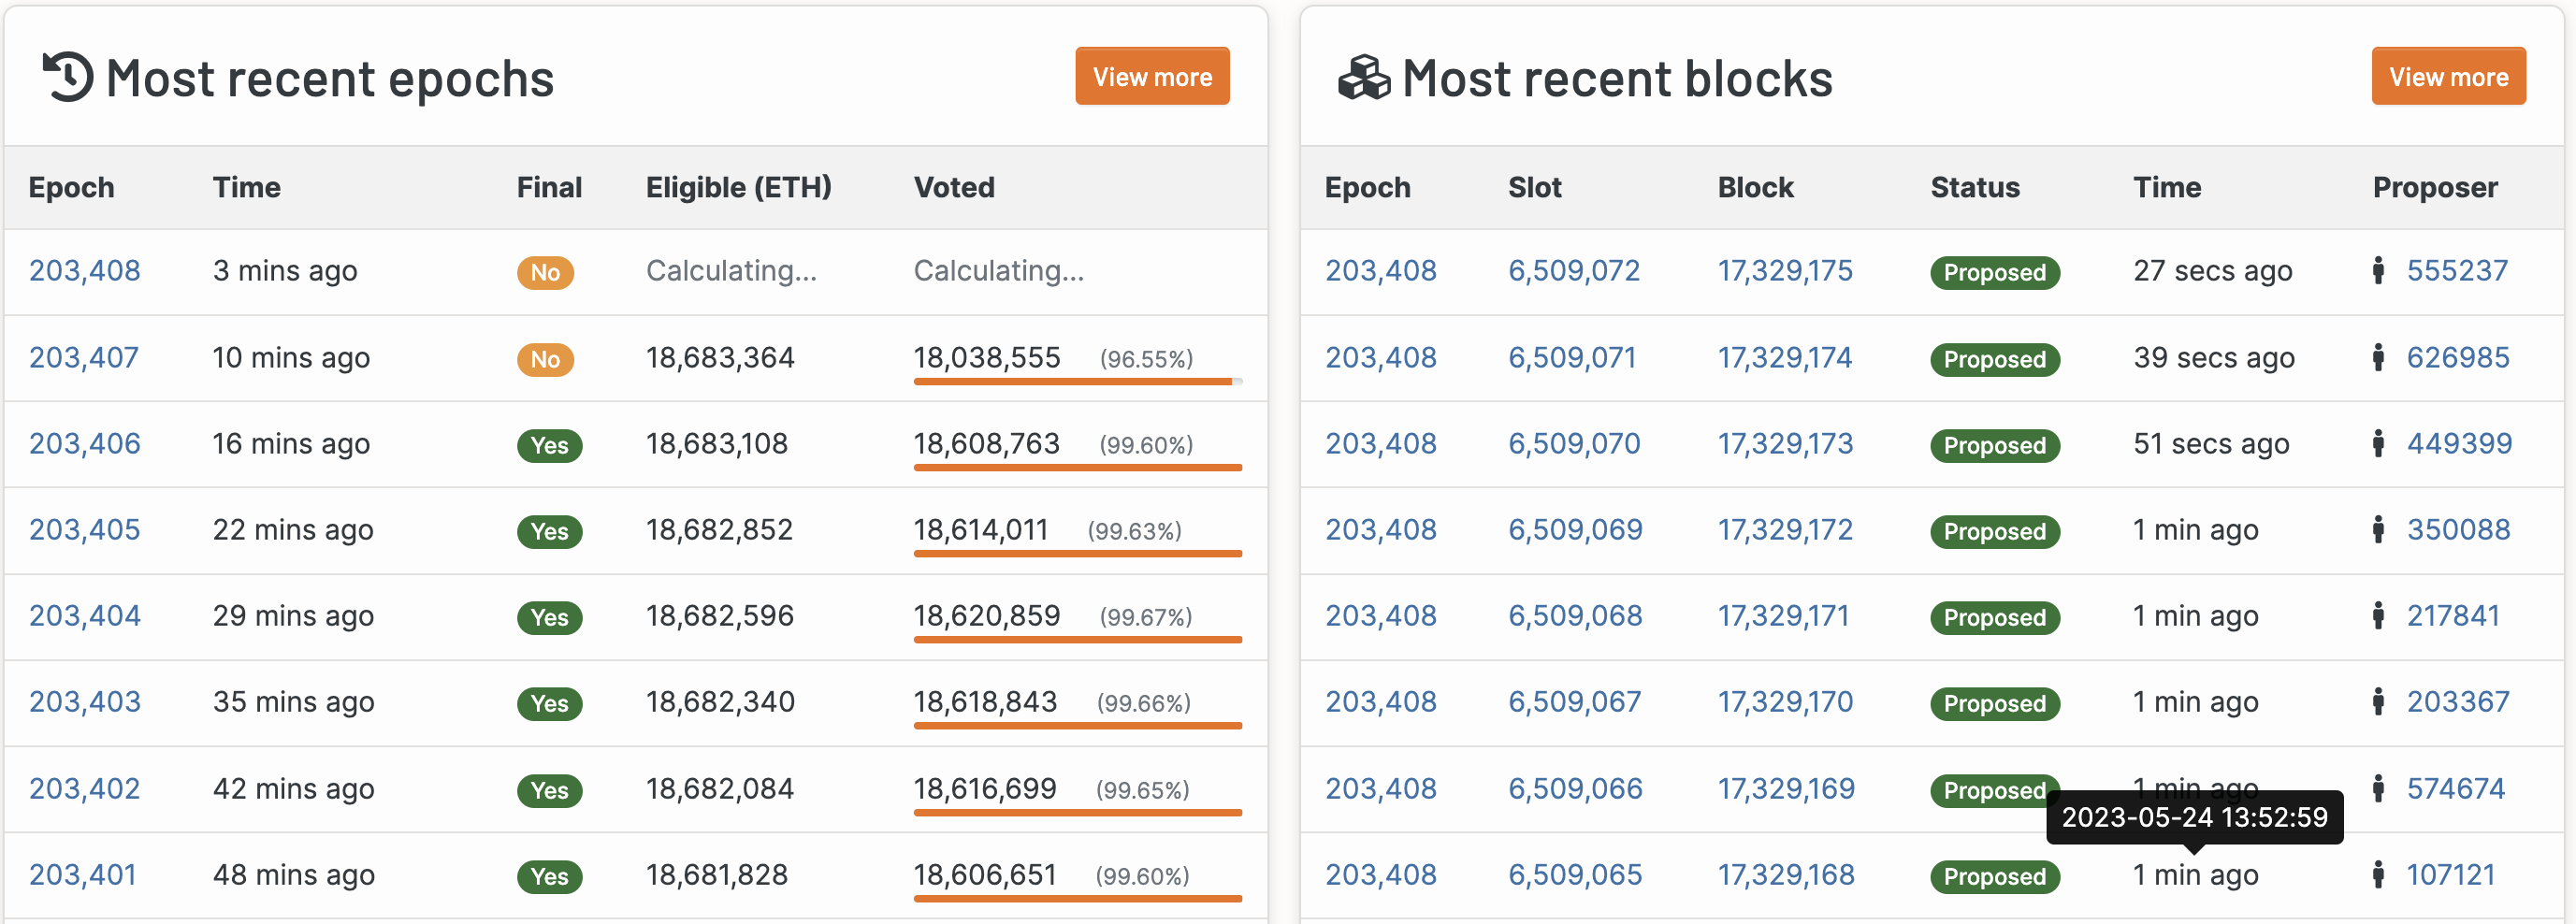
\includegraphics[width=0.9\linewidth]{images/bhomepg2}
\caption{Homepage of beaconcha.in showing the most recent epochs and blocks, from Beaconcha.in (24 May 2023)}
\label{fig:bhomepg2}
\end{center}
\end{figure}
\clearpage


\textbf{Blockchain data}
% -----------------------------
\begin{figure}[htbp]
\begin{center}
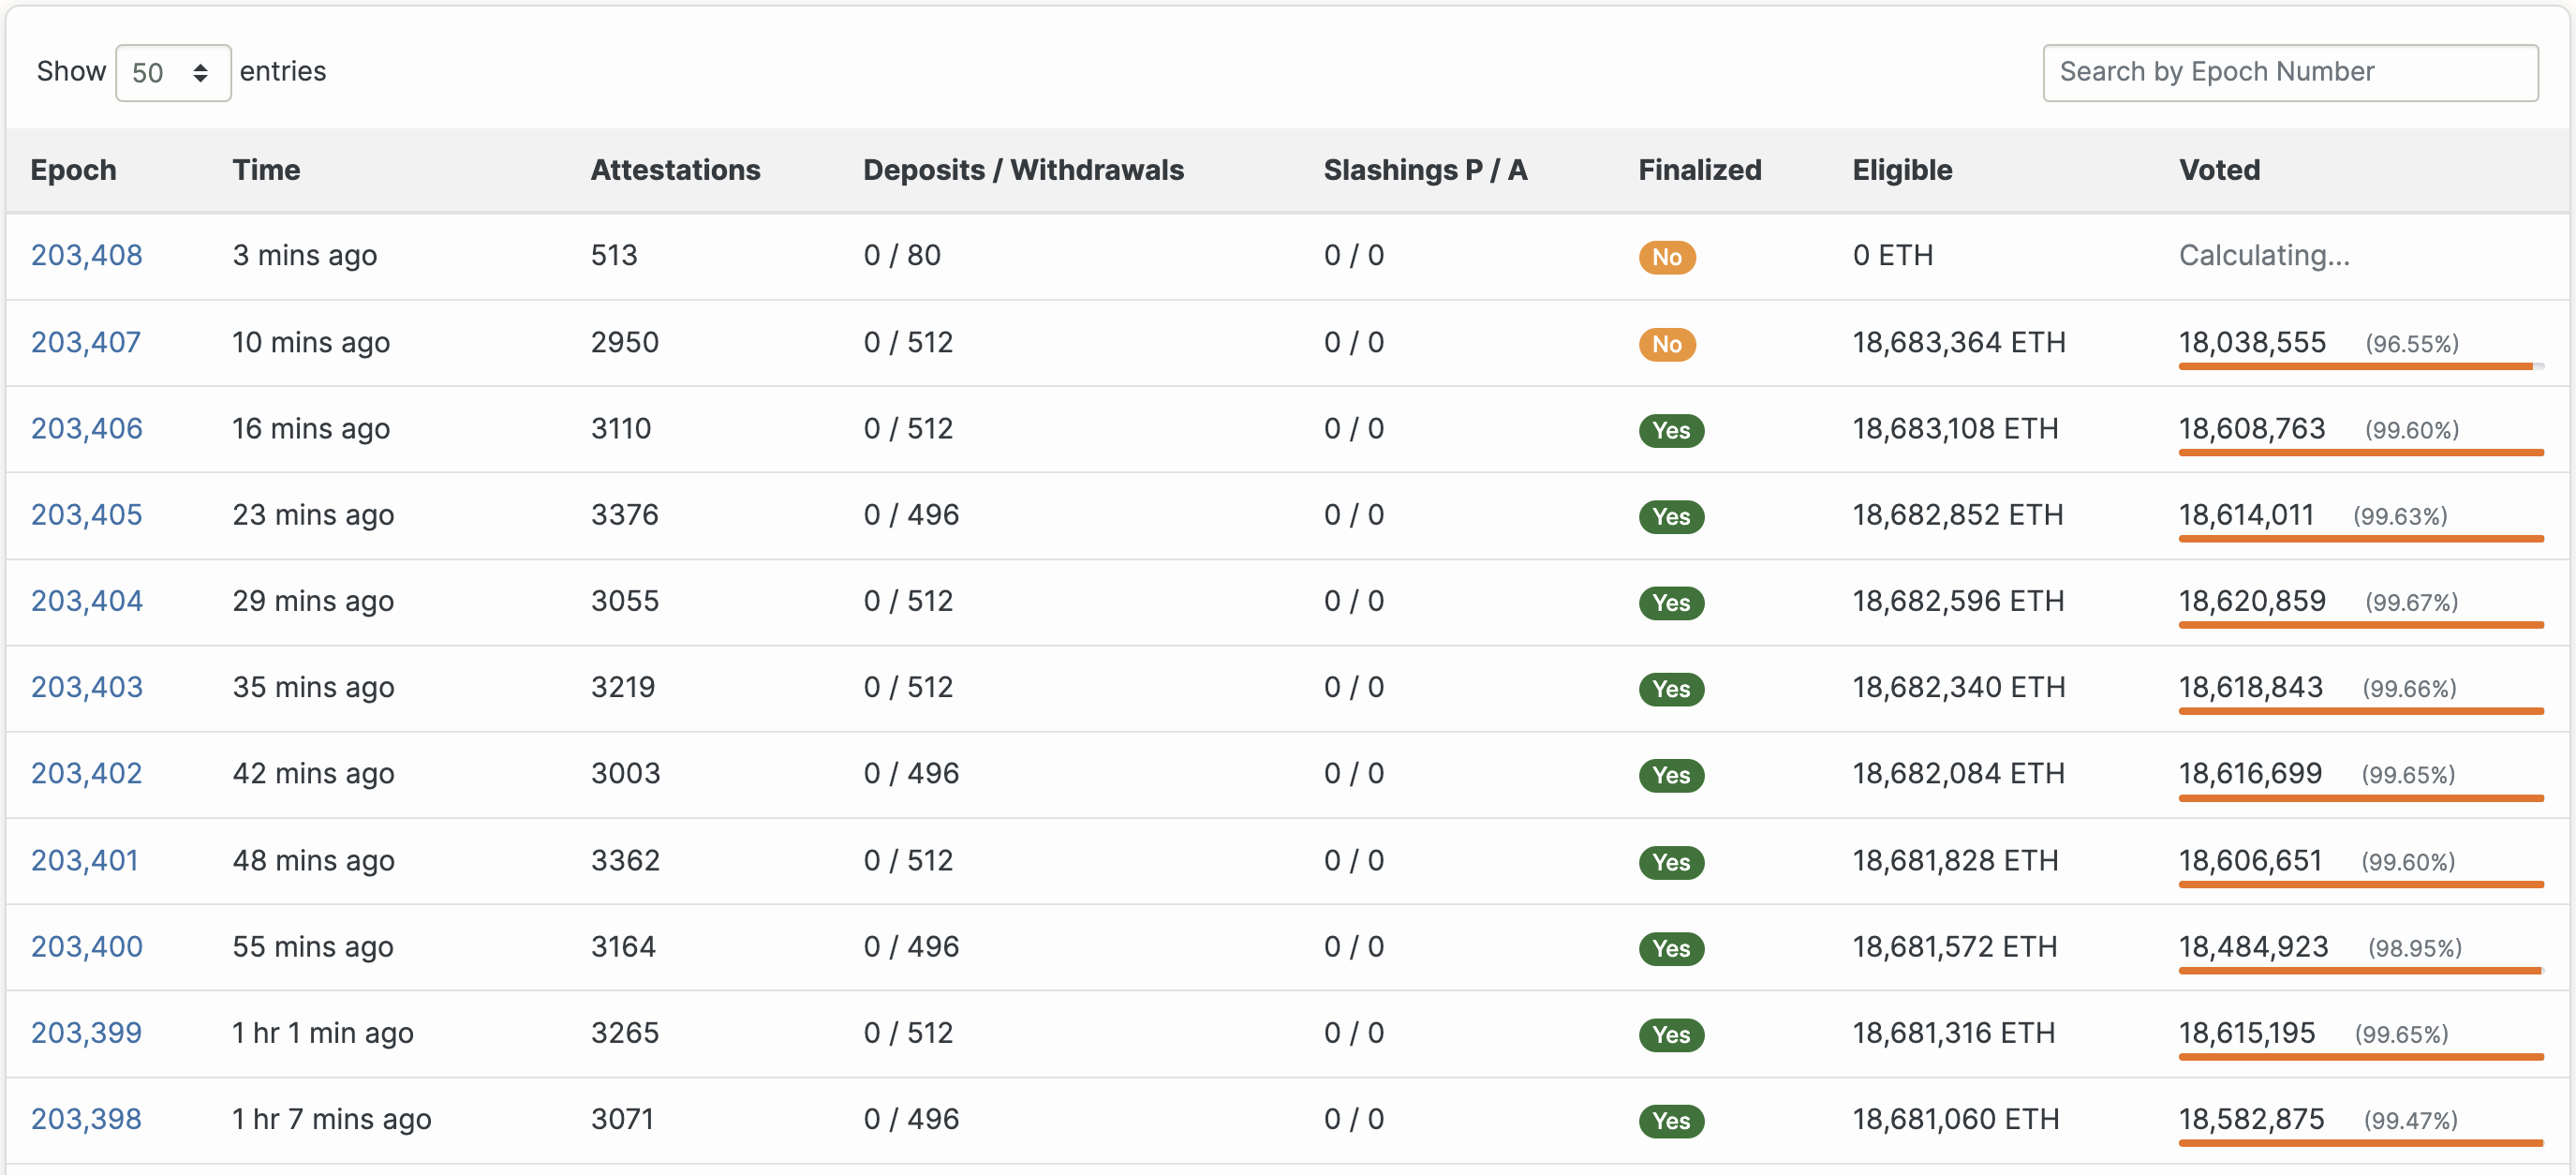
\includegraphics[width=0.9\linewidth]{images/bepochs}
\caption{Detailed information for epochs with the ability to search for a specific epoch, from Beaconcha.in (24 May 2023)}
\label{fig:bepochs}
\end{center}
\end{figure}

\begin{figure}[htbp]
\begin{center}
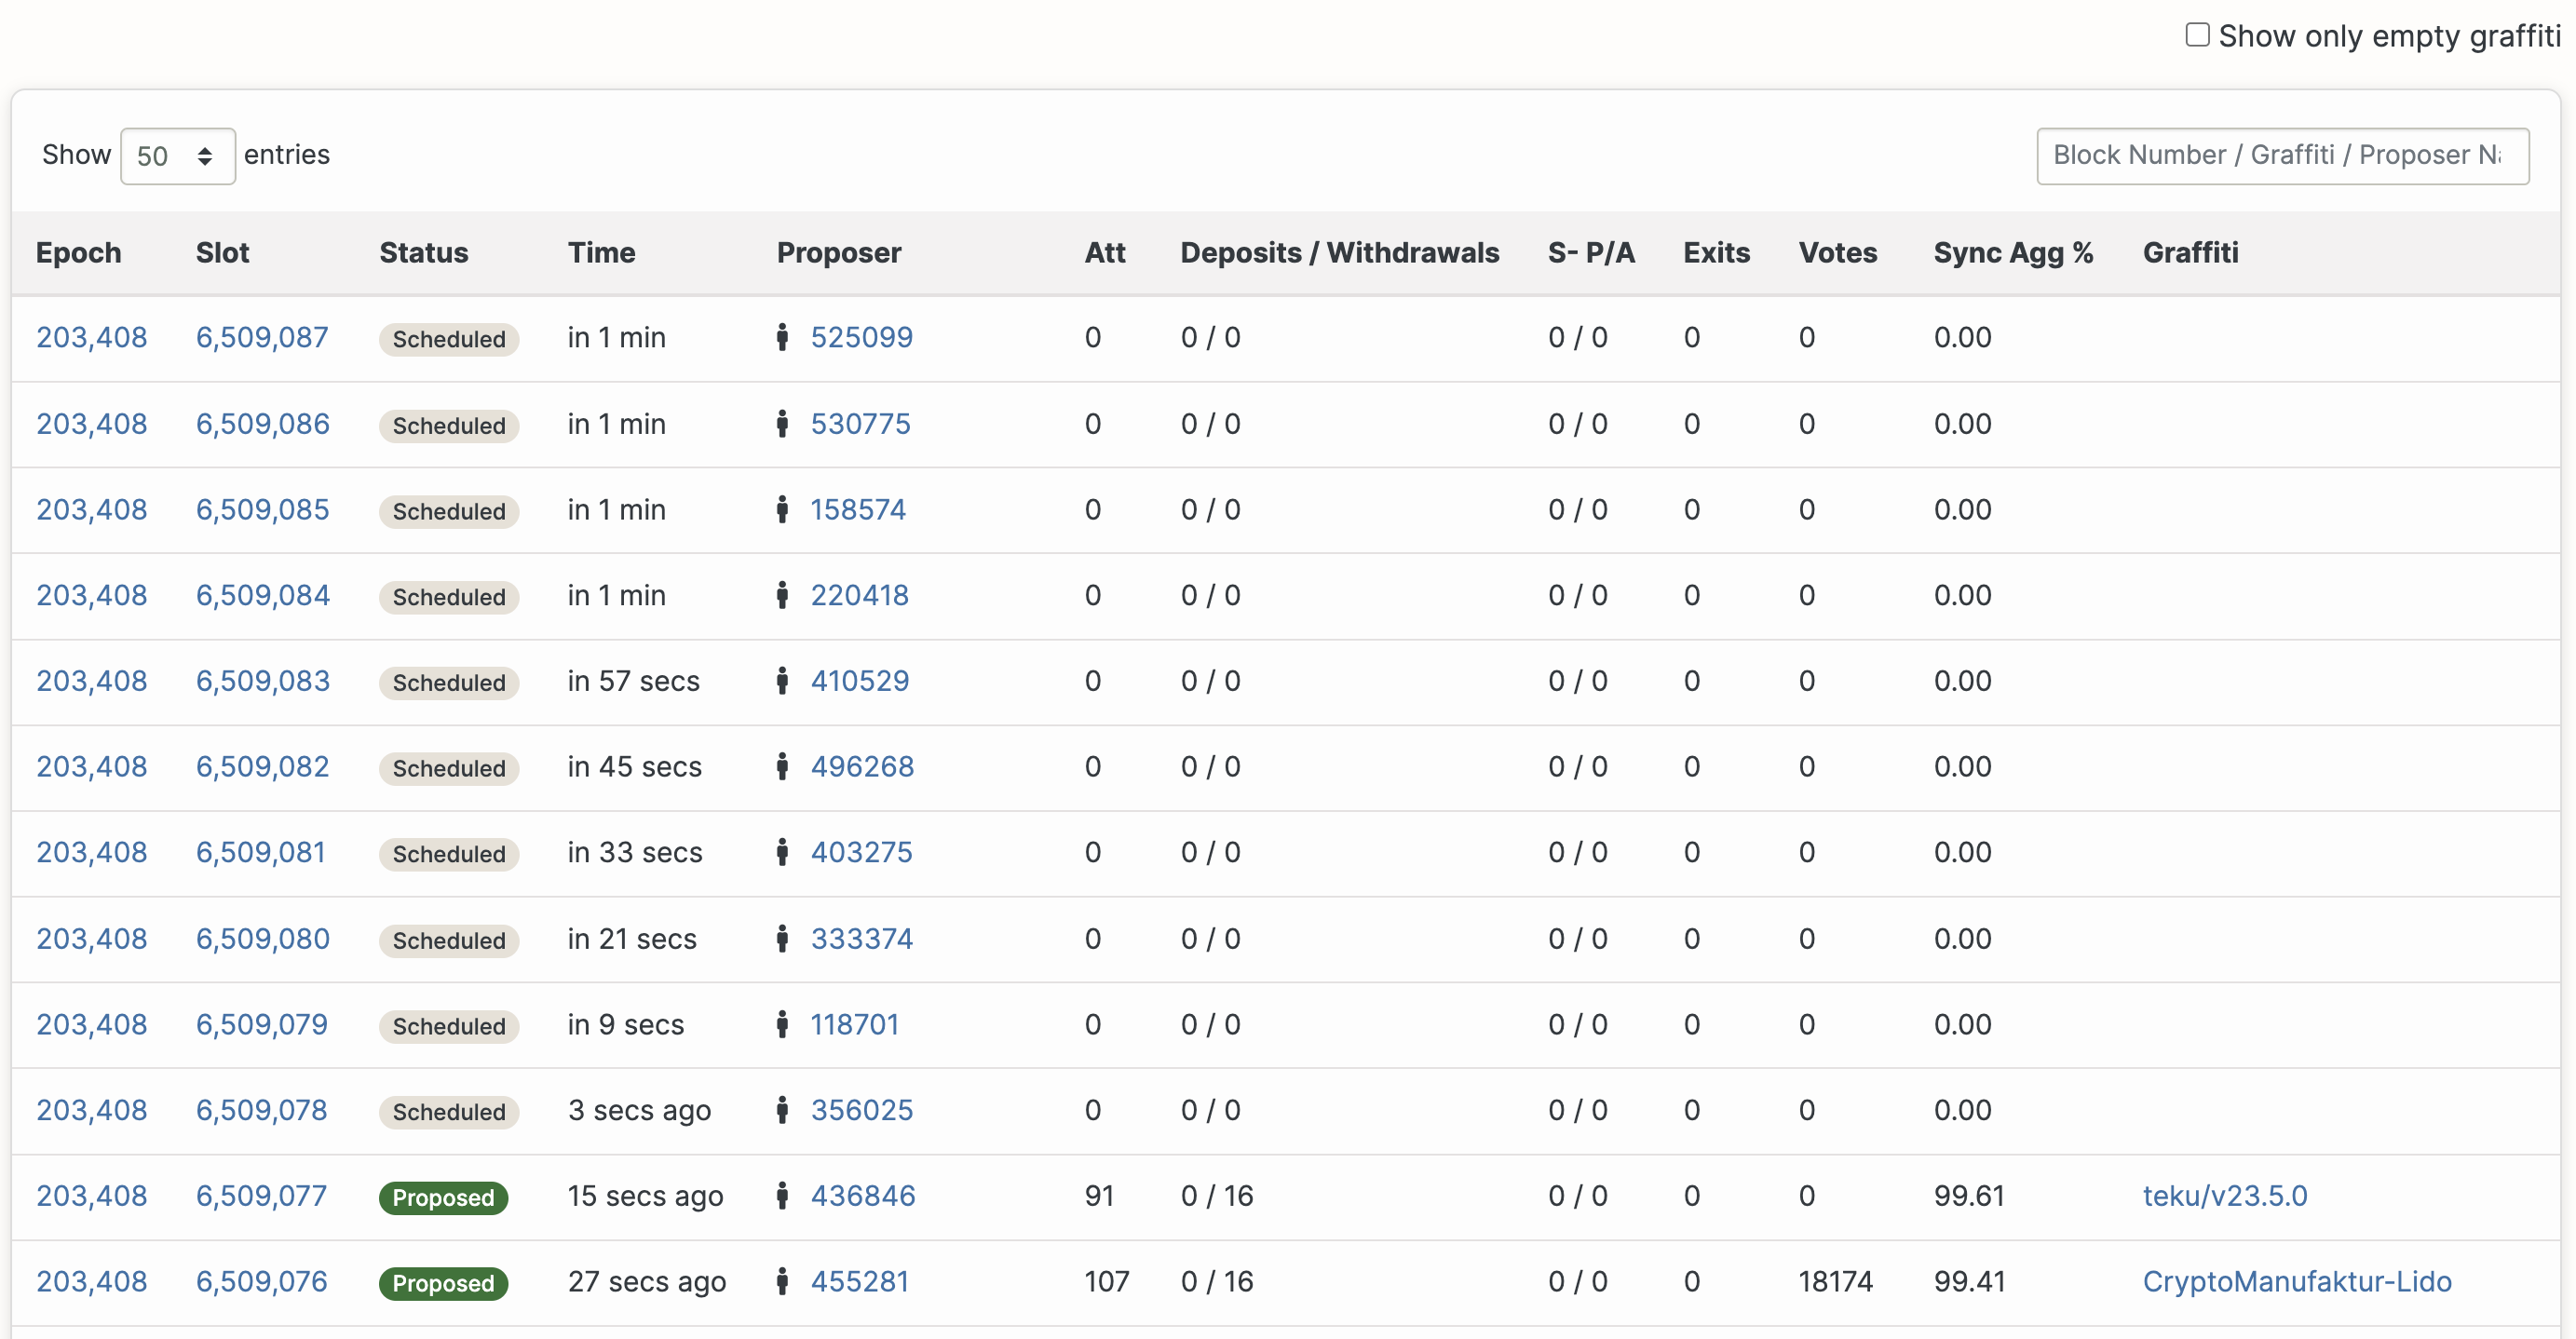
\includegraphics[width=0.9\linewidth]{images/bslots}
\caption{Detailed information for slots with the ability to search by block number, graffiti or proposer number, from Beaconcha.in (24 May 2023)}
\label{fig:bslots}
\end{center}
\end{figure}

\begin{figure}[htbp]
\begin{center}
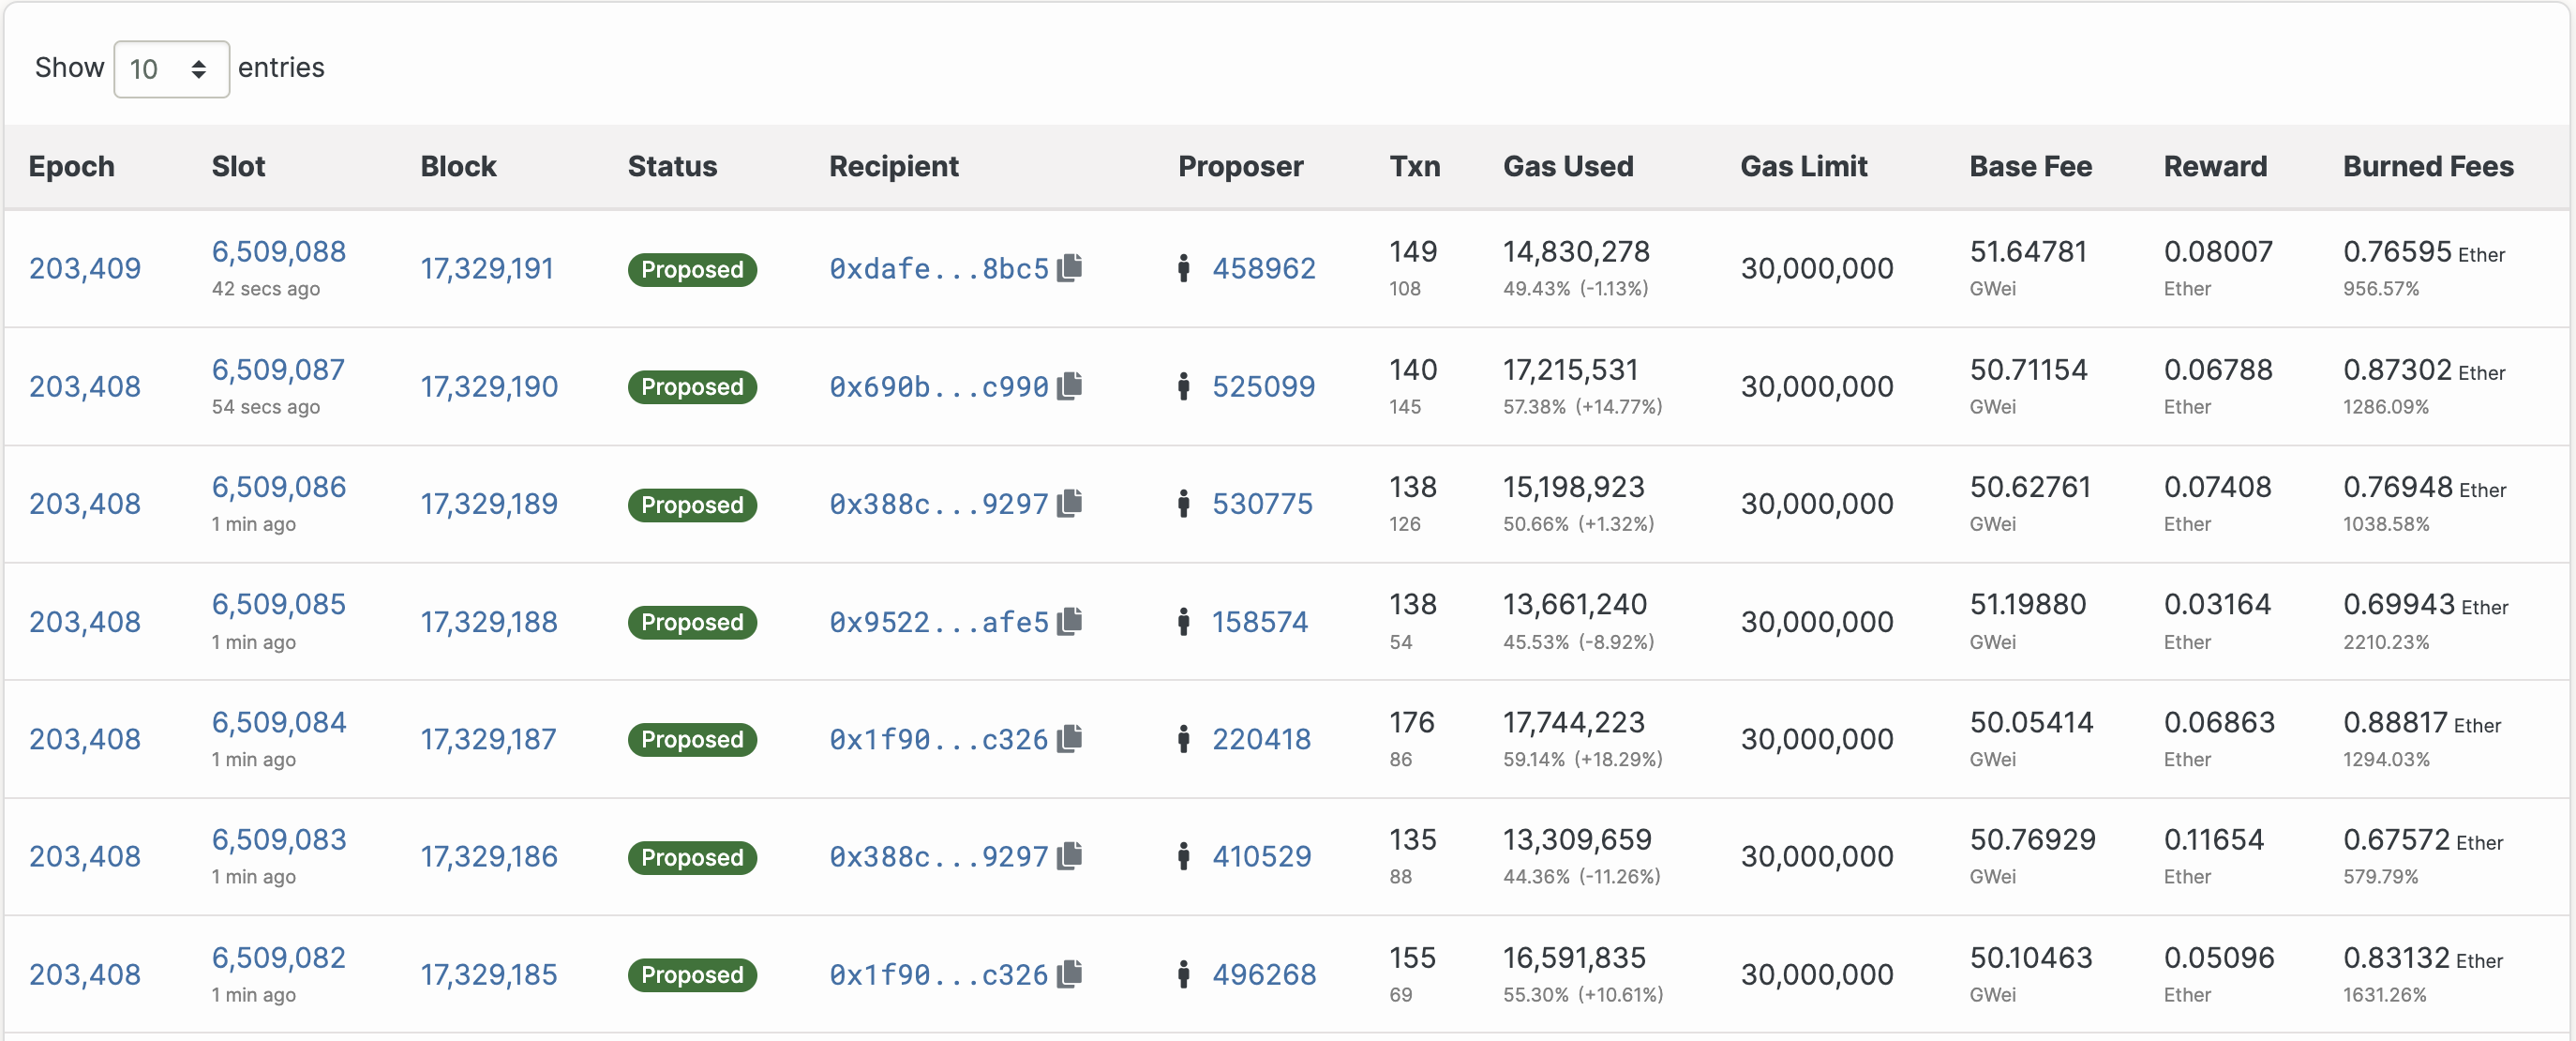
\includegraphics[width=0.9\linewidth]{images/bblocks}
\caption{Detailed information of all blocks, from Beaconcha.in (24 May 2023)}
\label{fig:bblocks}
\end{center}
\end{figure}

\begin{figure}[htbp]
\begin{center}
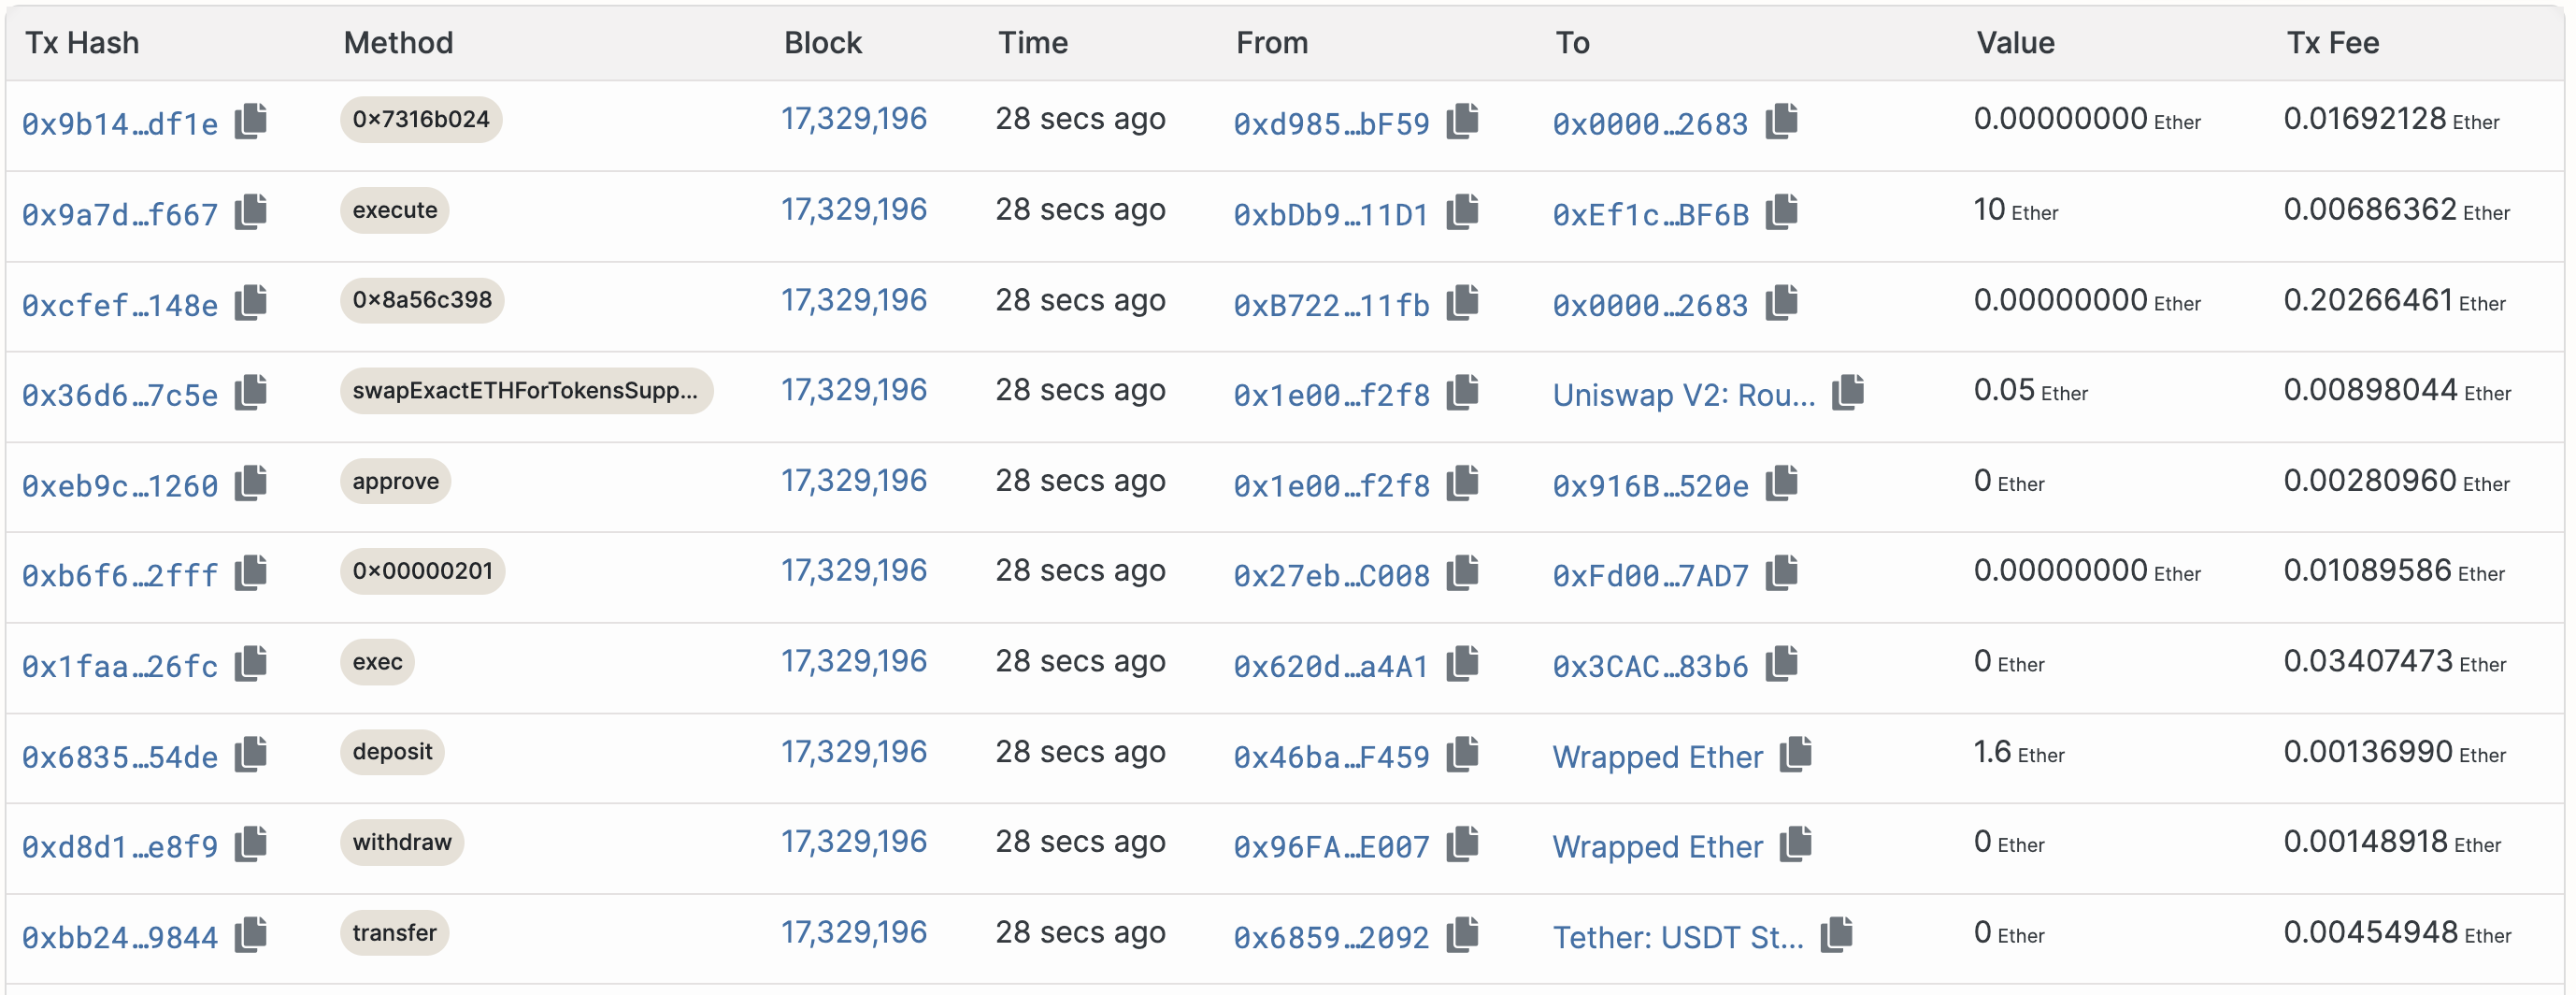
\includegraphics[width=0.9\linewidth]{images/btxns}
\caption{Detailed information of all transactions, from Beaconcha.in (24 May 2023)}
\label{fig:btxns}
\end{center}
\end{figure}

\begin{figure}[htbp]
\begin{center}
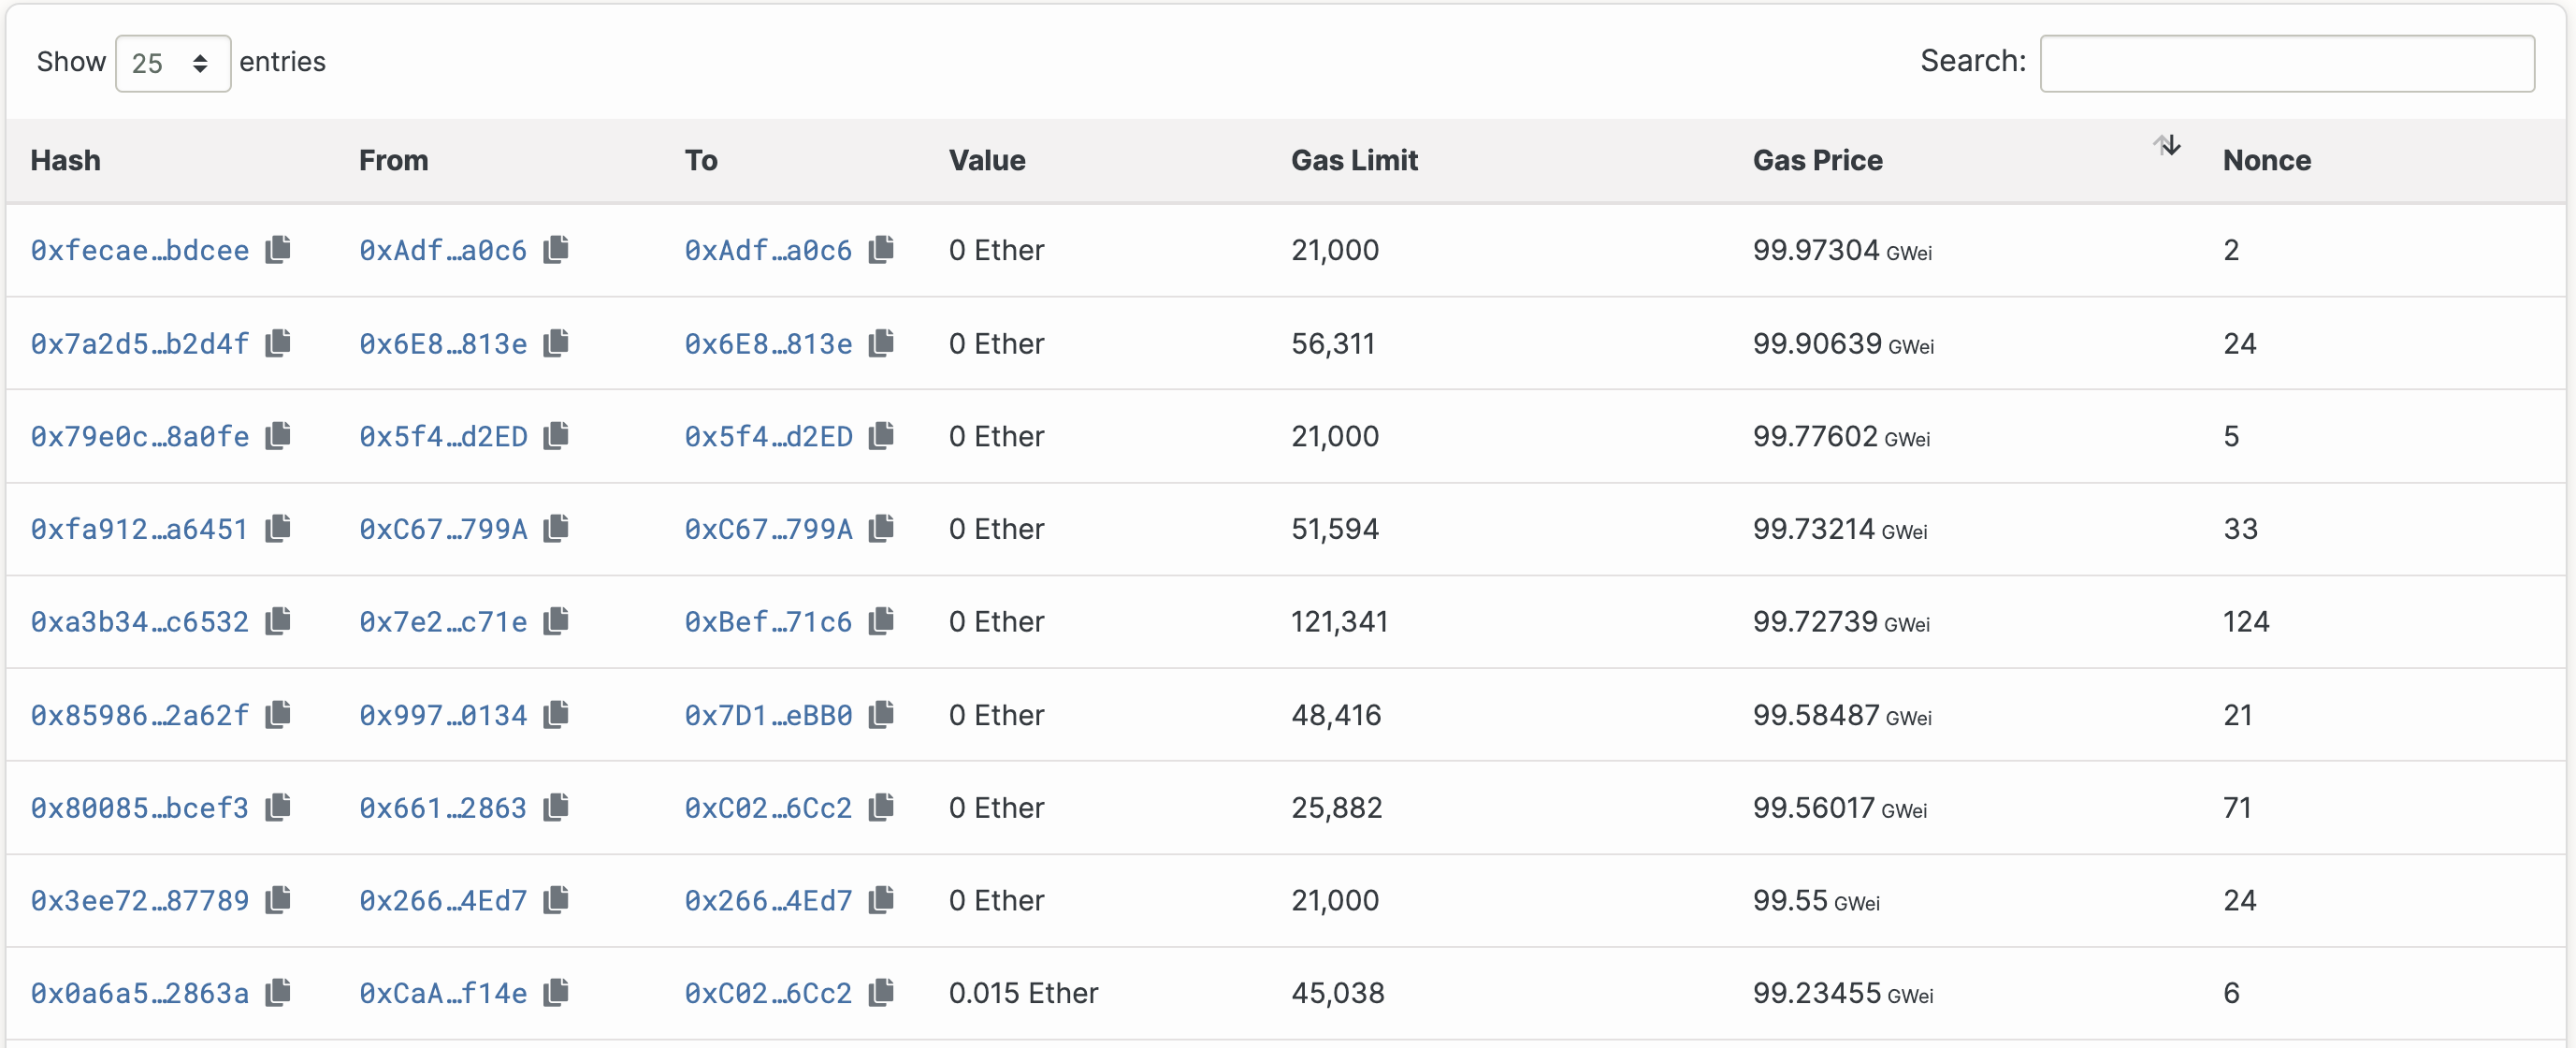
\includegraphics[width=0.9\linewidth]{images/bmempool}
\caption{Mempool transaction details, from Beaconcha.in (24 May 2023)}
\label{fig:bmempool}
\end{center}
\end{figure}
\clearpage


\textbf{Validator data}
% -------------------------
\begin{figure}[htbp]
\begin{center}
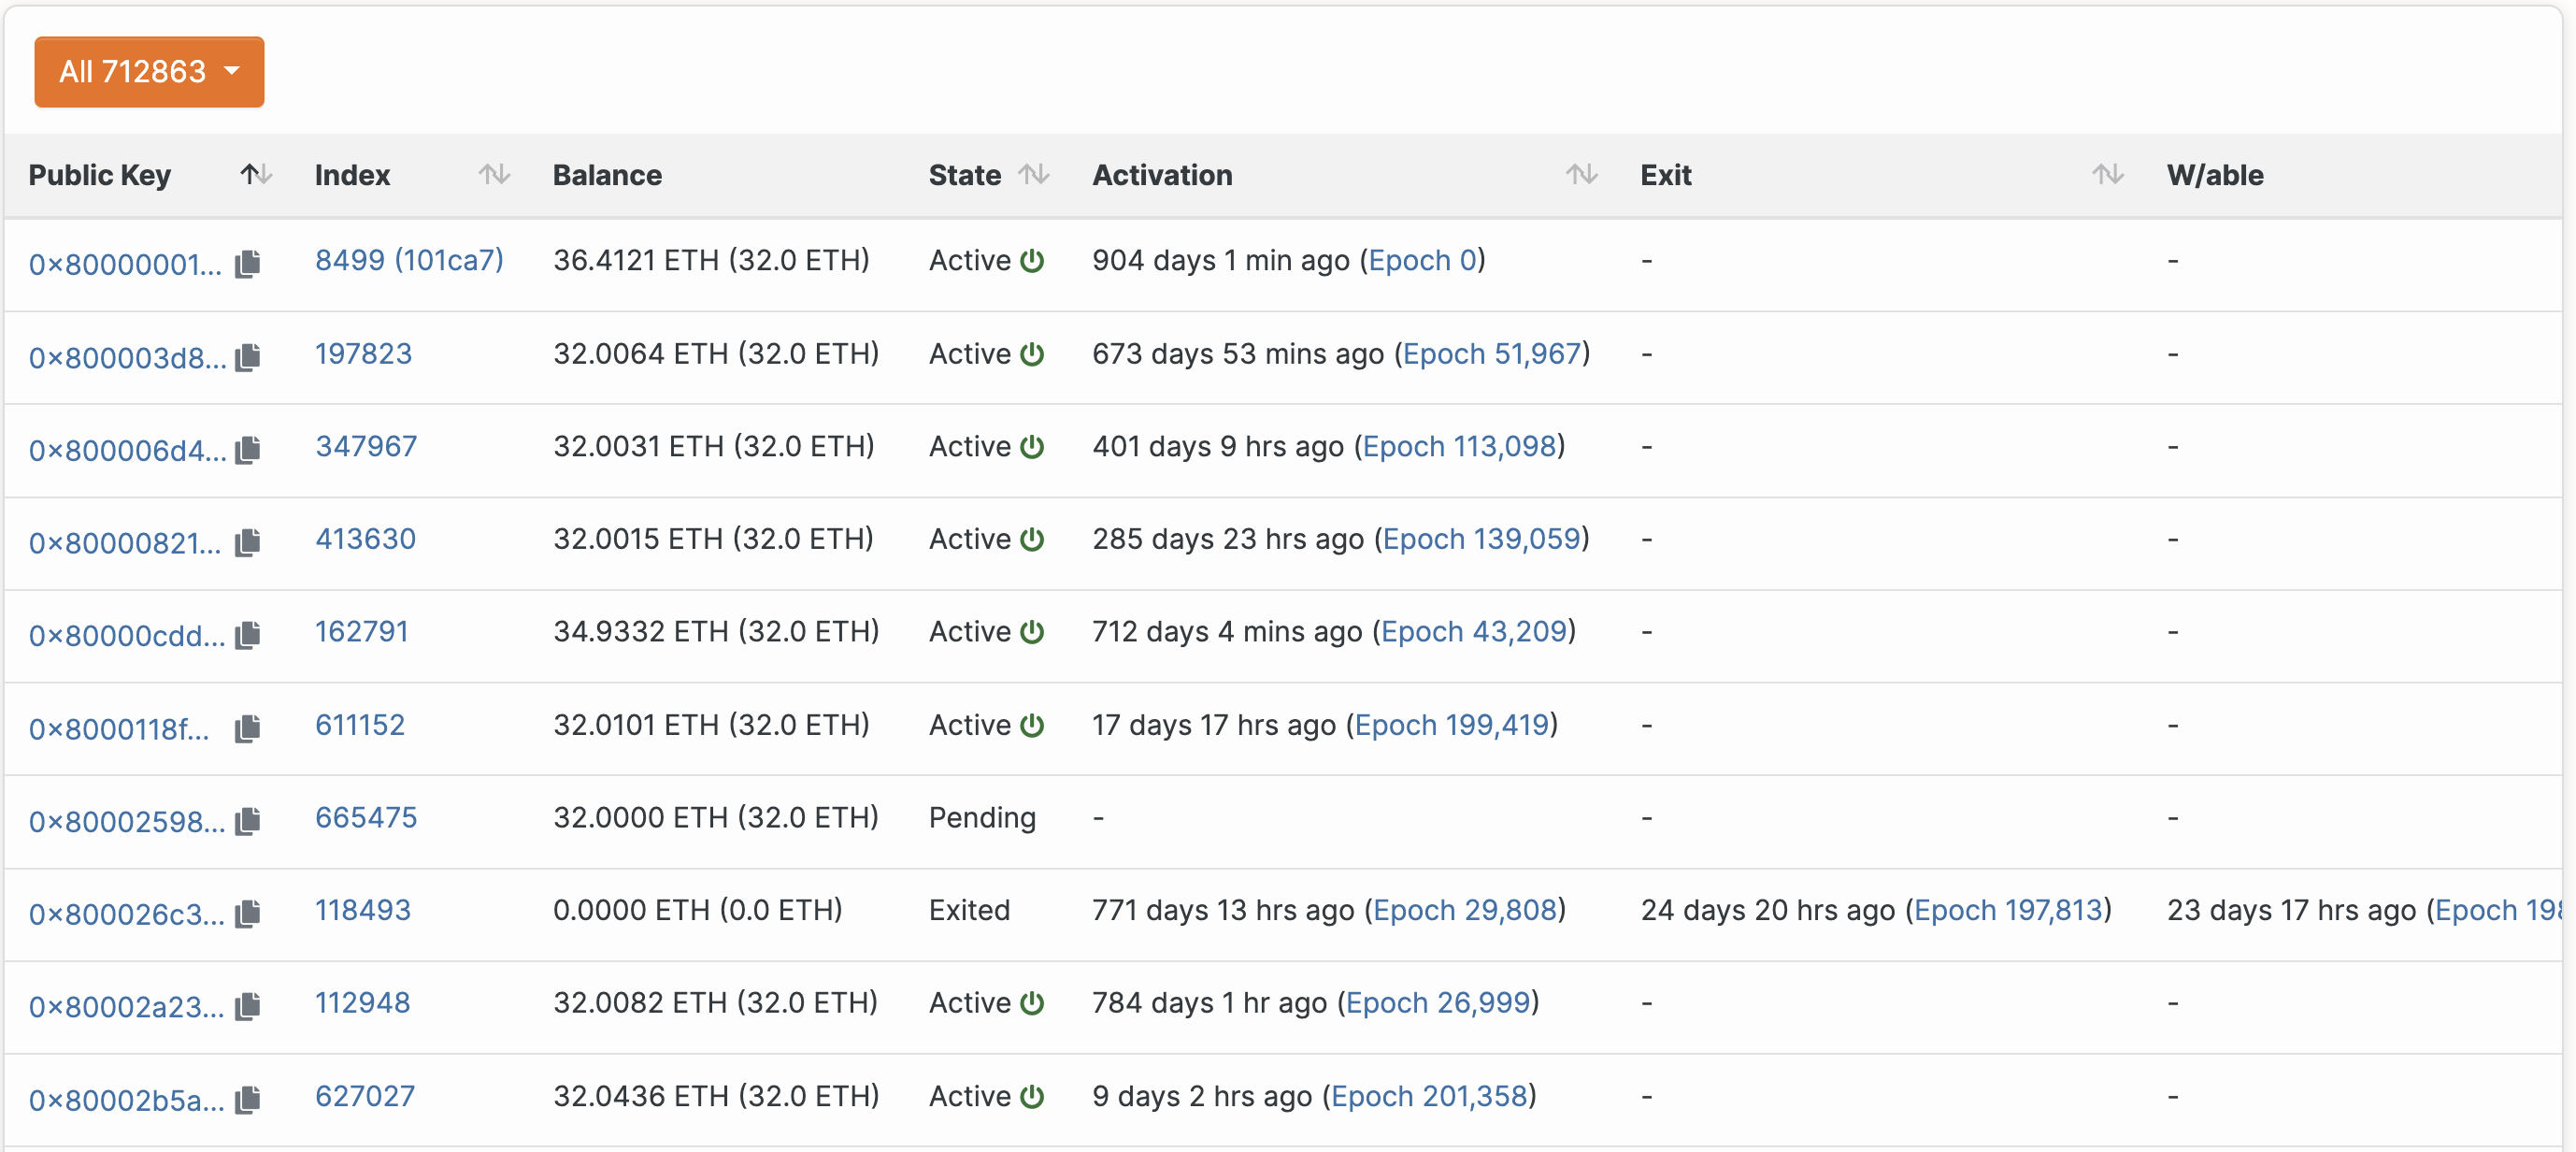
\includegraphics[width=0.9\linewidth]{images/bvalidators}
\caption{Overview of validators. Beaconcha.in (24 May 2023)}
\label{fig:bvalidators}
\end{center}
\end{figure}

\begin{figure}[htbp]
\begin{center}
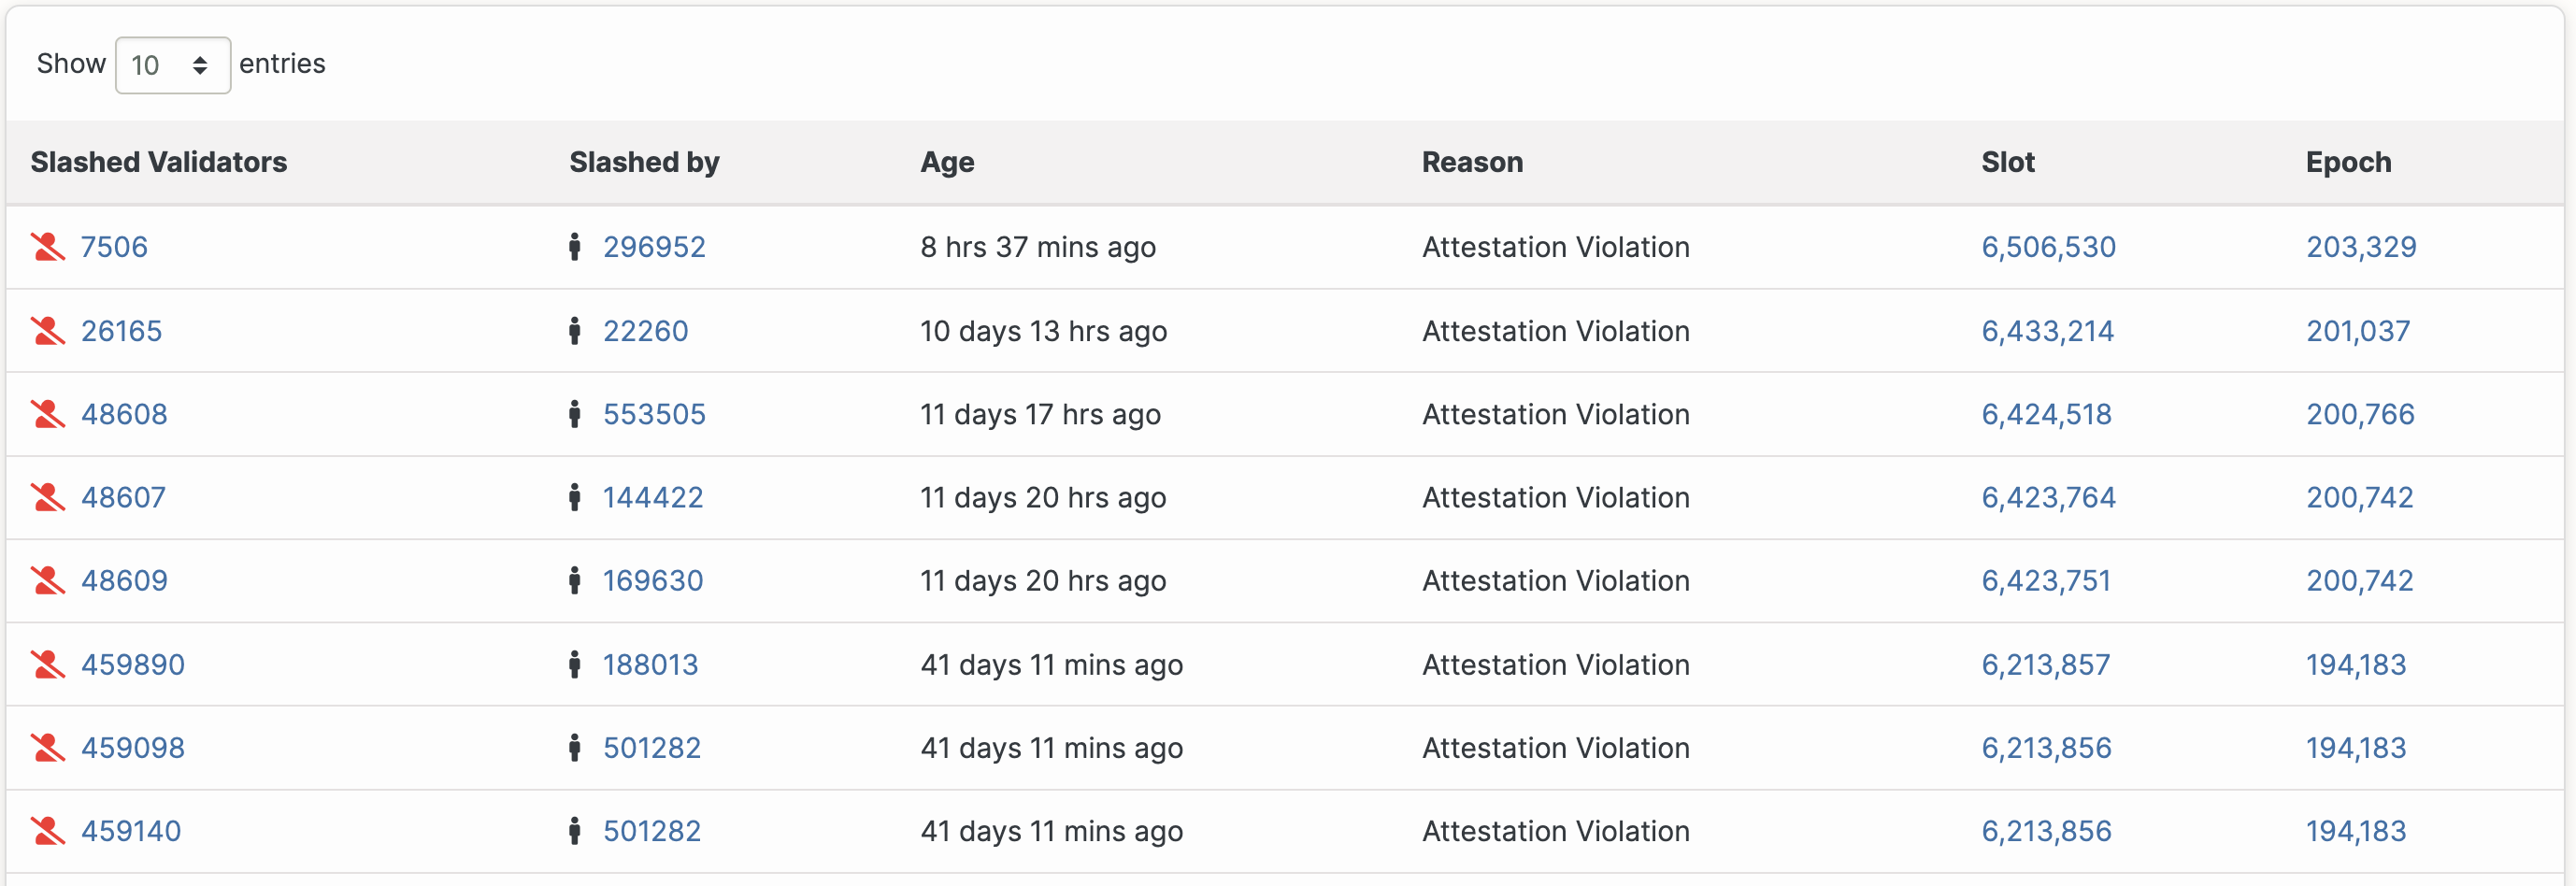
\includegraphics[width=0.9\linewidth]{images/bslashed}
\caption{Slahed validators. Beaconcha.in (24 May 2023)}
\label{fig:bslashed}
\end{center}
\end{figure}

\begin{figure}[htbp]
\begin{center}
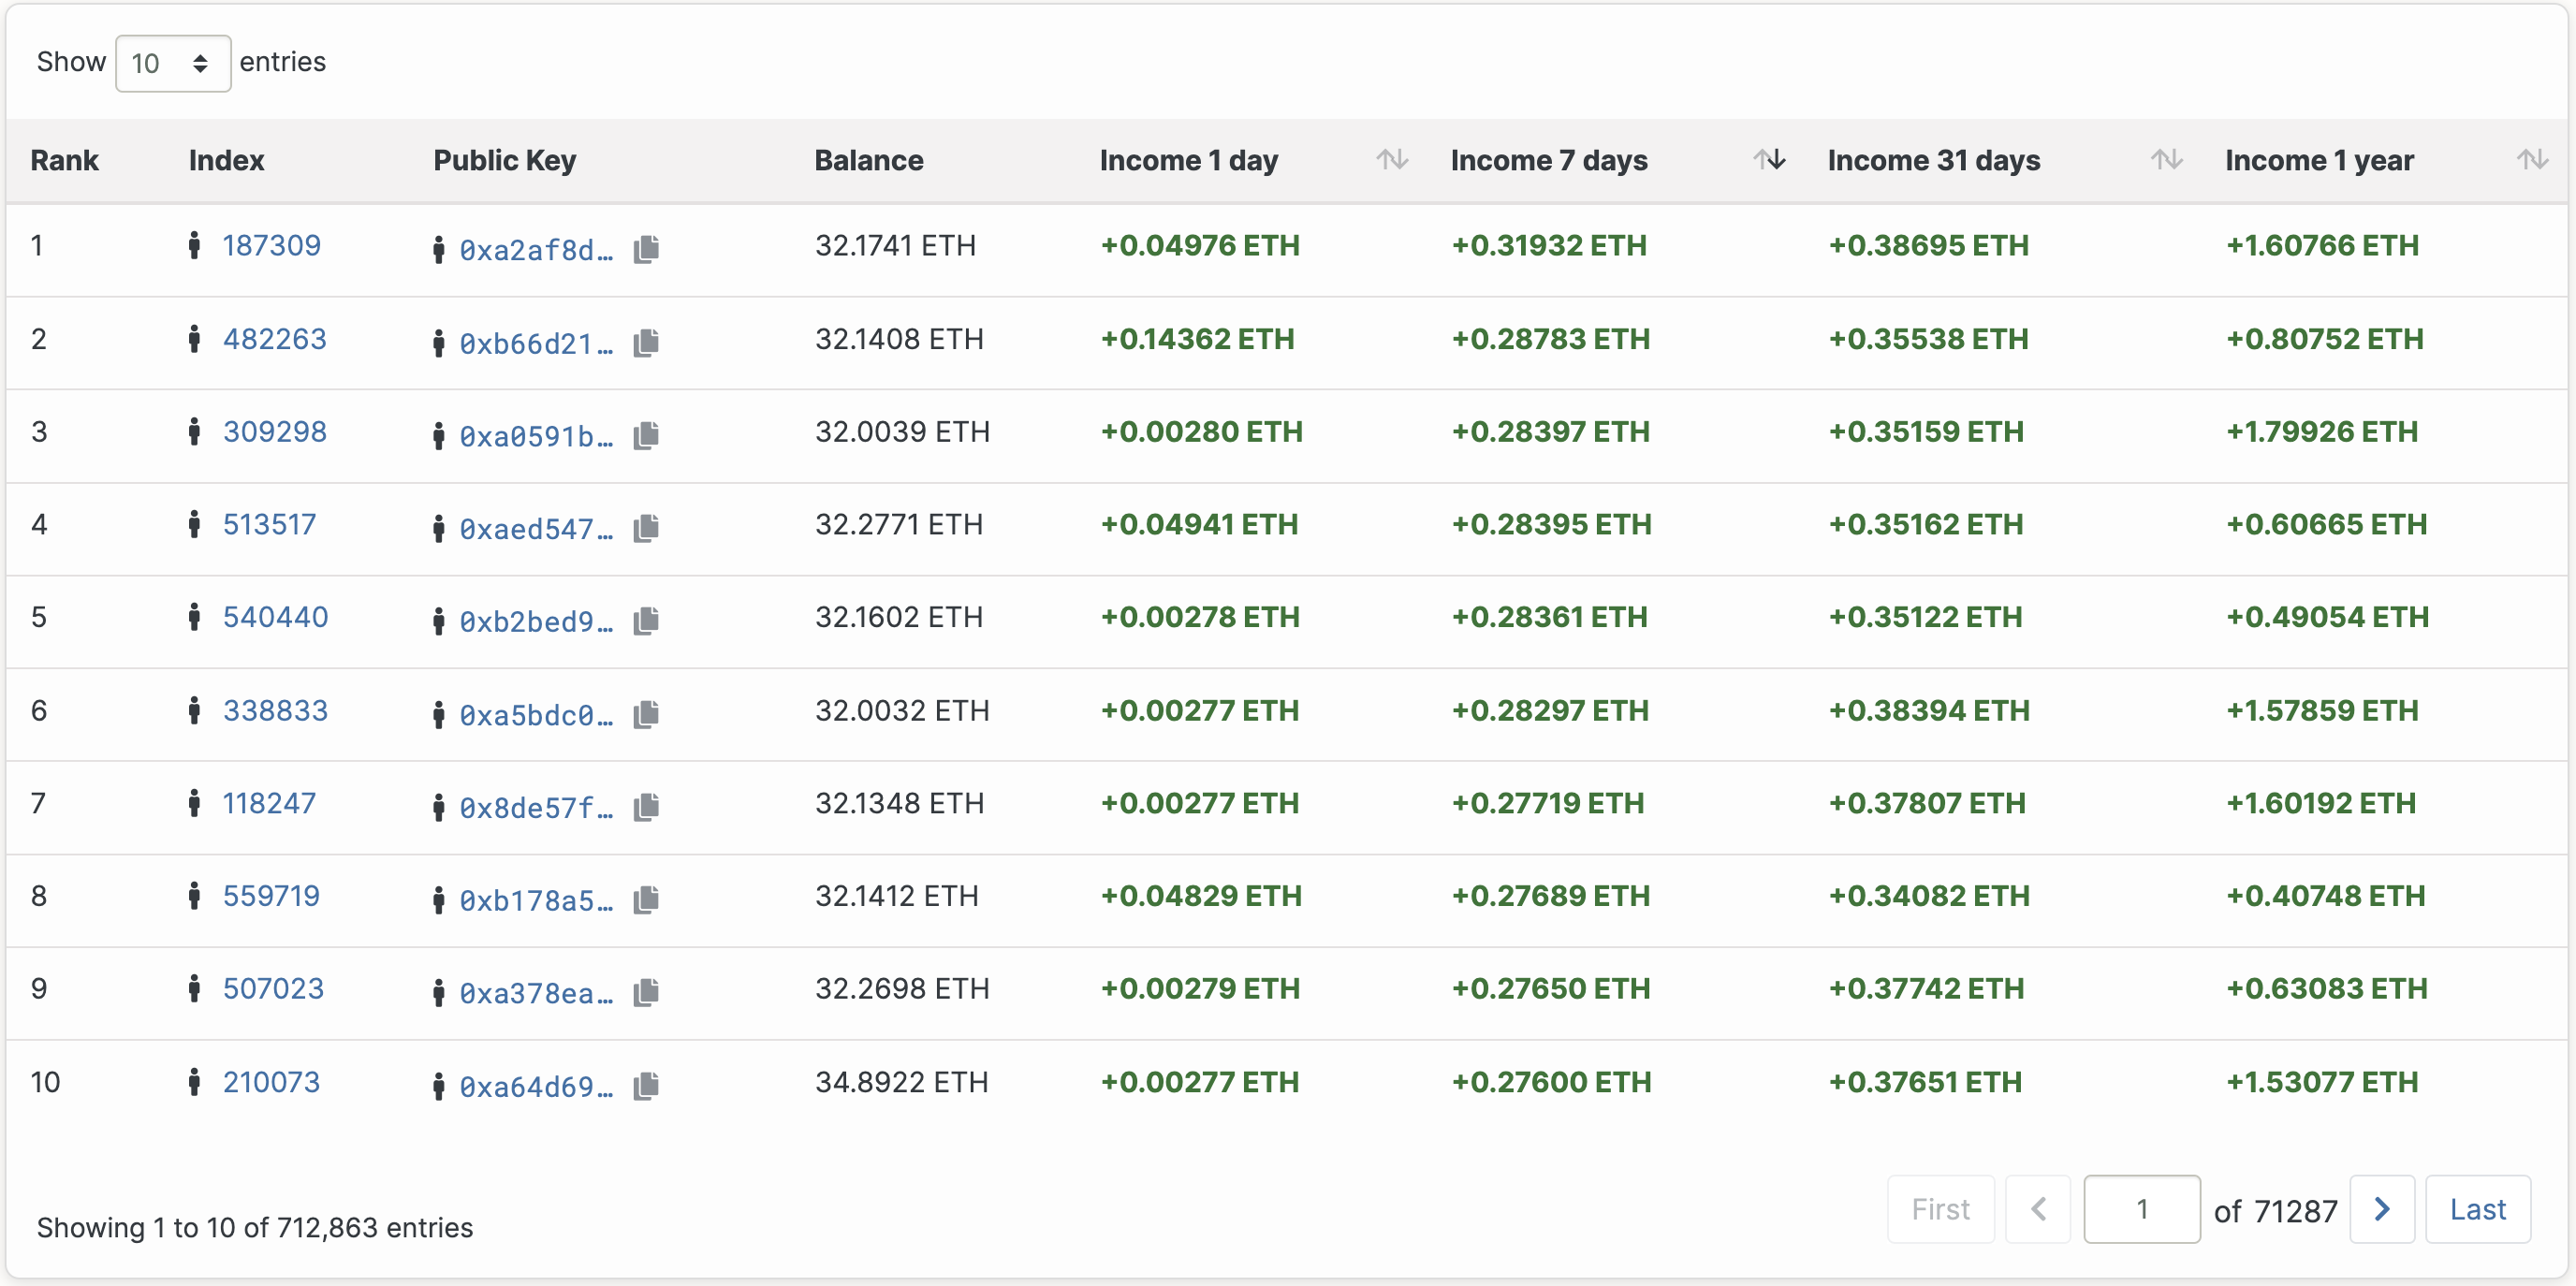
\includegraphics[width=0.9\linewidth]{images/bvalleader}
\caption{Validator leaderboard - default listing order is by 7day income, but it is possible to display the order by income based on 1day, 31 days or 1 year. Beaconcha.in (24 May 2023)}
\label{fig:bvalleader}
\end{center}
\end{figure}

\begin{figure}[htbp]
\begin{center}
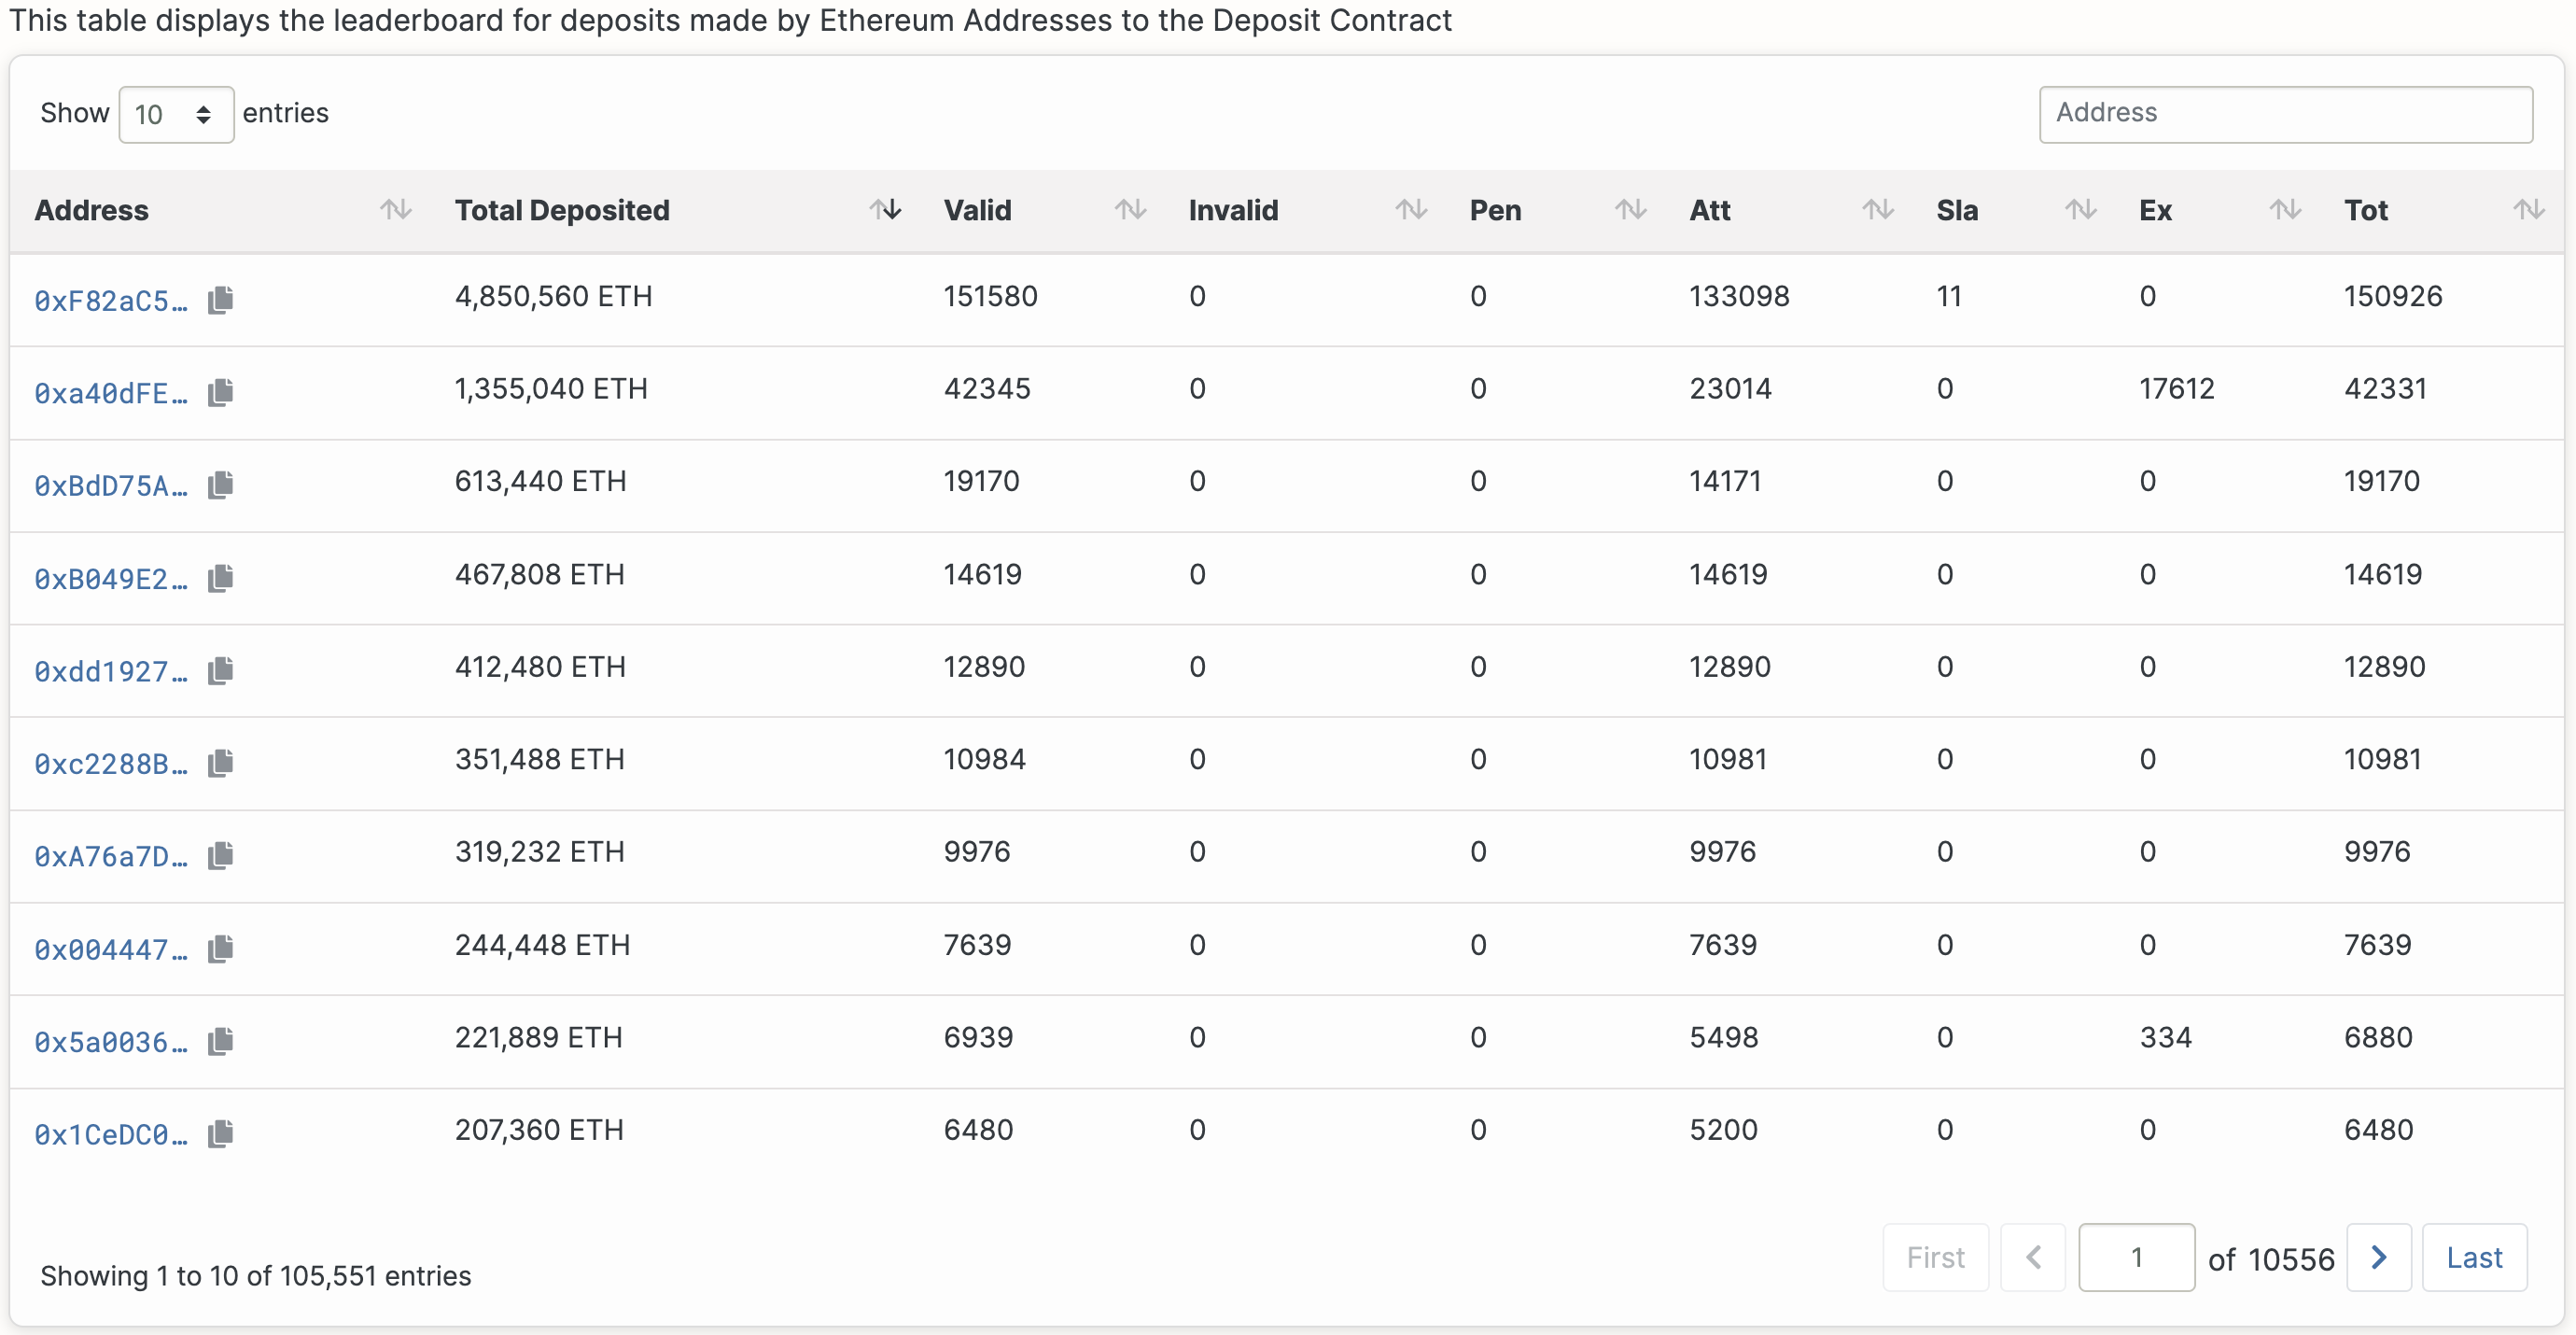
\includegraphics[width=0.9\linewidth]{images/bdepleadtbl}
\caption{Leaderboard for deposits made by Ethereum addresses to the deposit contract - default order is by total amount deposited, but it is possible to display the order using any of the other columns shown in the table. Beaconcha.in (24 May 2023)}
\label{fig:bdepleadtbl}
\end{center}
\end{figure}

\begin{figure}[htbp]
\begin{center}
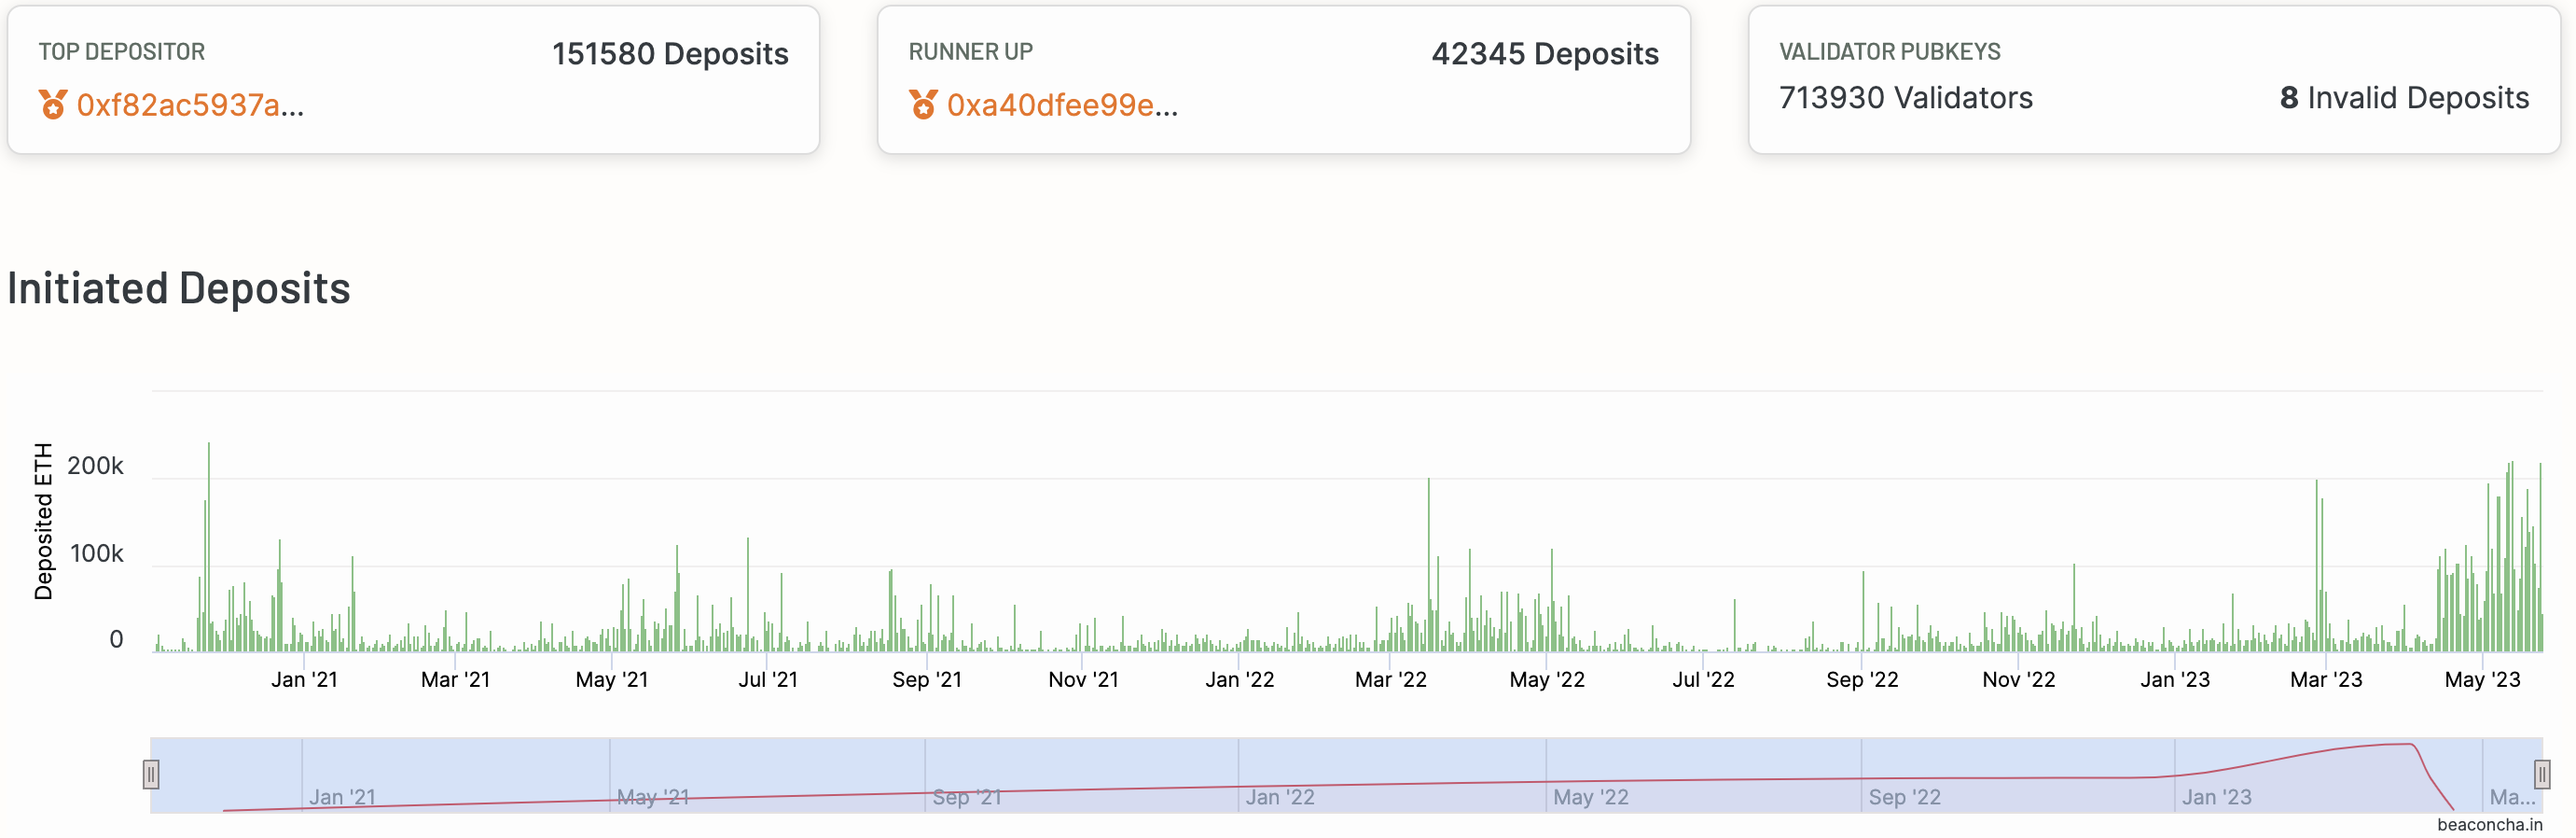
\includegraphics[width=0.9\linewidth]{images/bdeposits}
\caption{Visualisation of deposits since beaconchain genesis. Beaconcha.in (24 May 2023)}
\label{fig:bdeposits}
\end{center}
\end{figure}

\begin{figure}[htbp]
\begin{center}
\includegraphics[width=0.9\linewidth]{images/bdeposittbl}
\caption{Initiated deposits: table of the deposits made by validators wishing to join the beaconchain.. Beaconcha.in (24 May 2023)}
\label{fig:bdeposittbl}
\end{center}
\end{figure}

\begin{figure}[htbp]
\begin{center}
\includegraphics[width=0.48\linewidth]{images/bdeposittbltime}
\includegraphics[width=0.48\linewidth]{images/bdeposittblamount} \\
(a)\hspace{160pt}        (b)\\
\caption{Table of deposits ordered by time (a) and by amount deposited (b). Beaconcha.in (24 May 2023)}
\label{fig:bdeposittbltime}
\end{center}
\end{figure}

\begin{figure}[htbp]
\begin{center}
\includegraphics[width=0.9\linewidth]{images/bincldep}
\caption{Included deposits: table of the deposits received by the beaconchain. Beaconcha.in (24 May 2023)}
\label{fig:bincldep}
\end{center}
\end{figure}

\begin{figure}[htbp]
\begin{center}
\includegraphics[width=0.9\linewidth]{images/bwithdrawals}
\caption{Histogram of processed withdrawals. Beaconcha.in (24 May 2023)}
\label{fig:bwithdrawals}
\end{center}
\end{figure}

\begin{figure}[htbp]
\begin{center}
\includegraphics[width=0.9\linewidth]{images/bwithdrawalstbl}
\caption{Table of partial and full withdrawals. Beaconcha.in (24 May 2023)}
\label{fig:bwithdrawalstbl}
\end{center}
\end{figure}

\begin{figure}[htbp]
\begin{center}
\includegraphics[width=0.9\linewidth]{images/bblschgs}
\caption{Table displaying the BLS address changes from 0x00 credentials to 0x01. Beaconcha.in (24 May 2023)}
\label{fig:bblschgs}
\end{center}
\end{figure}

\begin{figure}[htbp]
\begin{center}
\includegraphics[width=0.9\linewidth]{images/bvaldashboard}
\caption{Validator dashboard - add the validators of interest to the search bar. In this example we added three validators: one active, one voluntary exited and one slashed validator. Beaconcha.in (24 May 2023)}
\label{fig:bvaldashboard}
\end{center}
\end{figure}

\begin{figure}[htbp]
\begin{center}
\includegraphics[width=0.9\linewidth]{images/bcorrelations}
\caption{It is possible to generate correlation visualisations between several variables. Beaconcha.in (24 May 2023)}
\label{fig:bcorrelations}
\end{center}
\end{figure}

\clearpage
\textbf{Consensus Layer Charts}\\
% -------------------------------------------
\begin{figure}[htbp]
\begin{center}
\includegraphics[width=0.48\linewidth]{images/bchart1}
\includegraphics[width=0.48\linewidth]{images/bchart2} \\
(a)\hspace{160pt}        (b)\\
\caption{History of daily blocks proposed (a) and daily active validators (b) from Beaconcha.in (24 May 2023)}
\label{fig:chart1}
\end{center}
\end{figure}

\begin{figure}[htbp]
\begin{center}
\includegraphics[width=0.48\linewidth]{images/bchart3}
\includegraphics[width=0.48\linewidth]{images/bchart4} \\
(a)\hspace{160pt}        (b)\\
\caption{History of daily staked Ether (sum of all effective balances) (a) and average daily validator balance (b) from Beaconcha.in (24 May 2023)}
\label{fig:chart3}
\end{center}
\end{figure}

\begin{figure}[htbp]
\begin{center}
\includegraphics[width=0.48\linewidth]{images/bchart5}
\includegraphics[width=0.48\linewidth]{images/bchart6} \\
(a)\hspace{160pt}        (b)\\
\caption{Network liveness (measures how far the last finalised epoch is behind the head epoch. The protocol allows epochs to be finalised after 2 epochs) (a) and participation rate (measures how many of the validators expected to attest to blocks are actually doing so) (b) from Beaconcha.in (24 May 2023)}
\label{fig:chart5}
\end{center}
\end{figure}

\begin{figure}[htbp]
\begin{center}
\includegraphics[width=0.48\linewidth]{images/bchart7}
\includegraphics[width=0.48\linewidth]{images/bchart8} \\
(a)\hspace{160pt}        (b)\\
\caption{Stake effectiveness (measures the relation between the sum if all effective balances and the sum of all balances. 100\% stake effectiveness means that 100\% of the locked ETH is used for staking) (a) and balance distribution (b) from Beaconcha.in (24 May 2023)}
\label{fig:chart7}
\end{center}
\end{figure}

\begin{figure}[htbp]
\begin{center}
\includegraphics[width=0.48\linewidth]{images/bchart9a}
\includegraphics[width=0.48\linewidth]{images/bchart9} \\
(a)\hspace{160pt}        (b)\\
\caption{Effective balance distribution showing information on the lowest balance - 0.04ETH (a) and for 32 ETH (b) from Beaconcha.in (24 May 2023)}
\label{fig:chart9}
\end{center}
\end{figure}

\begin{figure}[htbp]
\begin{center}
\includegraphics[width=0.48\linewidth]{images/bchart10}
\includegraphics[width=0.48\linewidth]{images/bchart11a} \\
(a)\hspace{160pt}        (b)\\
\caption{Income distribution for the last 365 days (a) and Daily amount of deposited ETH on the consensus layer (b) from Beaconcha.in (24 May 2023)}
\label{fig:chart10}
\end{center}
\end{figure}


\begin{figure}[htbp]
\begin{center}
\includegraphics[width=0.48\linewidth]{images/bchart11b}
\includegraphics[width=0.48\linewidth]{images/bchart12a} \\
(a)\hspace{160pt}        (b)\\
\caption{Daily amount of deposited ETH on the execution layer  (a) and a graffiti word cloud of the 25 most occurring graffities (b) from Beaconcha.in (24 May 2023)}
\label{fig:chart11}
\end{center}
\end{figure}

\begin{figure}[htbp]
\begin{center}
\includegraphics[width=0.48\linewidth]{images/bchart13a}
\includegraphics[width=0.48\linewidth]{images/bchart13b} \\
(a)\hspace{160pt}        (b)\\
\caption{Validator distribution by staking pool  (a) and honing in on the proportion of validators not allocated to a known staking pool  (b) from Beaconcha.in (24 May 2023)}
\label{fig:chart13a}
\end{center}
\end{figure}

\begin{figure}[htbp]
\begin{center}
\includegraphics[width=0.48\linewidth]{images/bchart13c}
\includegraphics[width=0.48\linewidth]{images/bchart13d} \\
(a)\hspace{160pt}        (b)\\
\caption{Validator distribution by staking pool showing the Lido pool (a) and Rocketpool (b) from Beaconcha.in (24 May 2023)}
\label{fig:chart13c}
\end{center}
\end{figure}

\begin{figure}[htbp]
\begin{center}
\includegraphics[width=0.48\linewidth]{images/bchart14a}
\includegraphics[width=0.48\linewidth]{images/bchart14b} \\
(a)\hspace{160pt}        (b)\\
\caption{Historical pool performance (a) and honing in on Rocketpool preformance (b) from Beaconcha.in (24 May 2023)}
\label{fig:chart14}
\end{center}
\end{figure}

\begin{figure}[htbp]
\begin{center}
\includegraphics[width=0.48\linewidth]{images/bchart15}
\includegraphics[width=0.48\linewidth]{images/bchart16} \\
(a)\hspace{160pt}        (b)\\
\caption{Daily amounts of withdrawals (a) and slot visualisation (click on the diagram for more detail) (b) from Beaconcha.in (24 May 2023)}
\label{fig:chart15}
\end{center}
\end{figure}
\clearpage

\textbf{Execution layer charts}\\
% -------------------------------------
\begin{figure}[htbp]
\begin{center}
\includegraphics[width=0.48\linewidth]{images/bchart17}
\includegraphics[width=0.48\linewidth]{images/bchart18} \\
(a)\hspace{160pt}        (b)\\
\caption{Evolution of total ether supply (a) and of the Ethereum market capitilisation (b) from Beaconcha.in (24 May 2023)}
\label{fig:chart17}
\end{center}
\end{figure}

\begin{figure}[htbp]
\begin{center}
\includegraphics[width=0.48\linewidth]{images/bchart19}
\includegraphics[width=0.48\linewidth]{images/bchart20} \\
(a)\hspace{160pt}        (b)\\
\caption{The average amount of gas used by blocks per day (a) and the evolution of the total amount of Ether burned with EIP1559 (b) from Beaconcha.in (24 May 2023)}
\label{fig:chart19}
\end{center}
\end{figure}

\begin{figure}[htbp]
\begin{center}
\includegraphics[width=0.48\linewidth]{images/bchart21}
\includegraphics[width=0.48\linewidth]{images/bchart22} \\
(a)\hspace{160pt}        (b)\\
\caption{The daily total amount of gas used  (a) and the number of blocks produced daily (b) from Beaconcha.in (24 May 2023)}
\label{fig:chart21}
\end{center}
\end{figure}

\begin{figure}[htbp]
\begin{center}
\includegraphics[width=0.48\linewidth]{images/bchart23}
\includegraphics[width=0.48\linewidth]{images/bchart24} \\
(a)\hspace{160pt}        (b)\\
\caption{Average time between blocks over the last 24 hours (a) and the evolution of the average block gas limit (b) from Beaconcha.in (24 May 2023)}
\label{fig:chart23}
\end{center}
\end{figure}

\begin{figure}[htbp]
\begin{center}
\includegraphics[width=0.48\linewidth]{images/bchart25}
\includegraphics[width=0.48\linewidth]{images/bchart26} \\
(a)\hspace{160pt}        (b)\\
\caption{Evolution of the average utilisation of Ethereum blocks (a) and the total number of transactions per day (b) from Beaconcha.in (24 May 2023)}
\label{fig:chart25}
\end{center}
\end{figure}



\end{document}
